\chapter{Kaon Physics}
\label{KaonPhysics}
\section{Introduction}
\label{sec:Introduction}
%%% Introduction : Kaons as probe for NP , search for rare decays at LHCb 
Kaons play a major role in particle physics, both for Standard Model (SM) and for New Physics (NP) searches. Their rare decays proceed mainly via flavour-changing neutral currents (FCNC), thus forbidden at loop level within the SM. This makes their branching fraction highly suppressed in the SM. Therefore, they constitute an excellent probe for New Physics manifesting in new particles entering the process. 

Of all the possible \textcolor{red}{kaon decays}, the processes involving a $s\to d$ transition  (see \figref{fig:diagram}) have the strongest CKM suppression factor ($\propto V_{td}V_{ts} \sim 10^{-4} $). Hence, they are particularly sensitive to sources of flavour violation different from those of the Standard Model (SM). Indeed, flavour violation can induce detectable effects at accessible energy in flavour-changing processes
even if the scale of the new dynamics is heavy and well above their direct production at accelerators. Among these transitions, the decay \Klpizmm has been shown to be sensitive to, for example, models with extra dimensions~\cite{Bauer:2009cf}. However, the potential for this decay to constrain scenarios beyond the Standard Model is limited by the large SM uncertainty on its branching fraction prediction~\cite{Bauer:2009cf},
\begin{equation}
{{\cal B}({\PKzL}\to\Pgpz\APmuon\Pmuon)_{\rm SM} = \{1.4\pm0.3; 0.9\pm0.2\}\times 10^{-11}.}
\end{equation}
The two numbers in the brackets correspond to two theoretical solutions, depending on whether constructive or destructive interference between the contributing waves is present.
The reason for the large theoretical uncertainty on $\mathcal{B} ({\PKzL}\to\Pgpz\APmuon\Pmuon)_{\rm SM}$ is the limited precision on the chiral-perturbation-theory parameter $|a_S|$. An improved measurement of \BRof\Kspizmm will reduce this uncertainty.
The most precise measurement of \BRof\Kspizmm was performed by the NA48 experiment at CERN~\cite{NA48}, which obtained
\begin{equation}
{\cal B}({\PKzS}\to\Pgpz\APmuon\Pmuon) = (2.9^{+1.5}_{-1.2}\text{(stat)}\pm0.2\text{(syst)})\times10^{-9}.
\label{eq:NA48}
\end{equation}

\begin{figure} [htb!]
\begin{center}
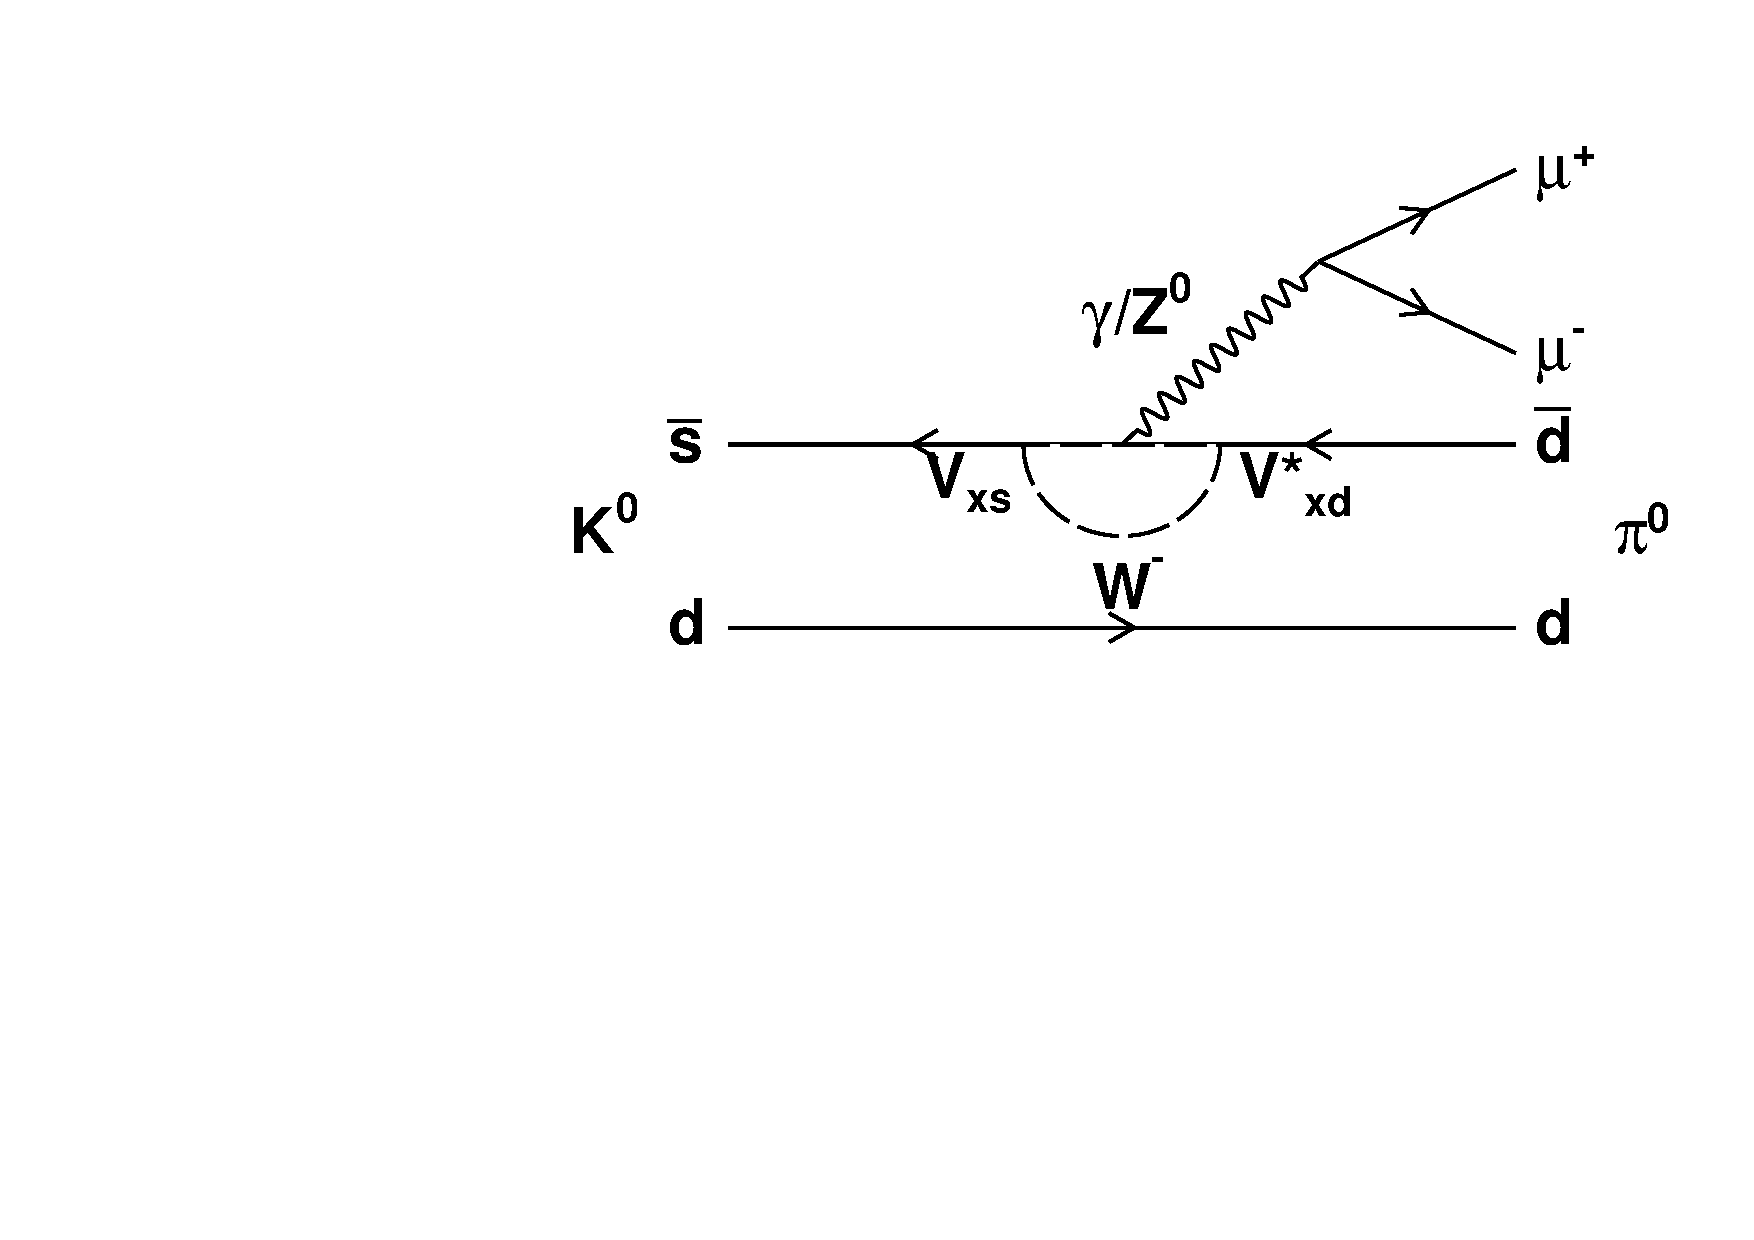
\includegraphics[scale=0.5]{figs/ks_pi0mumu.pdf}
\caption{Feynman diagram of the process \Kzpizmm. \label{fig:diagram}}
\end{center}
\end{figure}

%%% Ks MuMu motivation
\red{Missing connector}\\
Leptonic decays of pseudoscalar mesons with down-type quarks are known to be very sensitive to the Higgs sector of the Minimal Supersymmetric Standard Model (MSSM), due to, among others, enhancement factors proportional to $\left(\tan^6\beta/M_A^4\right)$.\footnote{Note that this enhancement factor is not present in the up-type quark case.} 
This factor comes from the so-called non-holomorphic Yukawa terms at large $\tan \beta$ \cite{Hamzaoui:1998nu,Babu:1999hn,Chankowski:2000ng,Bobeth:2001sq,Isidori:2001fv,Isidori:2002qe},\footnote{
The higher-order contributions have been derived up to two-loop level in refs.~\cite{Crivellin:2010er, Crivellin:2011jt, Crivellin:2012zz}.} which are triggered by the supersymmetric (SUSY) $\mu$ term, and hence the non-SUSY two-Higgs-doublet model cannot produce this enhancement \cite{Isidori:2001fv}. The best known example is $B_s^0\rightarrow\mu^+\mu^-$ \cite{Hamzaoui:1998nu,Babu:1999hn,Chankowski:2000ng,Bobeth:2001sq, Isidori:2001fv,Isidori:2002qe,Choudhury:1998ze,Huang:2000sm,Xiong:2001up,Dedes:2001fv,Bobeth:2002ch,Baek:2002rt,Dedes:2002zx, Mizukoshi:2002gs,Baek:2002wm}. 

If Minimal Flavour Violation (MFV) is imposed, then $B_s^0\rightarrow\mu^+\mu^-$ is the dominant constraint in $P\rightarrow\mu^+\mu^-$ decays. This is due to the stronger Yukawa coupling of the $b$--quark compared to the $s$--quark, and to the better experimental precision in $B_s^0\rightarrow\mu^+\mu^-$ compared to $B_d^0\rightarrow\mu^+\mu^-$. However, in the presence of new sources of flavour violation, the sensitivity of each mode depends on the flavour and $CP$ structures of the corresponding terms.

Hence, a priori, $B_s^0\rightarrow\mu^+\mu^-$, $B_d^0\rightarrow\mu^+\mu^-$, $K_S^0\rightarrow\mu^+\mu^-$, and $K_L^0\rightarrow\mu^+\mu^-$ are all separate constraints that carry complementary information in the general MSSM. The observables related to these decay modes are typically branching fractions and $CP$ asymmetries. Even though the muon polarization could carry interesting information, it cannot be observed by current experiments.


%%% LHCb and kaons
Even though the LHCb experiment \textcolor{red}{ref} was not initially designed to study these particles, the large amount of kaons produced at LHCb \textcolor{red}{ref} makes them a rich area to study. \textcolor{red}{more}It has demonstrated very good performance in the search for rare leptonic \KS decays~\cite{Ksmm}. In the following sections, we evaluate the potential sensitivity of LHCb to \BRof\Kspizmm considering the data to be collected with the LHCb detector before and after its upgrade in 2018, as well as supersymmetric contributions to the decay \KsMuMu in light of current experimental data. 

\begin{comment}
If this New Physics stands at energies higher than the TeV, its effect in quark flavour physics would be visible only with new sources of Flavour Violation not originating from the Yukawa couplings (non Minimal Flavour Violating, non-MFV). In this scenario, the $s \rightarrow d$ decay processes (see Fig. 1) play a central role. This is because they have the strongest CKM suppression factor of all quark transitions ($\prop V_{td}V_{ts} \sim 10^{-4} $), which makes them particularly sensitive to non-MFV sources.
\end{comment}

\section{\Kspizmm Sensitivity study}
\ref{Intro is missing}\\
%% $Id: introduction.tex 87303 2016-02-08 13:44:29Z lafferty $

\section{Introduction}
\label{sec:Introduction}

The $s\to d$ decay processes (see \figref{fig:diagram}) have the strongest CKM suppression factor of all quark transitions.
Hence, they are particularly sensitive to sources of flavour violation different from those of the
Standard Model (SM). Indeed, flavour violation can induce detectable effects at accessible energy in flavour-changing processes
even if the scale of the new dynamics is heavy and well above their direct production at accelerators.
Among these transitions, the decay \Klpizmm has been shown to be sensitive to, for example, models
with extra dimensions~\cite{Bauer:2009cf}. However, the potential for this decay to constrain scenarios
beyond the Standard Model is limited by the large SM uncertainty on its branching fraction prediction~\cite{Bauer:2009cf},%~\cite{D'Ambrosio:1998yj} 
\begin{equation}
{{\cal B}({\PKzL}\to\Pgpz\APmuon\Pmuon)_{\rm SM} = \{1.4\pm0.3; 0.9\pm0.2\}\times 10^{-11}.}
\end{equation}
The two numbers in the brackets correspond to two theoretical solutions, 
depending on whether constructive or destructive interference between the contributing waves is present.
The reason for the large theoretical uncertainty on ${\cal B}({\PKzL}\to\Pgpz\APmuon\Pmuon)_{\rm SM}$ is the limited
precision on the chiral-perturbation-theory parameter $|a_S|$. An improved measurement of \BRof\Kspizmm will reduce this uncertainty.
%\noindent compared to the experimental value:
%\begin{equation}
%{\cal B}({\PKzL}\to\Pgpz\APmuon\Pmuon)_{\rm exp} < 3.8\times 10^{-10}
%\end{equation}
% which is due to the limited experimental precision on \BRof\Kspizmm. 
The most precise measurement of \BRof\Kspizmm was performed by the NA48 experiment at CERN~\cite{NA48}, which obtained
\begin{equation}
{\cal B}({\PKzS}\to\Pgpz\APmuon\Pmuon) = (2.9^{+1.5}_{-1.2}\text{(stat)}\pm0.2\text{(syst)})\times10^{-9}.
\label{eq:NA48}
\end{equation}

\begin{figure} [htb!]
\begin{center}
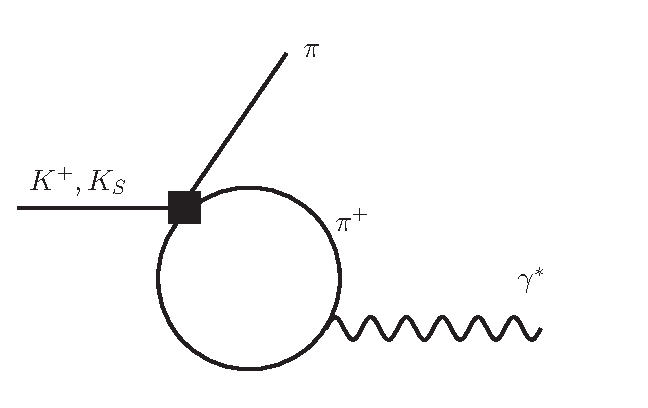
\includegraphics[scale=0.5]{figs/Cirigliano_fig17.pdf} %ks_pi0mumu.pdf}
\caption{Feynman diagram of the process \Kzpizmm. \label{fig:diagram}}
\end{center}
\end{figure}

The LHCb experiment~\cite{LHCbDet} has demonstrated very good performance in the search for rare leptonic \KS decays~\cite{Ksmm}. In this note, we evaluate the potential
sensitivity of LHCb to \BRof\Kspizmm considering the data to be collected with the LHCb detector before and after its upgrade in 2018.
 
This document is organized as follows: in~\secref{sec:strategy}, the analysis strategy is summarized; in \secref{sec:selection}, details on the signal reconstruction and selection are given;
in \secref{sec:background}, the study on the expected background sources is presented; in \secref{sec:fit}, the likelihood fit is described; in~\secref{sec:sensitivity}, the sensitivity to
\BRof\Kspizmm is reported and finally, conclusions are drawn in~\secref{sec:conclusions}.

% $Id: introduction.tex 87303 2016-02-08 13:44:29Z lafferty $

\subsection{Analysis strategy}
\label{subsec:strategy}

Decays of the \KS in LHCb are characterized by decay vertices separated from the interaction point\footnote{The \KS at LHC typically decays after traversing tens of centimeters to even several meters.}, 
and with tracks having an average transverse momentum significantly lower than those from $b$ and $c$ decays.
The transverse momentum range is similar to typical tracks generated in the proton-proton collision and hence has almost no discriminating power. 

Muon candidates are combined into $\mu^+\mu^-$ pairs. Then a $\pi^0$ can be added to the dimuon pair to make a fully reconstructed
\KS decay. However, since the reconstruction efficiency of the $\pi^0$ is limited, events in which no $\pi^0$
is found are also considered, based only on the dimuon information. This leads to two independent analyses: one for the
events in which all decay products are considered (hereafter FULL) and one in which only the dimuon pair is used
(hereafter PARTIAL). 
The reconstructed candidates are then passed through a selection algorithm followed by a {\it Boosted Decision Tree} (BDT) classification,
to reduce the high level of background.


The properties of the \Kspizmm decays are studied using simulated samples with a differential decay rate modeled according to Ref.~\cite{Gino}.
The corresponding $\mumu$ mass distribution, $m_{\mumu}$, as well as the dependence of the (cosine of the) dimuon helicity 
angle, $\cos\theta_{\mu}$ (see the angle definitions in \figref{fig:angles}), on $m_{\mumu}$ are shown in \figref{fig:EviltGen}.

 \begin{figure}[htb!]
 \begin{center}
  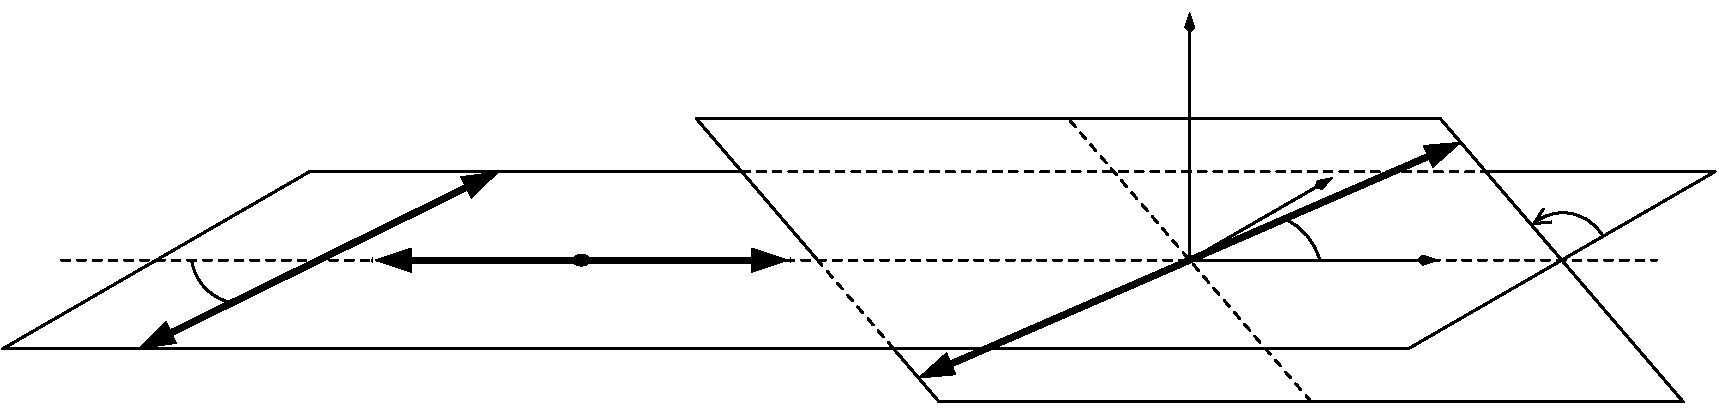
\includegraphics[scale=0.4]{figs/Kspi0MuMu/helAngles.pdf}
  \put(-27,40){${\phi_{\mu}}$}
  \put(-70,35){${\theta_{\mu}}$}
  \put(-308,21){${\phi_{\pi}}$}
  \put(-64,54){$\mu^{-}$}
  \put(-142,5){$\mu^{+}$}
  \put(-272,34){$\pi^0$}
  \put(-225,36){$\KS$}
  \put(-275,18){$\gamma$}
  \put(-250,34){$\gamma$}
  \caption{Definition of the helicity angles in the \KS\ rest frame. \label{fig:angles}}
  \end{center}

 \end{figure}

\begin{figure} [htb!]
\begin{center}
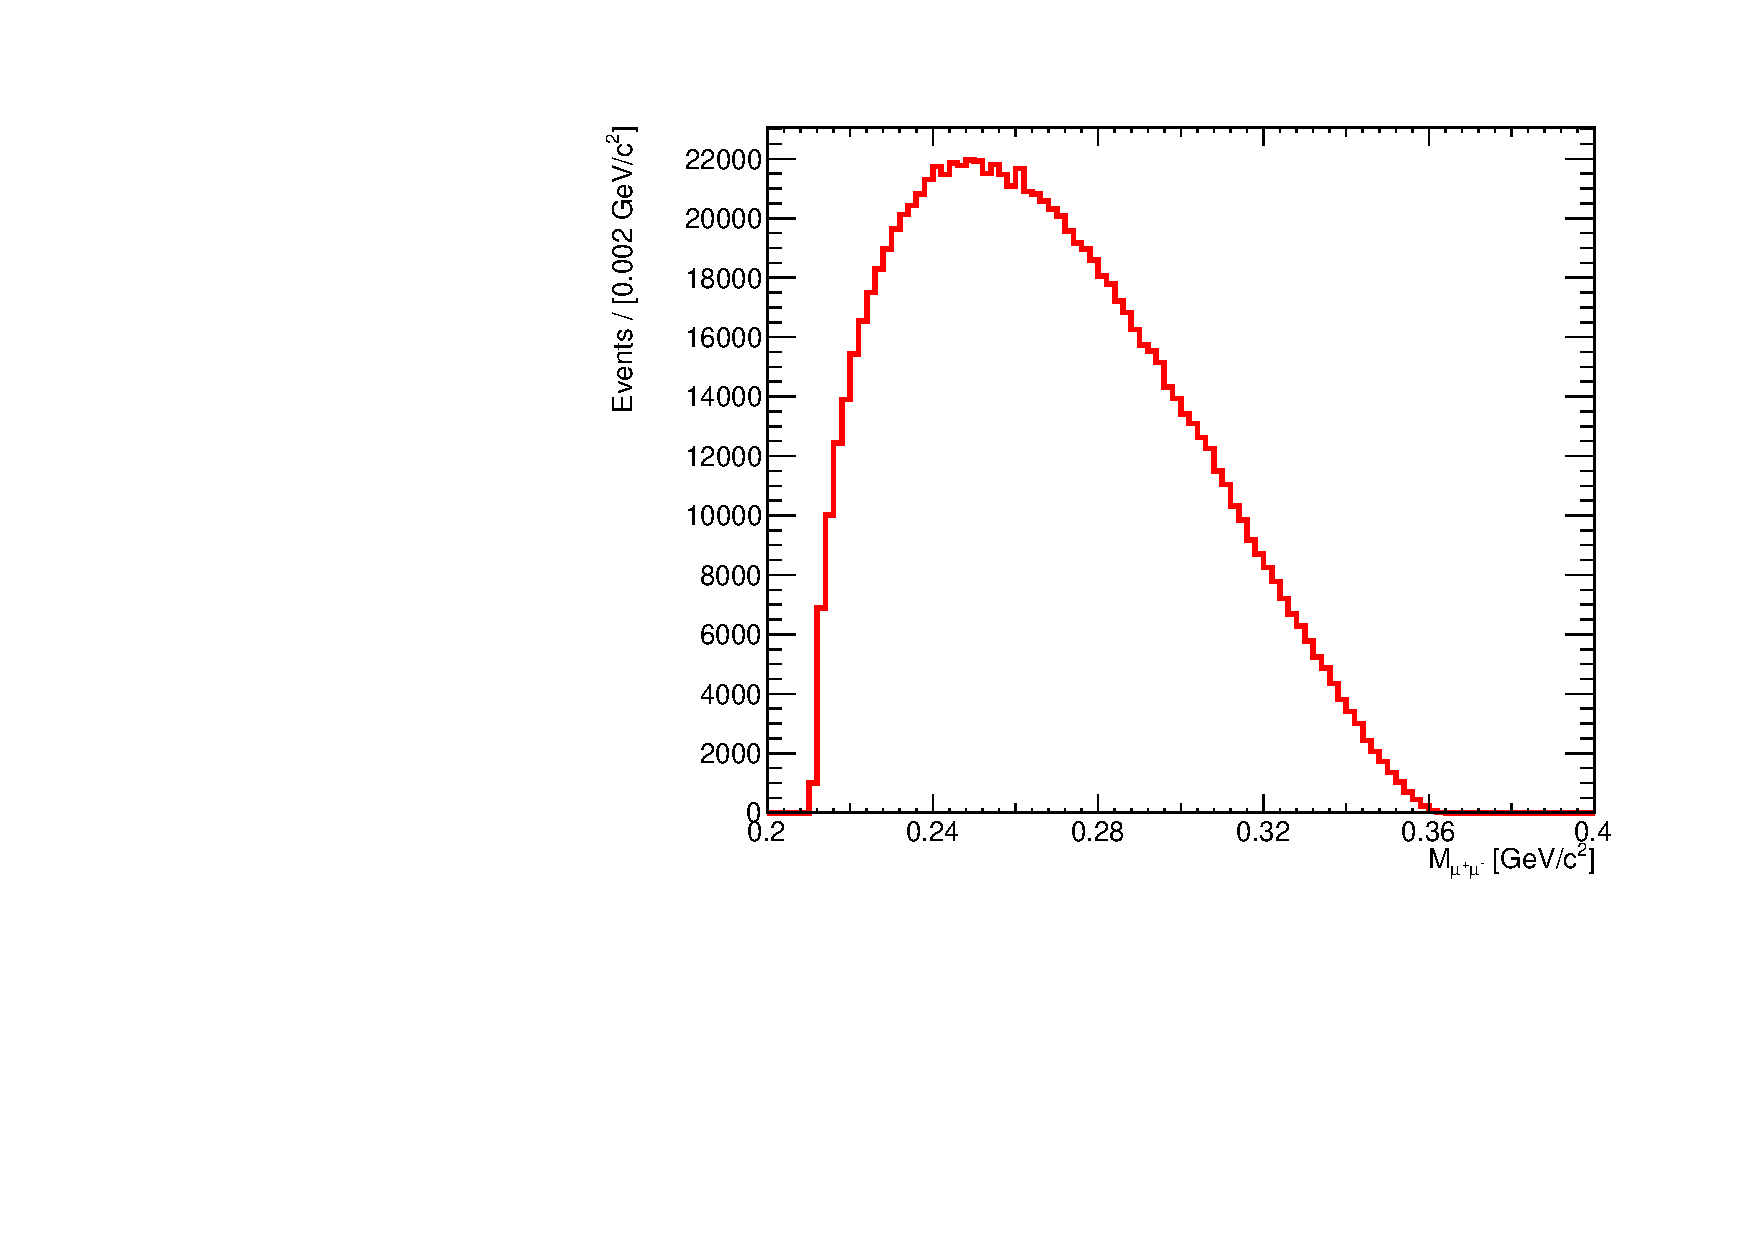
\includegraphics[scale=0.35]{figs/Kspi0MuMu/M_mumu.pdf}
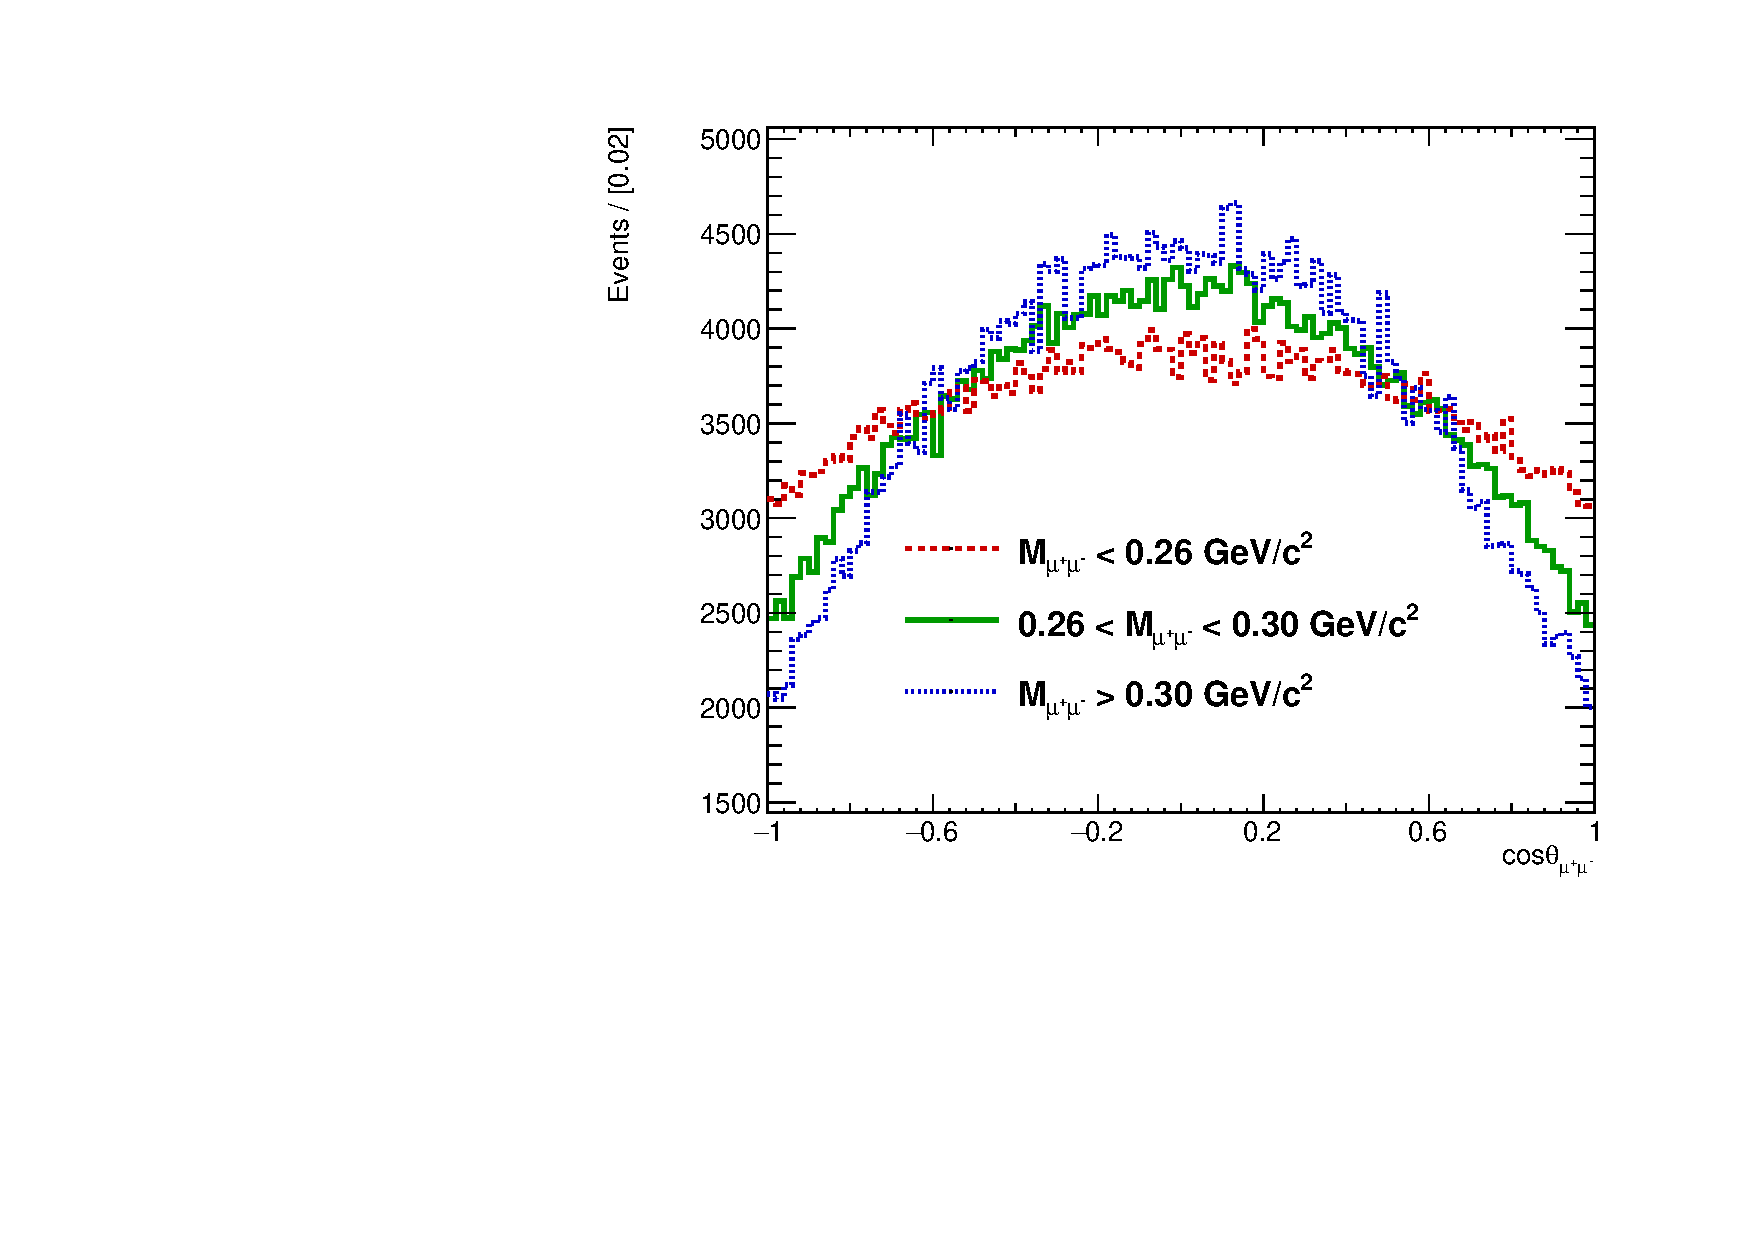
\includegraphics[scale=0.35]{figs/Kspi0MuMu/Hel_mumu.pdf}
\caption{$m_{\mu\mu}$ distribution (left), and the dimuon helicity angle depending on $m_{\mu\mu}$ (right). \label{fig:EviltGen}}
\end{center}
\end{figure}


The BDT is trained with simulated signal events and combinatorial background events from the existing LHCb data.
Since the main goal of this study is to evaluate the sensitivity for the LHCb upgrade, where the
trigger efficiency is expected to be very high, trigger unbiased data samples are preferred.
Therefore, the events are obtained from the {\it Trigger Independent of Signal} (TIS) ~\cite{TISTOS} category of the LHCb trigger. 
This means that the tracks and clusters of the reconstructed candidate are not needed to fire the trigger at any level, because
another object in the underlying event already fired it.
This ensures an almost trigger unbiased data set, while still providing a sample much larger than random selection triggers. 

%The expected signal yield is obtained assuming the NA48 central value for \BRof\Kspizmm, the observed \Kspipi yield from data and
%the efficiency ratio \textcolor{red}{$\frac{\epsilon_{\KsPzMuMu}}{\epsilon_{\PKzS\to\Pgpp\Pgpm}}$} obtained in simulation (See \eqref{eq:normalization}). 

The expected signal yield is obtained assuming the NA48 central value for \BRof\Kspizmm, normalizing the signal yield with respect to \Kspipi as 
\begin{equation}
      \frac{N(\KsPzMuMu)}{N(\PKzS\to\Pgpp\Pgpm)} = 
      \frac{{\cal B}(\KsPzMuMu){\epsilon_{\KsPzMuMu}}}
      {{\cal B}(\PKzS\to\Pgpp\Pgpm){\epsilon_{\PKzS\to\Pgpp\Pgpm}}},
\label{eq:normalization}
\end{equation}
where the observed \Kspipi yield is extracted from data and the efficiency ratio, $\frac{\epsilon_{\KsPzMuMu}}{\epsilon_{\PKzS\to\Pgpp\Pgpm}}$, is obtained from simulation.

The \BRof\Kspizmm sensitivity is measured in a pseudo-experiment study. First, the signal and background yields are extrapolated
for a desired expected luminosity and trigger efficiency, then pseudo-experiments are generated according to those yields. 
The \BRof\Kspizmm uncertainty is obtained from a fit to the \KS mass distribution of the pseudo-experiments, using the signal and background
models obtained from MC and the fit to the available LHCb data, respectively. The mass fit range is $[420,580] \mevcc$.
 



% $Id: introduction.tex 87303 2016-02-08 13:44:29Z lafferty $

\subsection{Reconstruction and selection}
\label{subsec:selection}

Pairs of muon candidates are reconstructed combining opposite-charged tracks with hits in the vertex locator (VELO), trigger tracker, tracker stations, and muon chambers. 
In addition, the tracks are required to be separated by at least $6\sigma$ from any $p-p$ collision point in the event.
Tracks with transverse momentum lower than 80\mevc are ignored. 
A dimuon candidate pair can be combined with a $\pi^0$ candidate to build a \KS\ candidate. 
The events in which the entire decay chain is used are classified as FULL. When only the dimuon information is used, they are clasified as PARTIAL.

Neutral pion candidates are reconstructed from 
$\gamma$ candidate pairs that correspond to two independent clusters in the calorimeter.
Each photon candidate is required to have a transverse momentum of
at least 200\mevc and the pion candidate a mass within 30\mevcc of the world average $\pi^0$ mass.
The mass resolution is then improved by constraining the $\pi^0$ candidate 
mass to the world average $\pi^0$ mass, and by constraining the three-momentum
vector of the \KS to point back to the production vertex. For the PARTIAL candidates, a momentum vector with an absolute value of $\approx 10\gevc$
is used as a representative of the $\pi^0$ momentum when calculating the invariant mass. As a consequence of these kinematic constraints, the \KS\ candidate 
mass resolution depends only weakly on the $\pi^{0}$ momentum.

Additional selection requirements are applied to reduce the
amount of data to analyze, fulfil the rate requirements for LHCb offline
processing and reduce the amount of background. These include a \KS\ candidate lifetime of at least $1\;\rm ps$
and removing events in the kinematic region of $\Lambda\to p \pi$ and $\KS\to \pi^{+}\pi^{-}$ in the Armenteros-Podolanski plane~\cite{Armenteros}.
The total reconstruction and selection efficiency for the FULL channel is $5.47\times10^{-4}$.

Requiring a well-reconstructed  $\pi^0$ implies an inefficiency penalty of a factor ten.
Thus, a complementary strategy for the PARTIAL candidates is also investigated.
Indeed, the constraints on the $\pi^0$ mass and the \KS momentum are sufficient to create a peaking distribution if there is an estimate of the typical
value of the $\pi^0$ momentum ($\approx 10\gevc$), as shown in \figref{fig:peaks}.
A comparison of the reconstructed mass resolution between FULL and PARTIAL is difficult due to the asymmetric and non-Gaussian distribution of the PARTIAL case. To get an estimate, the corresponding 
FWHM values are calculated. In the FULL case, it is 23.3~\mevcc and in the PARTIAL 40.6~\mevcc.

The PARTIAL selection does not require any information about a reconstructed $\pi^0$. Some
requirements had to be tightened in order to keep the background at a manageable level. These include a lower distance of closest approach between the two
muon tracks; a minimum requirement on the \KS\ vertex quality, $\chi^{2}/ndof = 9$; a higher minimum requirement on the \KS\ vertex detachment from the interaction point;
and minimum radial, $z$- and absolute distance requirements between the \KS\ vertex and the interaction point.
The total reconstruction and selection efficiency for the PARTIAL analysis is $3.0\times 10^{-3}$ , well above that of the FULL,
but at a cost of an increased background yield.

\begin{figure} [htb!]
\begin{center}
%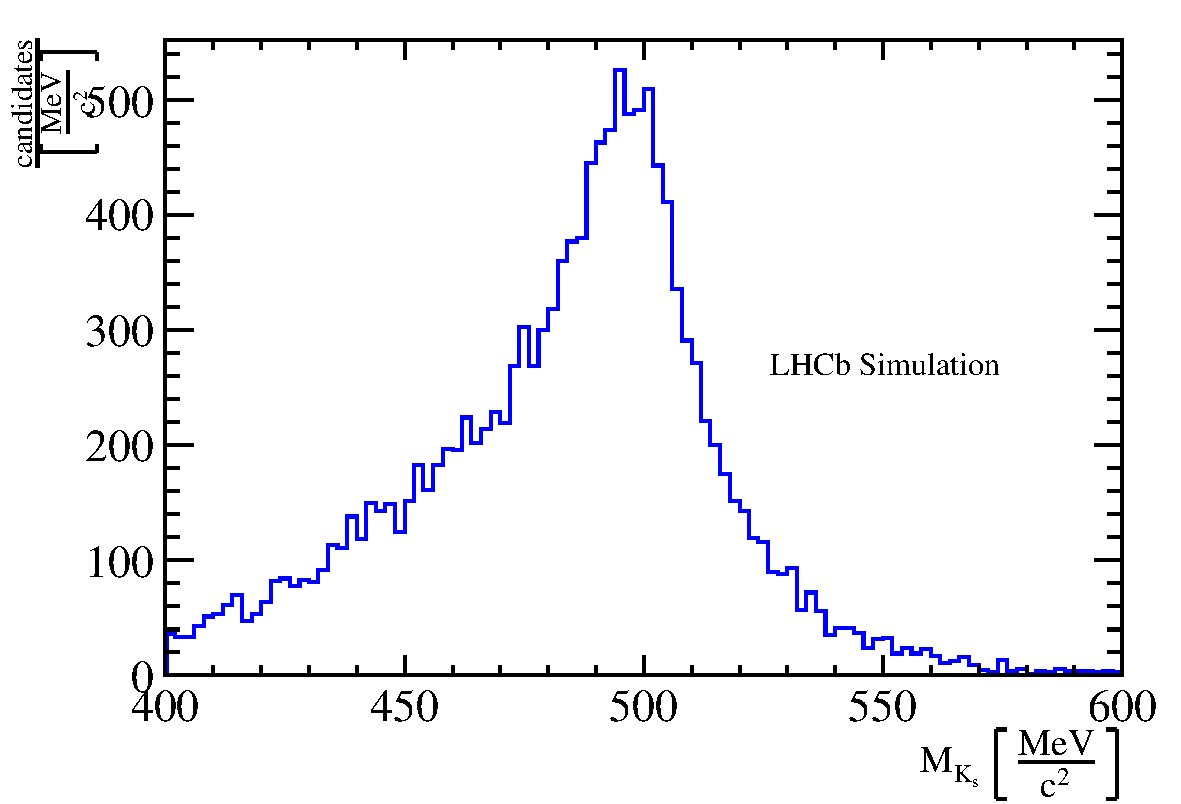
\includegraphics[scale=0.35]{figs/hphantom.pdf}
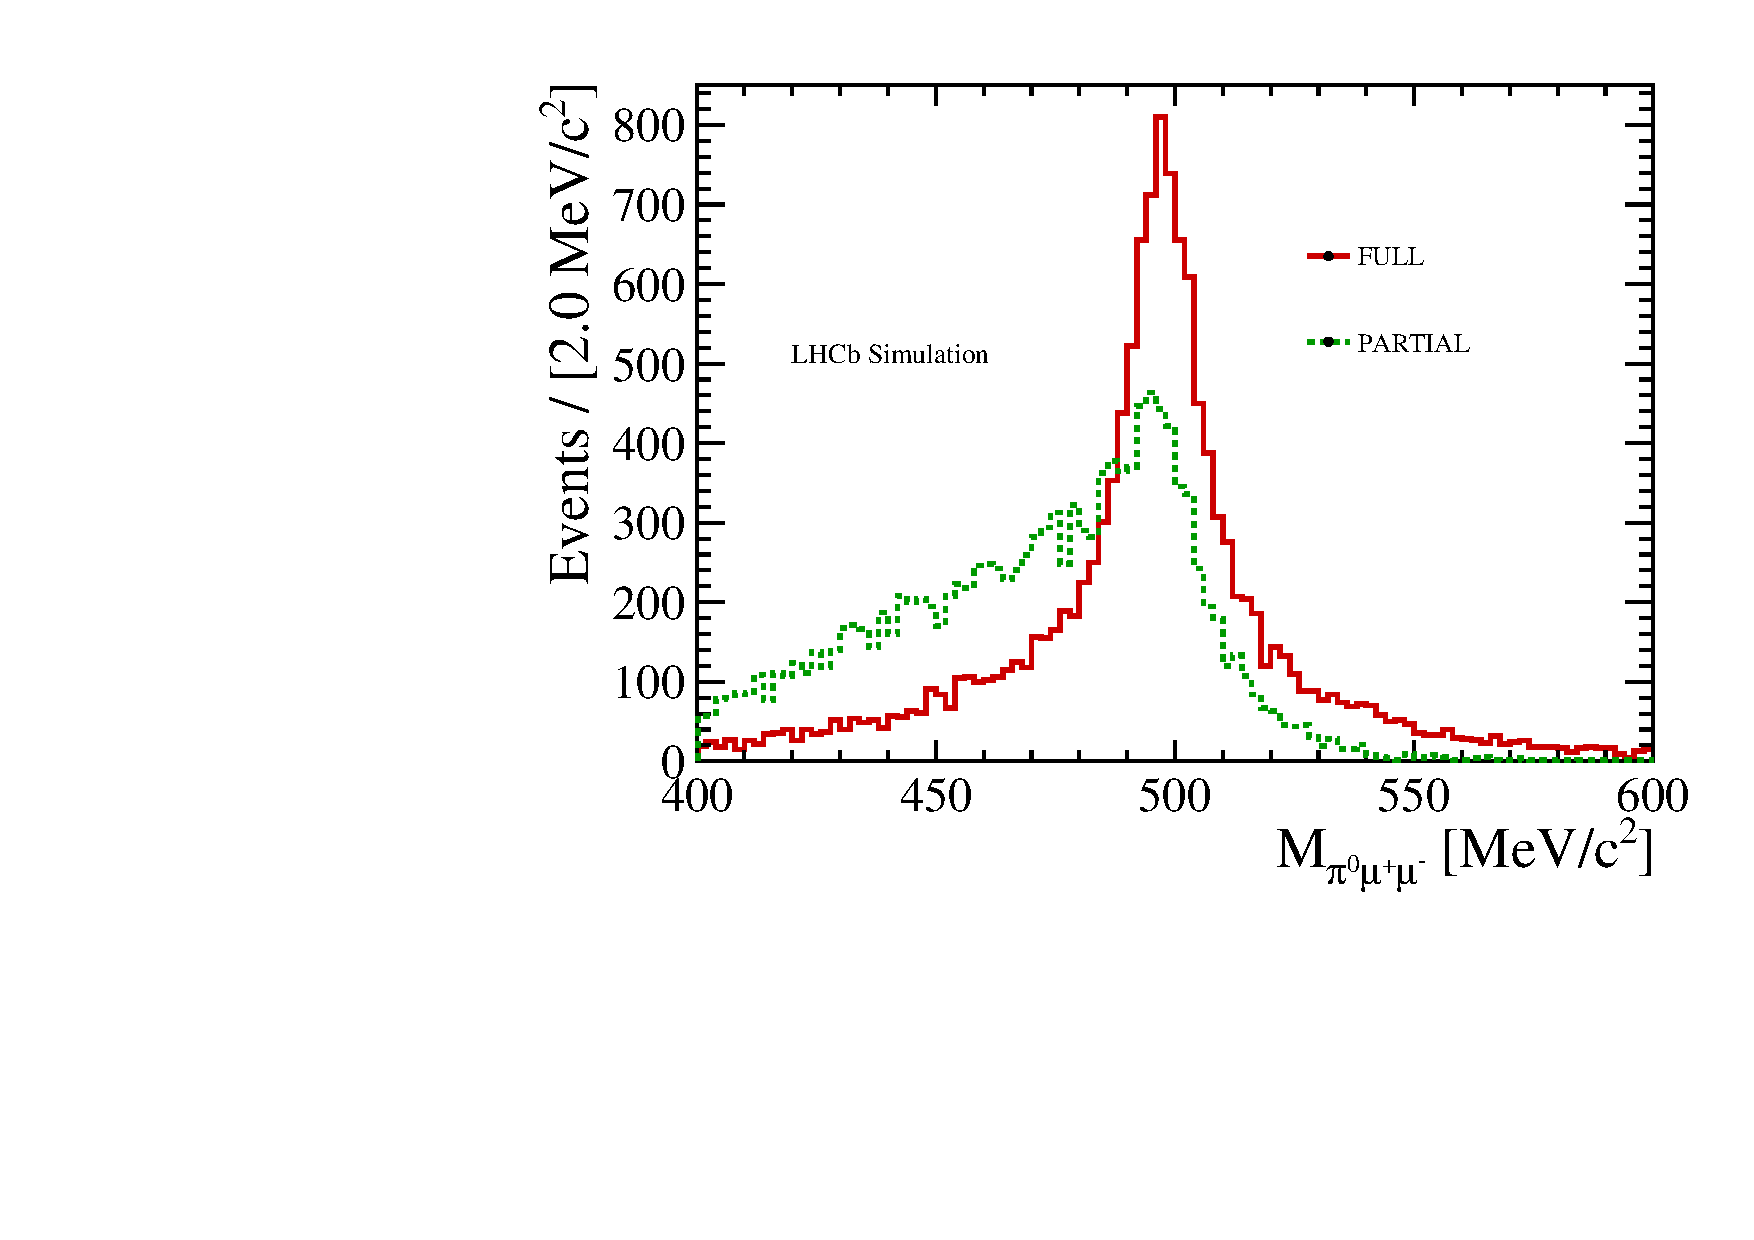
\includegraphics[scale=0.6]{figs/Kspi0MuMu/M_V0_vs_VC.pdf}
\caption{Comparison between the FULL (solid red) and PARTIAL (dashed green) kaon candidate mass distributions. \label{fig:peaks}}
\end{center}
\end{figure}

A BDT is used to separate signal from combinatorial background. It is trained with MC events (signal class) and a part of the data that is not used in the fit
(combinatorial background class). The BDT uses information about the geometrical properties of the events,
kinematics, track quality, and muon identification quality. The BDT response for signal and background for both FULL and PARTIAL 
is shown in \figref{fig:BDT}.


\begin{figure} [htb!]
\begin{center}
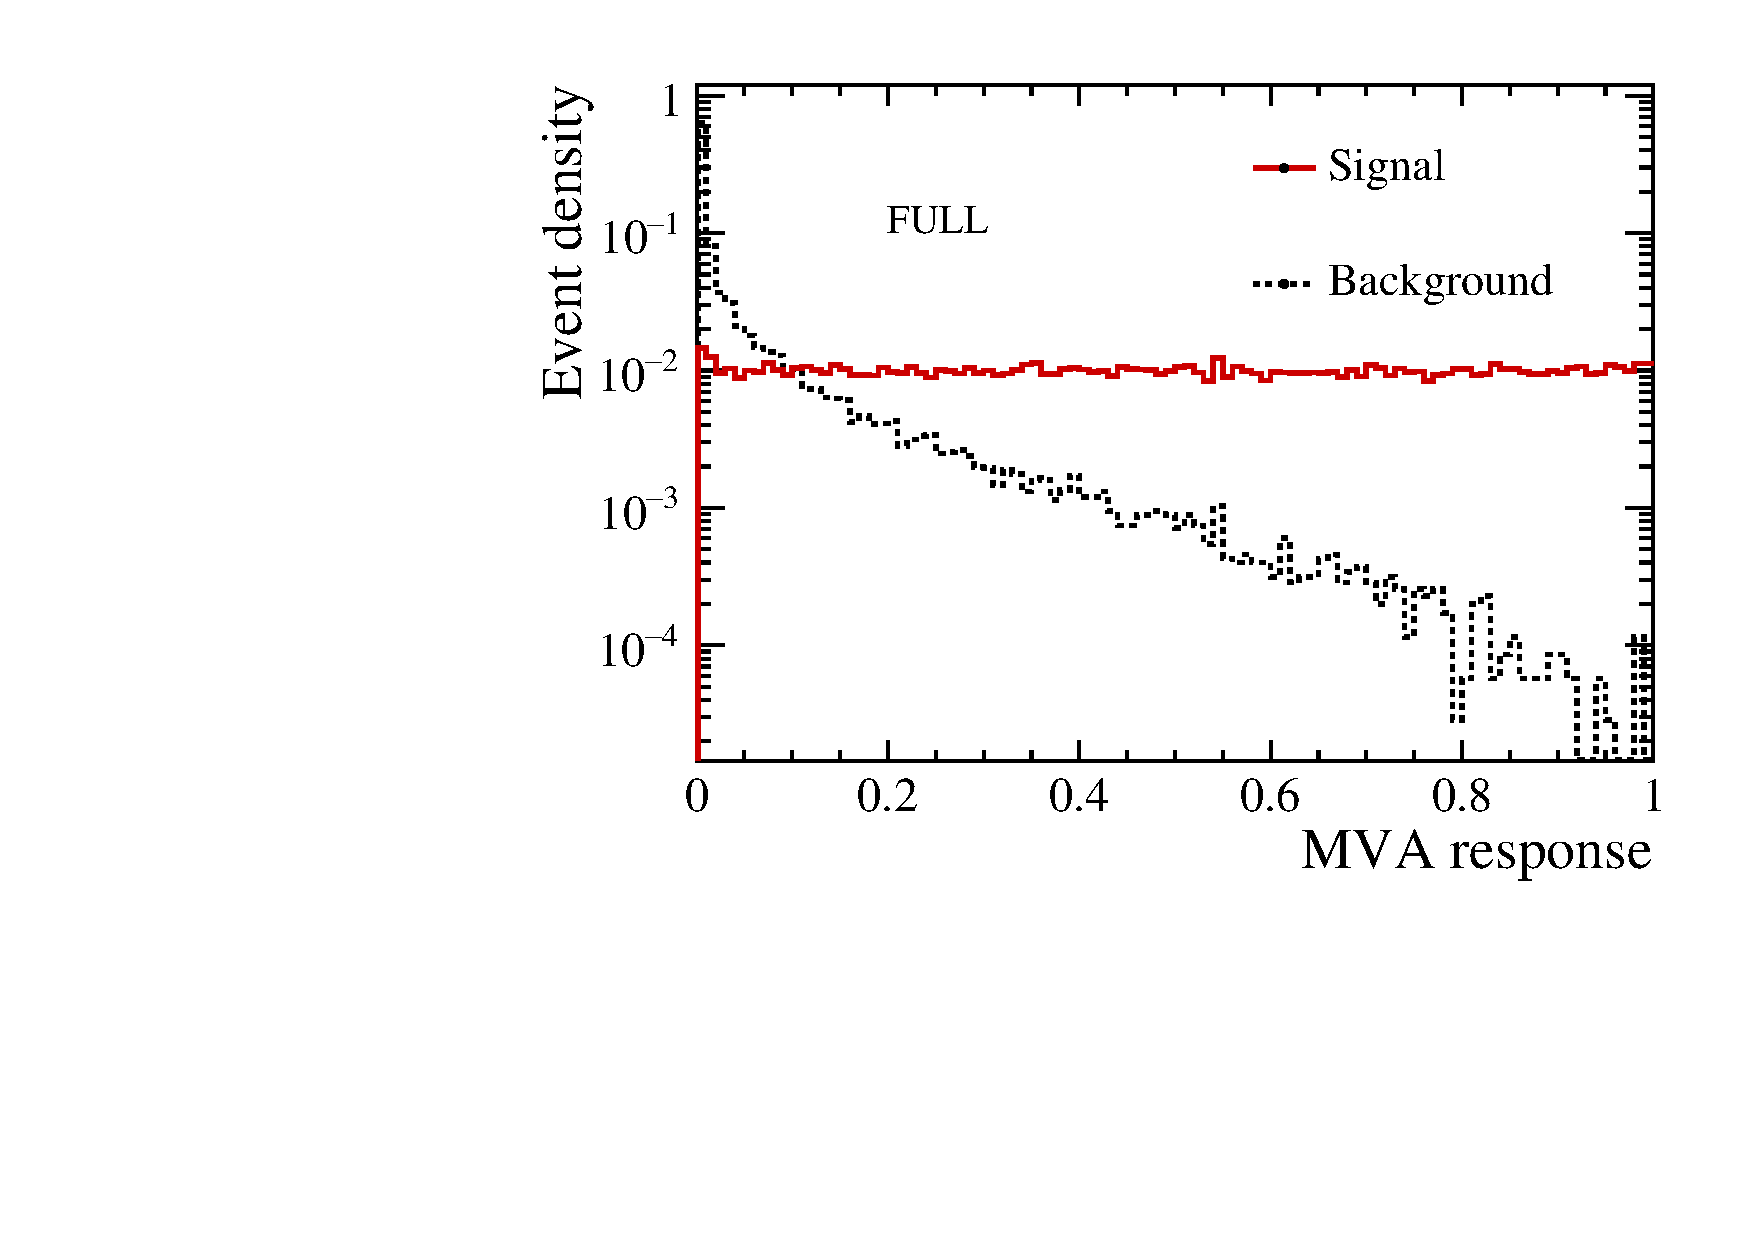
\includegraphics[scale=0.38]{figs/Kspi0MuMu/BDT_sig_vs_bkg_FULL.pdf}%BDTFULL.pdf}
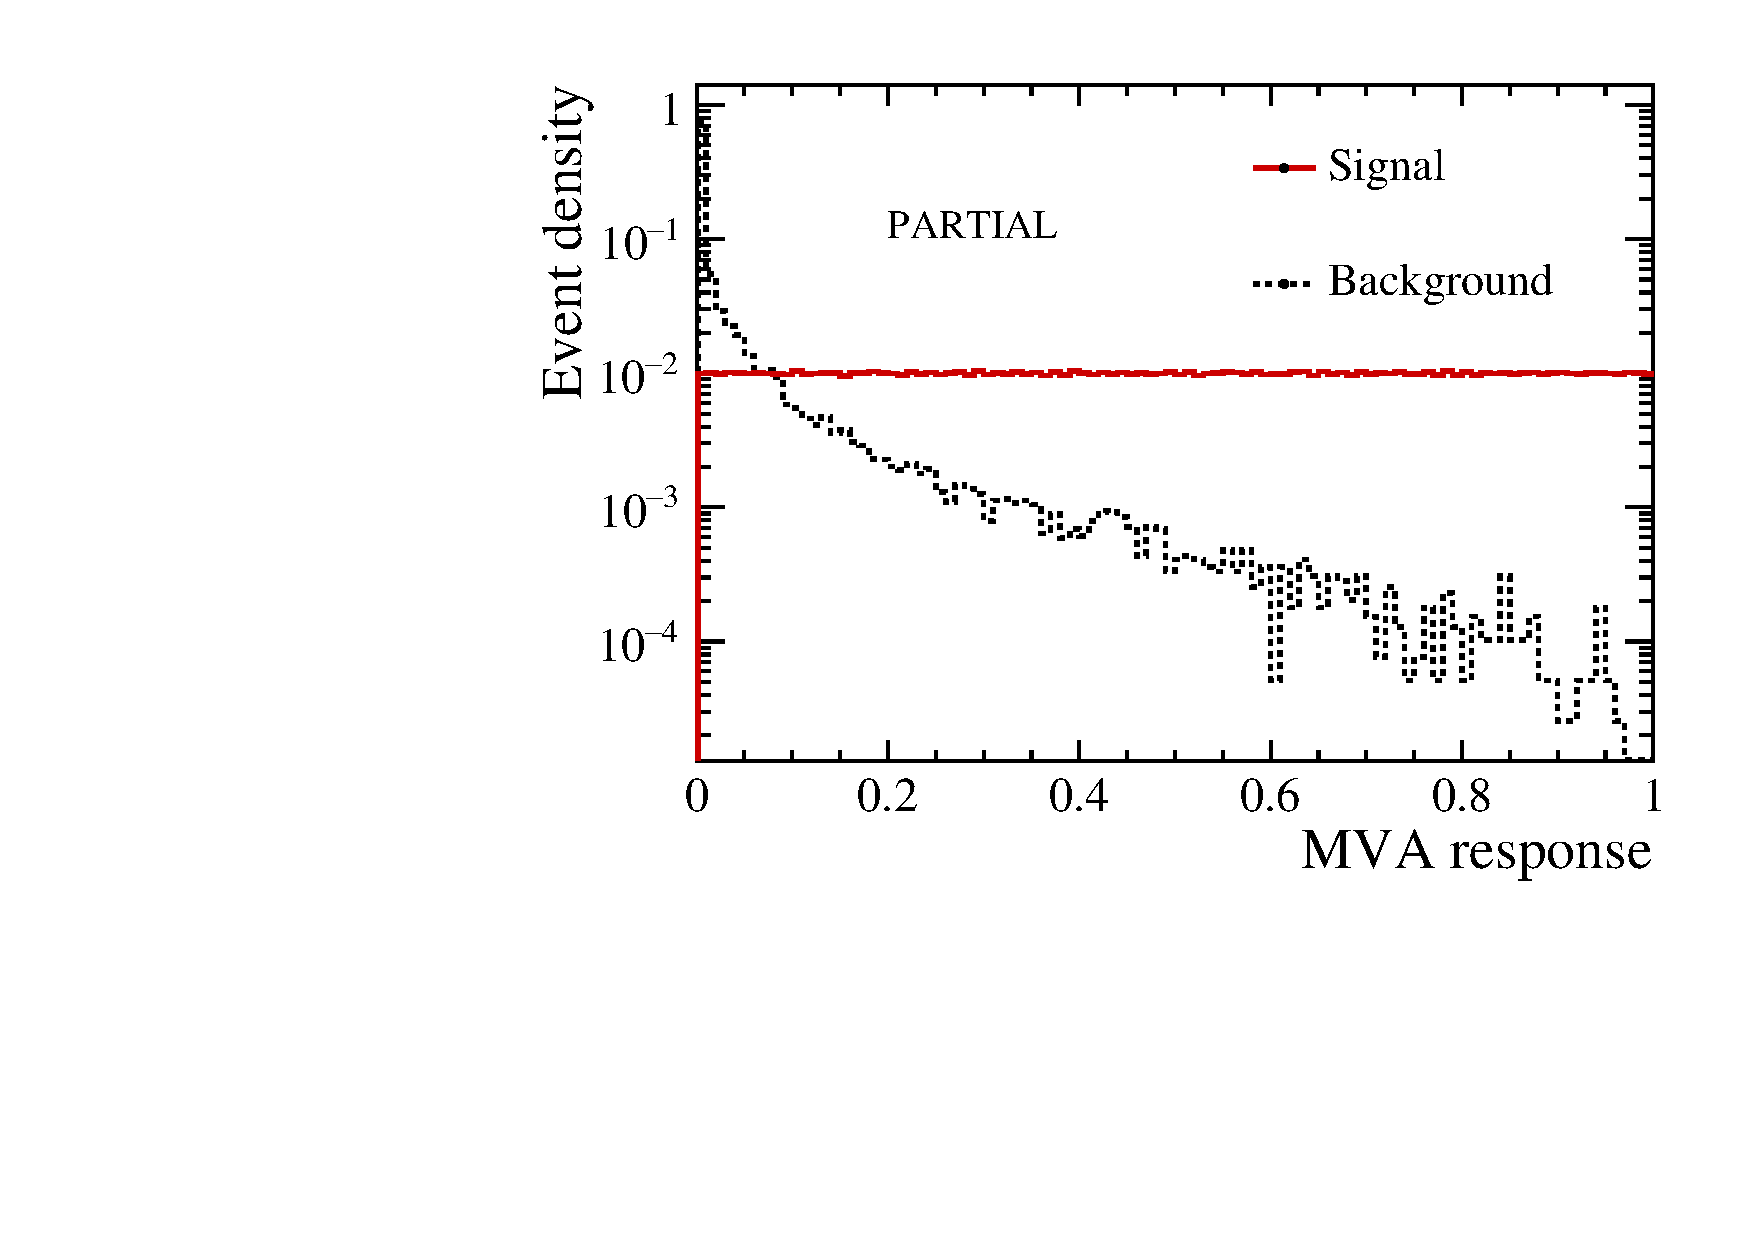
\includegraphics[scale=0.38]{figs/Kspi0MuMu/BDT_sig_vs_bkg_PARTIAL.pdf}%BDTPARTIAL.pdf}
\caption{BDT response both for signal (solid red) and background (dashed black). Right: FULL channel. Left: PARTIAL channel.  Signal and background are normalized to the same area. \label{fig:BDT}}
\end{center}
\end{figure}


The events are classified in four bins of the BDT response. The signal yields are obtained in a simultaneous fit 
of the mass distribution in each BDT bin, as described in the following sections.

% $Id: introduction.tex 87303 2016-02-08 13:44:29Z lafferty $

\subsection{Background sources}
\label{subsec:background}

Several sources of background are investigated to assess their relevance for a measurement of \BRof\Kspizmm:
\begin{itemize}
%\item Misidentified \Kspipi decays (combined with a combinatorial $\pi^0$ in the case of FULL). 
\item \Kspipi decays, where both pions are misidentified as muons, and in the case of the FULL category, combined with a random $\pi^0$ from the underlying event.
These decays have a mass larger than that of the \KS and do not enter the fit region, except for potential residual tails that effectively add up to the combinatorial background. % TODO (see \figref{fig:Kspipibkg}). 
No evidence for \Kspipi background is seen for the BDT region being fitted. 
\item \KTmTg decays. This background was considered in the NA48 analysis ~\cite{NA48}, 
However, its contribution at LHCb is found to be negligible: In the case of the \KL decay (with a branching fraction of $1.0^{+0.8}_{-0.6}\times10^{-8}$ ~\cite{PDG}) the upper decay time acceptance introduces 
an effective $10^{-3}$ reduction with respect to \KS and hence
the effective \BRof\KLTmTg becomes as low as $10^{-11}$. There is no experimental measurement of \BRof\KSTmTg, however, since
the process is dominated by the two-photon exchange\footnote{Isidori and D'Ambrosio, private communication.}, it can be estimated as:
\begin{equation}
\BRof\KSTmTg = \frac{\BRof\KSTg}{\BRof\KLTg}\BRof\KLTmTg \sim 4.8\times10^{-11}
\end{equation} 
\noindent and is thus negligible.
\item \KLTpi decays. The mass distribution of these decays is shown in \figref{fig:KLTpi} as obtained in simulation. Since there is no evidence of this background in the 
data, it is neglected. Including a \KLTpi component to the observed background does not change significantly the sensitivity estimates. The \KS counterpart has a branching fraction of $3.5\times10^{-7}$ and thus
is about four orders of magnitude smaller than \KLTpi. In general, no sign of a resonant structure in the $\pi^+\pi^-\pi^0$ is seen on data.

\item Combinatorial background. Combinatorial background is considered to be composed by random combination of tracks, including those generated by pseudo-random combinations of hits during the pattern recognition. 
It has a monotonic shape across the studied invariant mass range.

\end{itemize}

\begin{figure} [htb!]
\begin{center}
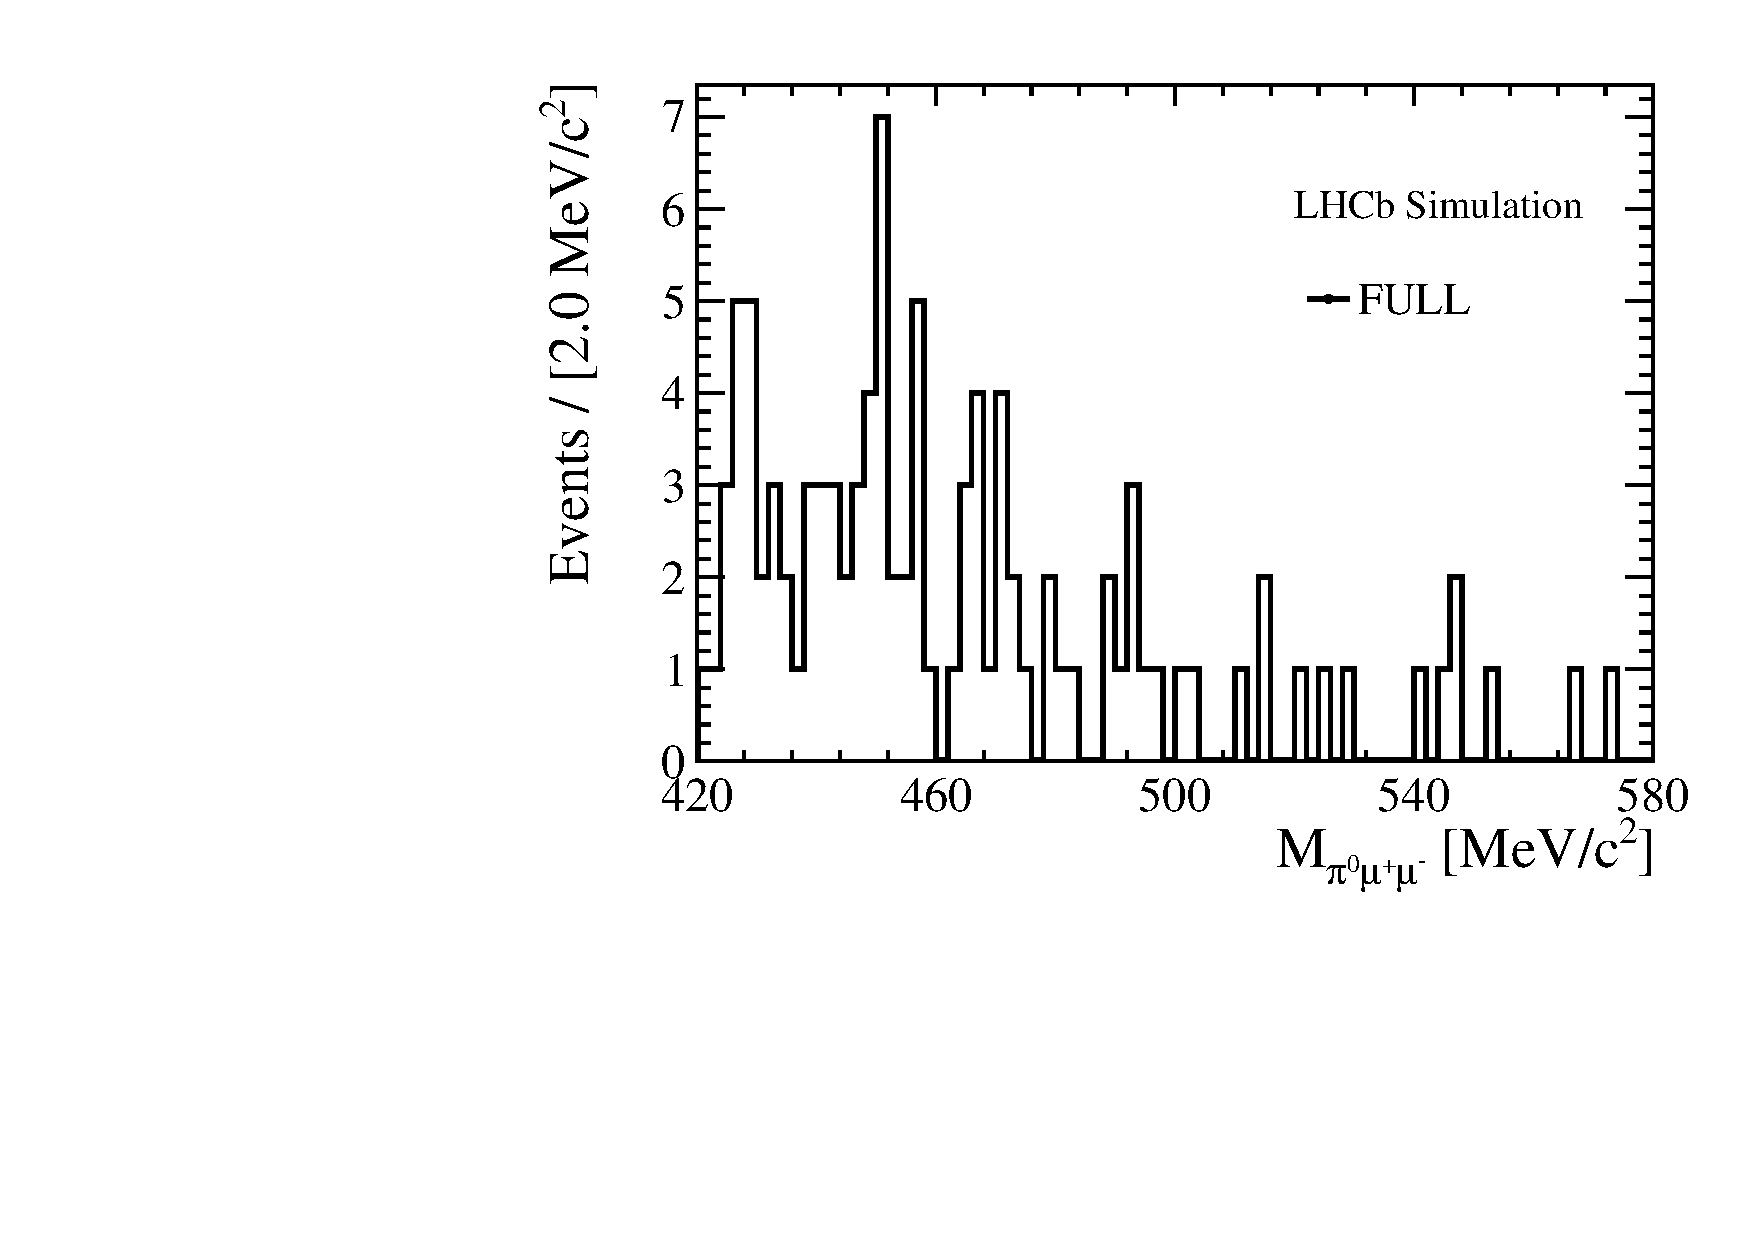
\includegraphics[scale=0.30]{figs/Kspi0MuMu/M_VC_K3pi.pdf}%{figs/K3pi_FULL.pdf}
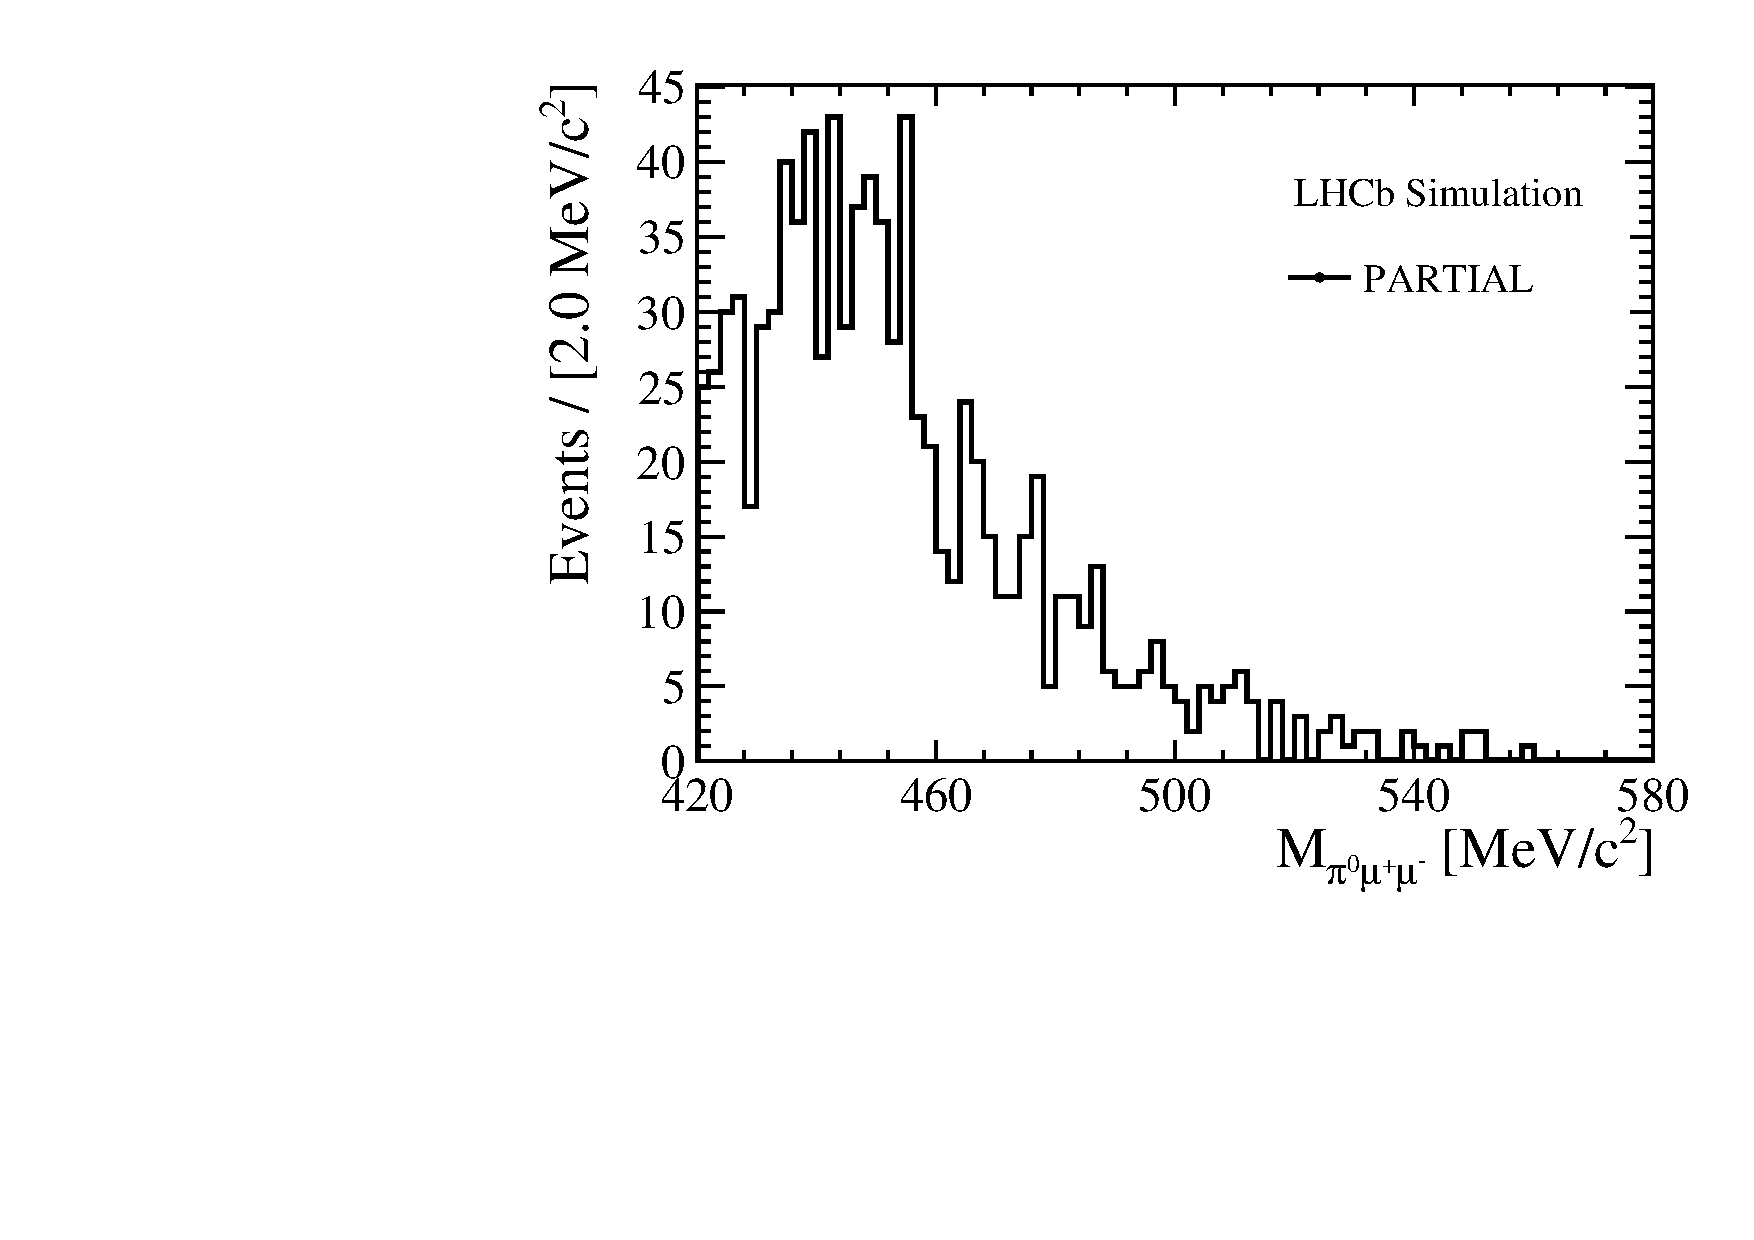
\includegraphics[scale=0.30]{figs/Kspi0MuMu/M_V0_K3pi.pdf}%{figs/mK3pi_PARTIALL.pdf}
\caption{Invariant mass distribution of simulated $K^0\rightarrow\pi^+\pi^-\pi^0$ decays selected in the FULL (left) and PARTIAL (right) categories.  \label{fig:KLTpi}}
\end{center}
\end{figure}


% $Id: introduction.tex 87303 2016-02-08 13:44:29Z lafferty $

\subsection{Fit model}
\label{subsec:fit}
Only events in the BDT range [0.6,1] are considered in the fit to the data.
A simultaneous fit to the mass distribution across four equally-sized
independent bins of the BDT response is performed. The combinatorial background is described
with an exponential \pdf for both FULL and PARTIAL analysis, with independent floating yields and
decay constants in each BDT bin. The signal
model is an Hypathia distribution~\cite{Ipatia} with different configurations
for FULL and PARTIAL (see \figref{fig:Ipatia}). The signal model parameters are independent
in each BDT bin and are obtained from simulation. The fractions of signal events allotted to each
BDT bin are also fixed from values obtained from simulation, with a total signal yield remaining as the sole free parameter describing signal in the simultaneous fit. %%%\textcolor{red}{J: What do you do with the background?}
The signal yield is floated in the fit to the data. It is measured to be 
compatible with zero within one to two sigma. %, given the limited size of the data sample.
The fit projections to the FULL and PARTIAL data are shown in \figref{fig:fit}.% and \figref{fig:fitPARTIAL},respectively.
\begin{figure} [htb!]
\begin{center}
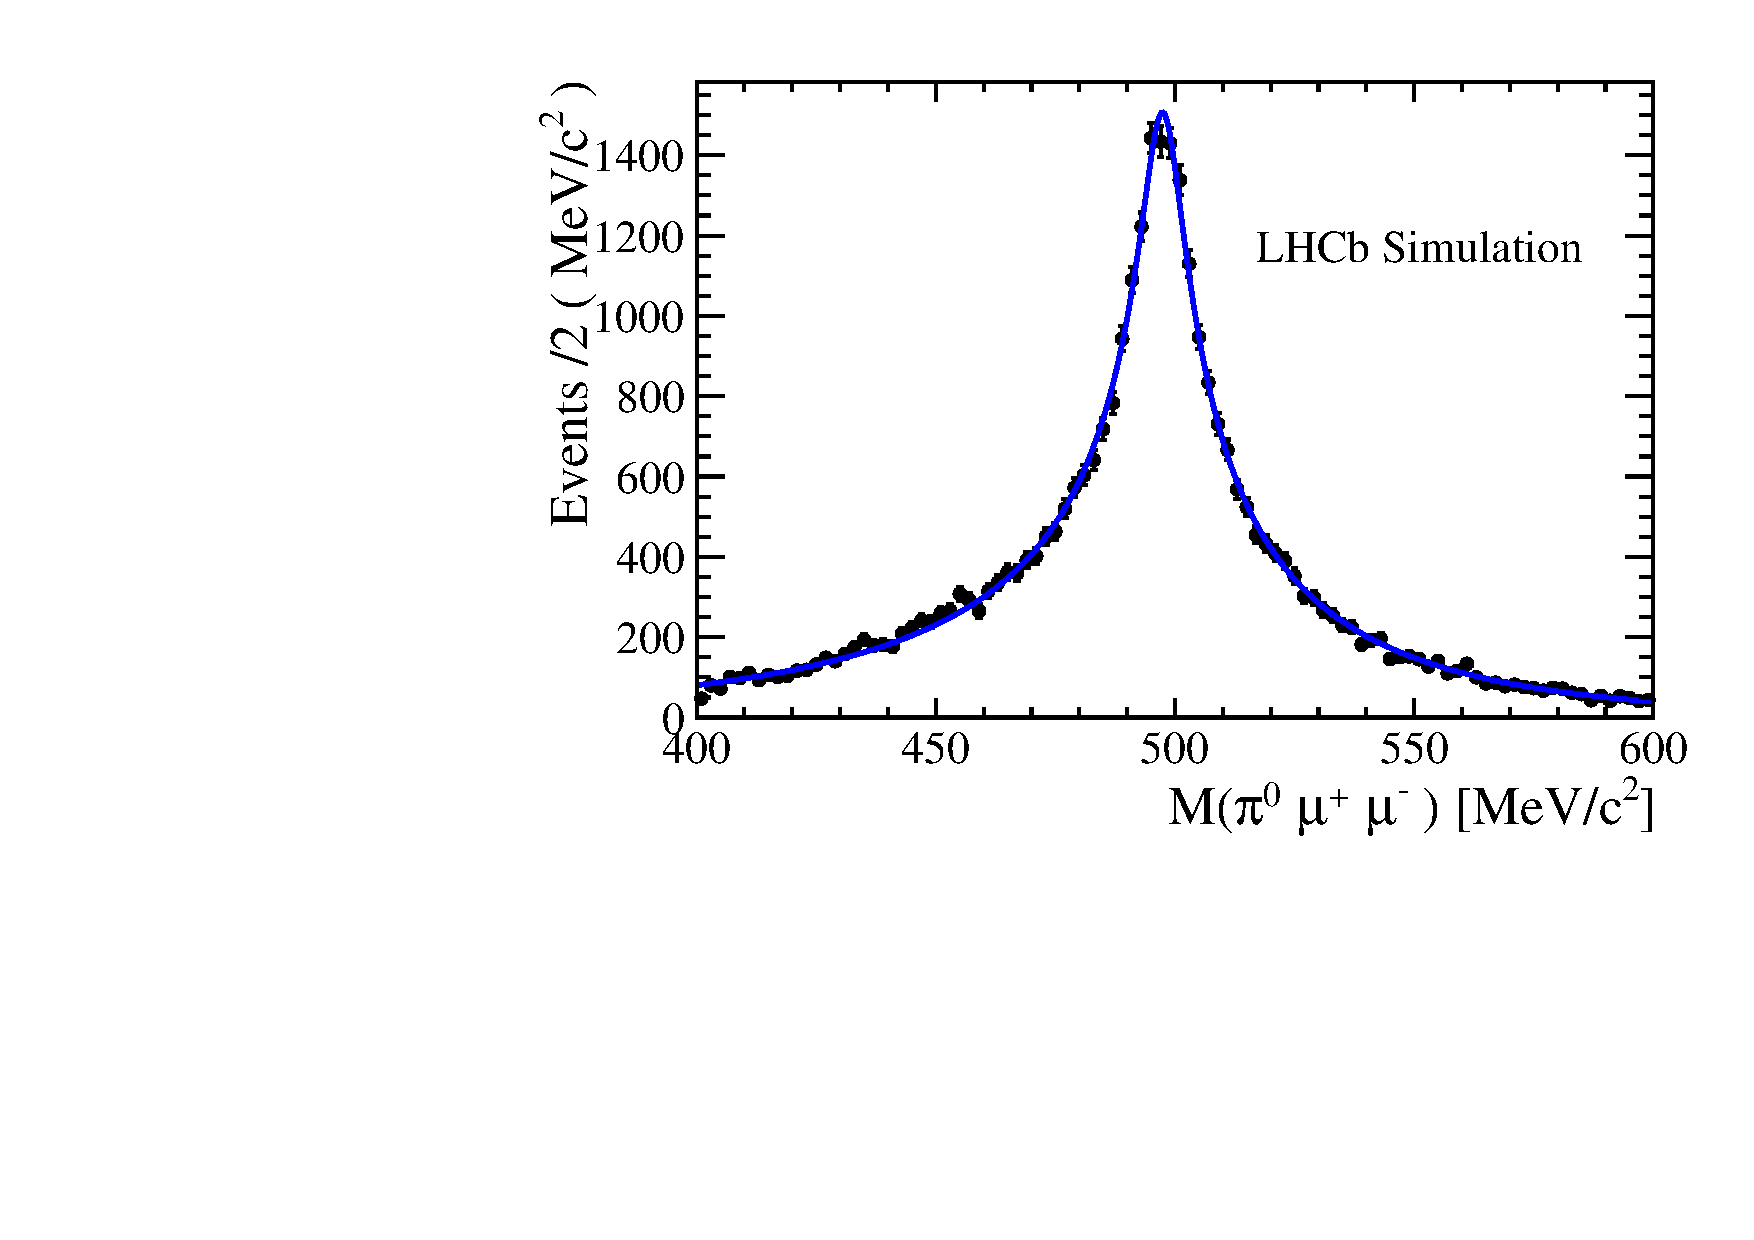
\includegraphics[scale=0.30]{figs/Kspi0MuMu/Ipatia_pi0.pdf}
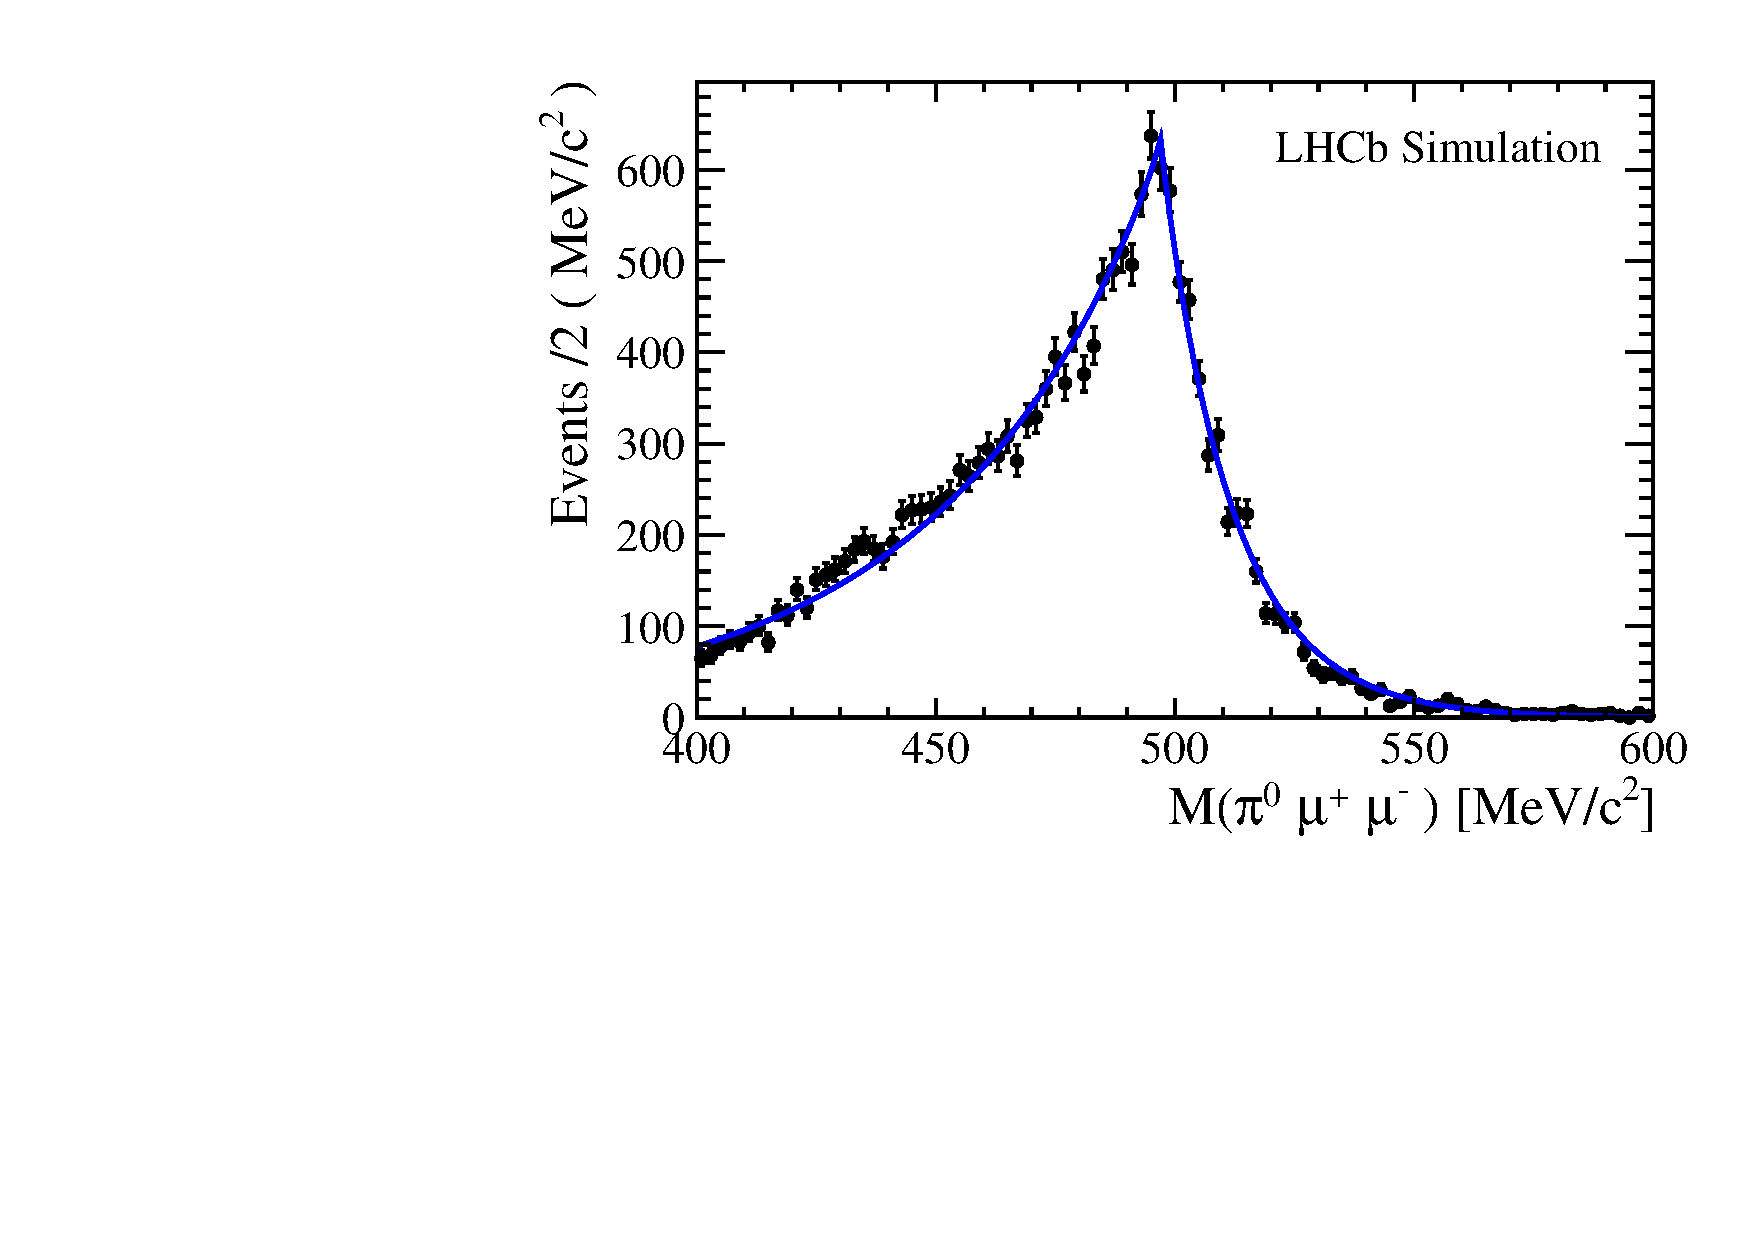
\includegraphics[scale=0.30]{figs/Kspi0MuMu/Ipatia_nopi0.pdf}
\caption{Signal fit using the Hypathia function for FULL (left) and PARTIAL (right) categories. \label{fig:Ipatia}}
\end{center}
\end{figure}

\begin{figure} [htb!]
\begin{center}
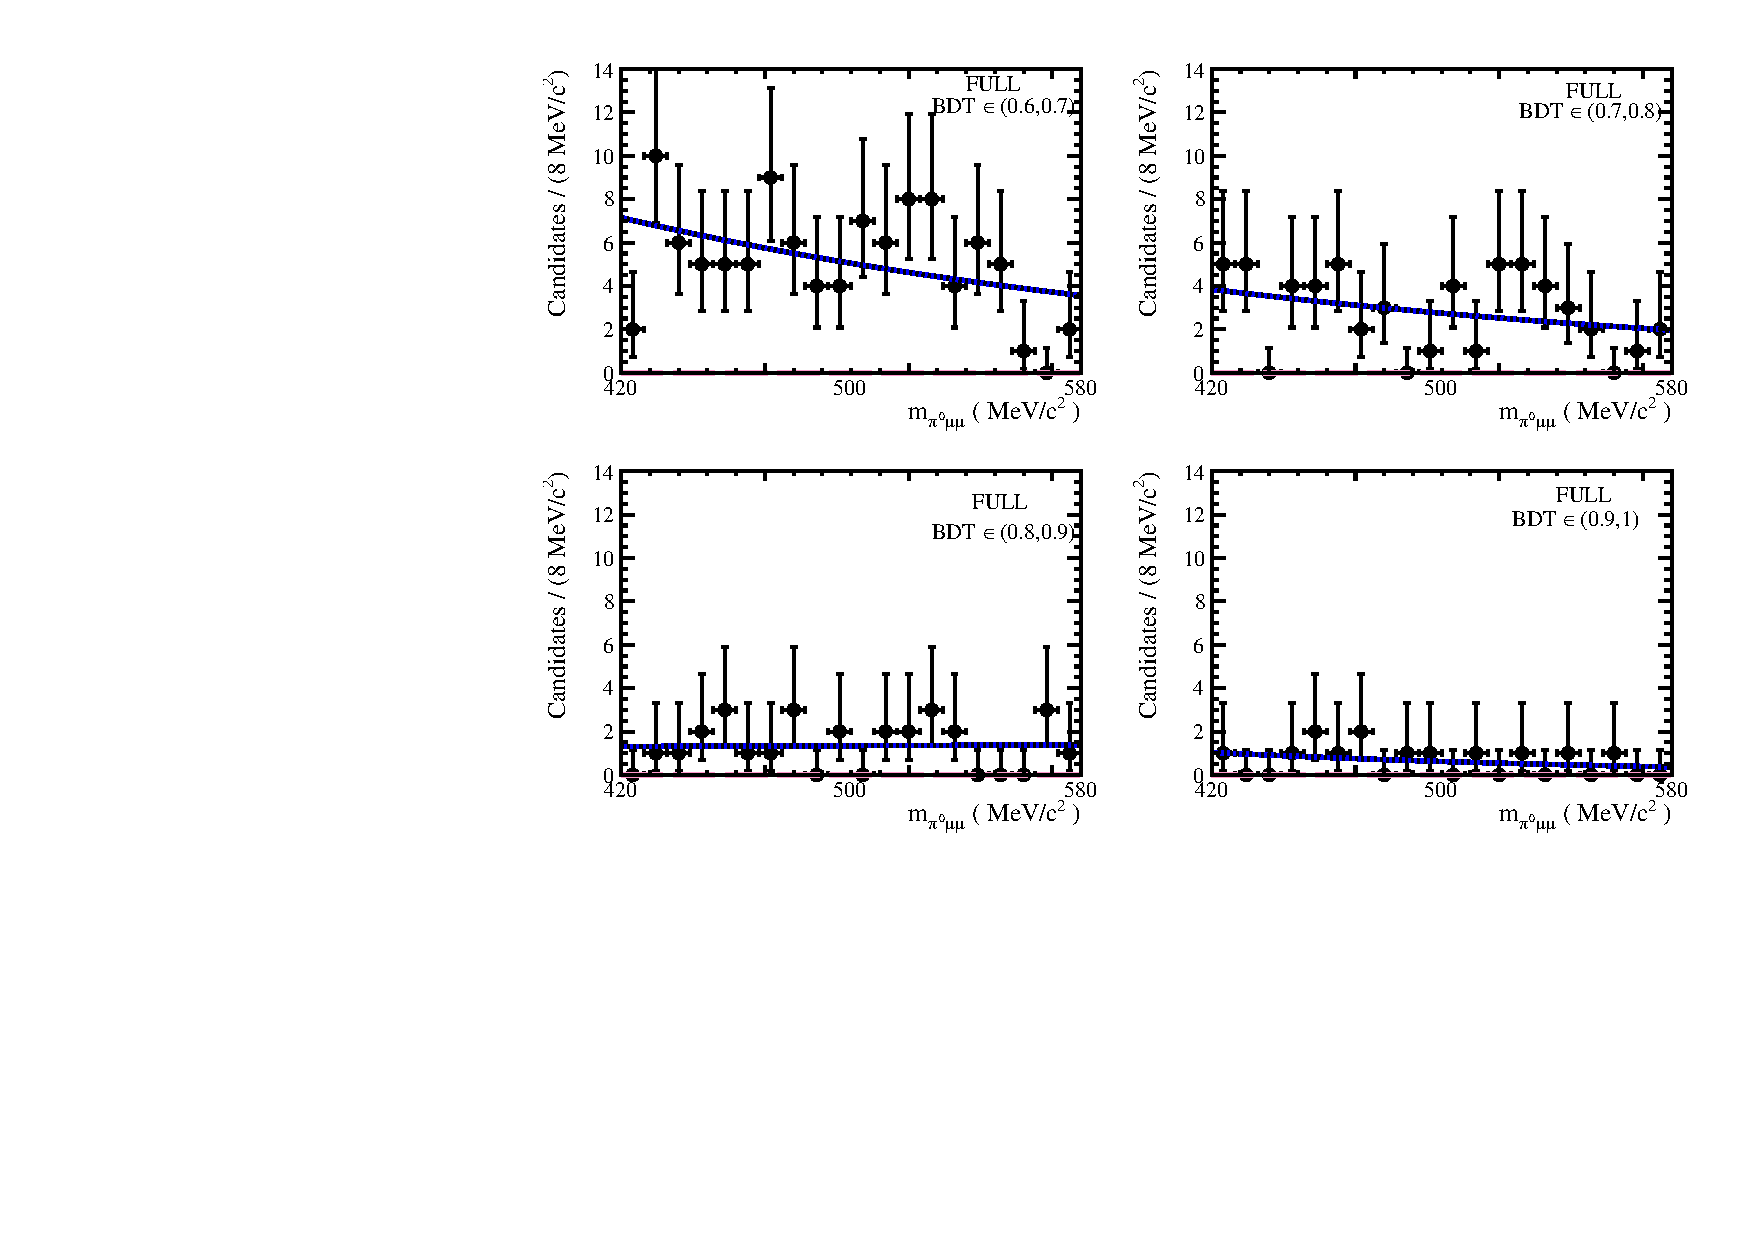
\includegraphics[scale=0.60]{figs/Kspi0MuMu/fit_FULL.pdf}
%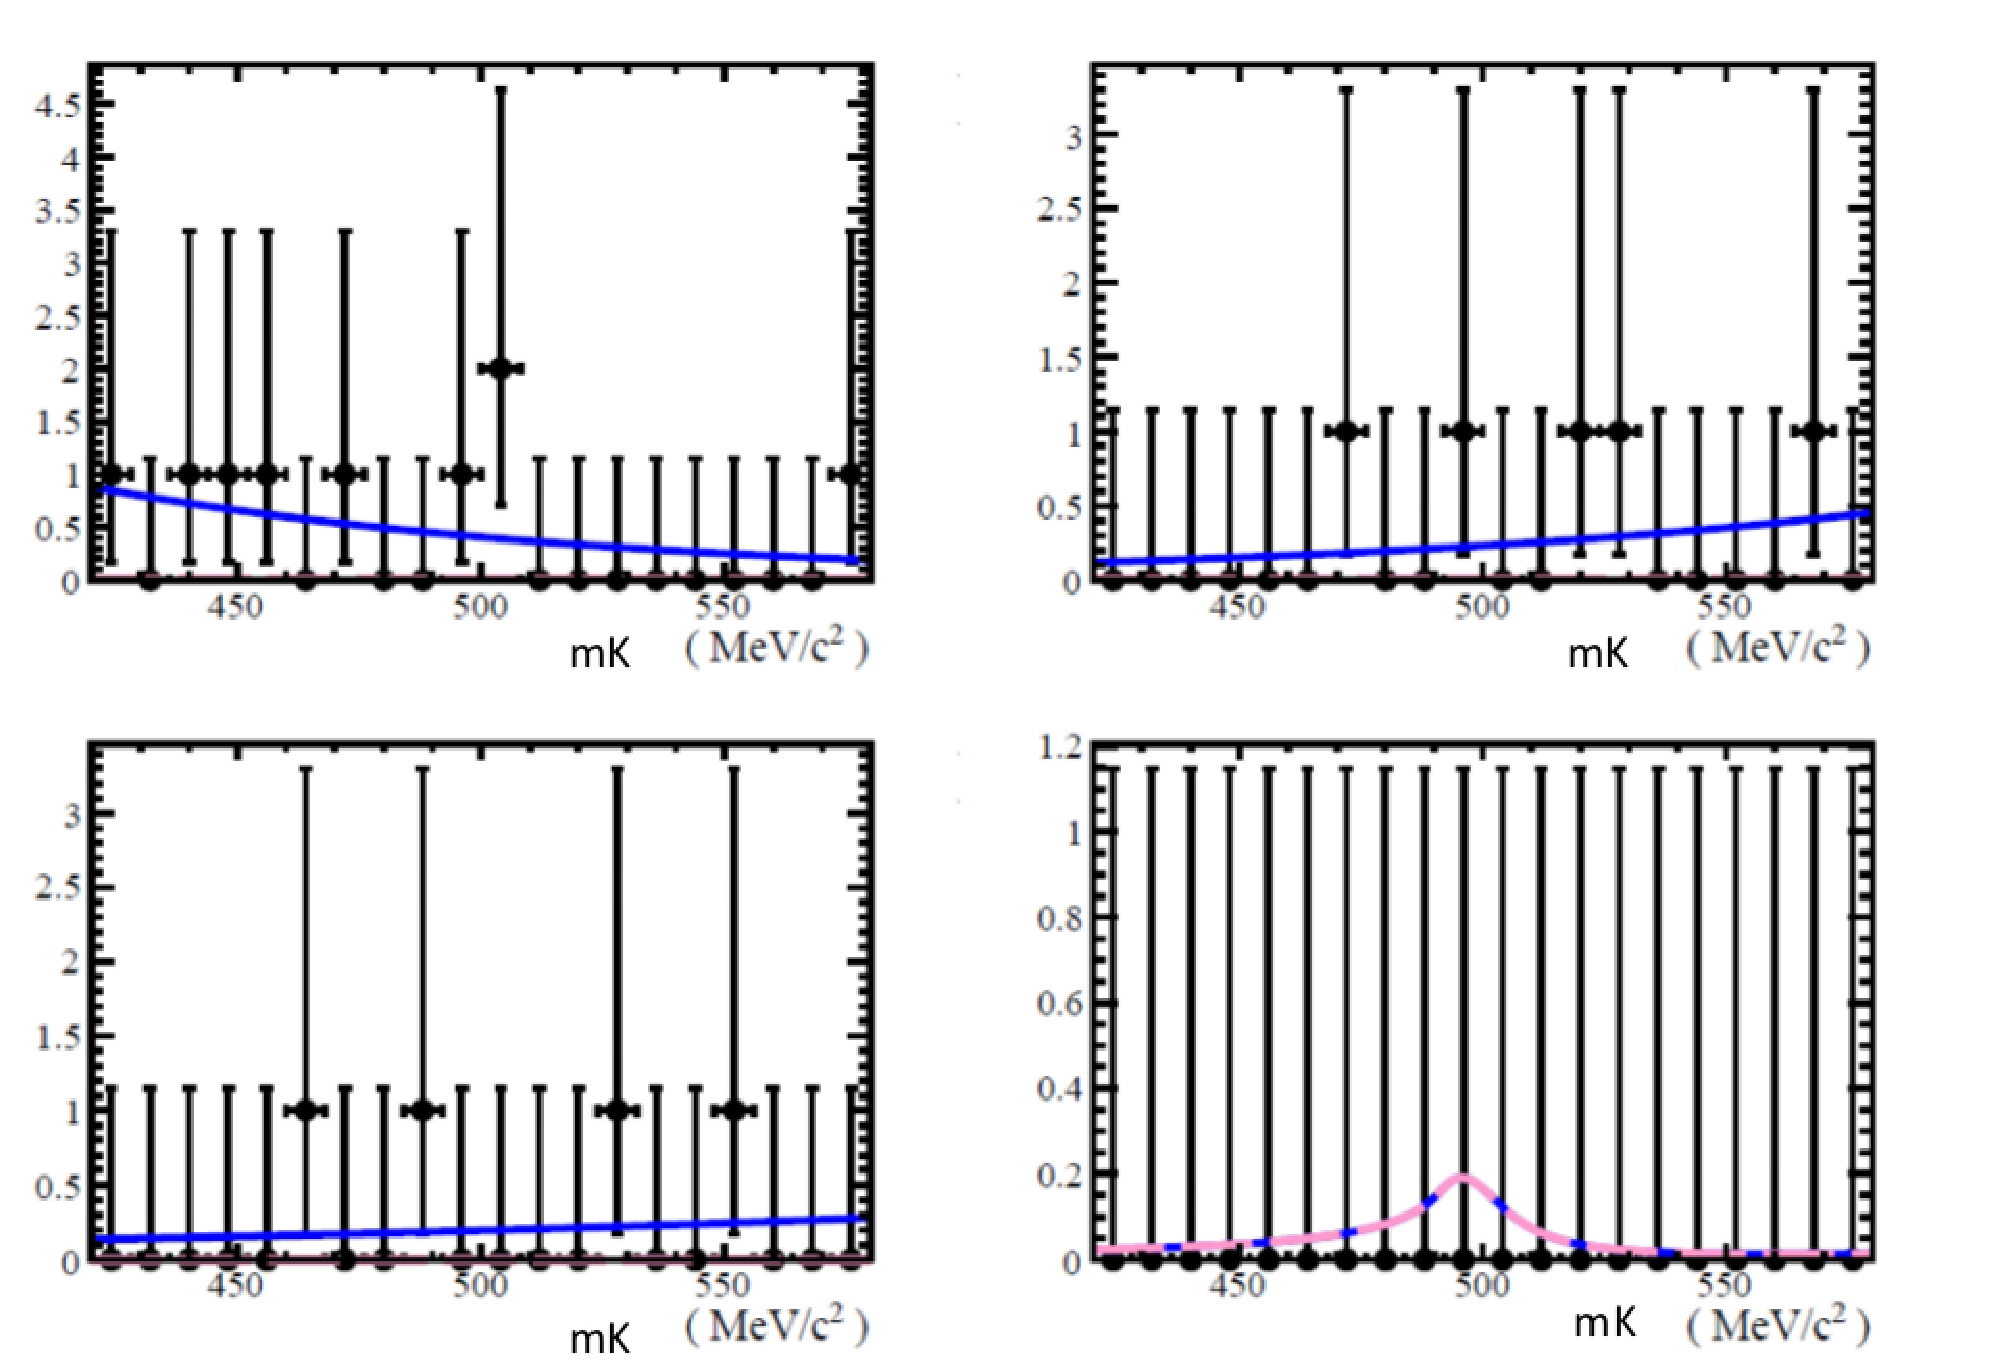
\includegraphics[scale=0.20]{figs/fit_15.pdf}
\includegraphics[scale=0.60]{figs/Kspi0MuMu/fit_PARTIAL.pdf}

\caption{Fit to data for FULL (top) and PARTIAL (bottom) categories. The magenta dashed line shows the signal contribution, the dotted black line the background, and the solid blue line the prediction from the total fit
model.
\label{fig:fit}}
\end{center}

\end{figure}

%\begin{figure} [htb!]
%\begin{center}
%%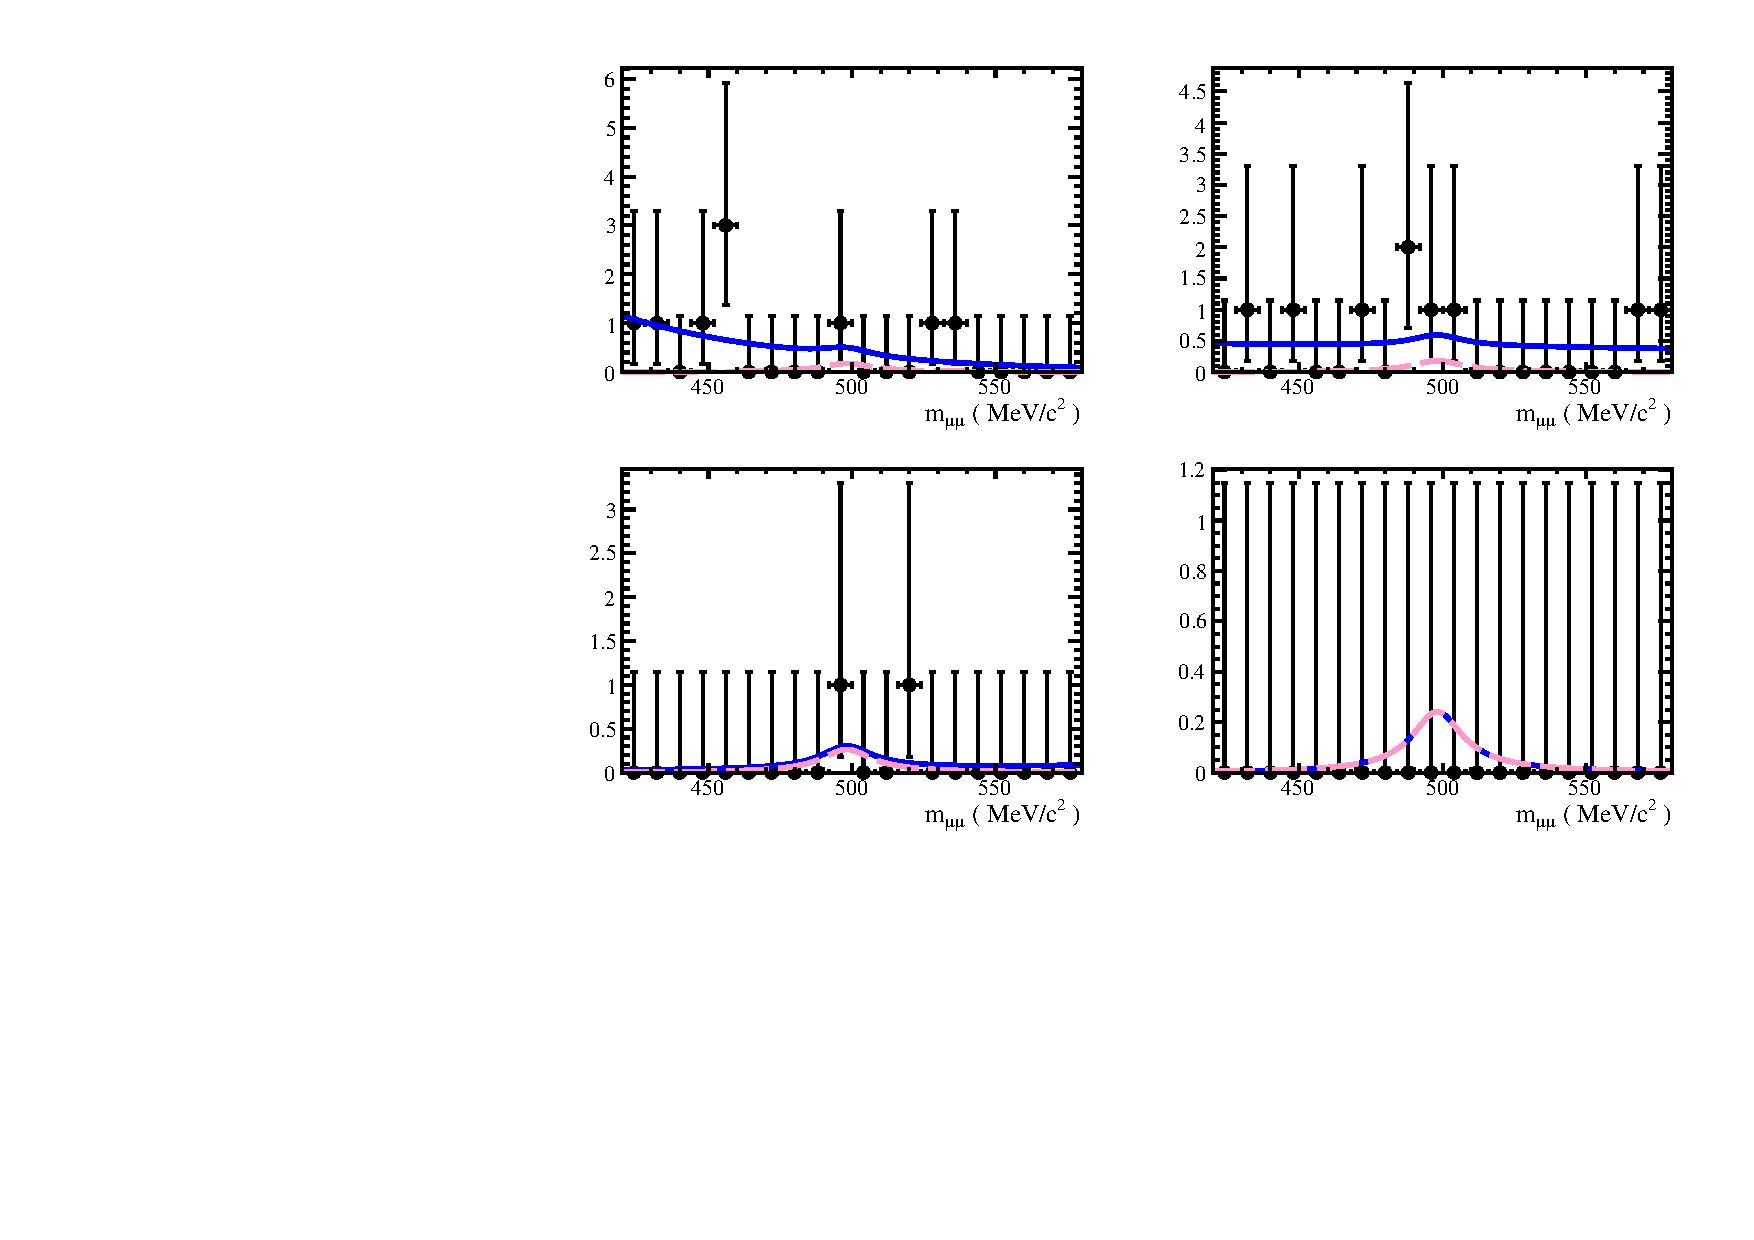
\includegraphics[scale=0.60]{figs/fit_kpmm.pdf}
%\includegraphics[scale=0.60]{figs/fit_PARTIAL.pdf}
%\caption{Fit to data for PARTIAL category. \label{fig:fitPARTIAL}}
%\end{center}
%\end{figure}


%\begin{itemize}
%\item For FULL, we find that the peak shape can be effectively described considering only the 
%resolution parameters
%\end{itemize}

% $Id: introduction.tex 87303 2016-02-08 13:44:29Z lafferty $
\subsection{Expected sensitivity}
\label{subsec:sensitivity}

The expected statistical precision on \BRof\Kspizmm for multiple values of the integrated luminosity up to 100 \invfb is estimated in this section.
% The fit to the available data performed in \secref{sec:fit} allows obtaining the model parameters of the background. 
The TIS samples used are equivalent to a 100\% trigger efficiency sample with an integrated luminosity of 4.9 and 0.77 \invpb for the FULL  and PARTIAL samples, respectively. %This effective luminosity, $L_{eff}^{dat}$, 
%has been estimated using the \Kspipi decays present in the sample, as well as the \Kspipi TIS efficiency, which is $\approx2\times10^{-3}$ as measured using the TISTOS method~\cite{TISTOS}.
The expected background yield is extrapolated from the current data fit result, where the signal yield is consitent with zero.
The background yield is scaled linearly for larger integrated luminosities.
%\begin{equation}
%N_{bkg}^L = N_{bkg}^{dat}\times\frac{L}{L_{eff}^{dat}}.
%\end{equation}

For each integrated luminosity in the studied range, sets of pseudo-experiments are generated  with the above background expectations,
and with a signal yield expectation of
\begin{equation} 
N_{sig} = \frac{\BRof\Kspizmm}{\BRof\Kspipi} \frac{\epsilon_{\KsPzMuMu}}{\epsilon_{\PKzS\to\Pgpp\Pgpm}}  N(\Kspipi)\times \frac{L_{fut}}{L_{curr}},
\end{equation} %dropped NA48 subindex for BR
% % where $\epsilon$ is the corresponding detection efficiency and 
where $L_{fut}$ and $L_{curr}$ are the future and current luminosities, respectively.
The models described in \secref{subsec:fit} are fit to each pseudo-experiment with a floating \BRof\Kspizmm.
The background model parameters used are the ones obtained from the fit to the data \secref{subsec:fit}. The statistical uncertainties
are obtained as the variations of \BRof\Kspizmm that deviate from the minimum of the log-likelihood profile by half a unit.
Finally, the uncertainties are averaged across the set of pseudo-experiments for a given integrated luminosity.
The uncertainties on the background extrapolation are large and translate into large uncertainties on the luminosity needed for achieving a given sensitivity. The resulting sensitivity curves are shown
in \figref{fig:sensitivity}.
It can be seen that the analyses of both PARTIAL and FULL categories can lead to a precision
better than NA48 for the LHCb upgrade if a trigger efficiency above $\approx 50\%$ can be maintained. The \KS production cross-section increases by $\approx20\%$ at 14 $\rm TeV$ compared to 8 $\rm TeV$, but this increase is cancelled by a 
larger fraction of \KS decaying outside of the VELO volume. For this reason, no energy correction has been applied to the sensitivity estimate.
Studies of \Kspizmm and minimum bias samples simulated with the LHCb upgrade detector and conditions show that the High Level
Trigger rate can be kept low enough for a 100 \% efficiency. Further timing studies are currently ongoing.


\begin{figure} [htb!]
\begin{center}
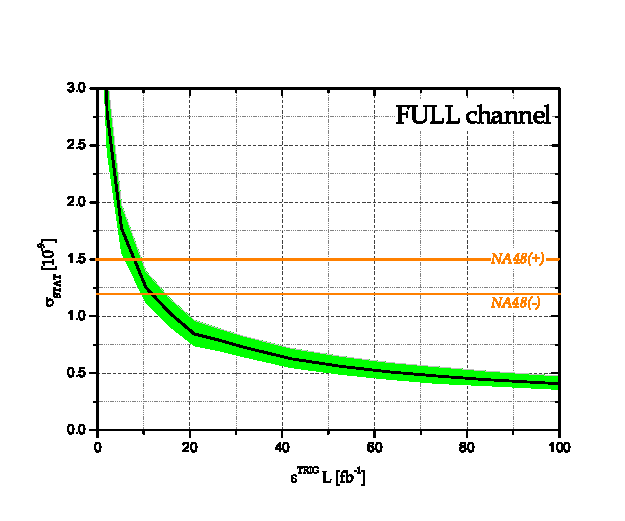
\includegraphics[scale=0.80]{figs/Kspi0MuMu/sensit_FULL.pdf}%{figs/sensitivity_more_colorfull.pdf}
\includegraphics[scale=0.80]{figs/Kspi0MuMu/sensitPARTIAL.pdf}
%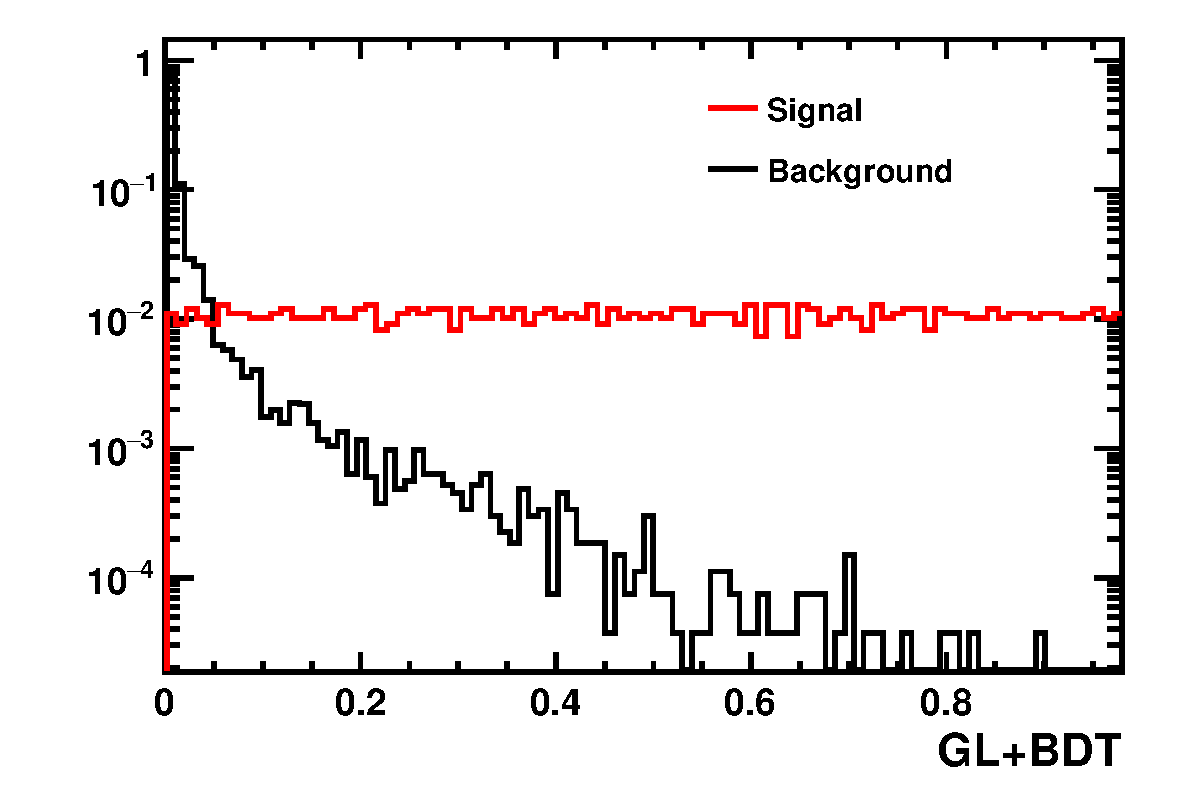
\includegraphics[scale=0.30]{figs/bdt_partial.pdf}
\caption{Expected precision on \BRof\Kspizmm for the FULL (top) and PARTIAL (bottom) channels, as a function of the integrated luminosity times trigger efficiency, $L\times\varepsilon^{TRIG/SEL}$. \label{fig:sensitivity}}
%The green line indicates the behavior of the precision extrapolating from the best fit value of the expected background. In the case of the black curve, this extrapolation is done averaging the background predictions within their uncertainties, while in the orange case the extrapolation takes as reference the best fit value of the expected background deviated one sigma from its mean value. \label{fig:sensitivity}}
\end{center}
\end{figure}


%\begin{figure} [htb!]
%\begin{center}
%\includegraphics[scale=0.60]{figs/sensitPARTIAL.pdf}
%%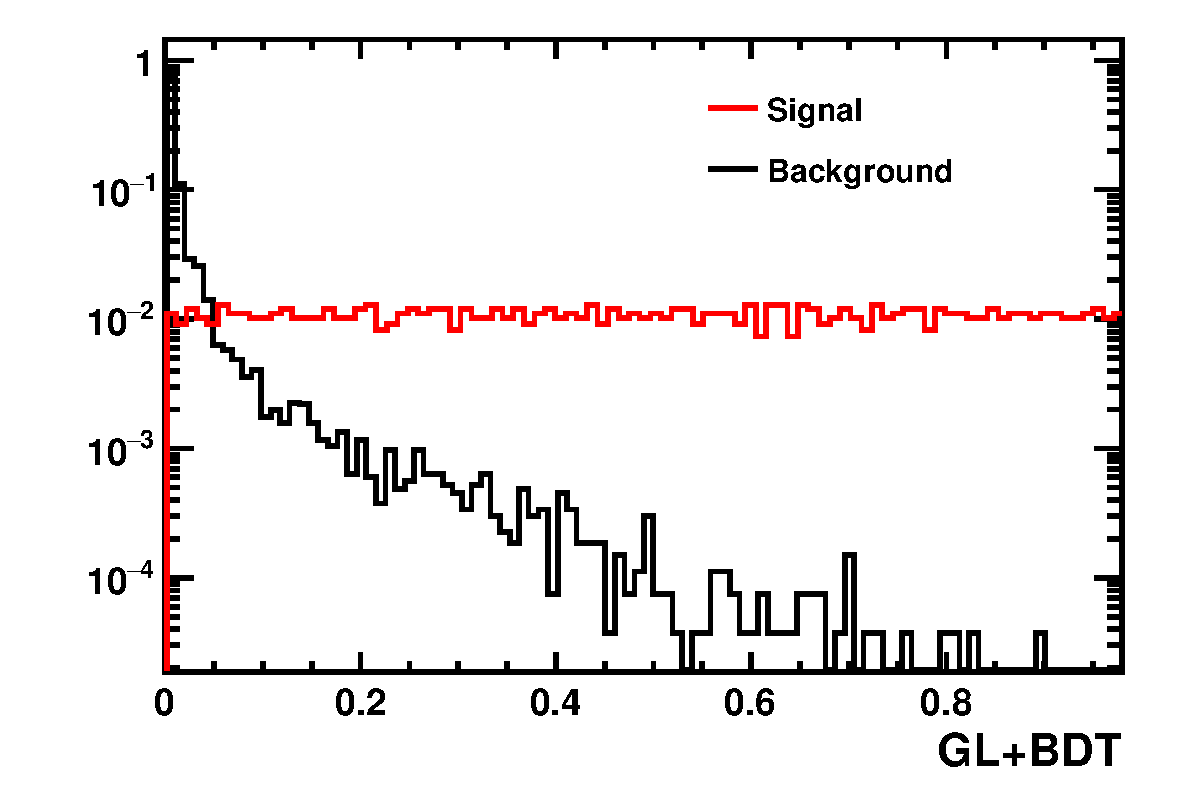
\includegraphics[scale=0.30]{figs/bdt_partial.pdf}
%\caption{Expected precision on \BRof\Kspizmm for the PARTIAL channel, as a function of the integrated luminosity times trigger efficiency, $L\times\varepsilon^{TRIG/SEL}$. The green 
%line indicates the behavior of the precision extrapolating from the best fit value of the expected background. In the case of the black curve, this extrapolation is done averaging the background 
%predictions within their uncertainties, while in the orange case the extrapolation takes as reference the best fit value of the expected background deviated one sigma from its mean value. {\it some lines are actually not there , but the plot in general needs to
%be updated} \label{fig:sensitivityPARTIAL}}
%\end{center}
%\end{figure}





 


% $Id: introduction.tex 87303 2016-02-08 13:44:29Z lafferty $

\subsection{Conclusions}
\label{subsec:conclusions}
A precise measurement of the \Kspizmm branching fraction is crucial for a precise ${\cal B}(\PKzL\to\Pgpz\APmuon\Pmuon)$ SM theoretical prediction and the search for physics beyond the SM in ${\PKzL}\to\Pgpz\APmuon\Pmuon$.
The sensitivity of the LHCb experiment to \BRof\Kspizmm was studied based on $3\;\rm fb^{-1}$ of data recorded at 7 and $8\;\rm TeV$ center-of-mass energy during 2011 and 2012, and on $0.3\;\rm fb^{-1}$ 
of data recorded at $13\;\rm TeV$ center-of-mass energy during 2016. Full and partial decay reconstruction algorithms were considered, aiming at 
a high reconstruction efficiency. The sensitivity study was performed using pseudo-experiments by extrapolating signal yield results based on the currently available data to expected future integrated luminosities.
If a trigger efficiency of at least 50\% can be assured in the future, LHCb can determine \BRof\Kspizmm with a precision significantly better than that of NA48.
%up to almost $10^{-10}$, which would be an improvement by an
%{\it We are the champions}


%% $Id: introduction.tex 87303 2016-02-08 13:44:29Z lafferty $
\clearpage
\newpage
\section{Appendix: Selection and BDT}
\label{app:selection}
%{\it Fill in the details of the stripping selection, fiducial cuts
%and BDT (RoC curves, signal and backgroung histrograms of input variables ...)}

% Stripping selections

The stripping selection lines for the \KsPzMuMu and \Kspipi candidates are
\begin{itemize}
 \item StrippingK0s2Pi0MuMuLines: used for the FULL \KsPzMuMu category
 \item TriggerTestLine (in StrippingRareNStrange): used for the PARTIAL \KsPzMuMu category.
\end{itemize}
Both stripping lines use the same selection criteria for \Kspipi. 
%  \item
%  \item
%  \item Daughters must not be compatible with coming directly from the PV, by requiring a high impact parameter $\chi^2$, which is defined as the difference of the $\chi^2$ of the PV fit obtained with and without 
%  the considered track.
The stripping criteria for all lines are summarized in \tabref{stripping:pipi}. They are as follows:
\begin{itemize}
 \item The \Kspipi sample is prescaled by a factor of 0.001 due to its large size.
 \item The charged-particle containers StdAllLooseMuons and StdNoPidsPions are used.
 \item Only resolved $\pi^{0}$ candidates are used, as the merged contribute only with additional 2.9\%.
 \item \KS{}  M: \KS\ candidate mass is required to be in the range [400, 600] \mevcc{} for the FULL and \Kspipi samples.
 \item $\mu^{+}\mu^{-}$  M: The dimuon candidate mass for the PARTIAL sample is required to be smaller than 450 \mevcc to reduce the contribution from misidentified \Kspipi. This is a loose requirement,
       given that the maximum dimuon mass, without considering the detector response, is $m_{\KS}-m_{\pi^{0}}=362$ \mevcc.
 \item \KS{} tof: Proper decay time of the \KS\ candidate given in a fraction of the \KS\ lifetime. This variable is computed using the reconstructed momentum of the \KS candidate and the distance between 
      the reconstructed secondary (SV) and primary (PV) vertices.
 \item \KS{} IP:  The \KS\ candidate must be compatible with the PV, asking for a low impact parameter with respect to PV.
 \item $\mu^{+}\mu^{-}$ DIRA: Forward \KS\ decay, requiring a positive cosine of the polar direction angle (DIRA).
 \item $\mu^{+}\mu^{-}$ DOCA: Good reconstruction quality of the SV required asking for a low distance of closest approach (DOCA) of the two daughter tracks.
 \item Daug. Track $\chi^{2}/ndof$:  Good reconstruction quality of the muon/pion tracks is required using the $\chi^{2}/ndof$ of the track fit. This is the standard cut of long tracks in LHCb.

 \item Daug. IP$_{\chi^{2}}$ : Daughters must not be compatible with coming directly from the PV, by requiring a high impact parameter $\chi^{2}$, which is defined as the difference of the $\chi^{2}$ of the PV
       fit obtained with and without the considered track.
 \item Daug. Track ghost prob.:  accounts for the probability that a track does not correspond to a track from a single charged particle.
 \item Daug. PID: The DLL $\mu-\pi$ ($log(P_{\mu}/P_{pi})$) is used to increase the muon purity at stripping level.
 \item Vertex $\rho$: The radial distance between the dimuon vertex in LHCb coordinates.
 \item Vertex $z$: The distance in $z$ (LHCb coordinates).
 \item Vertex $\chi^{2}/ndof$: A good-quality vertex is assured by placing a requirement on its fit quality.
 \item $\delta_{z}$: Distance from the end vertex of the particle and the related primary vertex.
 \item $\cos\alpha$: Cosine of the angle between the \KS\ momentum and the direction fo flight from the best PV to the decay vertex.
 \item IP$_{\text{max}}$/$\delta_{z}$.
\end{itemize}

\begin{table}[!ht]
\centering
\begin{tabular}{l@{\hspace{0.5cm}}l@{\hspace{0.5cm}}l@{\hspace{0.5cm}}l}
\hline
\textbf{Variables}                & $\boldsymbol{\Kspizmm}$ & $\boldsymbol{\Kspizmm}$ &$\boldsymbol{\Kspipi}$  \\
				  & {\bf FULL} &  {\bf PARTIAL} &  \\
\hline
Stripping line			  & K0s2Pi0MuMuLines & TriggerTestLine & K0s2Pi0MuMuLines\\
			          & & & RareNStrange\\
Prescale			  & 1 & 1 & 0.001\\
Input Particles              	  & StdAllLooseMuons & StdAllLooseMuons & StdNoPidsPions   \\
                                  & StdLooseResolvedPi0 & &   \\
\KS{}  M                          & [400, 600] \mevcc{}  & - & [400, 600] \mevcc{}    \\
$\mu^{+}\mu^{-}$  M               & -  & $<$ 450 \mevcc{} &     \\
\KS{}  tof                        & $>$ 0.06$\tau$ & $>$ 0.06$\tau$ & $>$ 0.1$\tau$  \\
\KS{}  IP                         & $< 0.9$ \small mm &  - & $< 0.4$ \small mm    \\
$\mu^{+}\mu^{-}$ DIRA             & $>$ 0 \small s & $>$ 0  \small s &  $>$ 0  \small s\\
$\mu^{+}\mu^{-}$ DOCA            & $<$ 0.3 \small mm  & $<$ 0.1 \small mm  &  $<$ 0.3 \small mm     \\
Daug. Track $\chi^{2}/ndof$   	  & $<$ 5 & $<$5 &  $<$ 5          \\
Daug. IP$_{\chi^{2}}$         	  & $>$ 36 & $>$ 60 &  $>$ 100        \\
Daug. Track ghost prob.        	  & - & $<$ 0.1 &  -        \\
Daug. PID        	  	  & - & $>$ 0 &  -        \\
Vertex $\rho$        	  	  & - & $>$ 4 \small mm&  -        \\
Vertex $z$        	  	  & - & $>$ 650 \small mm &  -        \\
Vertex $\chi^{2}/ndof$        	  	  & - & $<$ 9 &  -        \\
$\delta_{z}$    		  & - & $>$ 0 \small mm &  -        \\
$\cos\alpha$    		  & - & $>$ 0  &  -        \\
IP$_{\text{max}}$/$\delta_{z}$    & - & $<$ 1/60 s$^{-1}$&  -        \\
\hline
\end{tabular}
\caption[Stripping selection]{The \Kspizmm and \Kspipi selection cuts performed in the stripping phase.
The definitions of the variables is given in the text.}
\label{stripping:pipi}
\end{table}

The candidates were selected using three Strippings: 
\begin{itemize}
\item Stripping 21: used for 2011/2012 data
% \item Stripping 24: used for 2015 data
\item Stripping 26: used for 2016 data.
\end{itemize}

The PARTIAL analisys is tested in Stp26, while the FULL is tested in Stp21.
% BDT  (variables, RoC curves, signal and background histograms of input variables)

Before the training, the following cuts are made on the data to reduce the amount of background (while keeping most of the signal):
\begin{itemize}
\item Number of hits in the Trigger Tracker greater than 0.1 for both muons
\item ProbNNmu greater than 0.05 
\item Lifetime of the \KS greater than 1 ps
\item Invariant mass of the decay result smaller than 490 \mev
\item Kinematic cut in the Armenteros-Podolanski plane, removing $\Lambda\to p \pi$ and $\KS\to \pi^{+}\pi^{-}$ 
\end{itemize}
The input MVA variables used are divided into continuous variables and discrete variables. The continuous variables are gaussianized, decorrelated, and gaussianized again. Then the gaussianized and the discrete 
variables are inputs for the BDT training. 
% {\it put table with cuts and values, as well as names of the containers of the input particles}
The set of variables common to the FULL and PARTIAL cases consists of:
\begin{itemize}
\item Distance of closest approach (DOCA)
\item \KS flight distance significance. 
\item $\chi^2$ of $\mu$ track fit
%\item Muon impact parameter
\item Vertex $\chi^2$
%\item ProbNNmu: probability for the muon to be a real muon instead of another particle
\item \KS $p_T$ 
\item \KS impact parameter significance (difference in the $\chi^2$ of the fit of the vertex obtained with and without the introduction of the track in the fit)
\item Impact parameter significance of the muons with respect to any PV in the event
\item PID variables for muons
\end{itemize}


\begin{itemize}
\item Hits in VELO 
\item Hits in Inner Tracker
\item Hits in Trigger Tracker
\item Hits in Outer Tracker
\item Secondary Vertex coordinates 
\end{itemize}

Apart from these, there are inputs that are specifically used for FULL. \\

\textbf{FULL:}

\begin{itemize} %FULL
\item Angle between $\mu \mu$ and $\gamma\gamma$ planes
\item \Pgpz mass
\item Helicity angles (as defined in \figref{fig:angles}). 
\end{itemize}


\begin{figure} [htb!]
\begin{center}
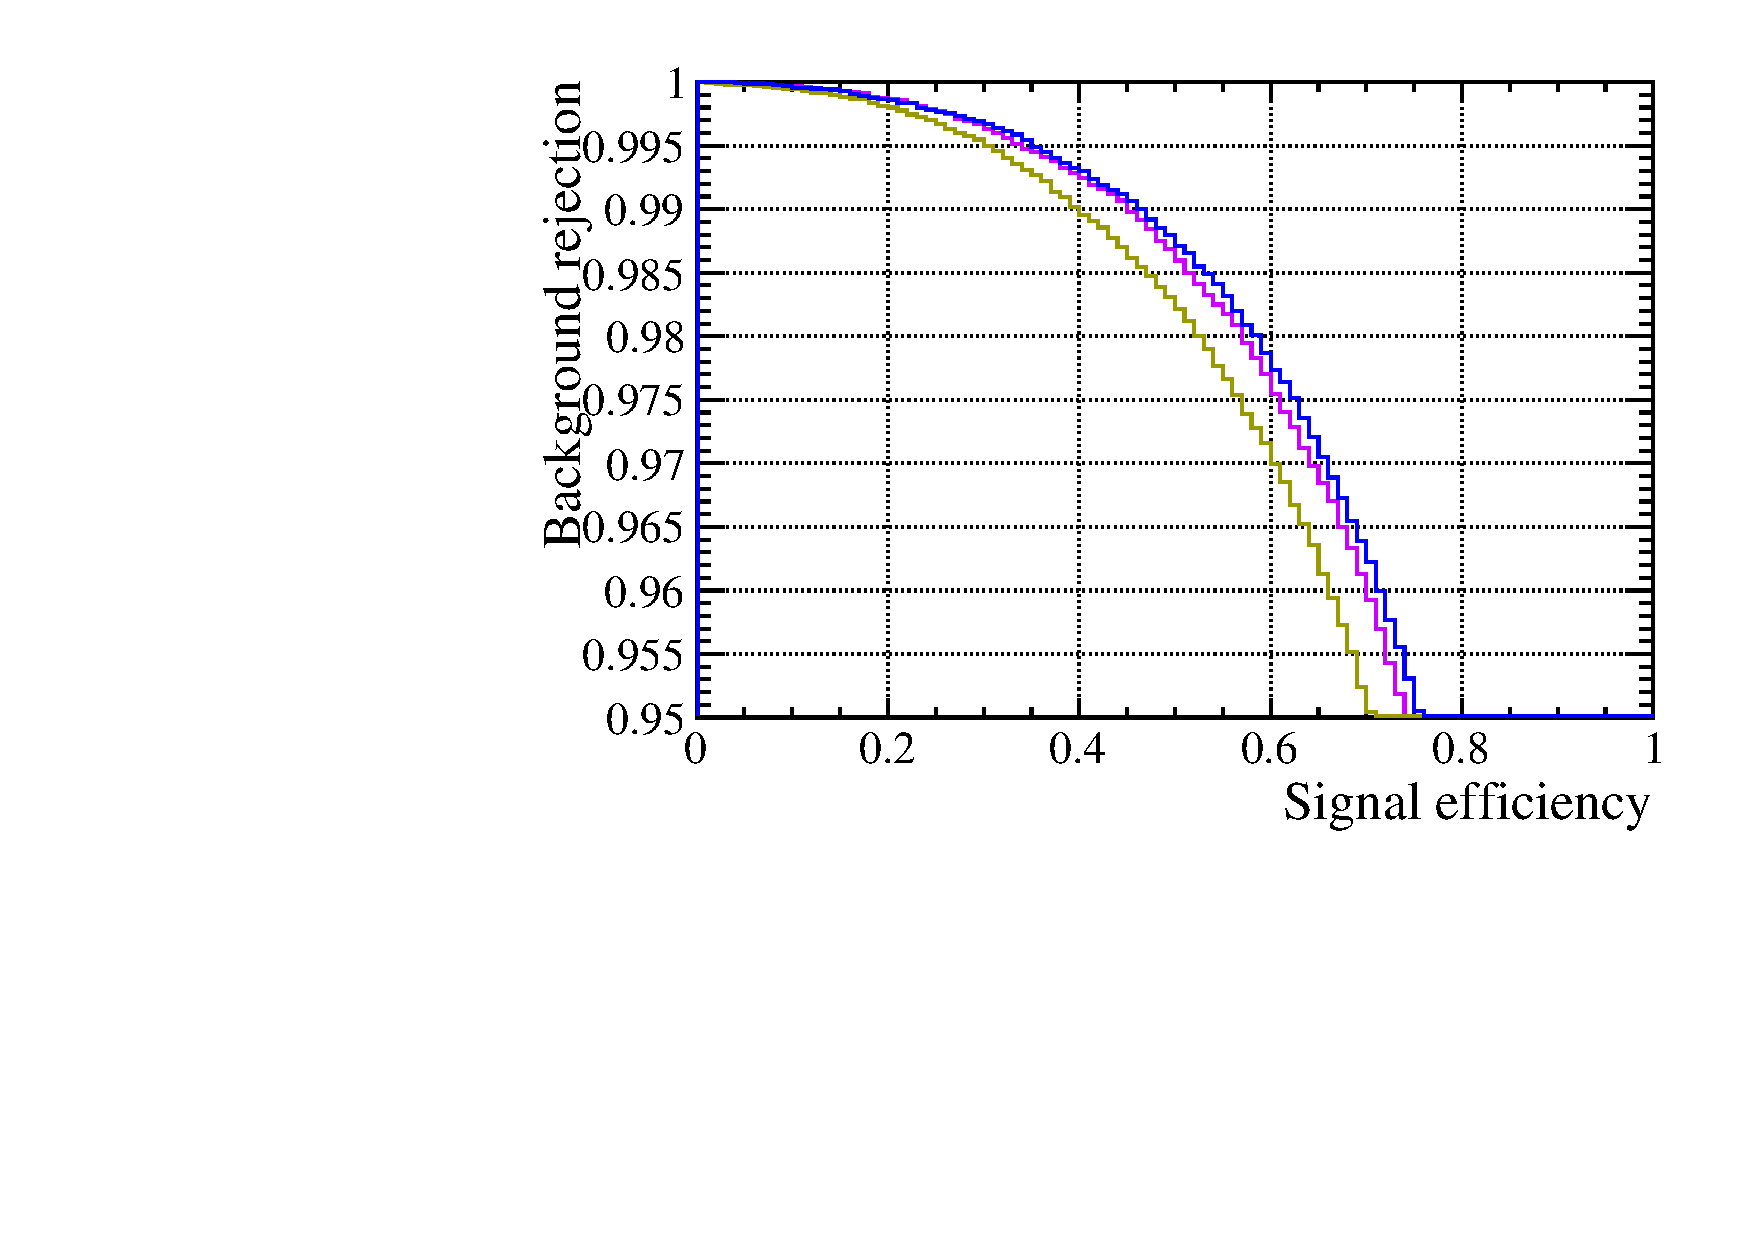
\includegraphics[scale=0.50]{figs/GL_BDT_Kspi0_pi0.pdf}
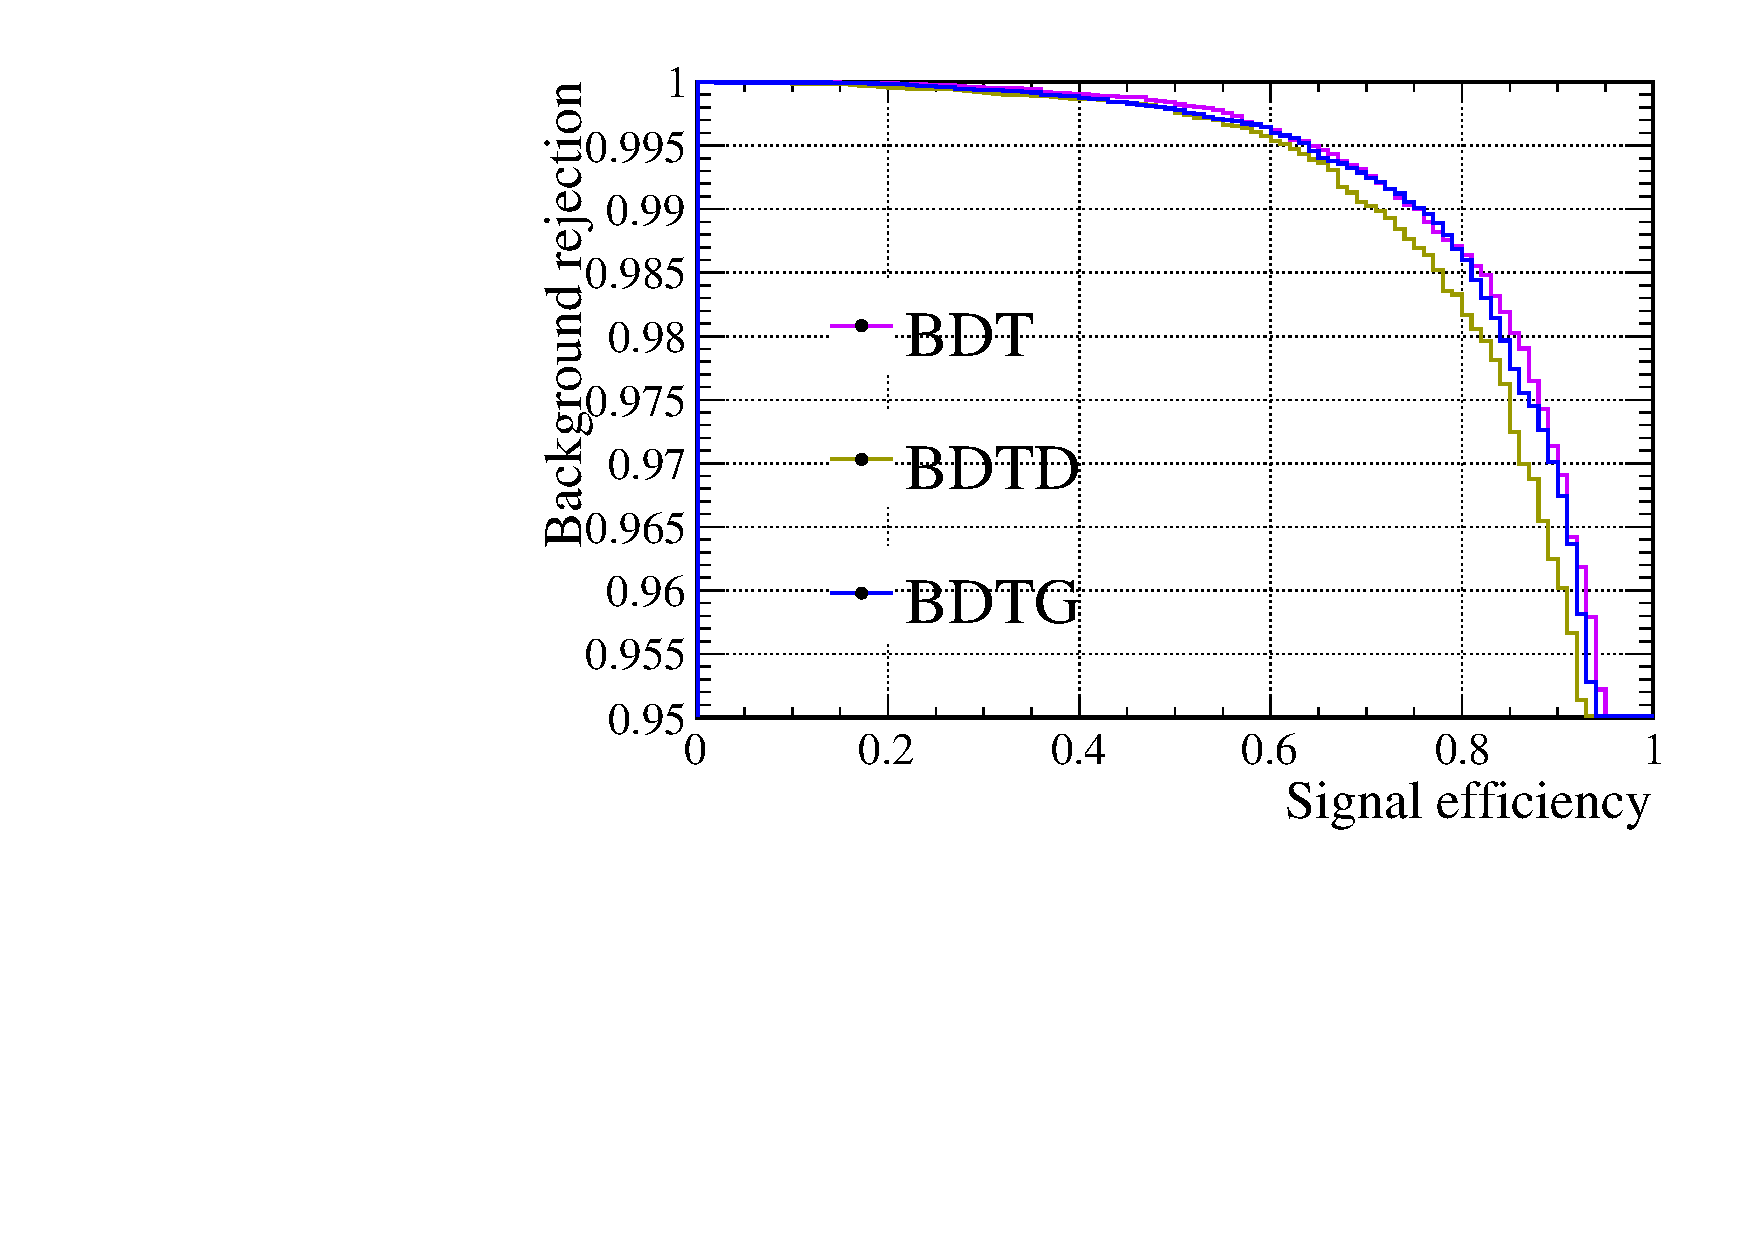
\includegraphics[scale=0.50]{figs/ROC_PARTIAL_noGhost.pdf}%GL_BDT_Kspi0_nopi0_VC.pdf}
\caption{ROC curves for the FULL (top) and PARTIAL (bottom) categories.  \label{fig:ROC}} % TODO \textcolor{red}{Resize, remove BDTB}
\end{center}

\end{figure}

%Signal and background histograms of input variables (plots for input variable distributions)
The ROC (Receiver Operating Characteristic) curves obtained for both cases are represented in \figref{fig:ROC}. 
Finally, in \figref{fig:MVAhistos_FULL1}, \figref{fig:MVAhistos_FULL2} and \figref{fig:MVAhistos_PARTIAL} the histograms for signal and background of the BDT input variable distributions are shown for the 
FULL and PARTIAL categories, respectively. 
We find that the fraction of MC signal \KS coming from $b$ or $c$ decays
is less than a per mil.

\begin{figure} [htb!]
\begin{center}
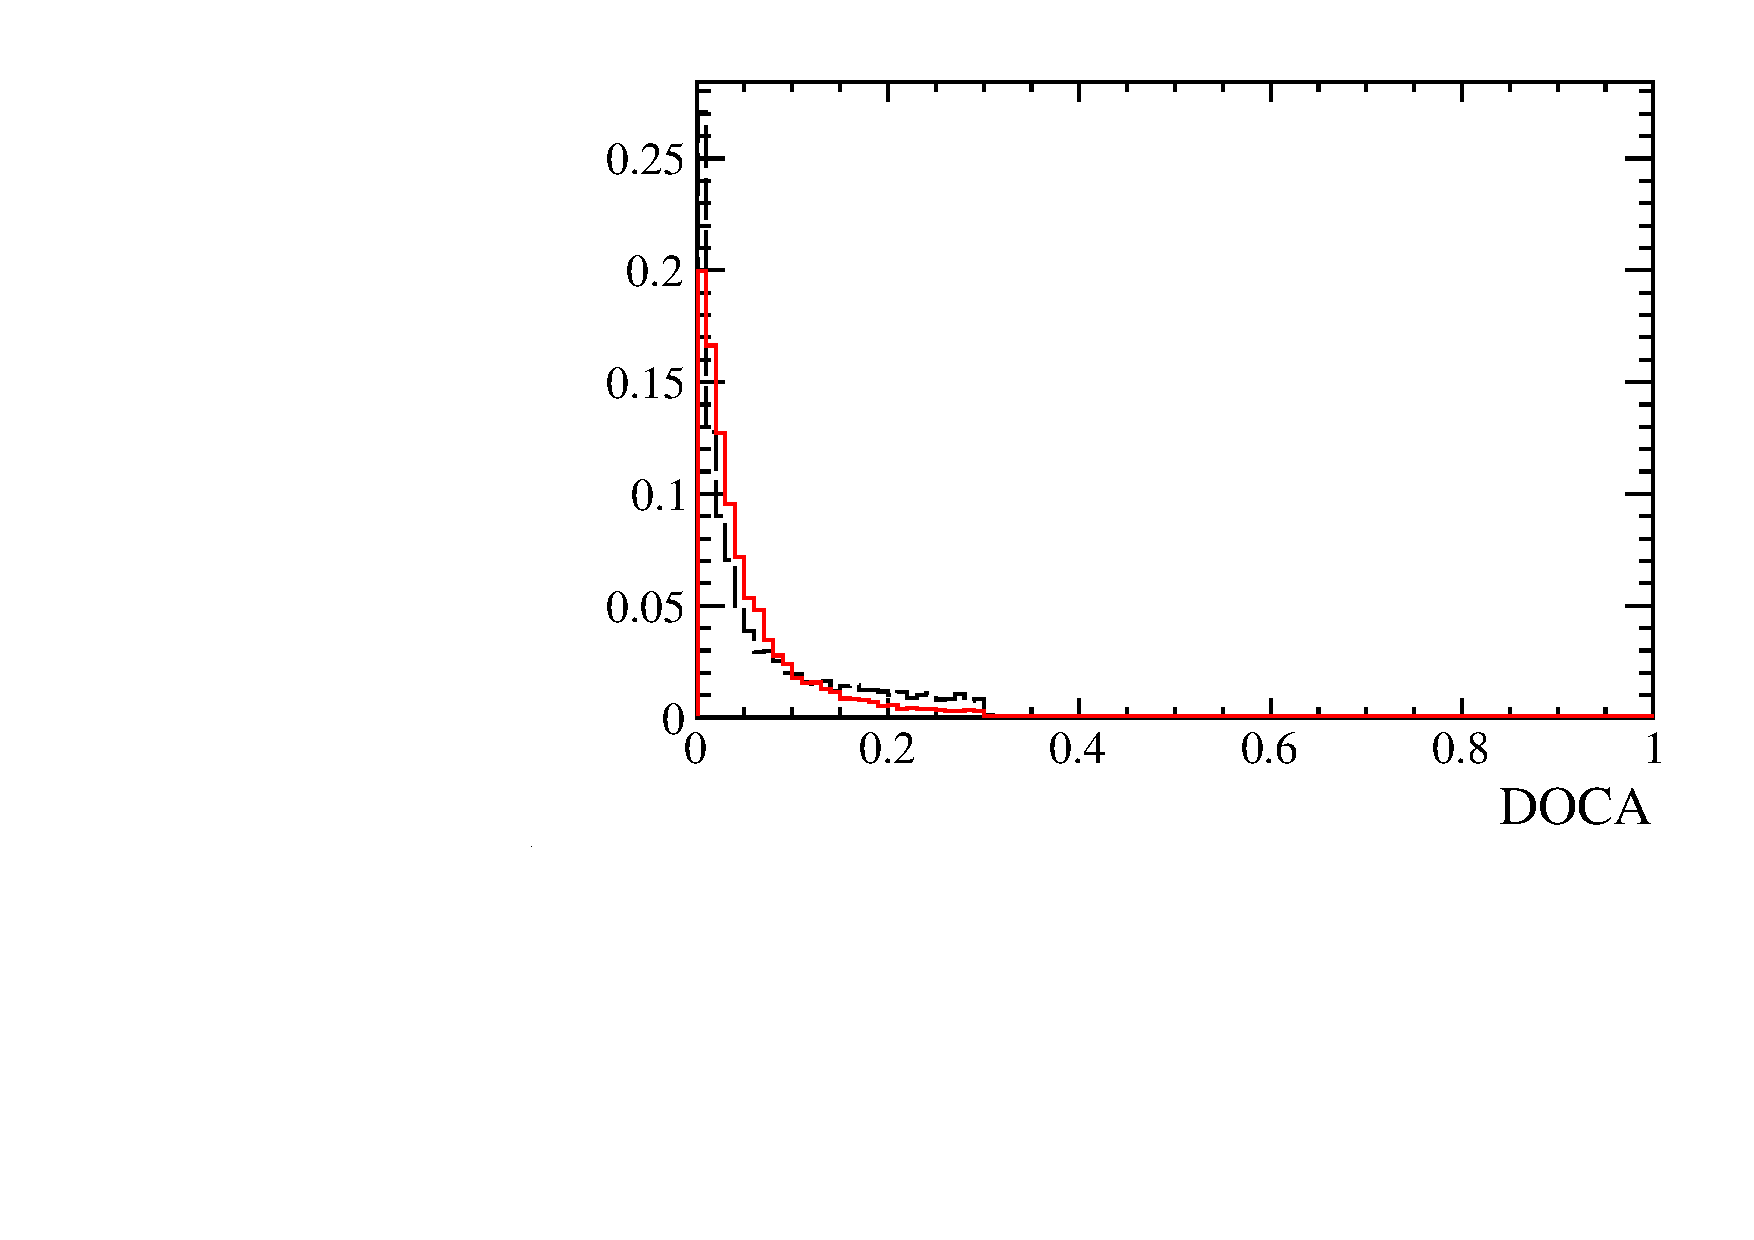
\includegraphics[scale=0.20]{figs/DOCAFULL.pdf}
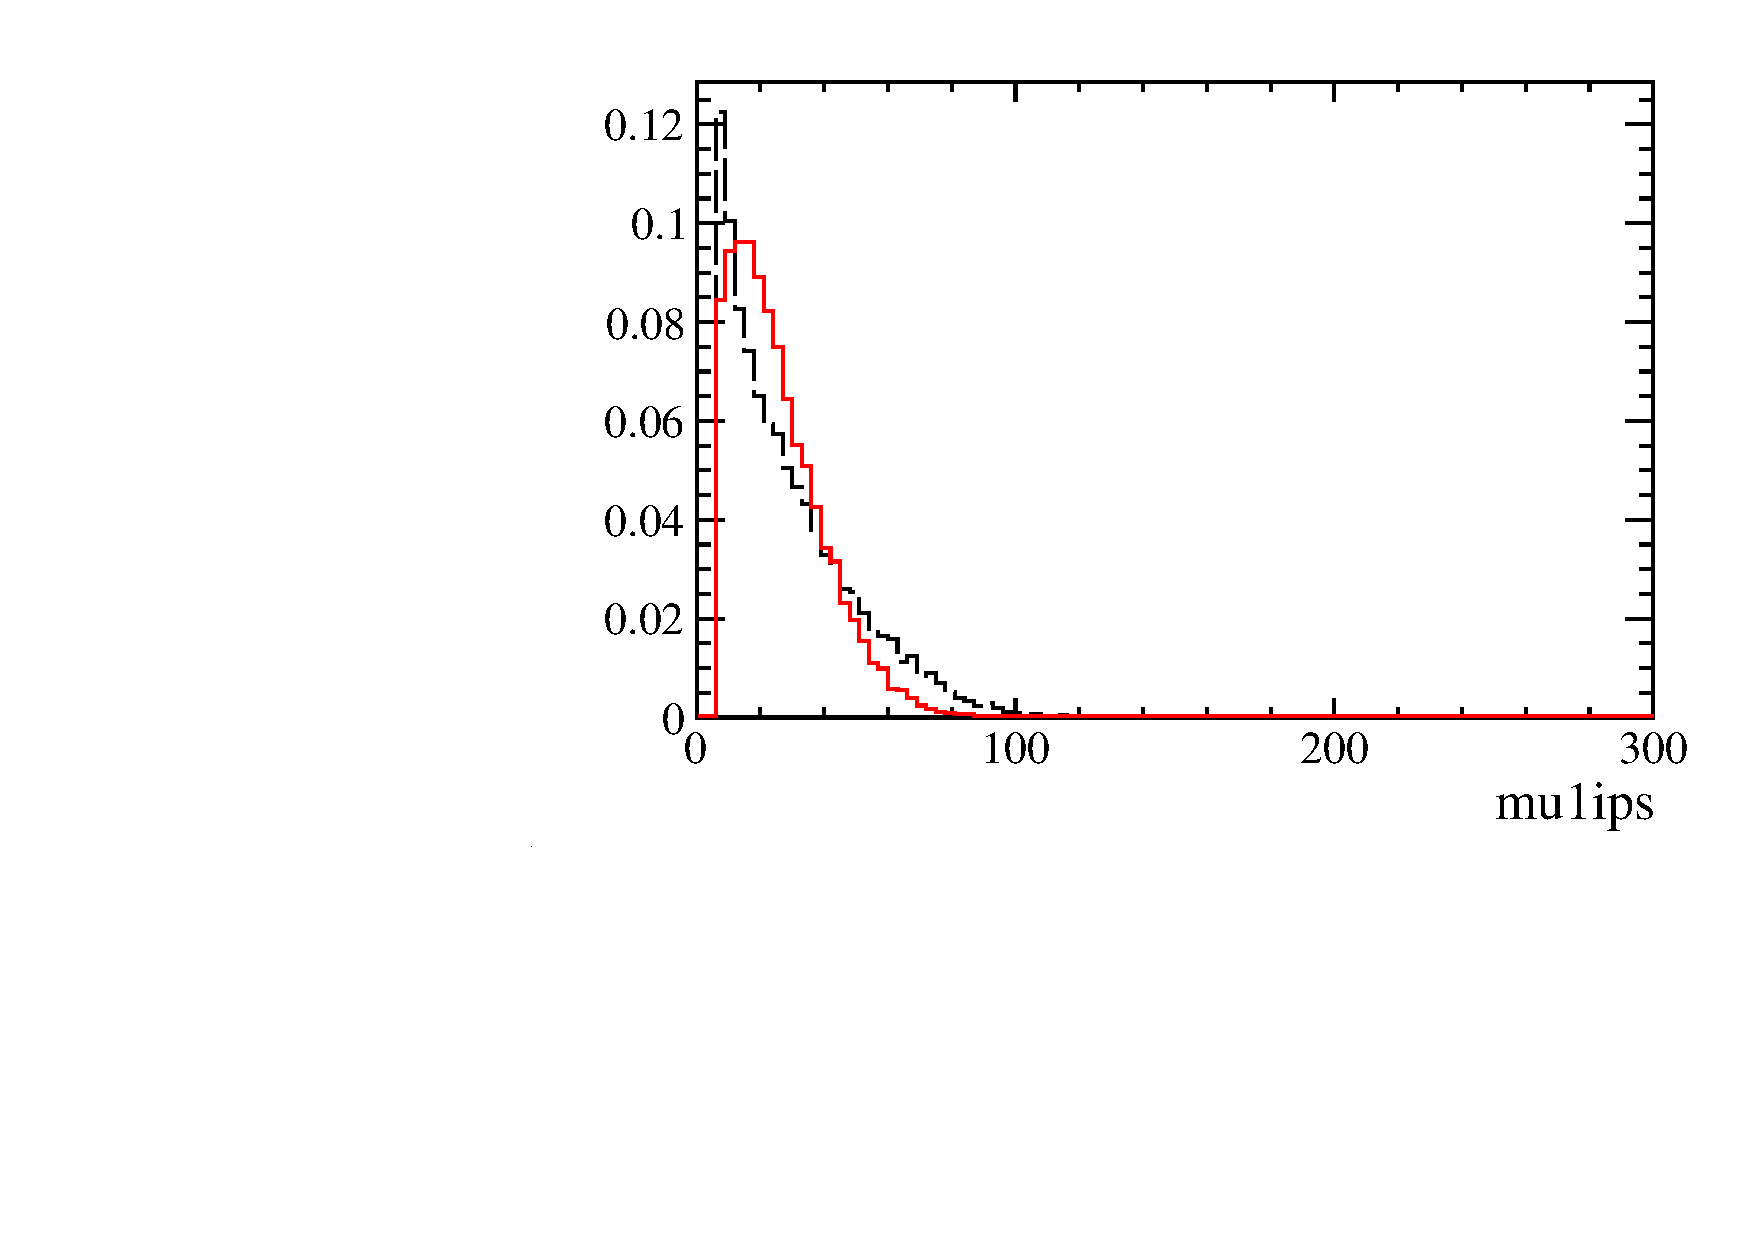
\includegraphics[scale=0.20]{figs/mu1ipsFULL.pdf}
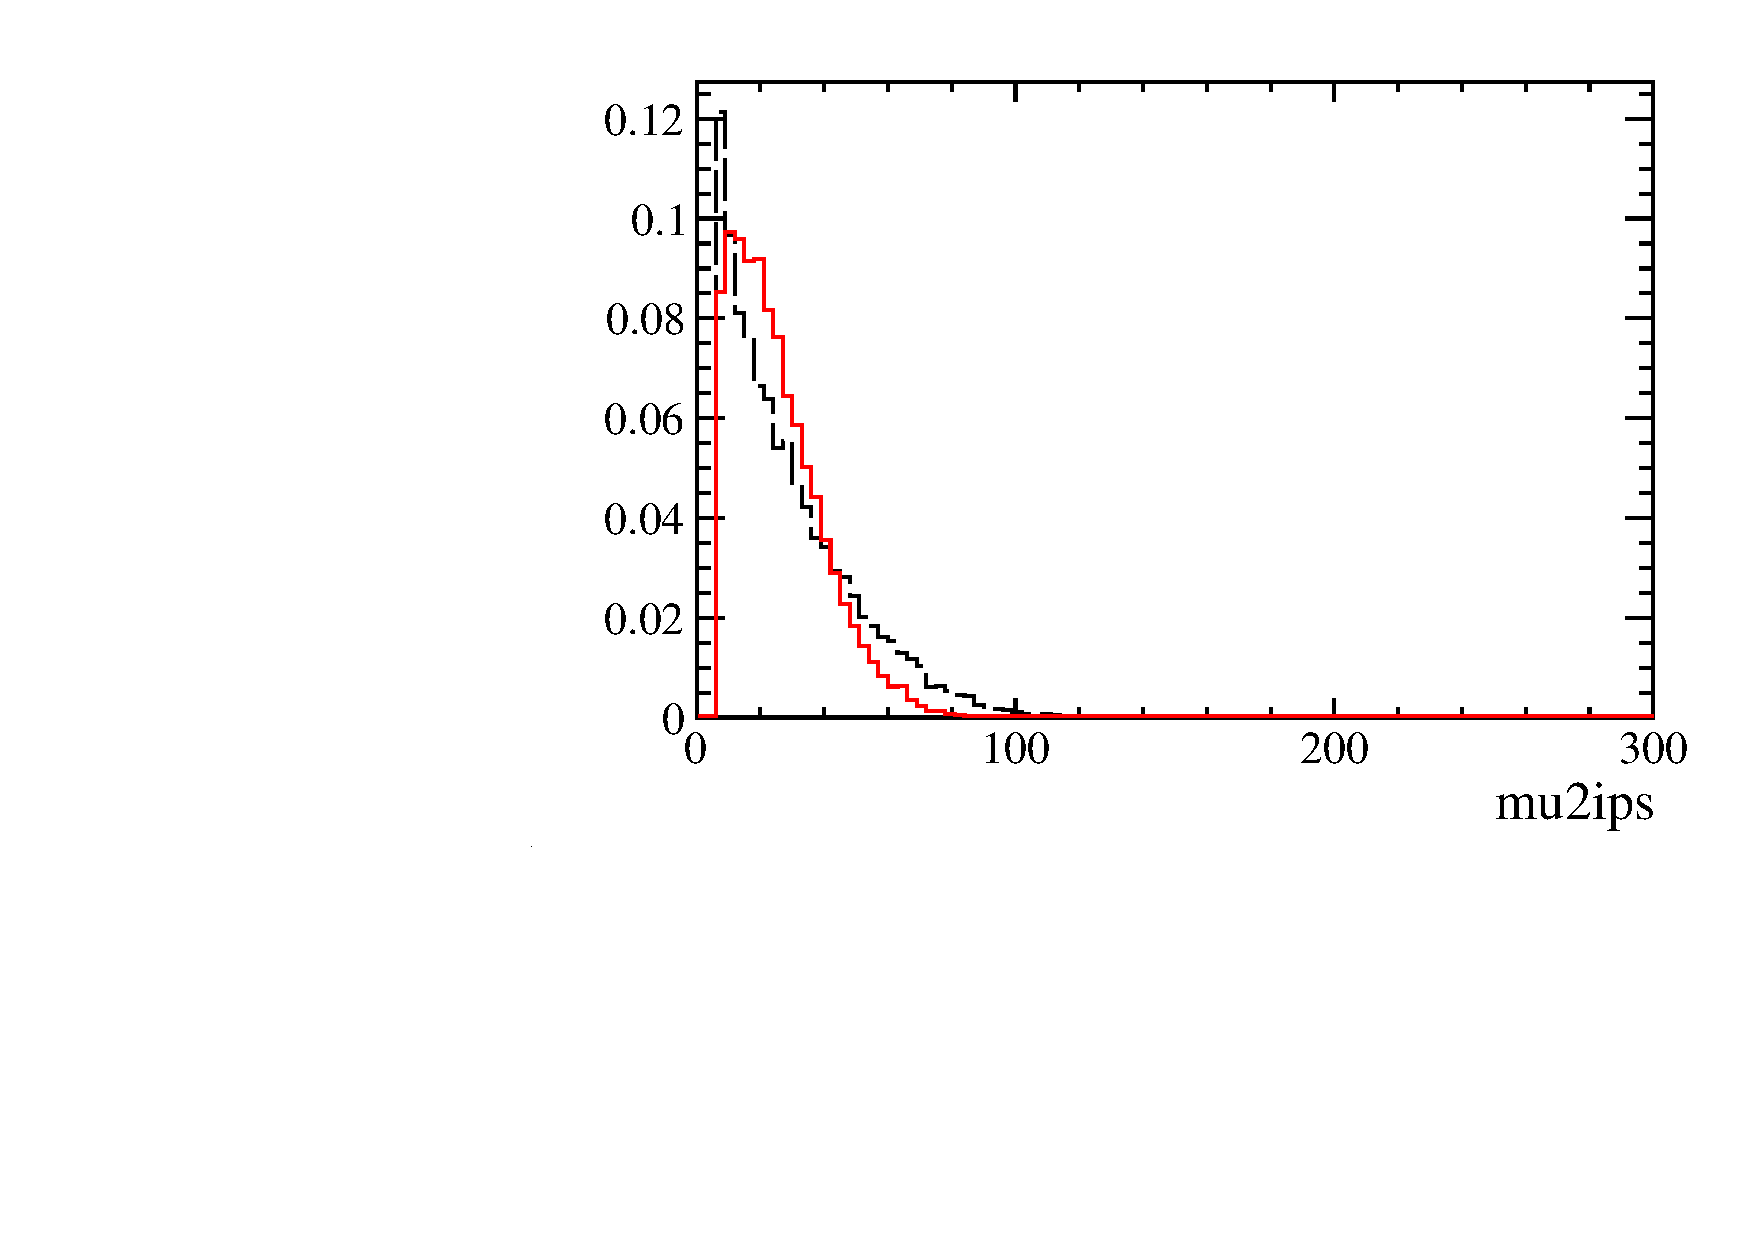
\includegraphics[scale=0.20]{figs/mu2ipsFULL.pdf}
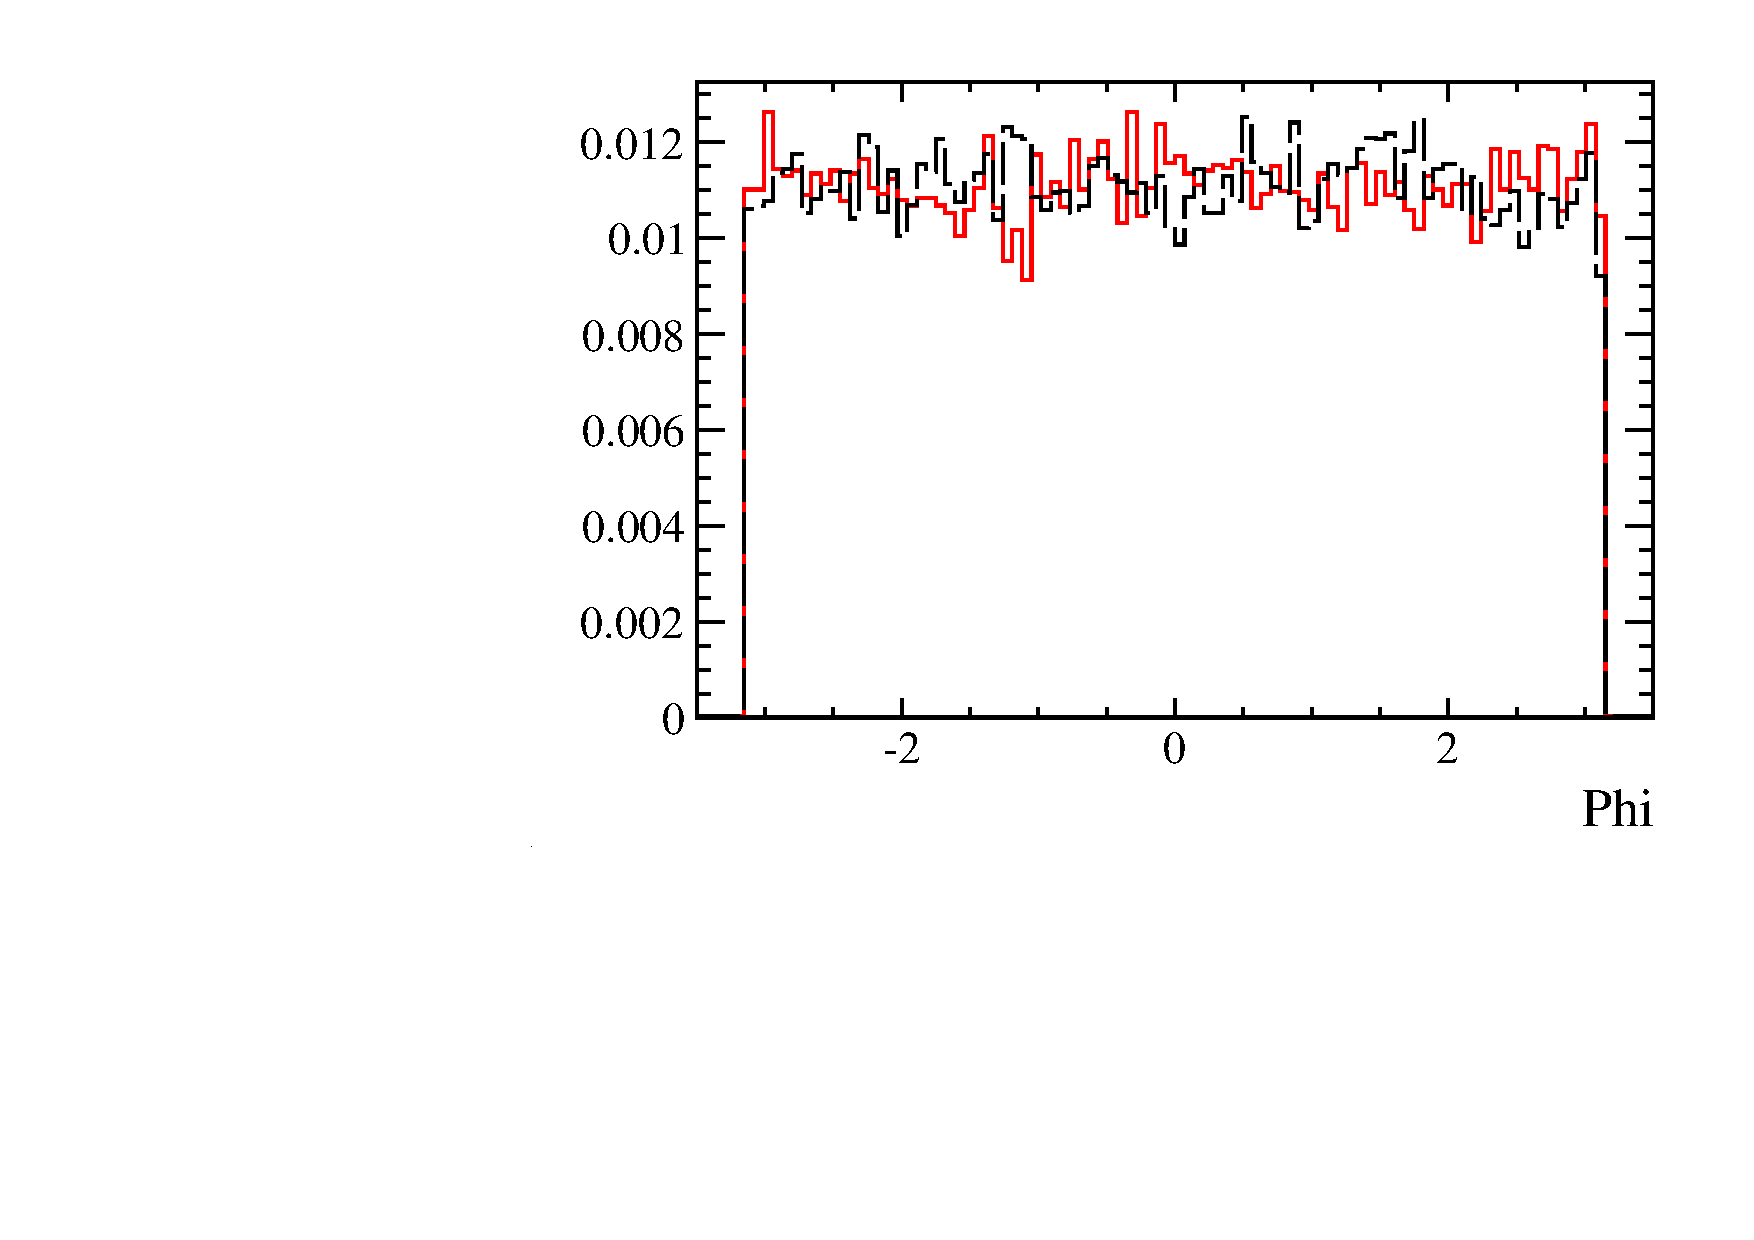
\includegraphics[scale=0.20]{figs/PhiFULL.pdf}
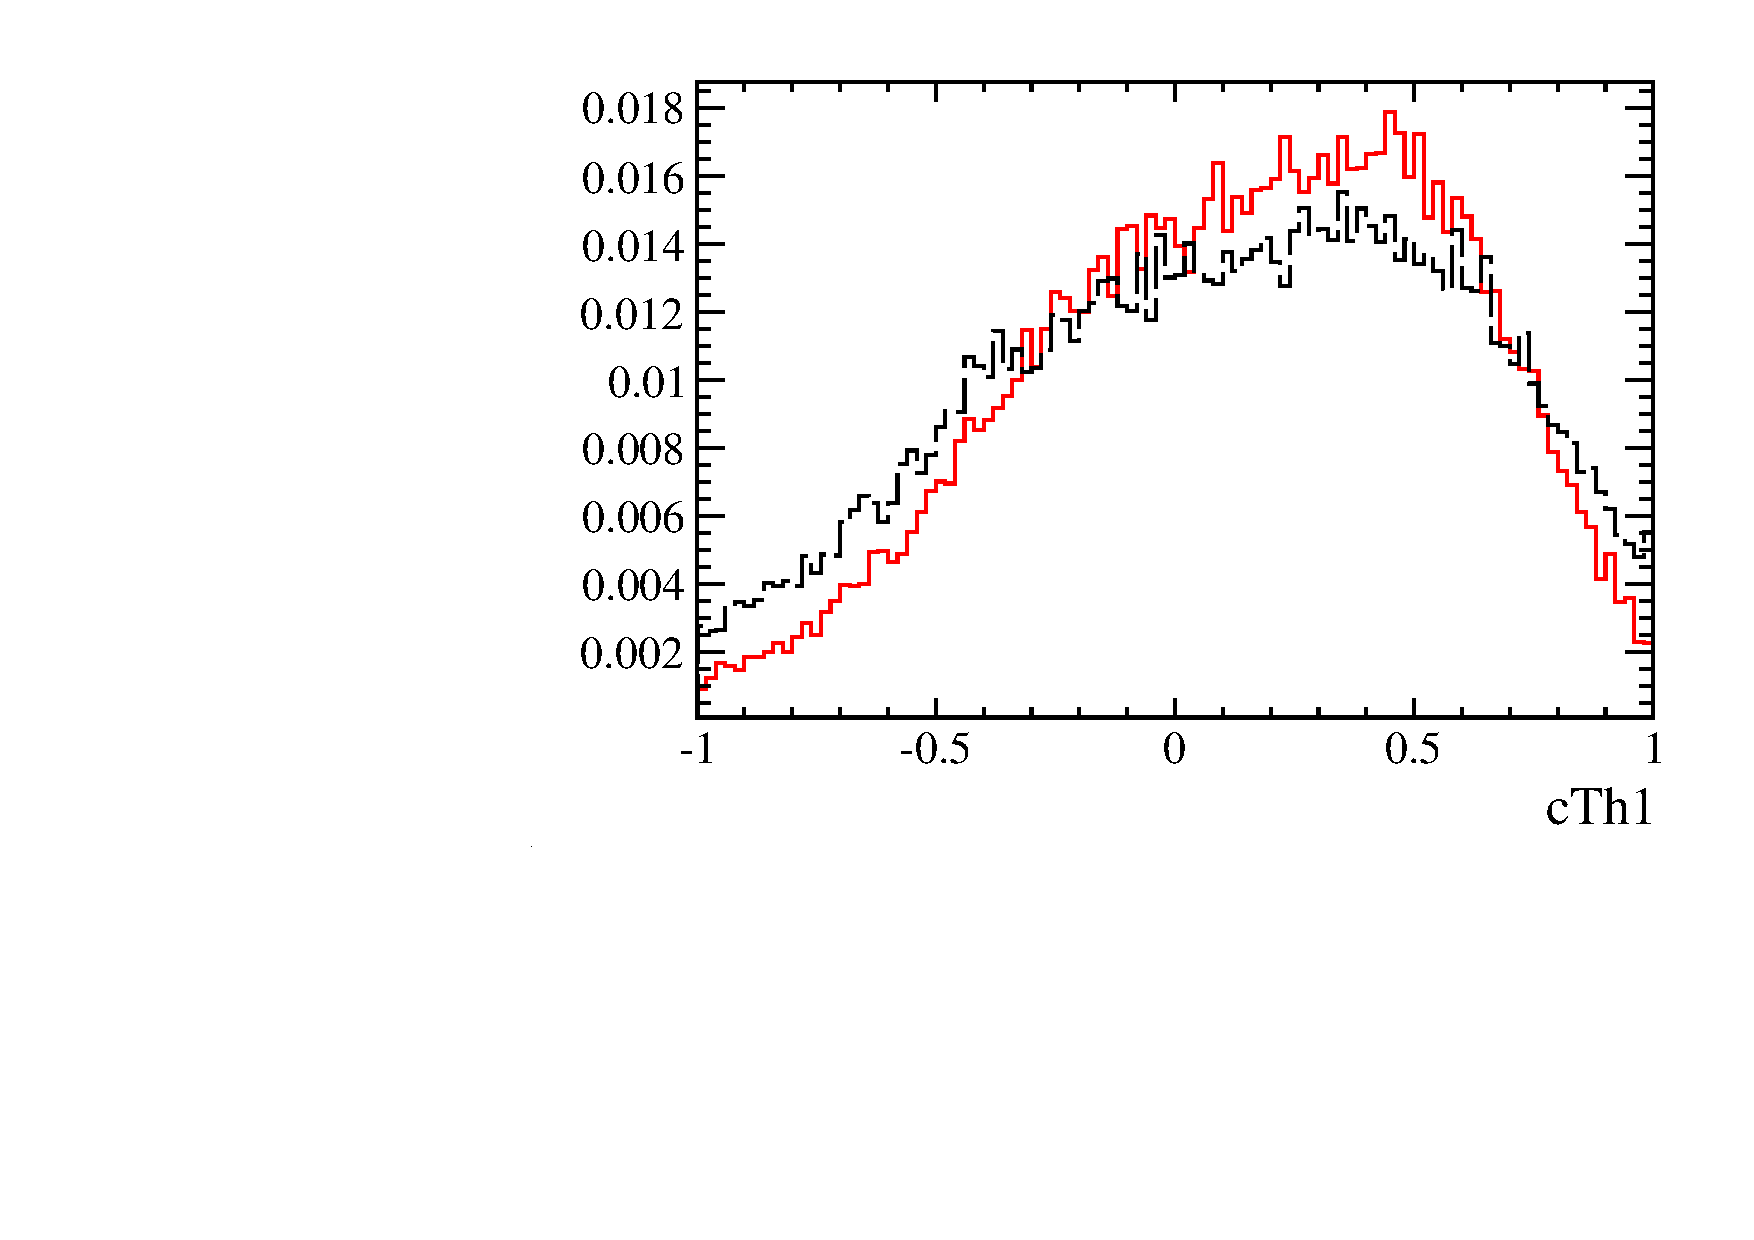
\includegraphics[scale=0.20]{figs/cTh1FULL.pdf}
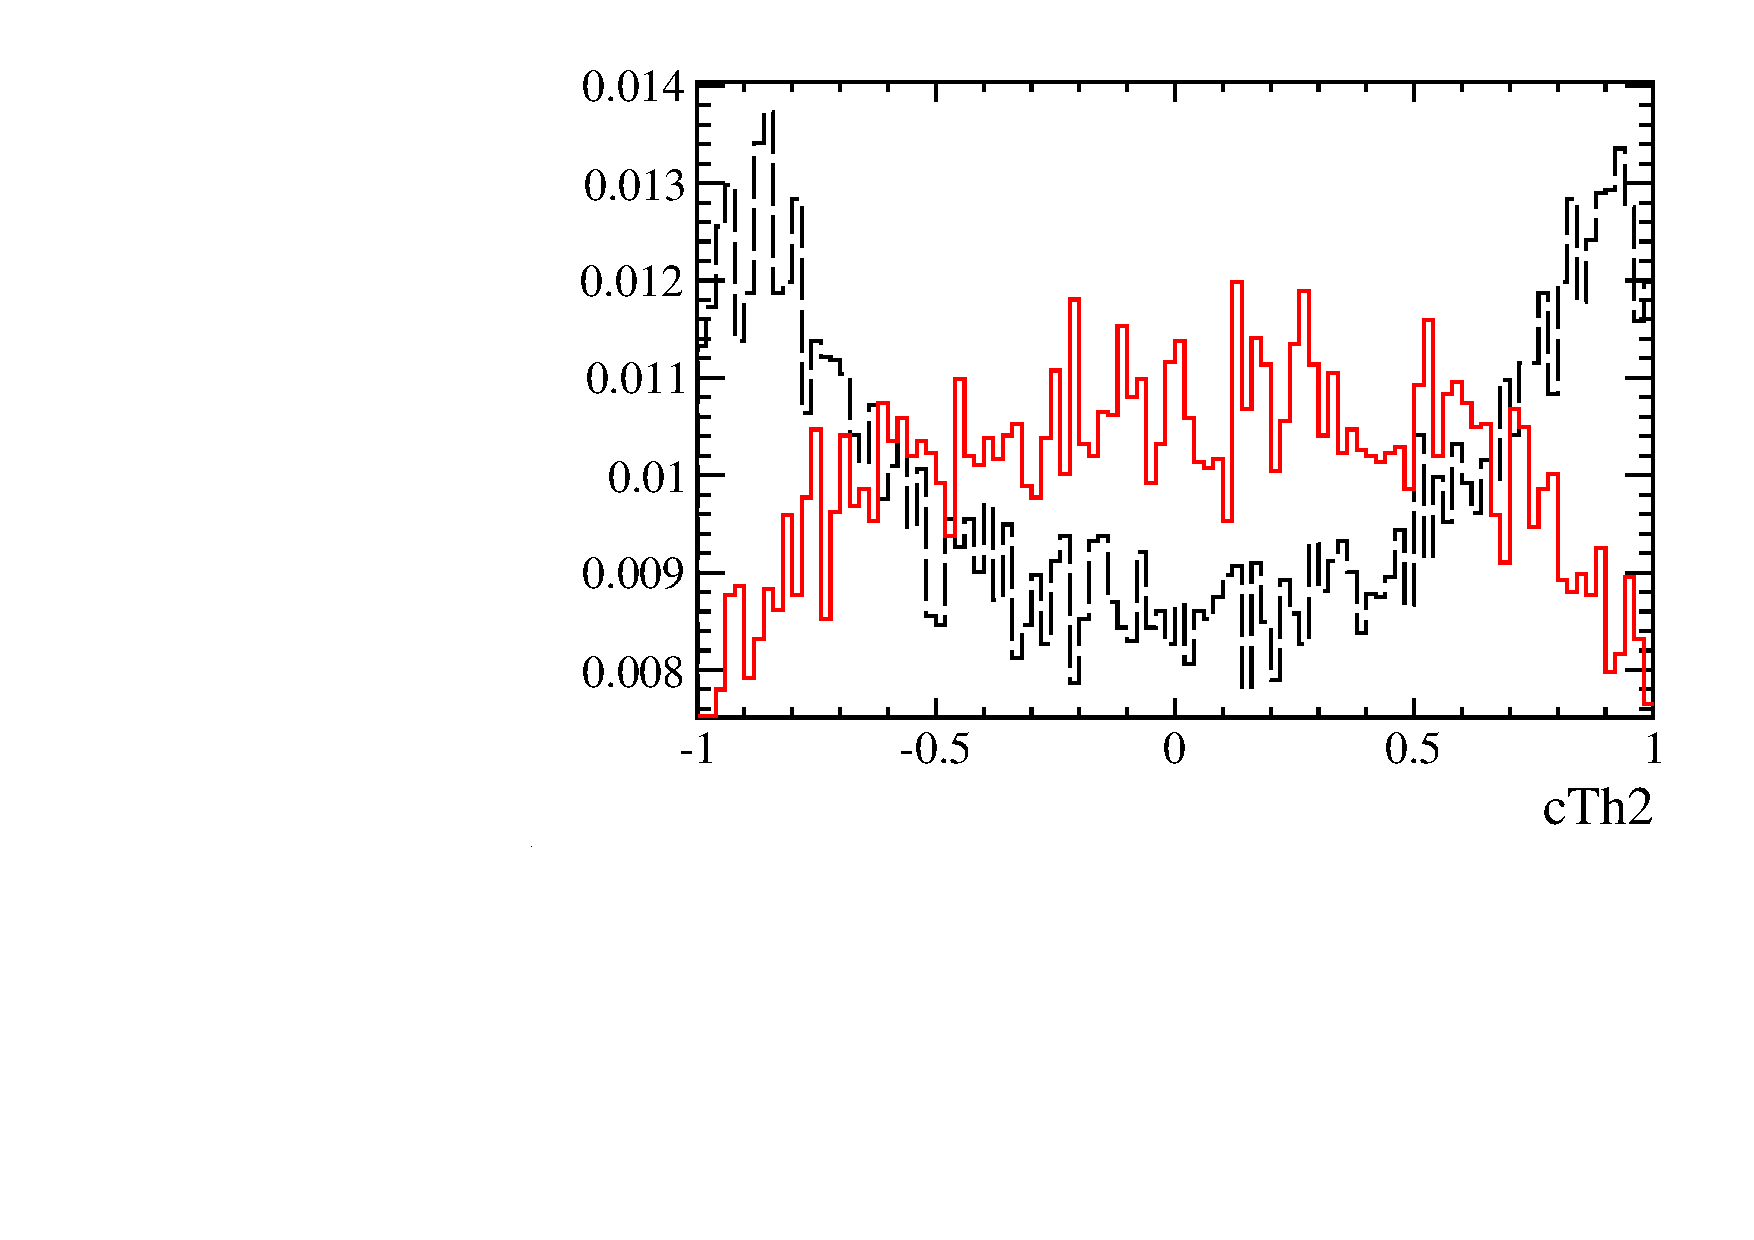
\includegraphics[scale=0.20]{figs/cTh2FULL.pdf}
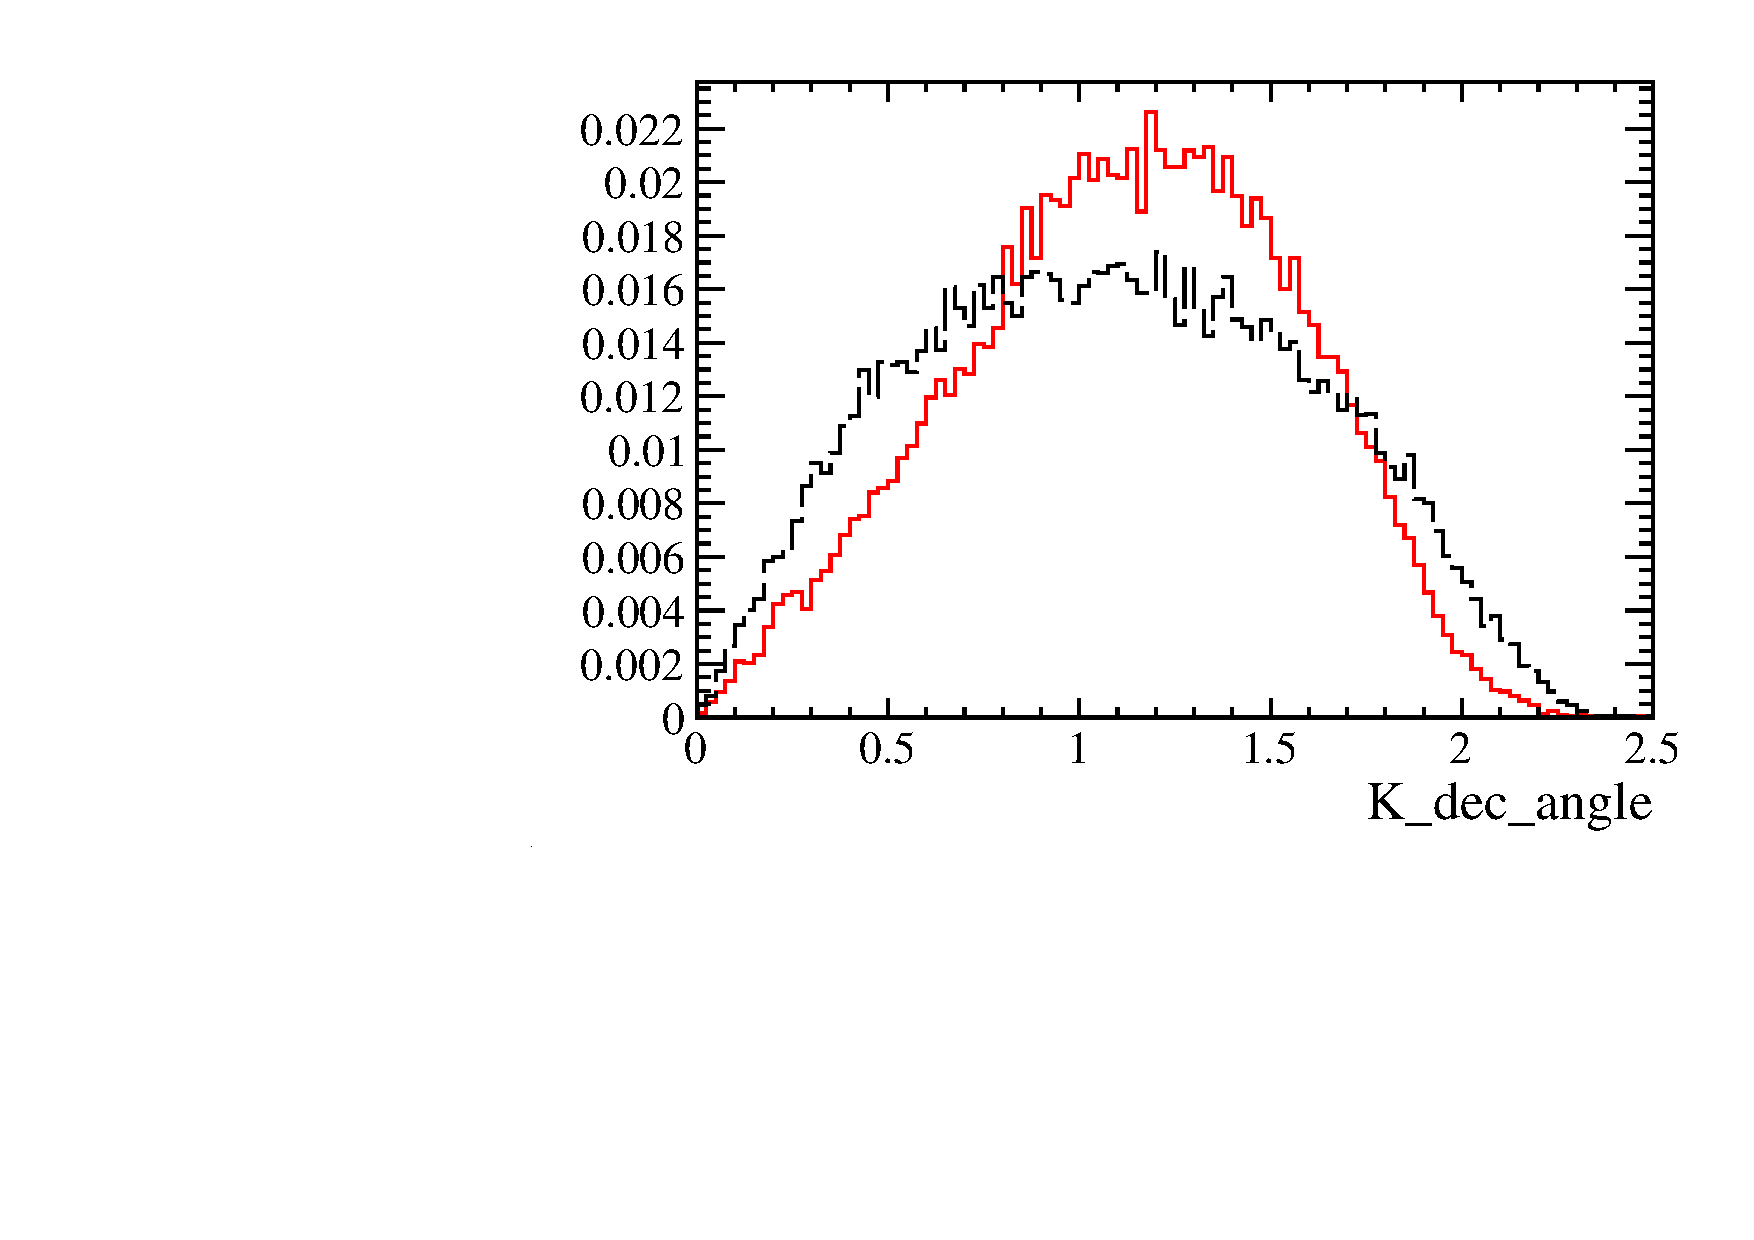
\includegraphics[scale=0.20]{figs/K_dec_angleFULL.pdf}
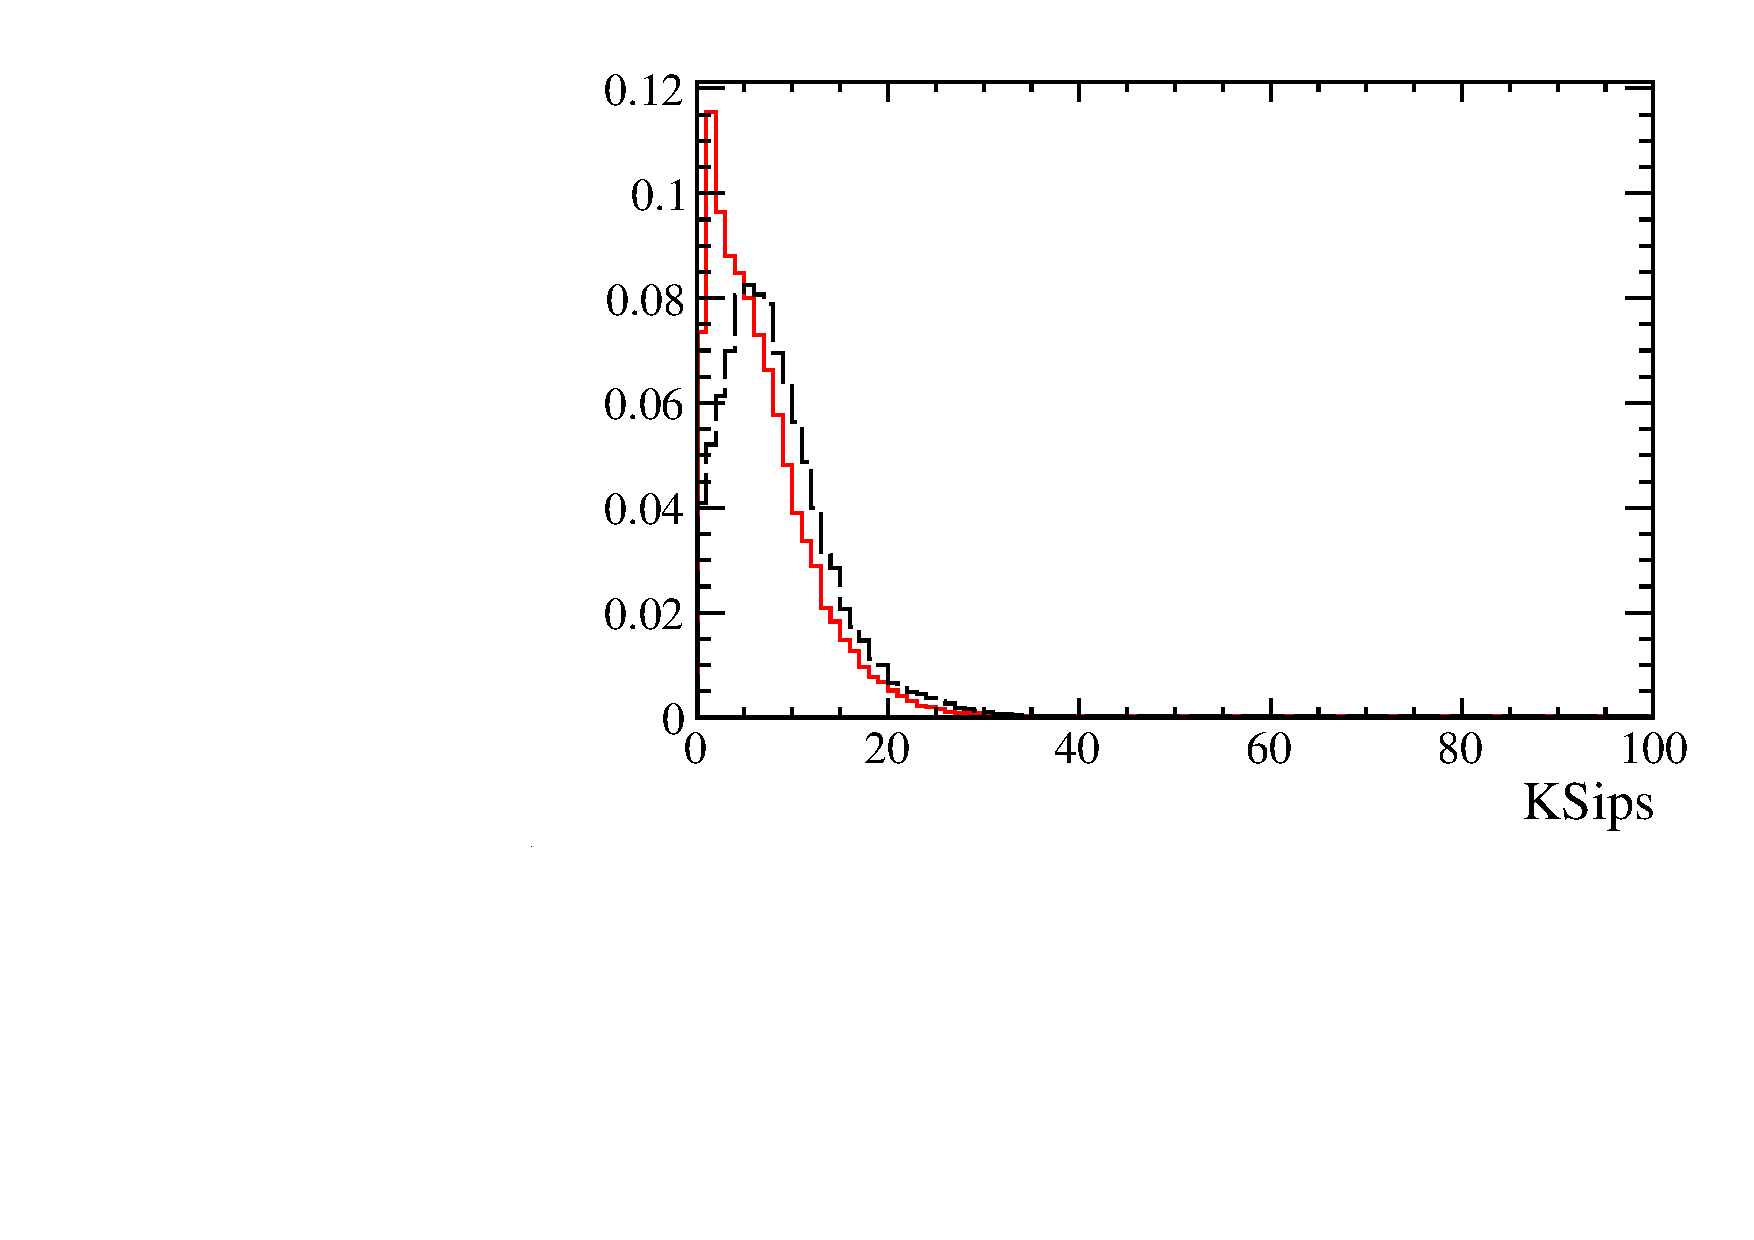
\includegraphics[scale=0.20]{figs/KSipsFULL.pdf}
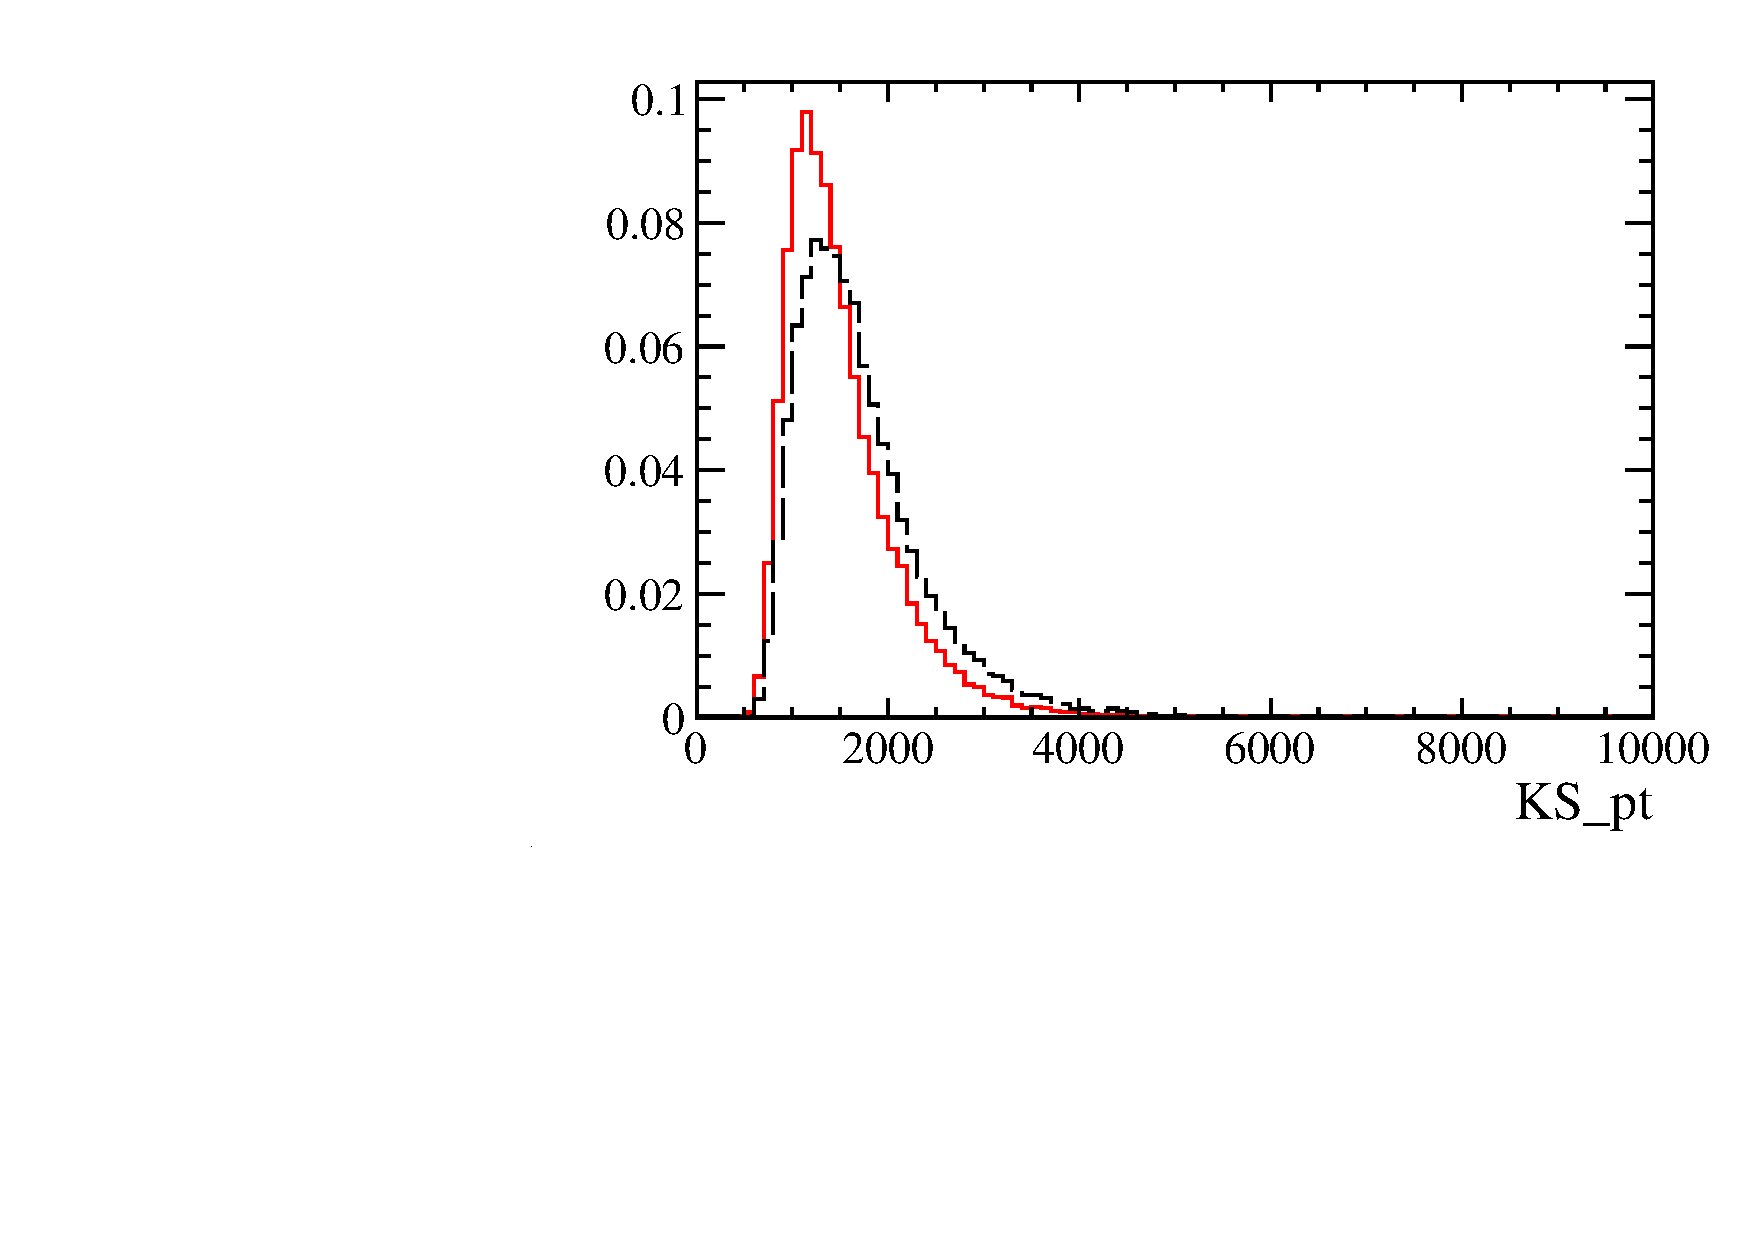
\includegraphics[scale=0.20]{figs/KS_ptFULL.pdf}
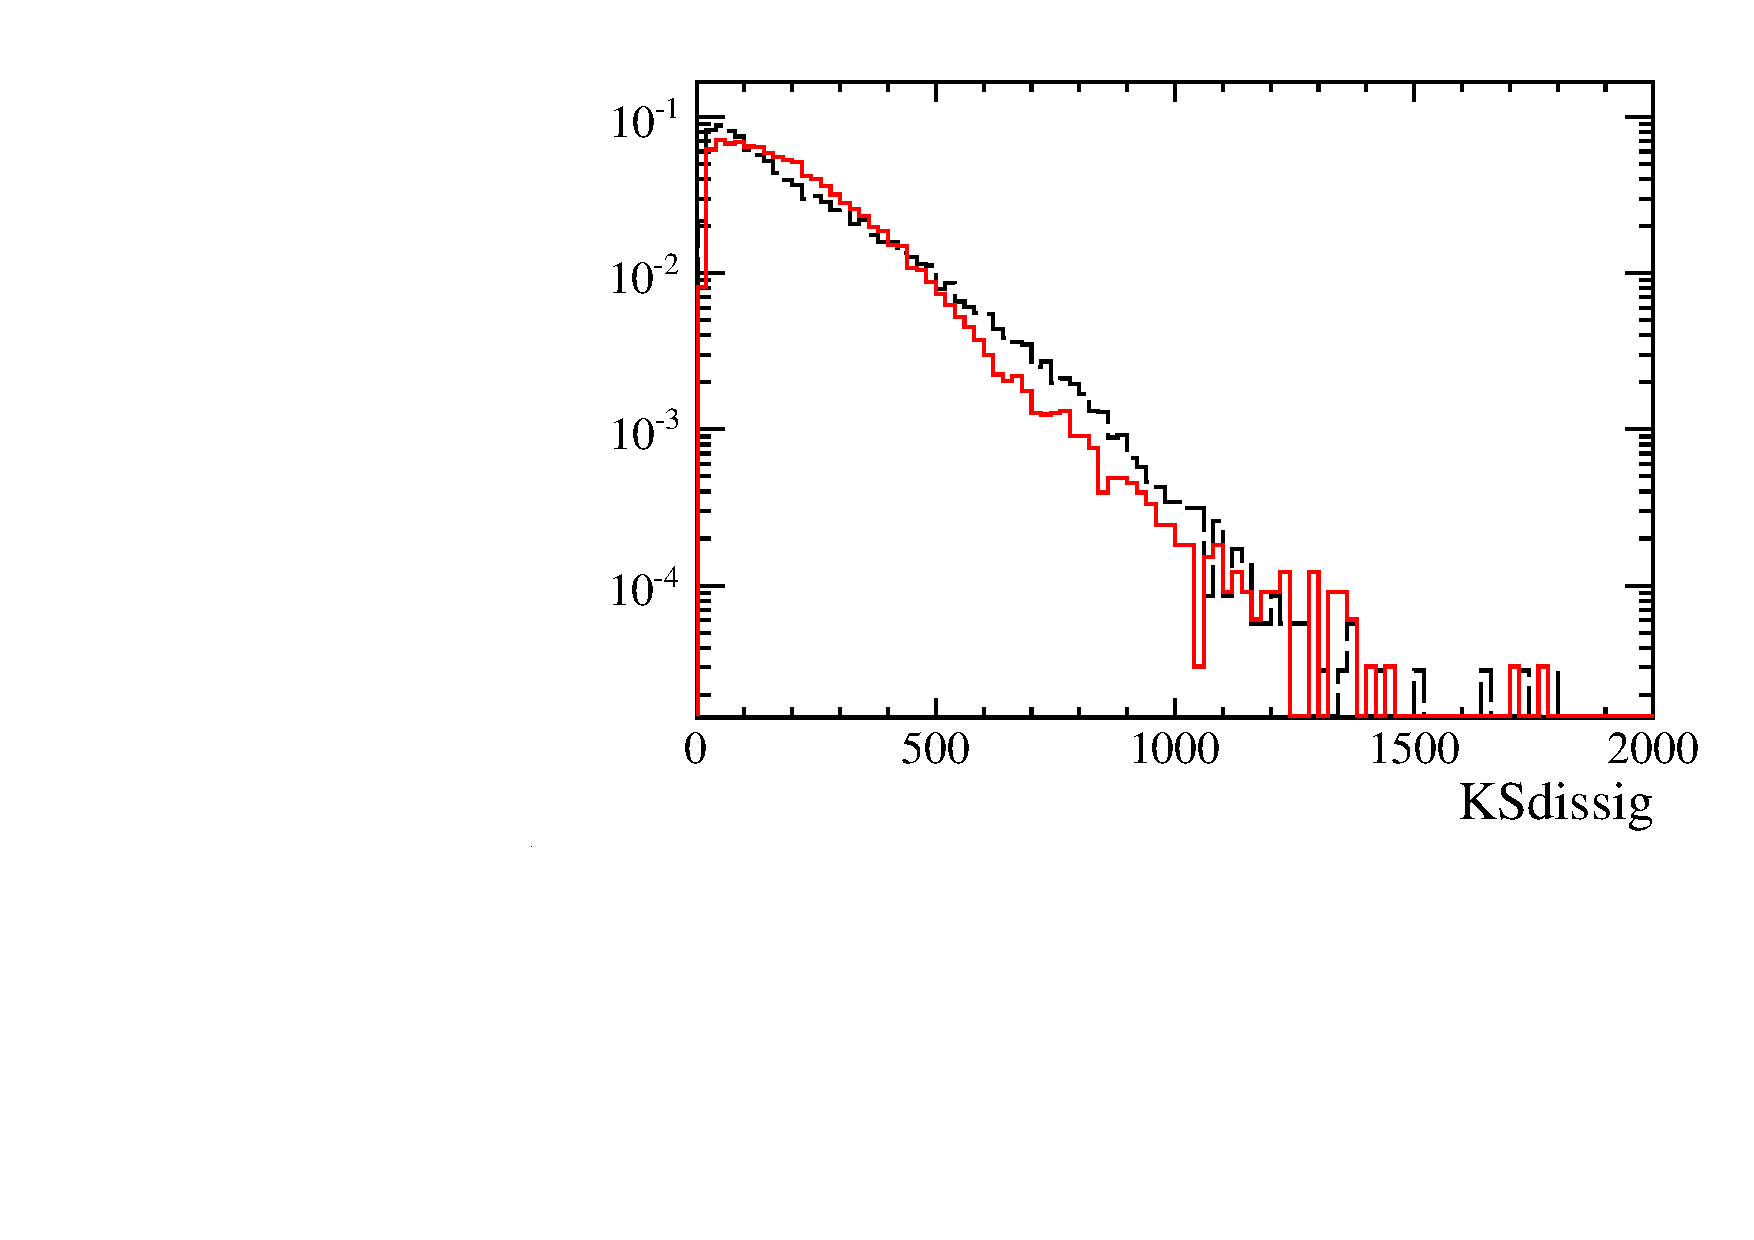
\includegraphics[scale=0.20]{figs/KSdissigFULL.pdf}
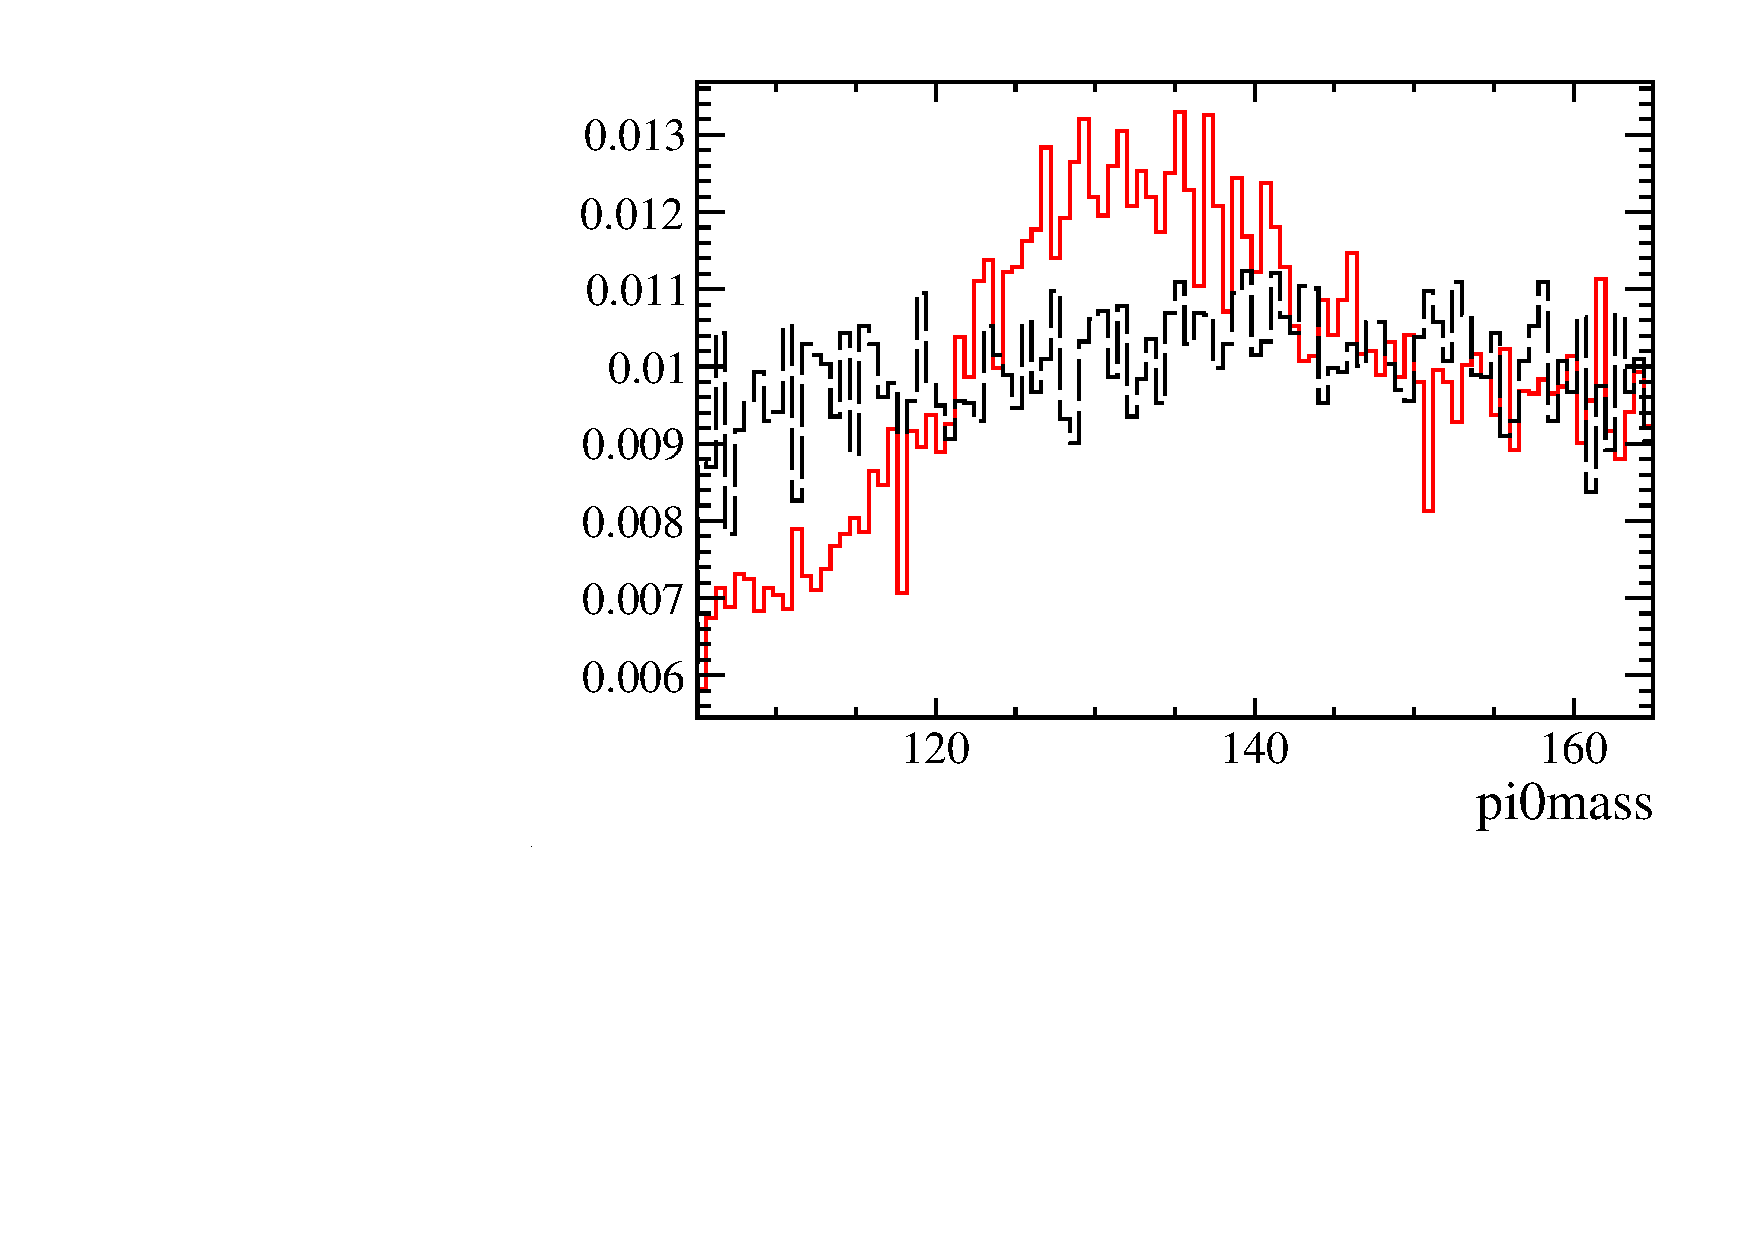
\includegraphics[scale=0.20]{figs/pi0massFULL.pdf}
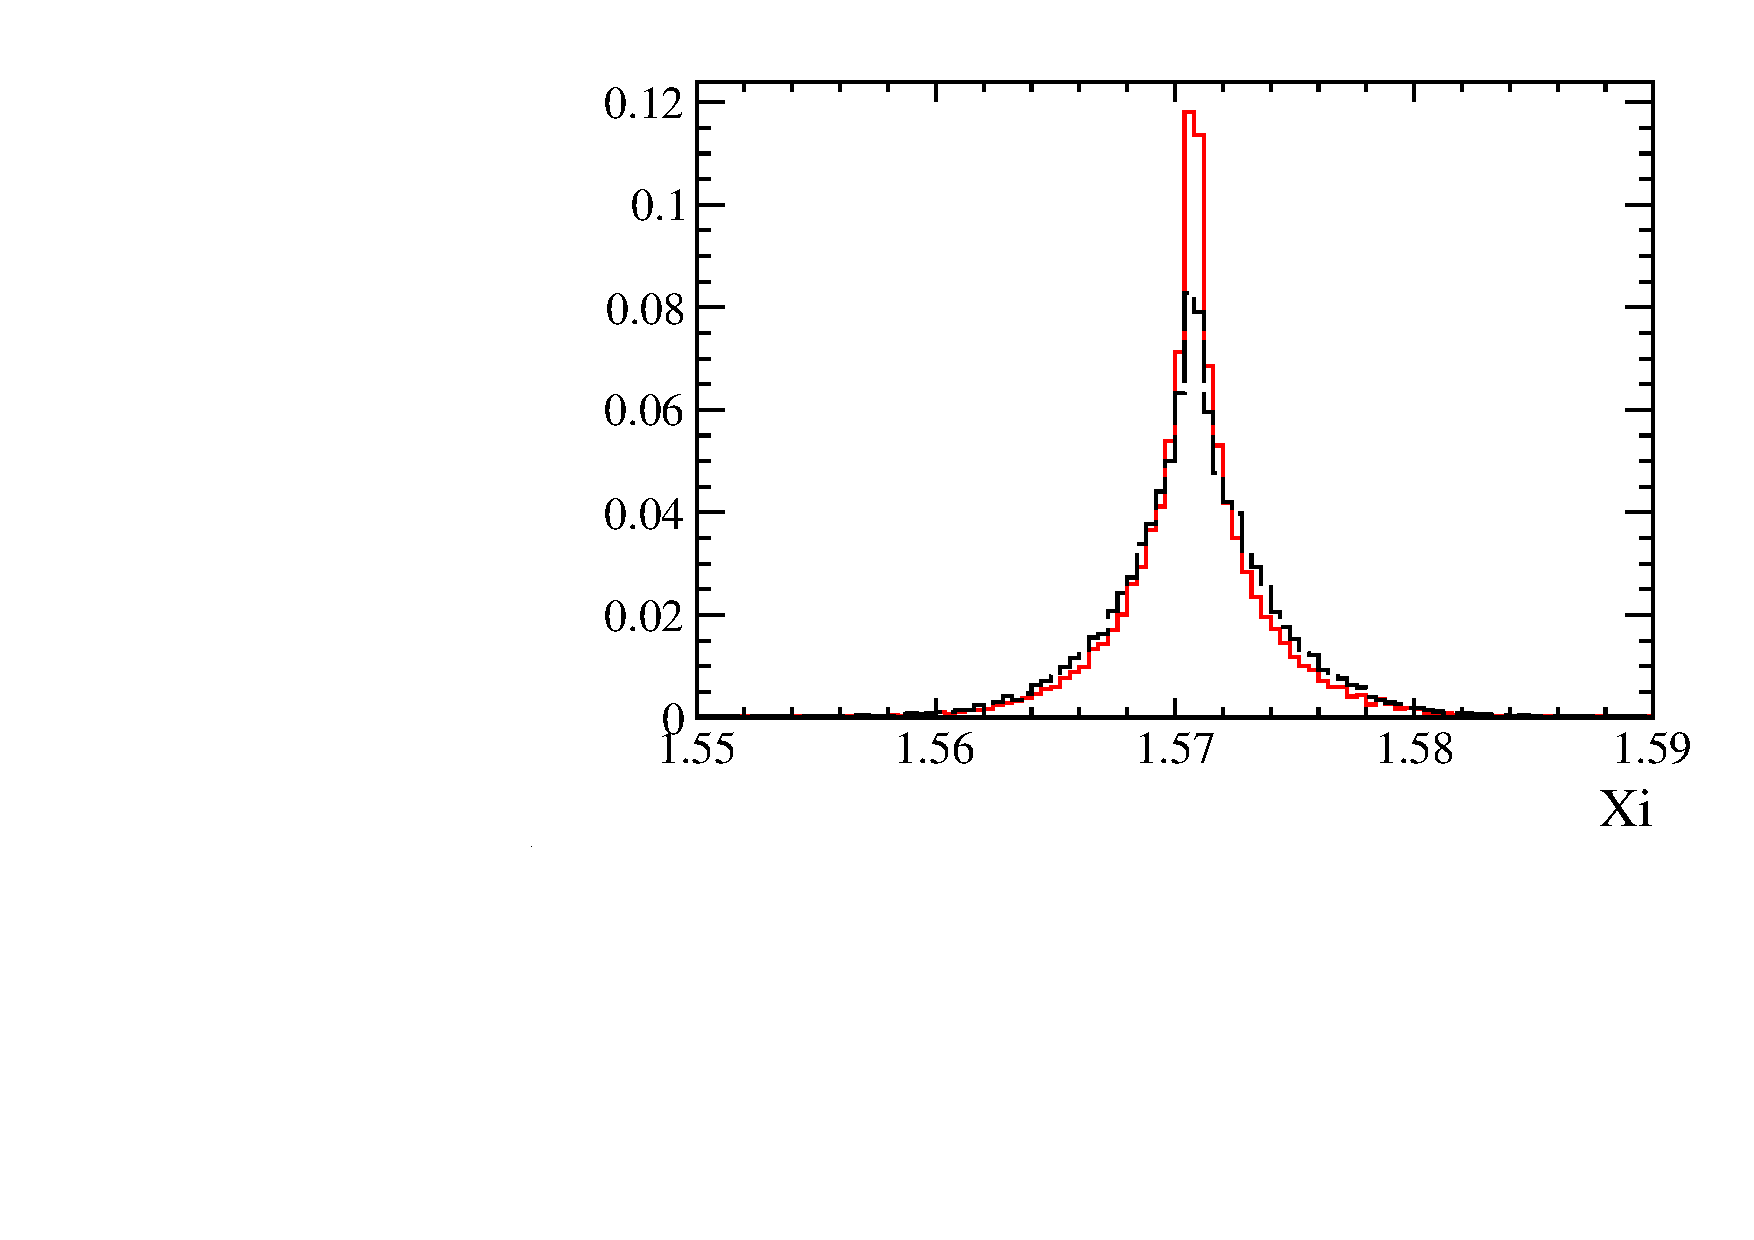
\includegraphics[scale=0.20]{figs/XiFULL.pdf}
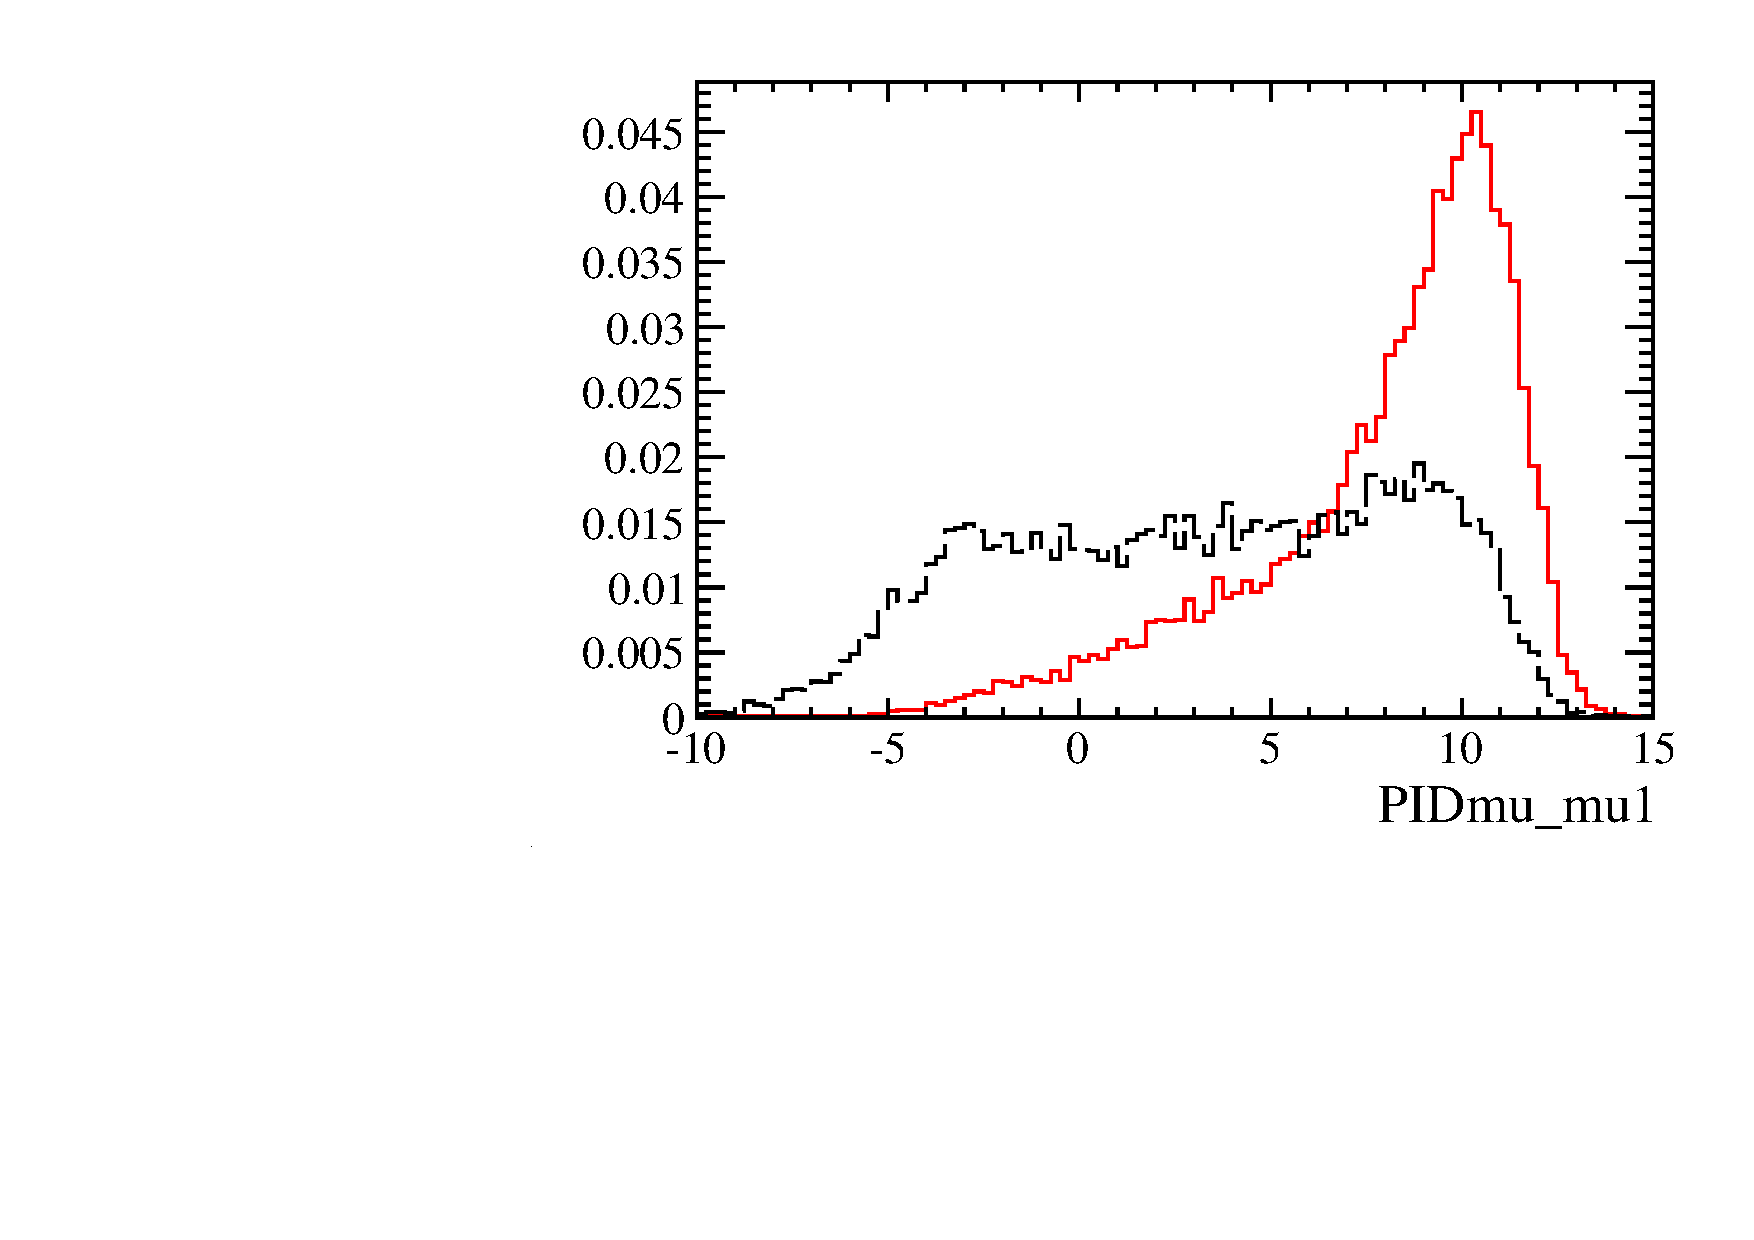
\includegraphics[scale=0.20]{figs/PIDmu_mu1FULL.pdf}
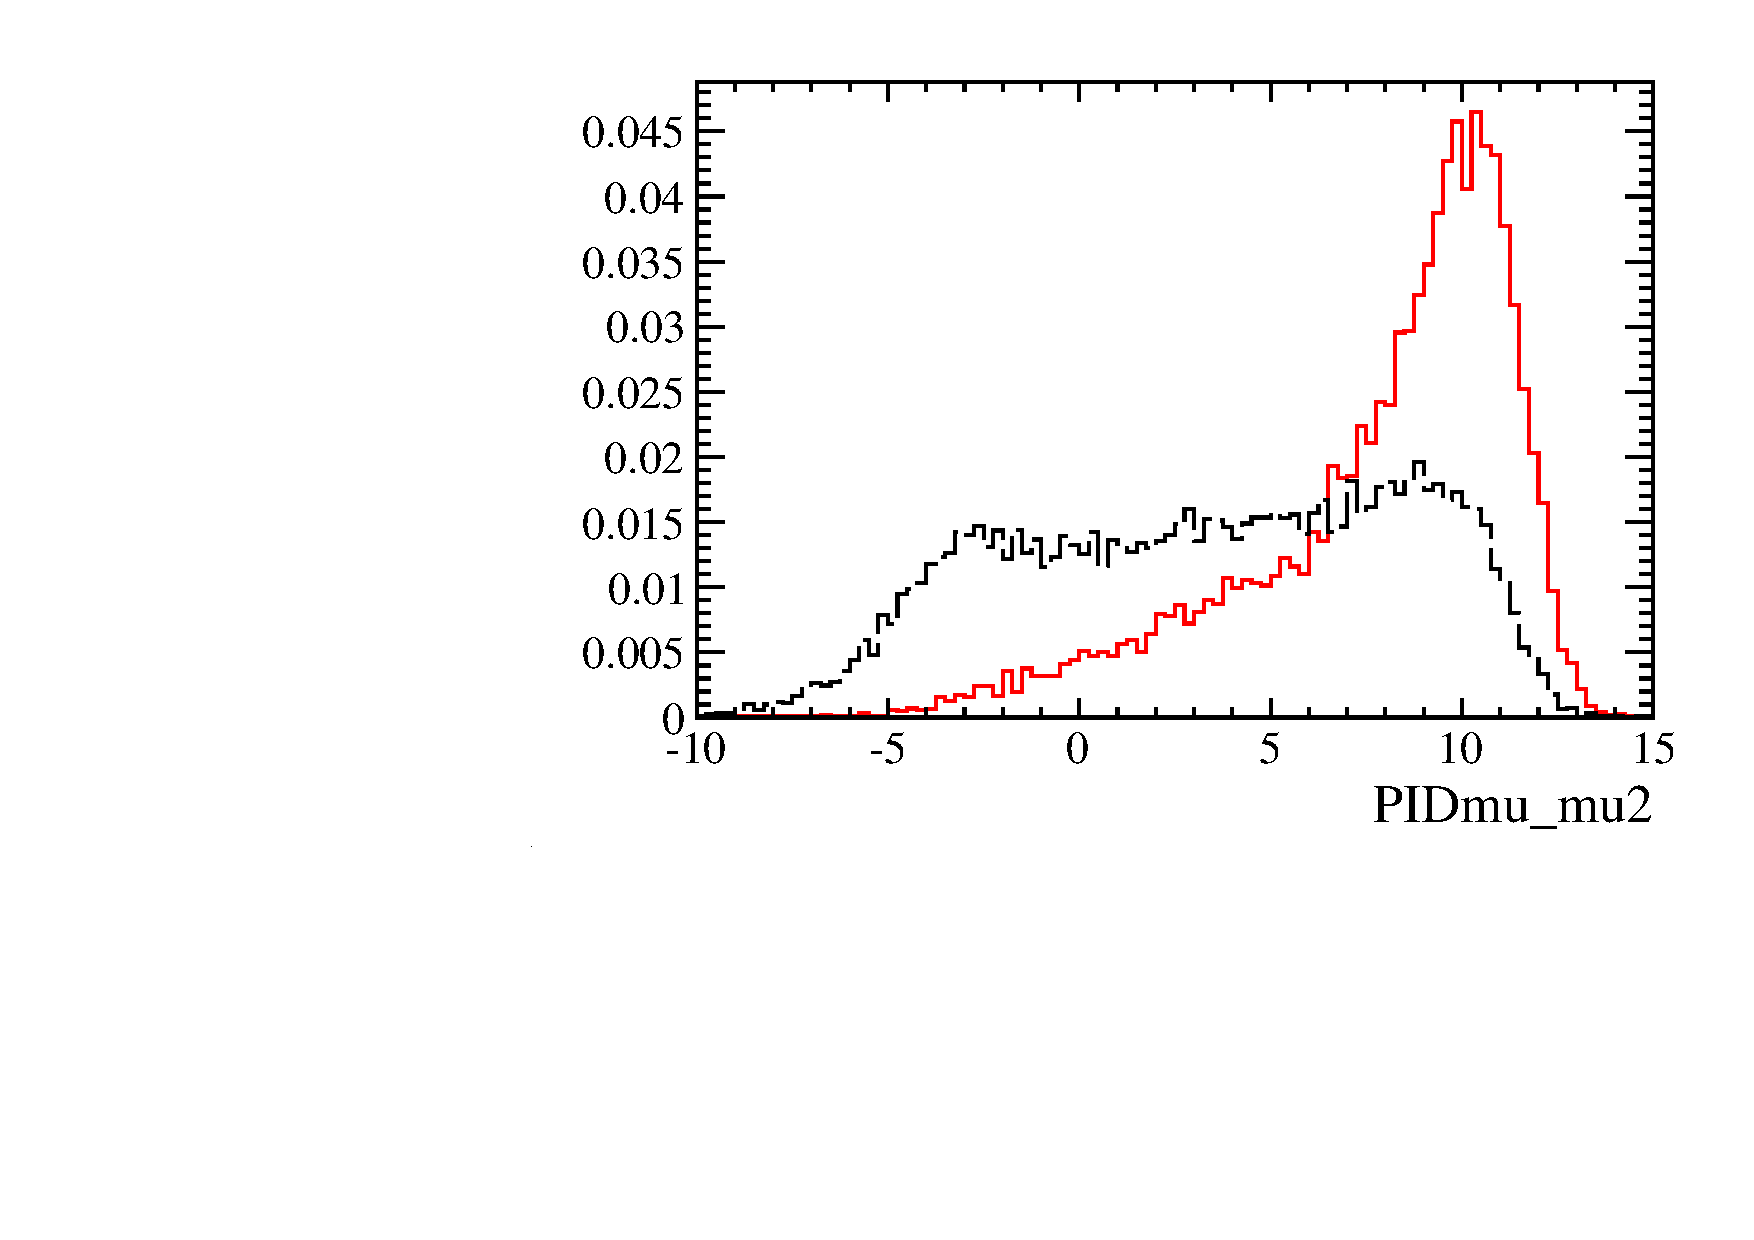
\includegraphics[scale=0.20]{figs/PIDmu_mu2FULL.pdf}
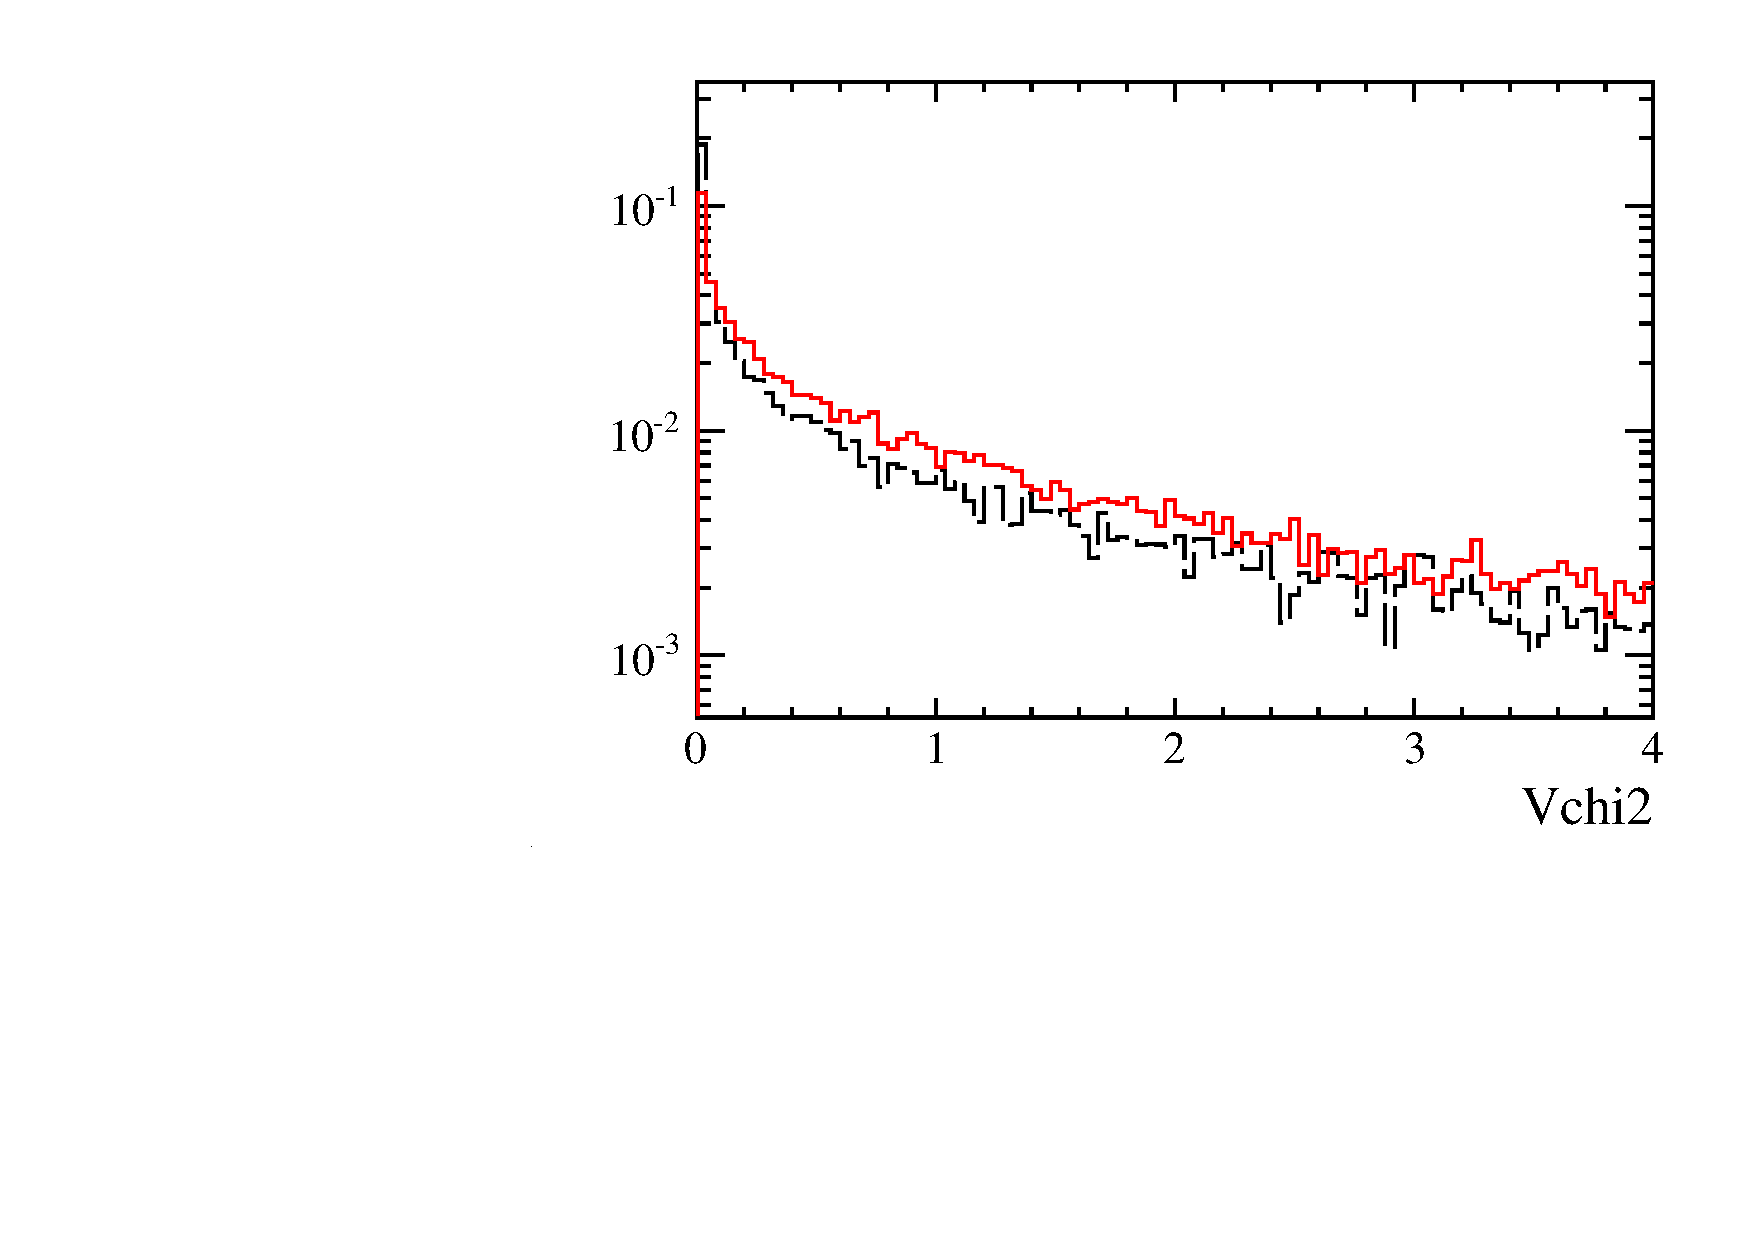
\includegraphics[scale=0.20]{figs/Vchi2FULL.pdf}
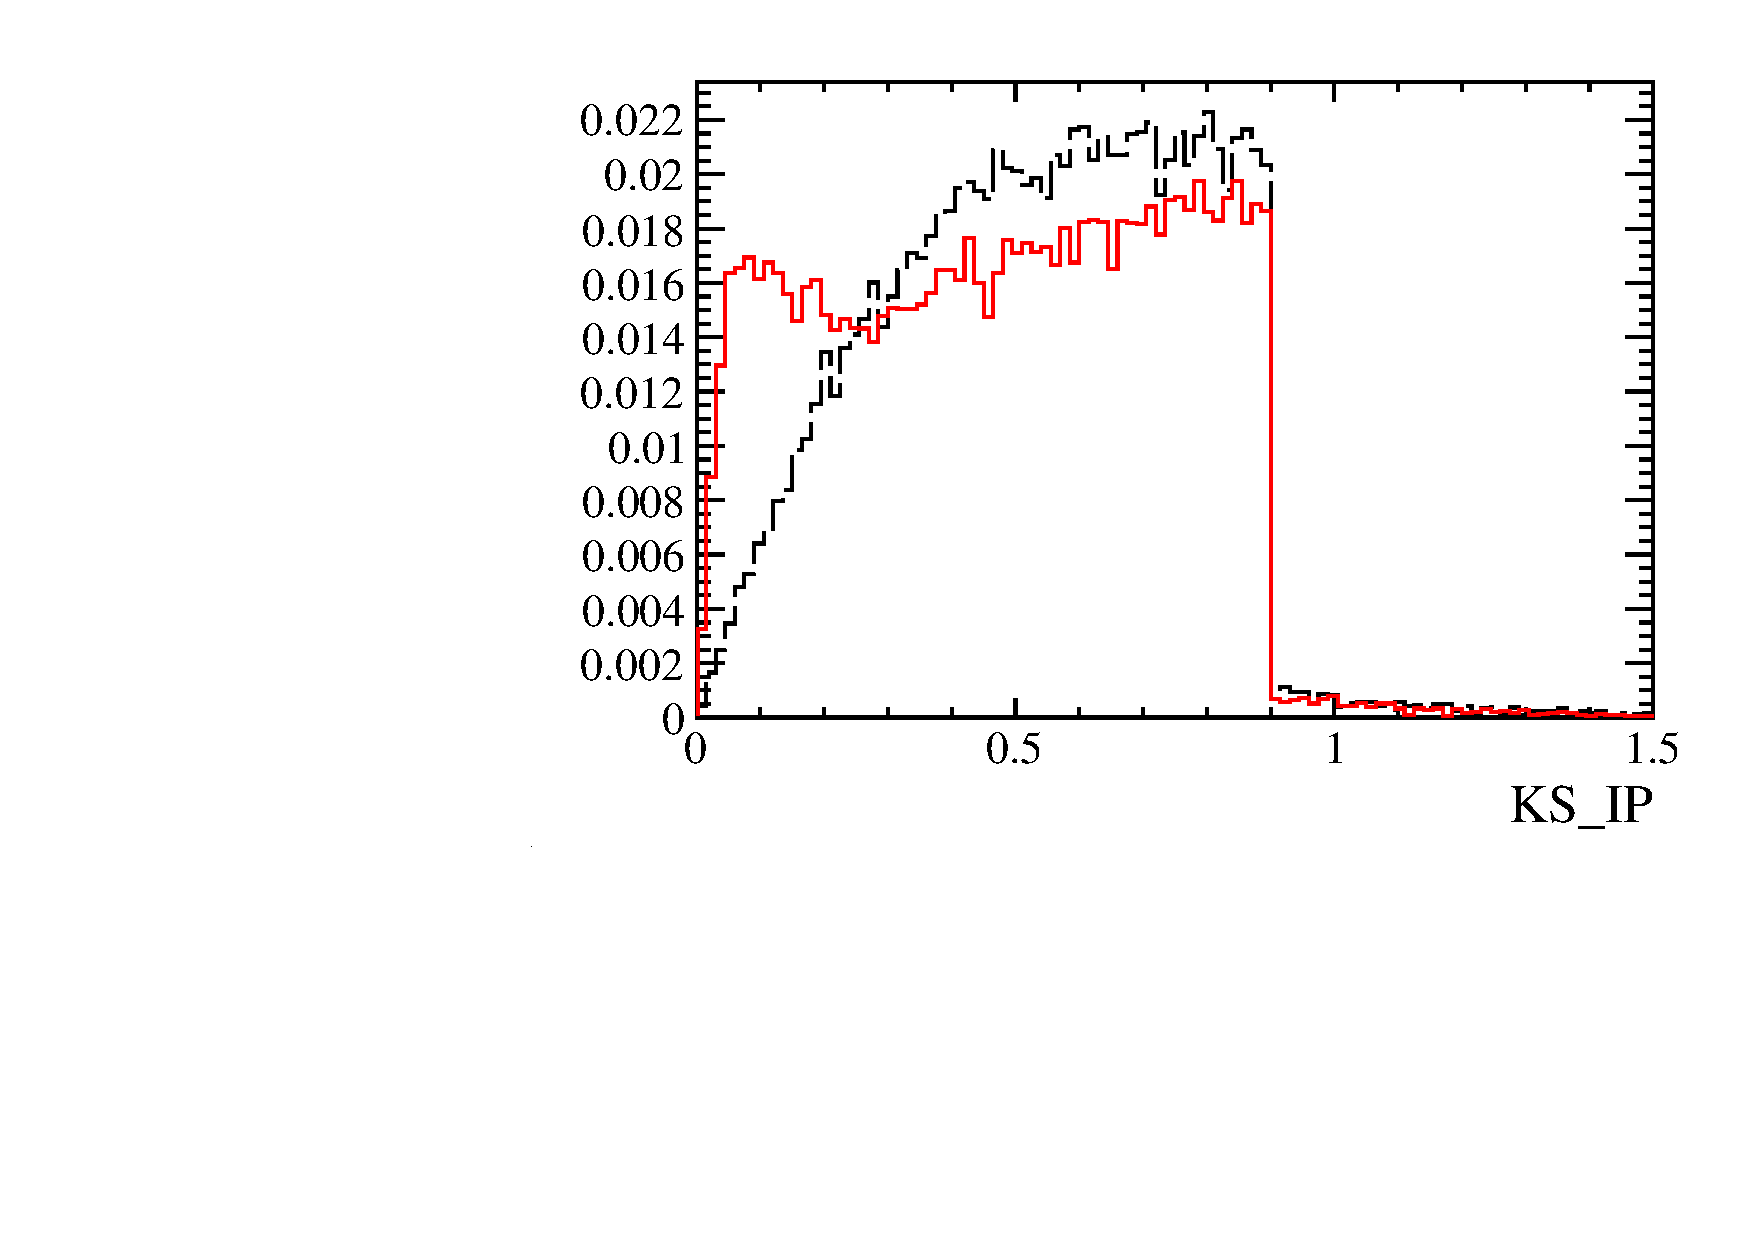
\includegraphics[scale=0.20]{figs/KS_IPFULL.pdf}
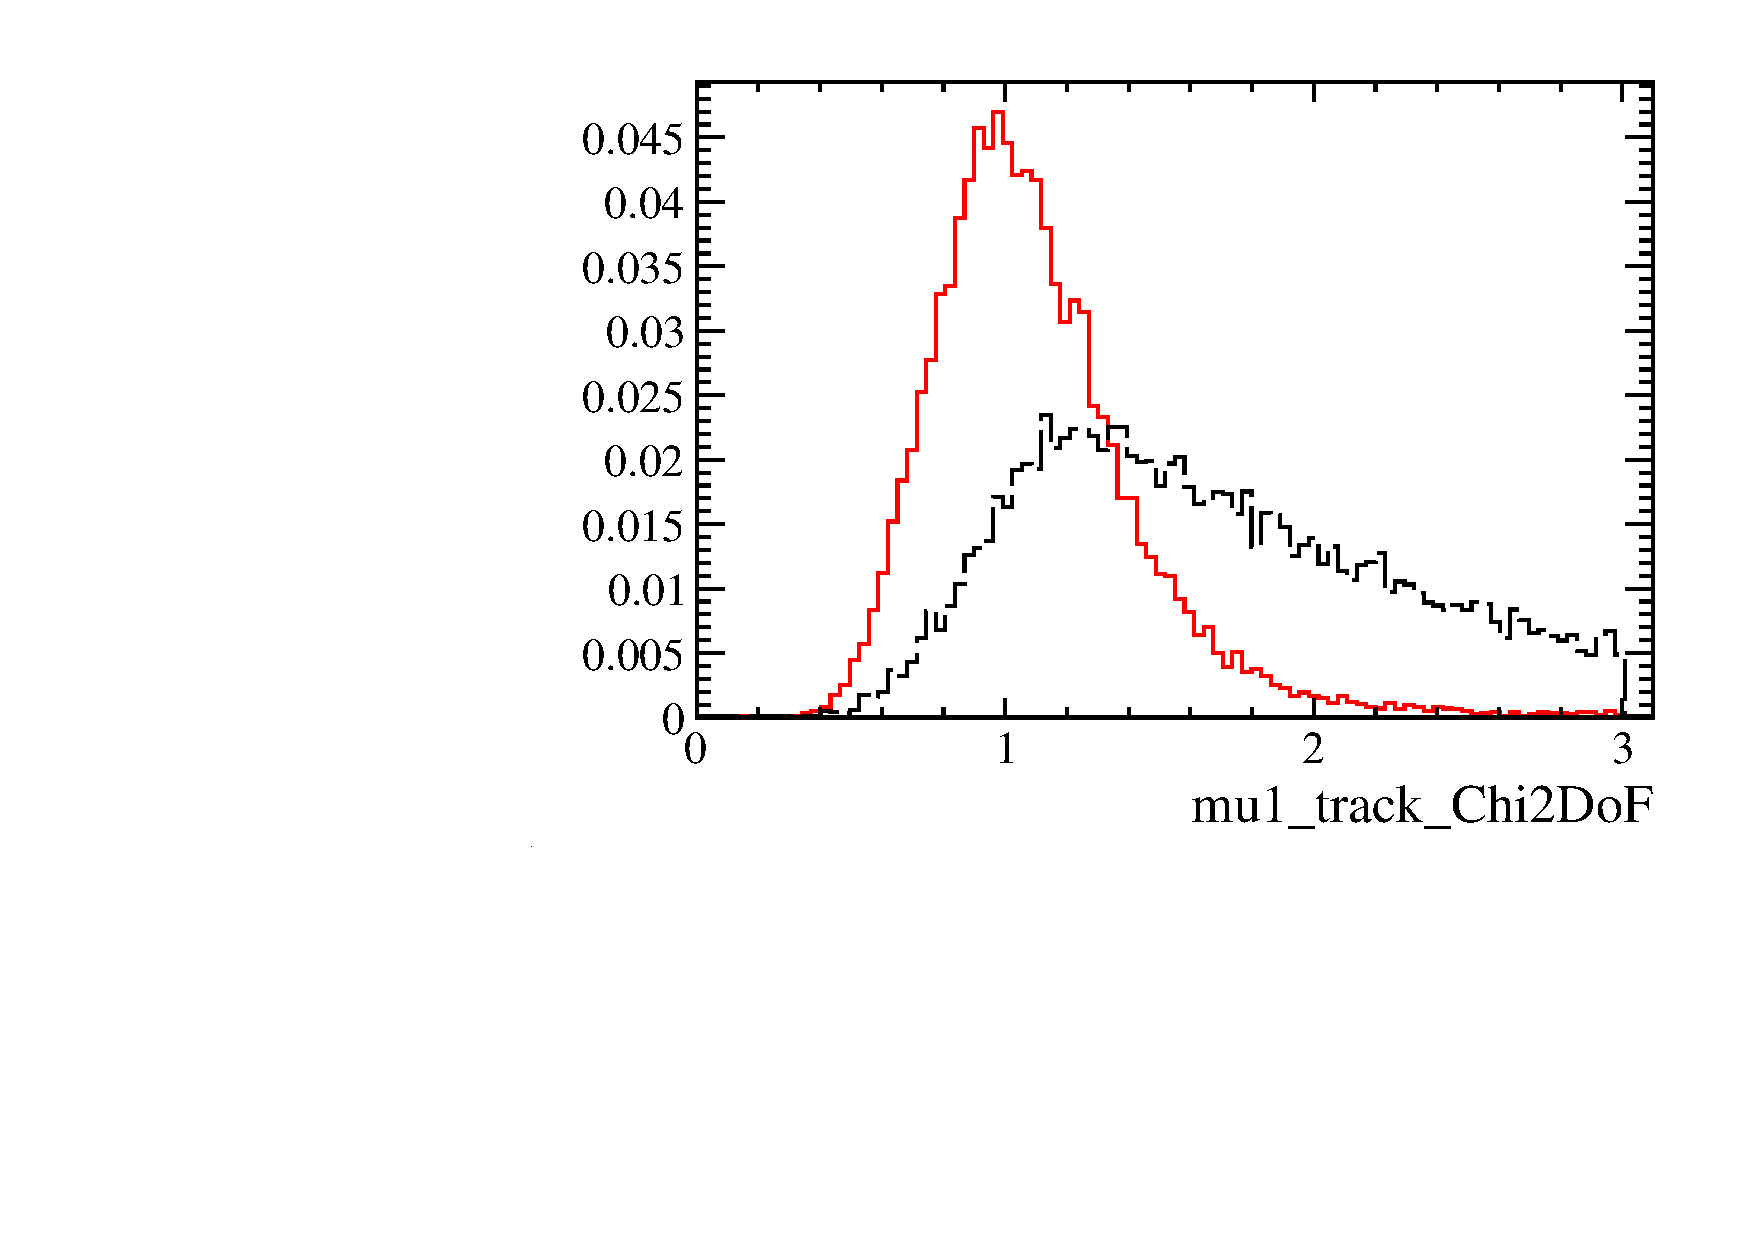
\includegraphics[scale=0.20]{figs/mu1_track_Chi2DoFFULL.pdf}
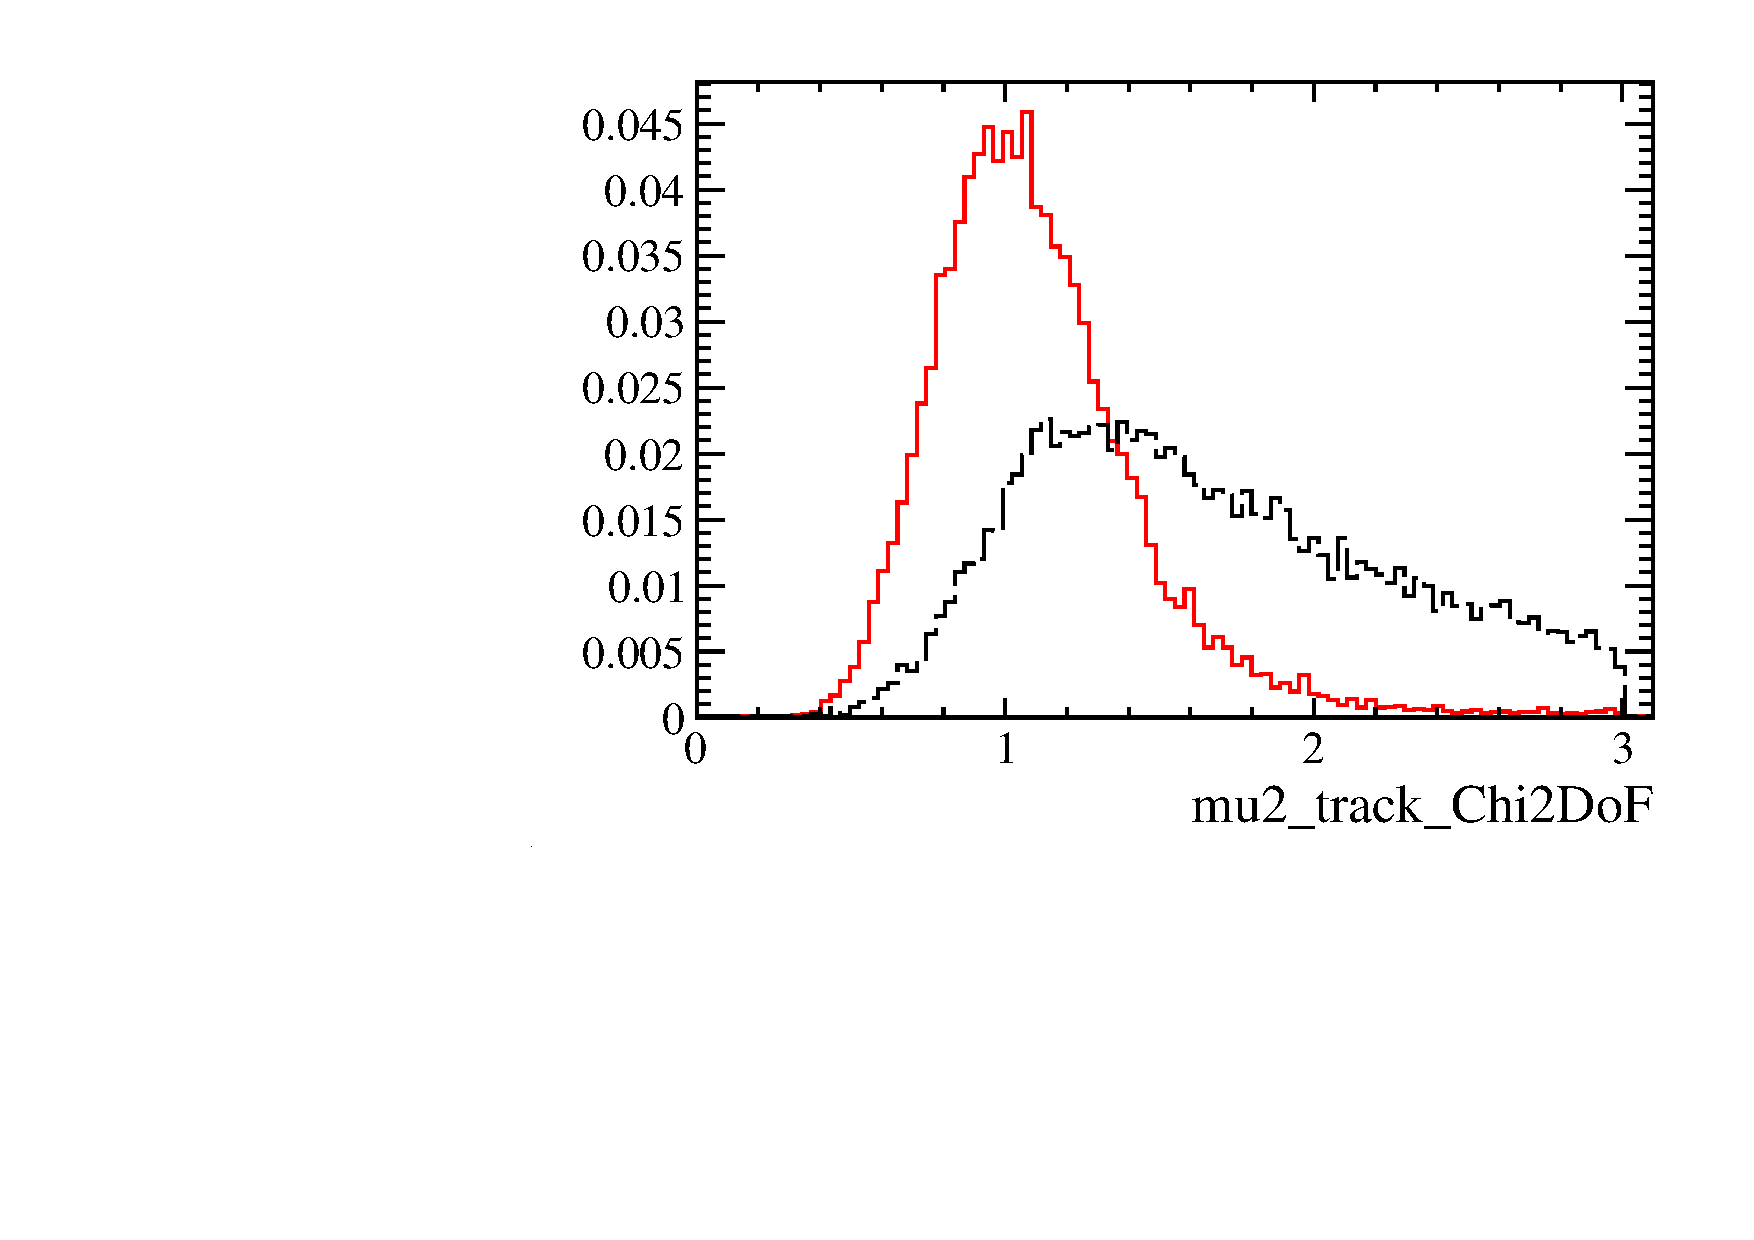
\includegraphics[scale=0.20]{figs/mu2_track_Chi2DoFFULL.pdf}
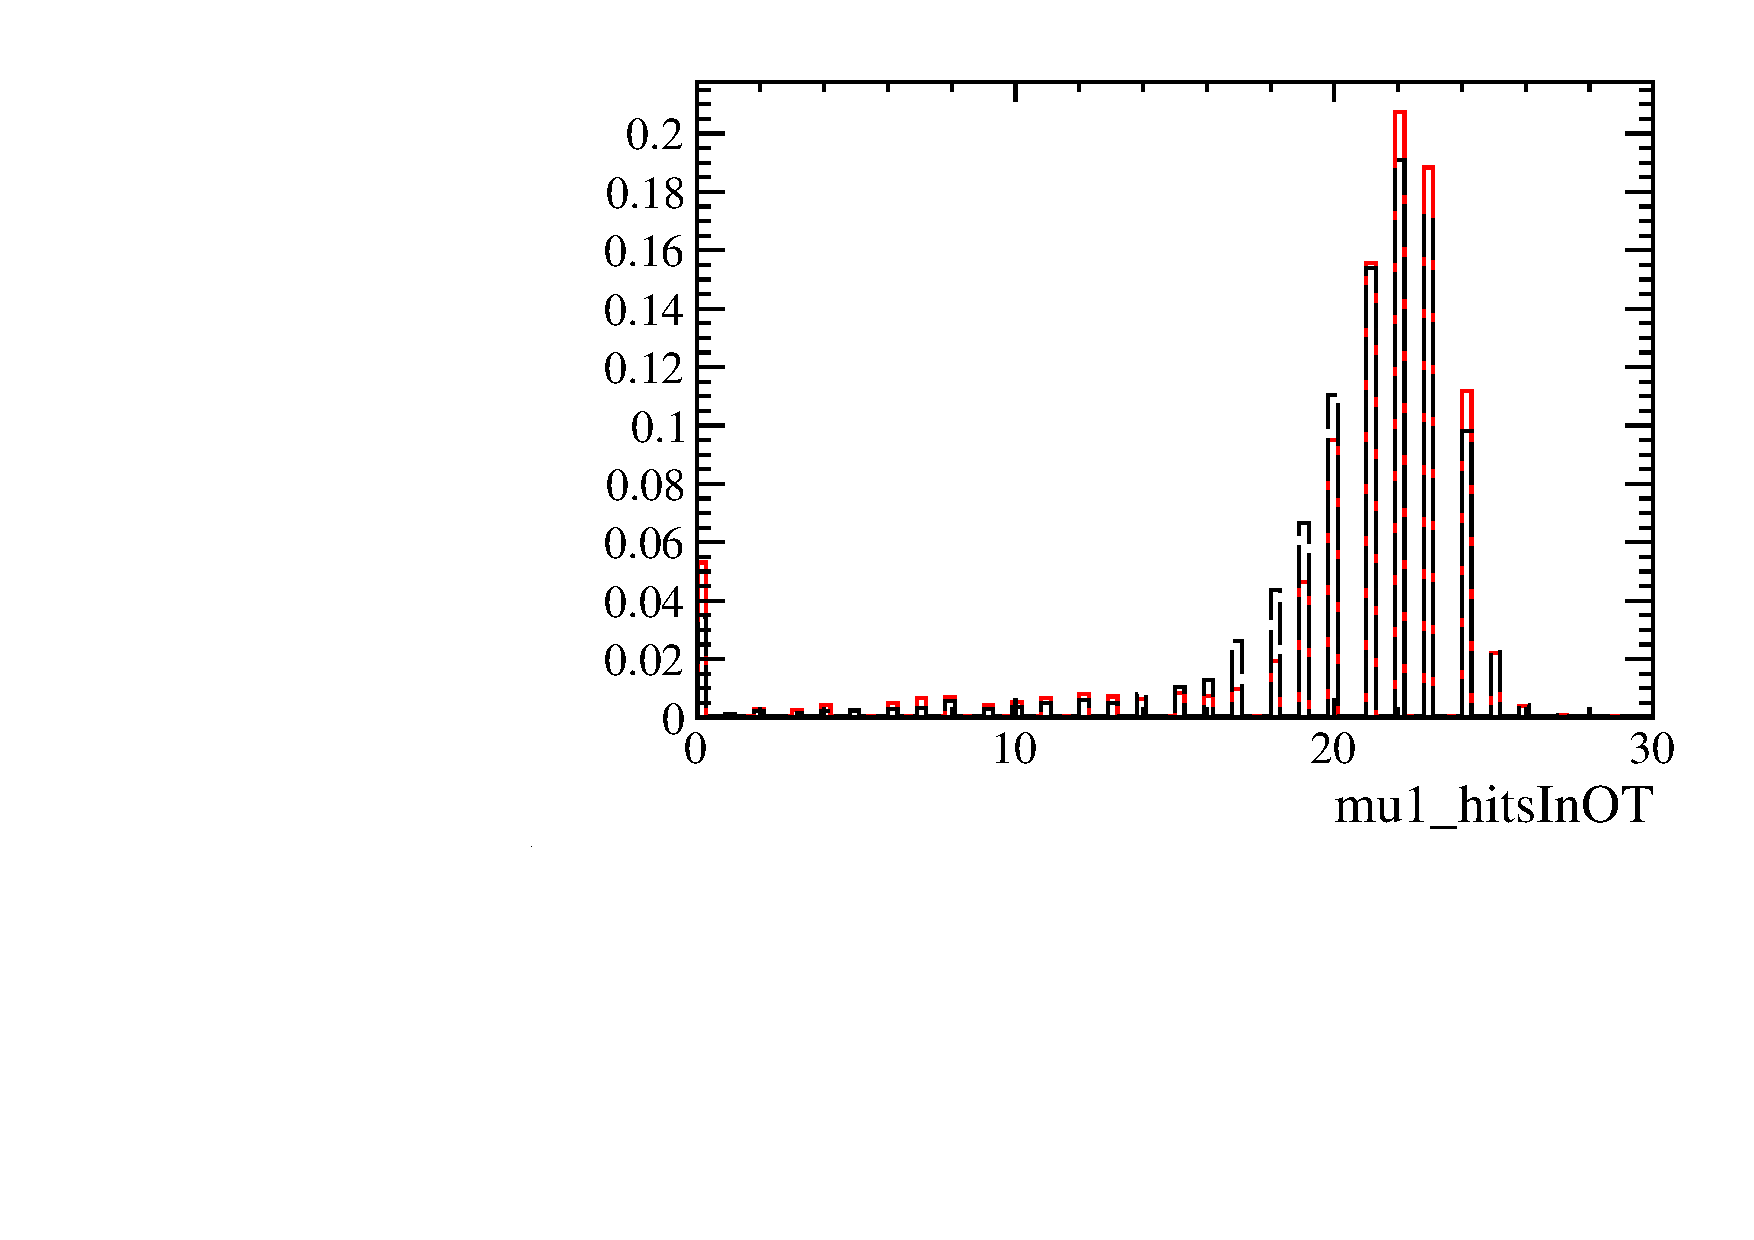
\includegraphics[scale=0.20]{figs/mu1_hitsInOTFULL.pdf}
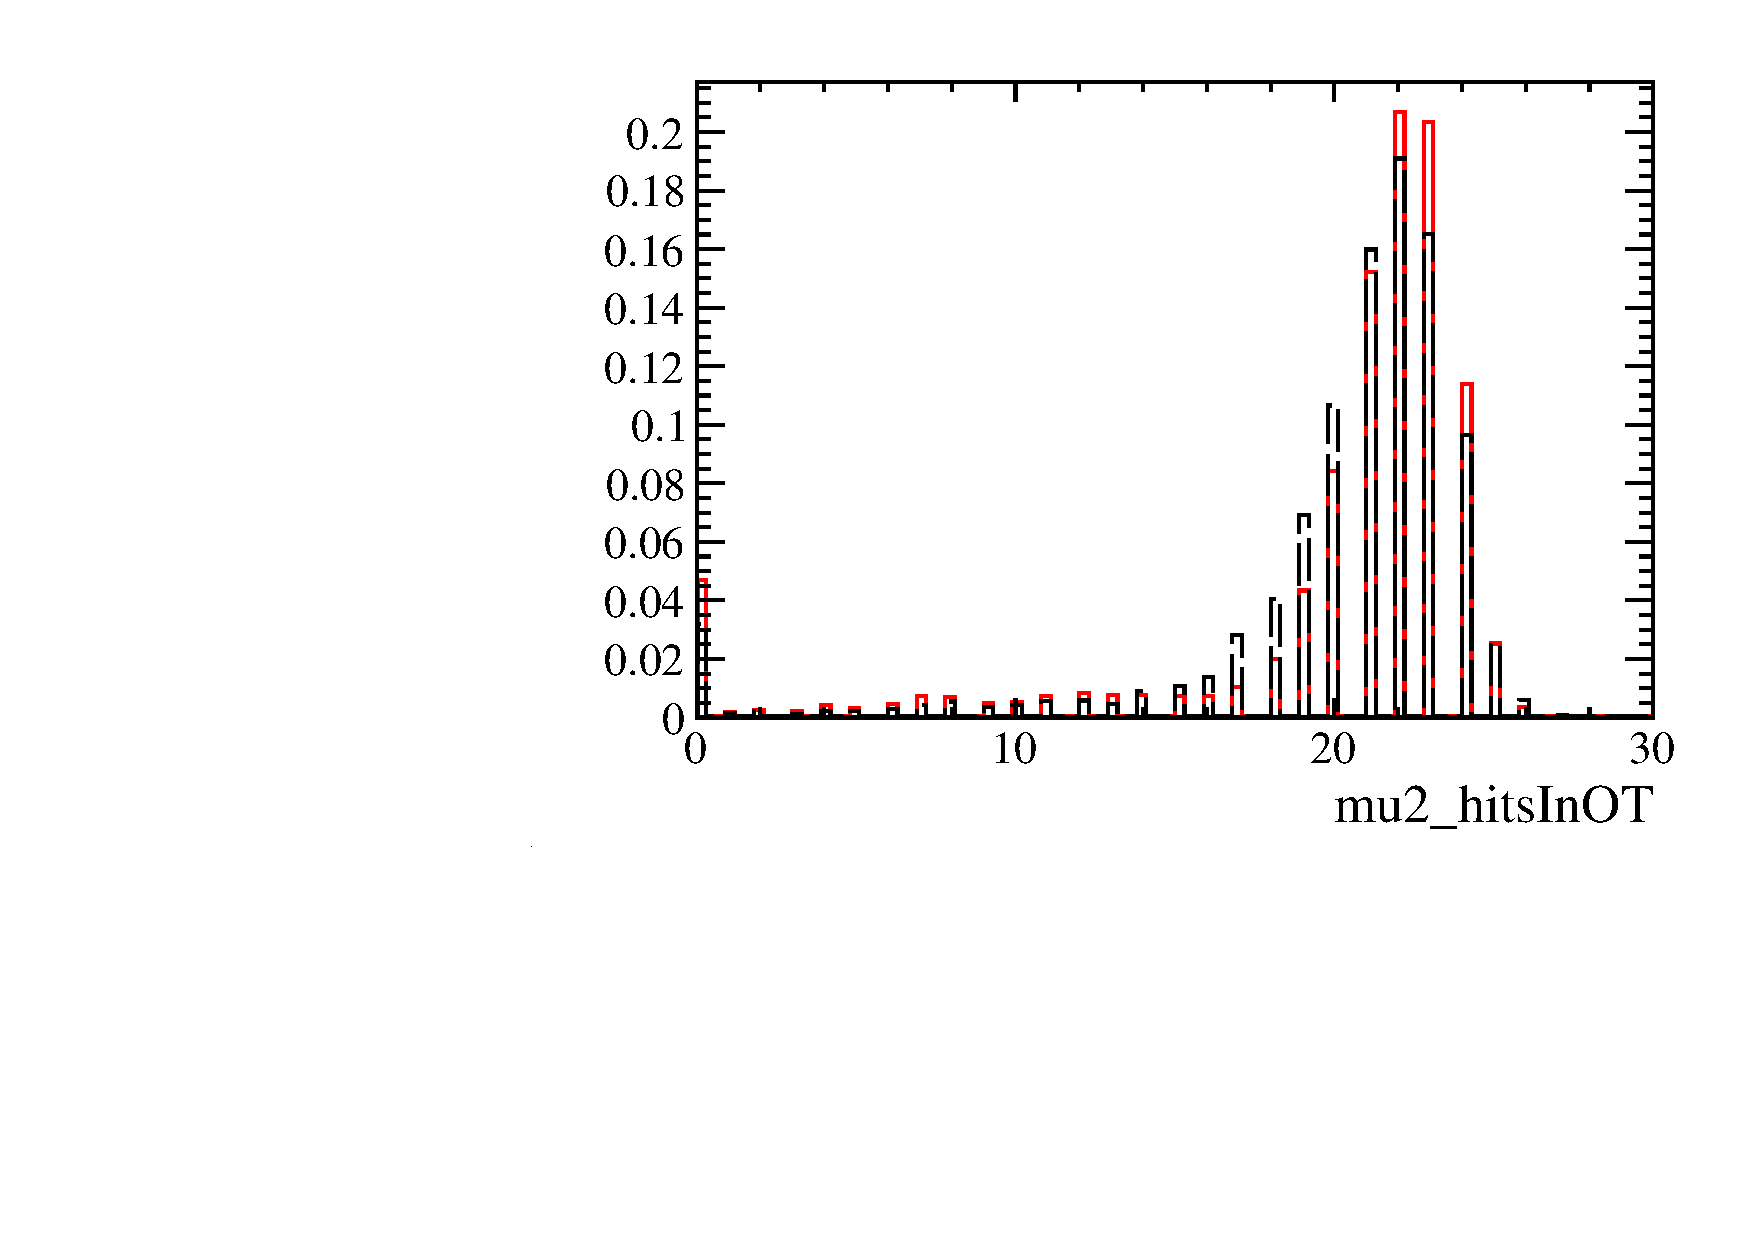
\includegraphics[scale=0.20]{figs/mu2_hitsInOTFULL.pdf}
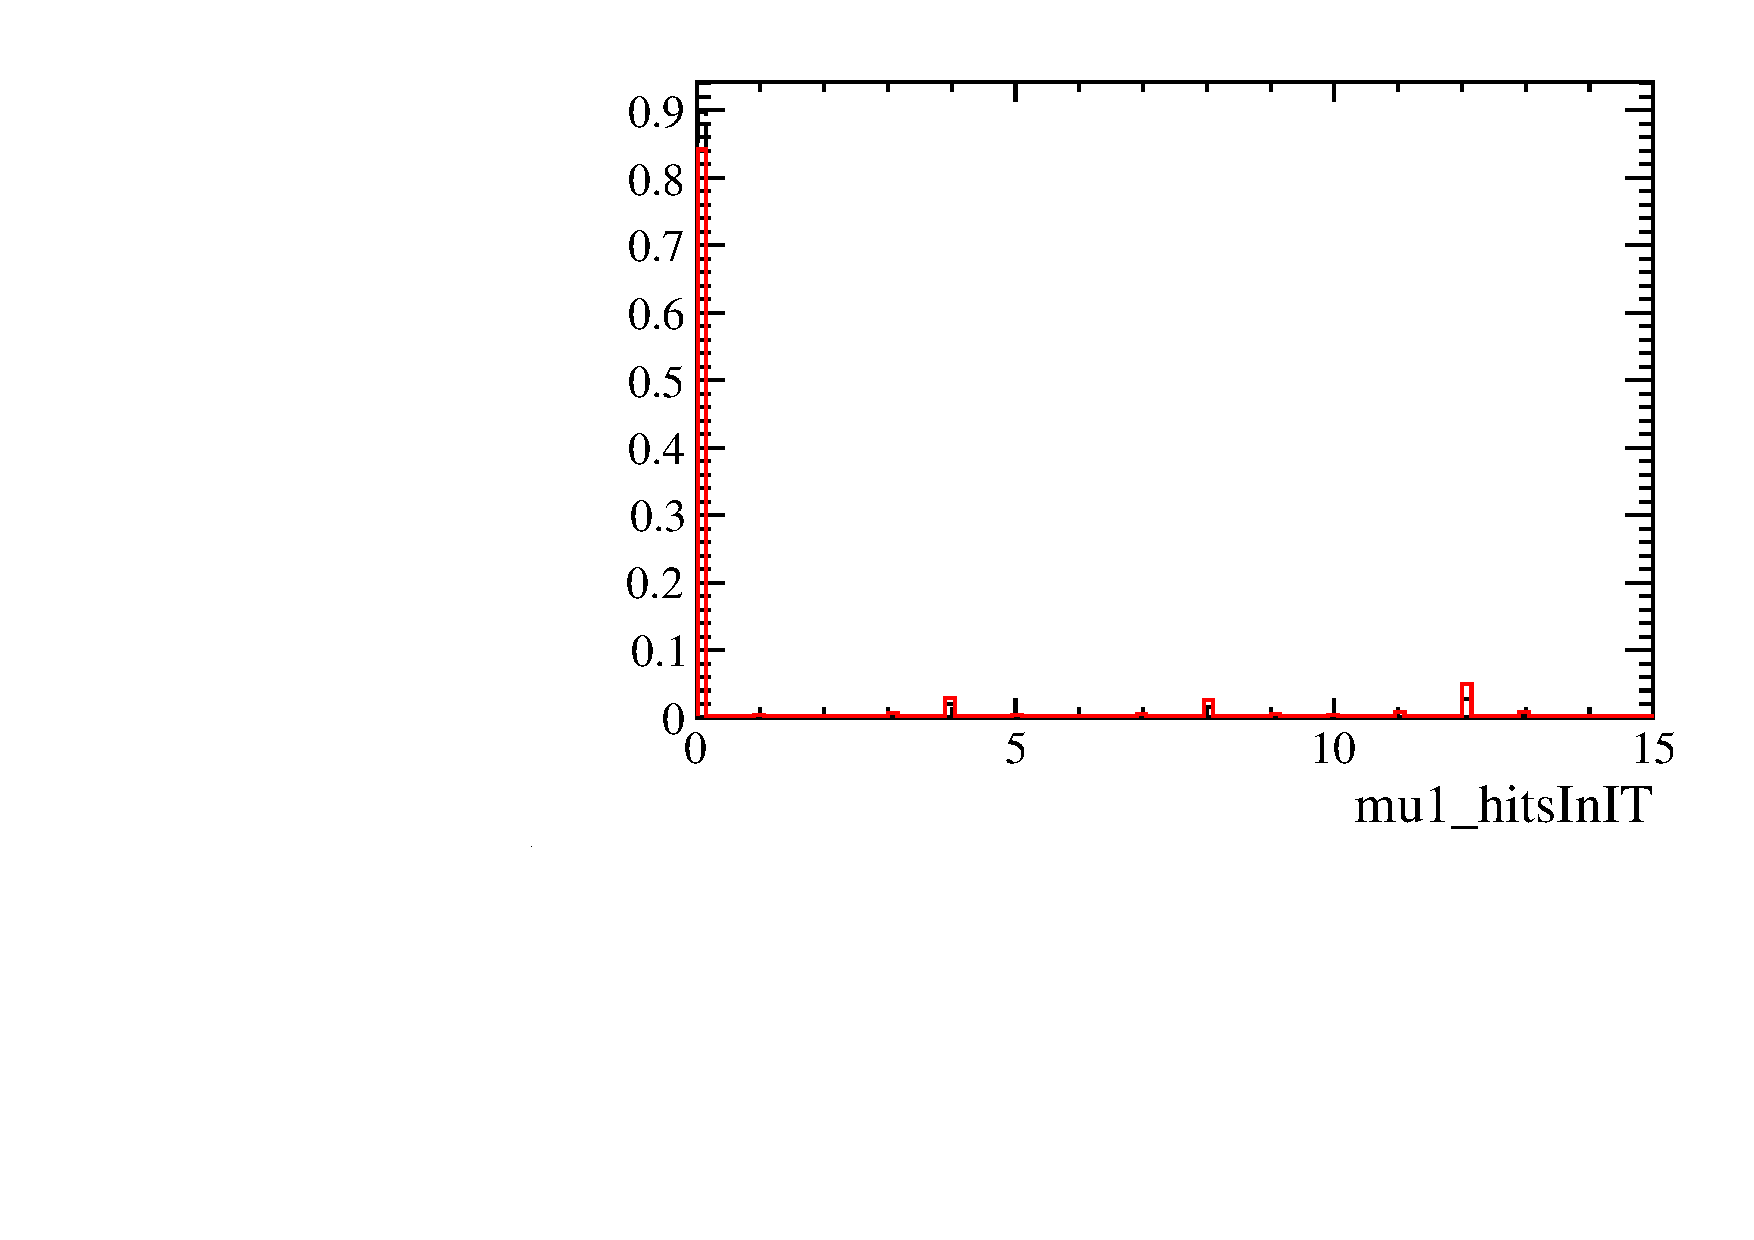
\includegraphics[scale=0.20]{figs/mu1_hitsInITFULL.pdf}
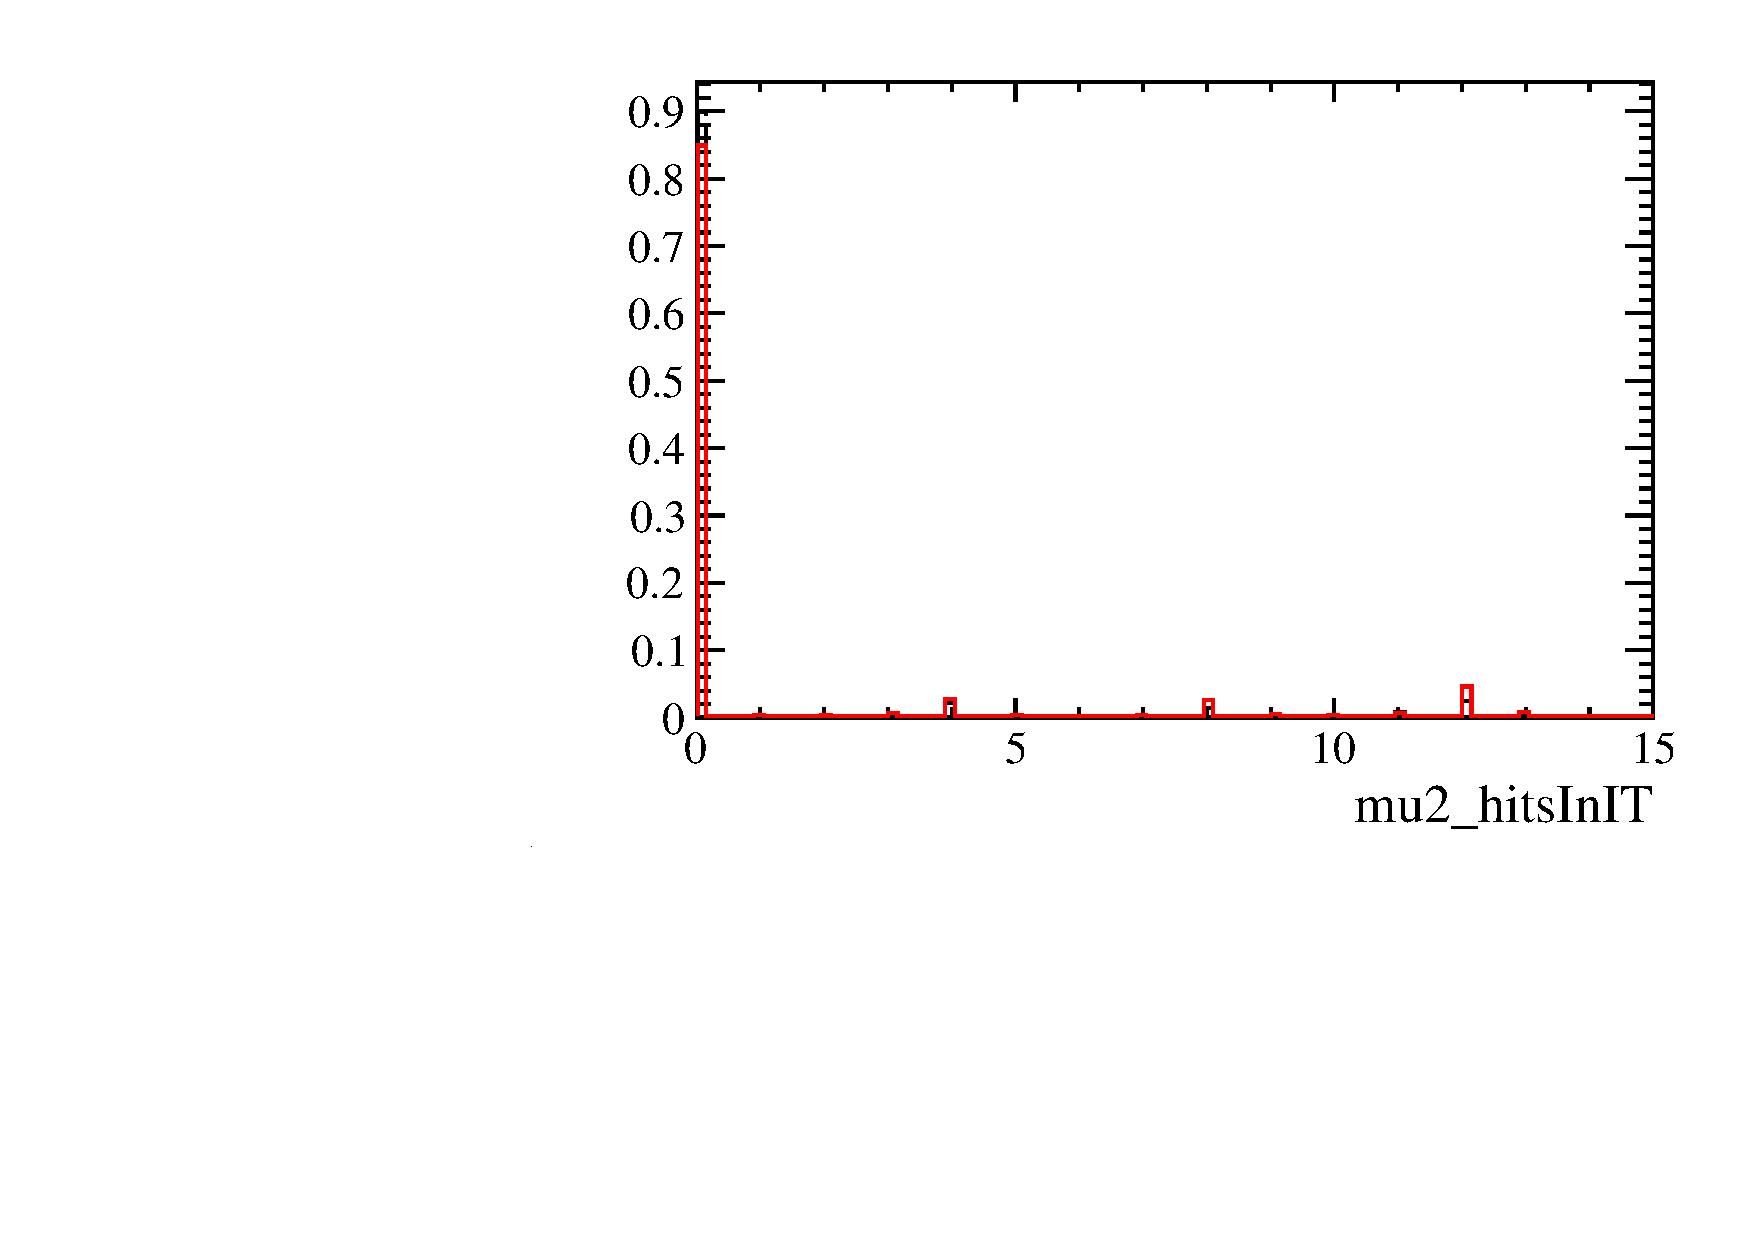
\includegraphics[scale=0.20]{figs/mu2_hitsInITFULL.pdf}
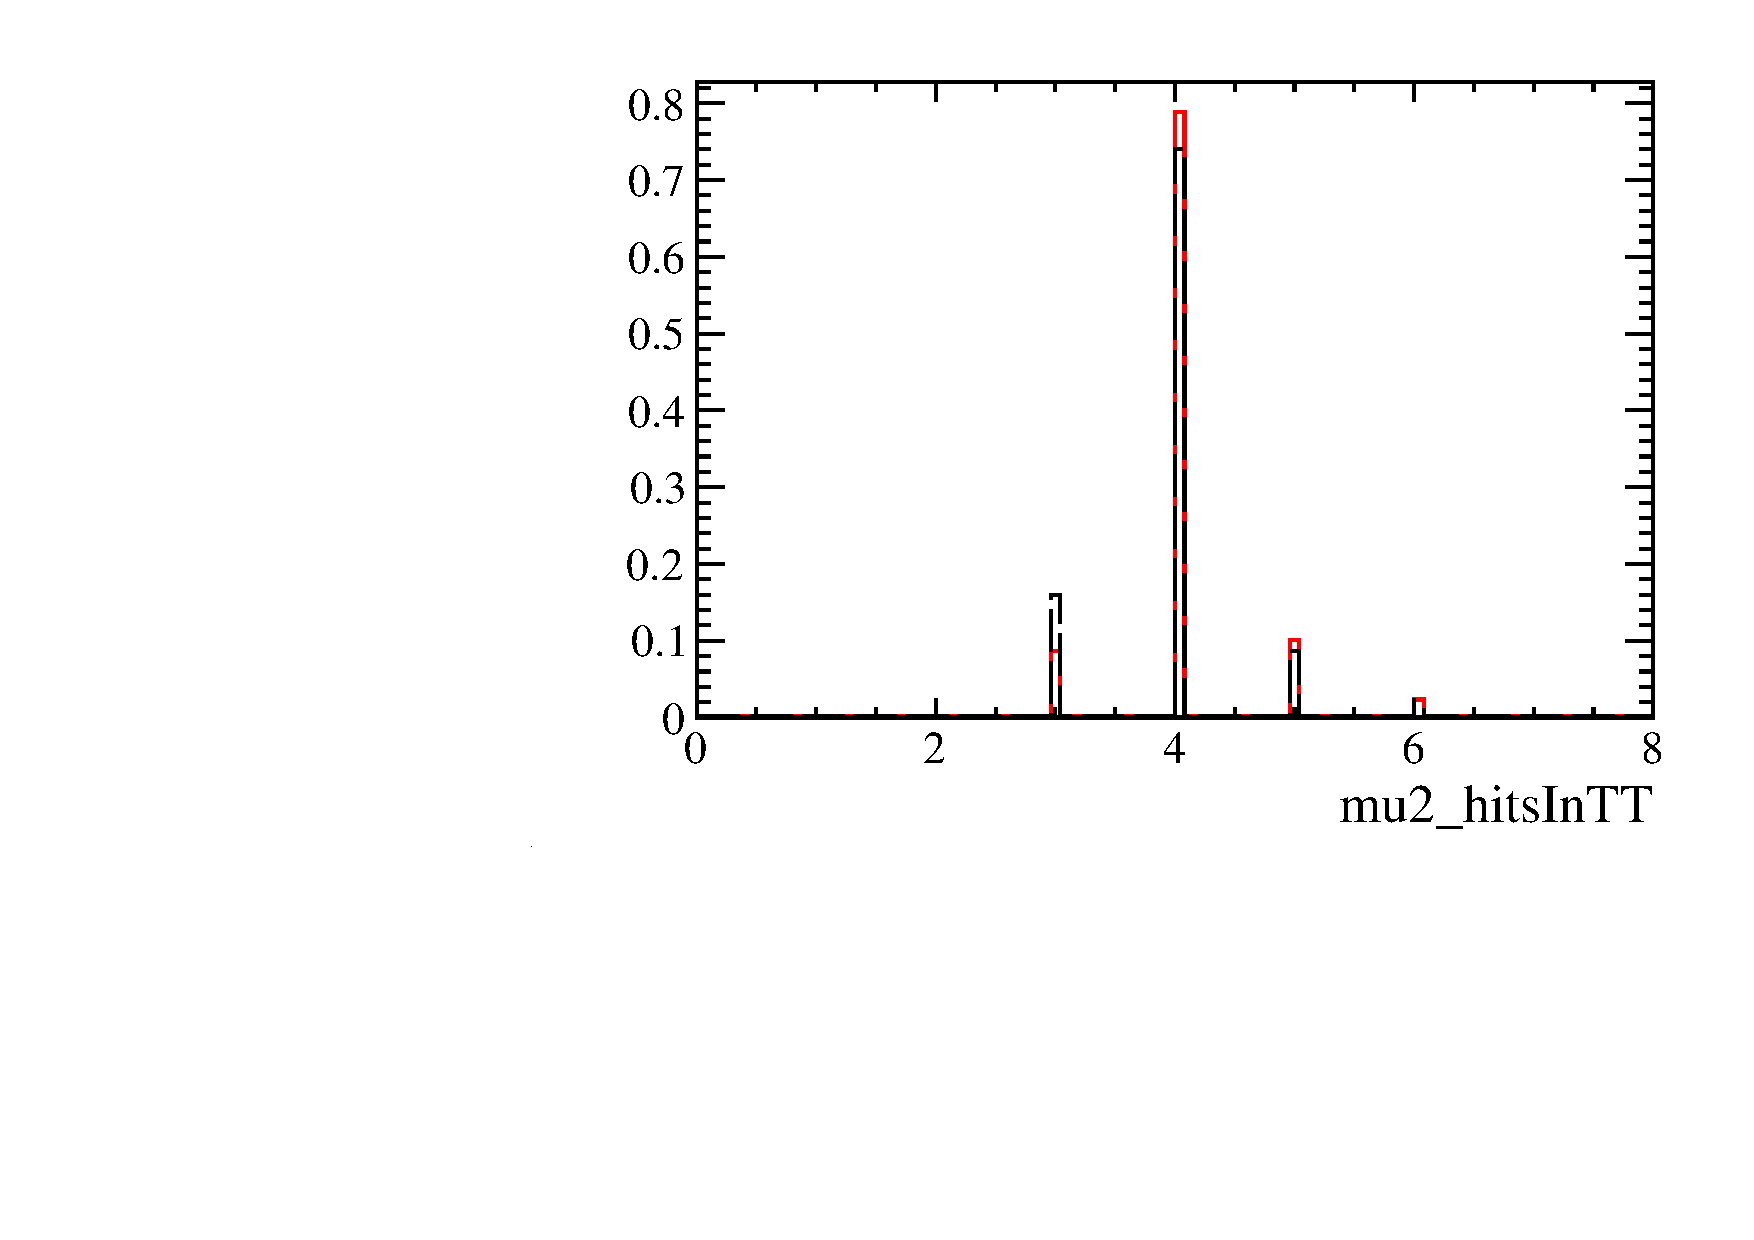
\includegraphics[scale=0.20]{figs/mu2_hitsInTTFULL.pdf}
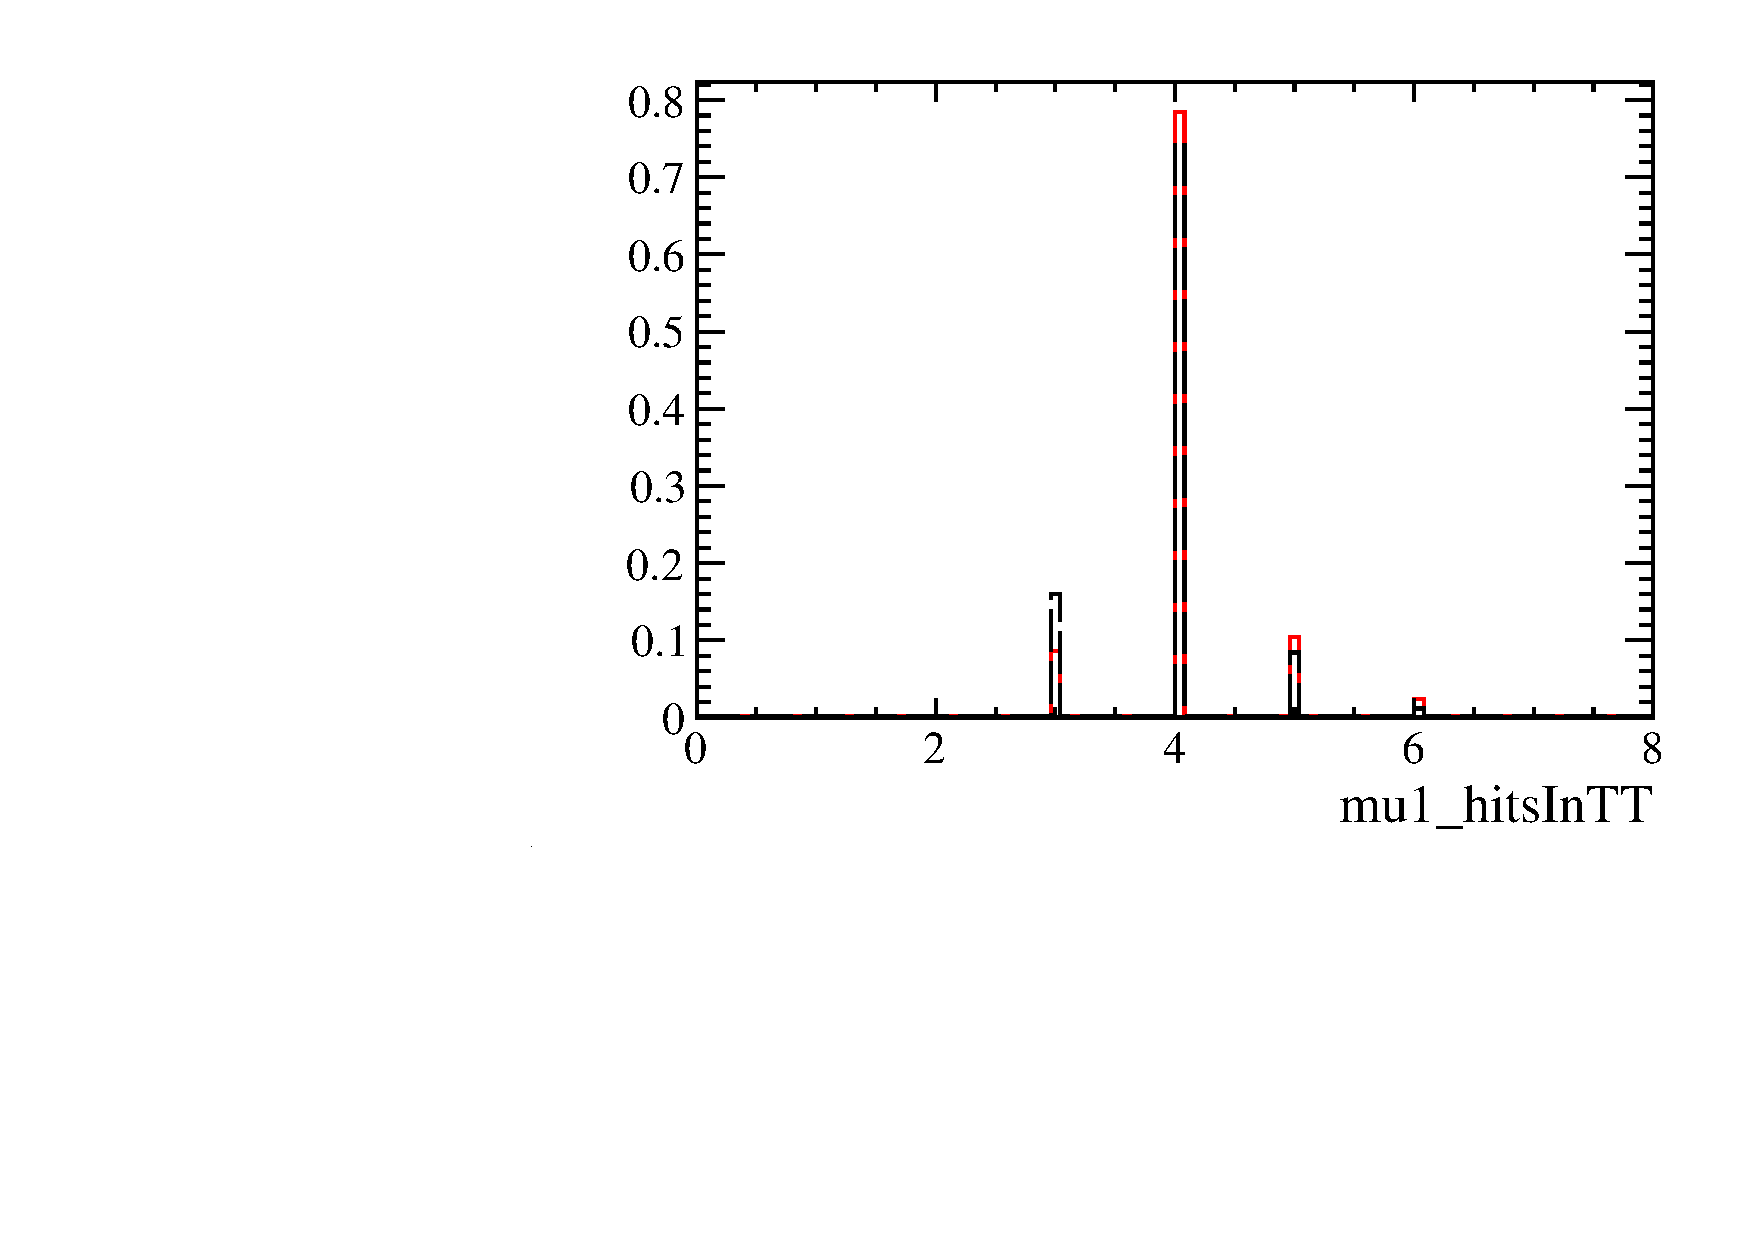
\includegraphics[scale=0.20]{figs/mu1_hitsInTTFULL.pdf}
\caption{Input variable distributions for signal (red) and background (black) for the FULL case. \label{fig:MVAhistos_FULL1}}
\end{center}
\end{figure}

\begin{figure} [htb!]
\begin{center}
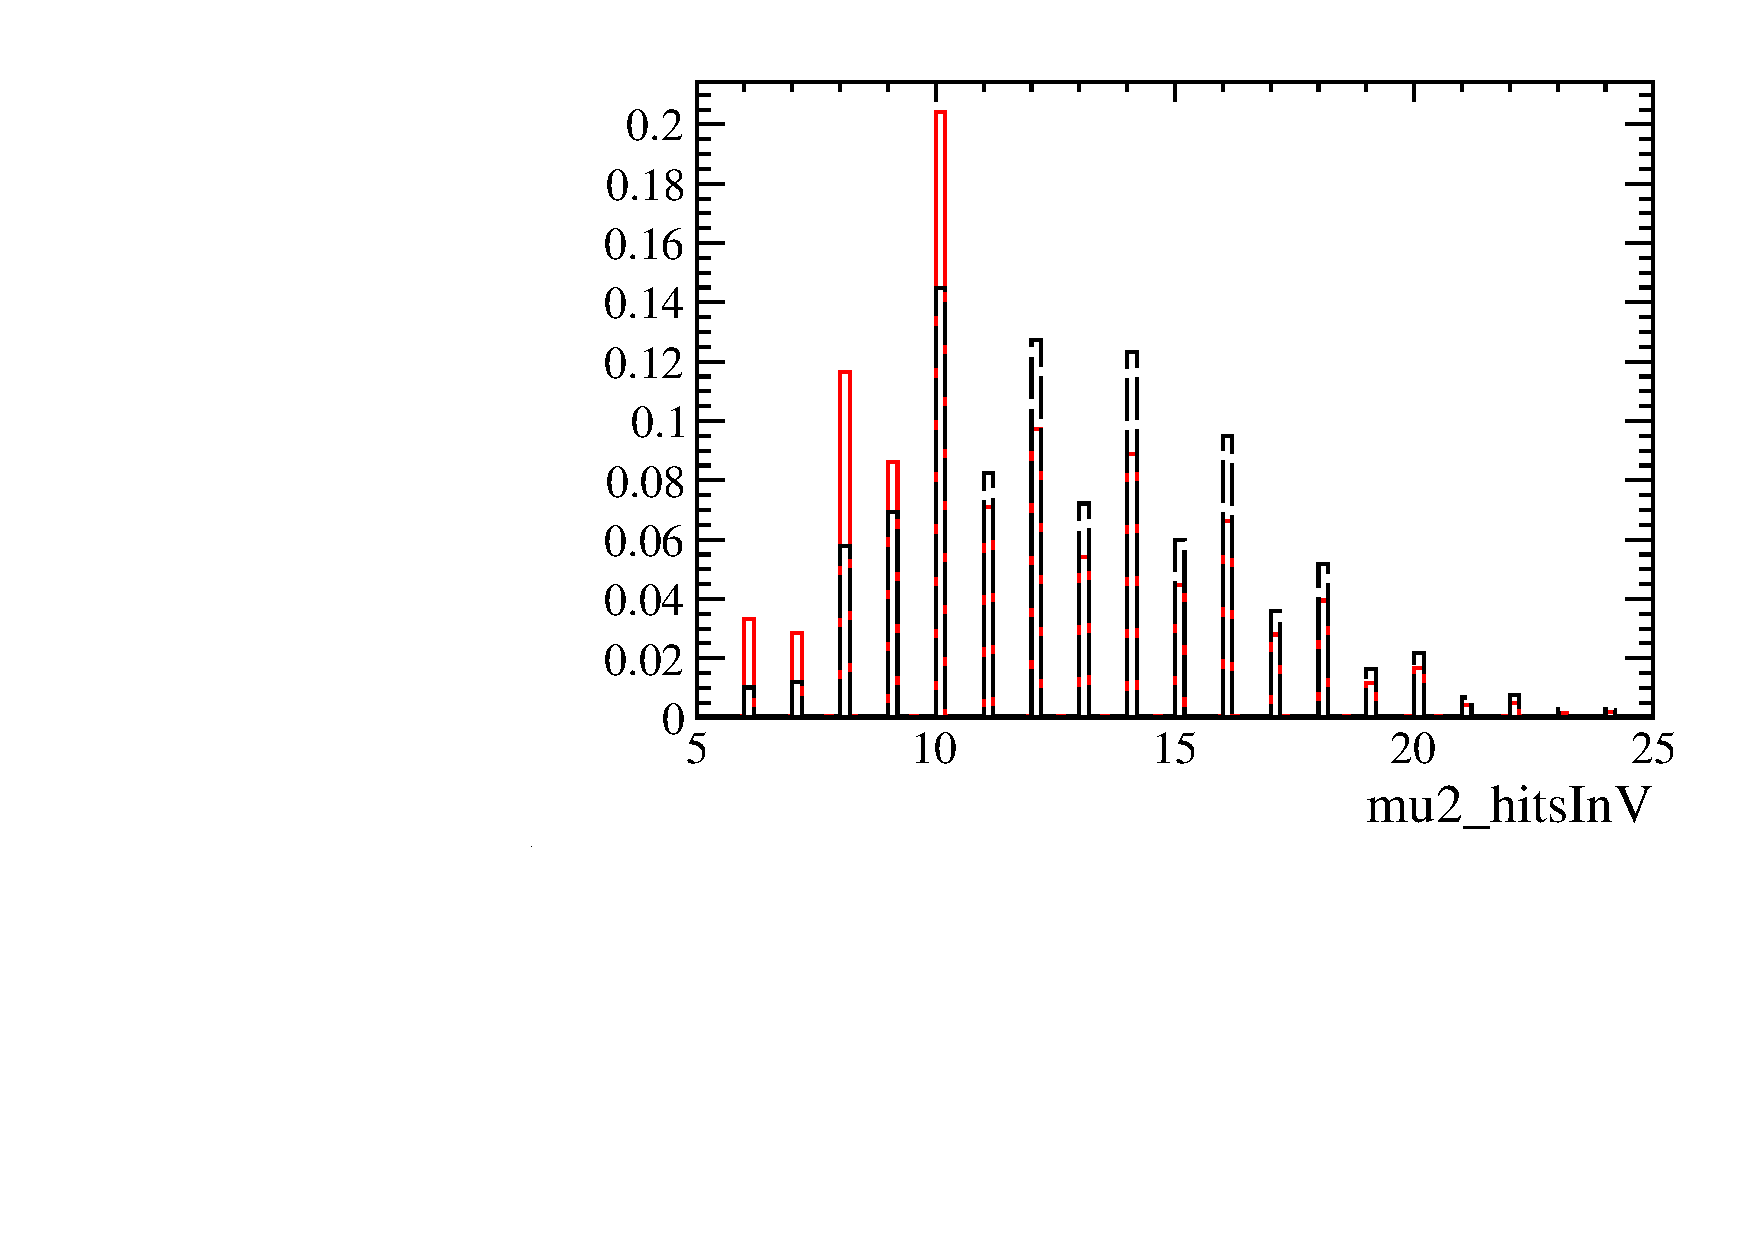
\includegraphics[scale=0.20]{figs/mu2_hitsInVFULL.pdf}
\includegraphics[scale=0.20]{figs/mu1_hitsInVFULL.pdf}
\includegraphics[scale=0.20]{figs/SV1FULL.pdf}
\includegraphics[scale=0.20]{figs/SV2FULL.pdf}
\includegraphics[scale=0.20]{figs/SV3FULL.pdf}
\caption{Input variable distributions for signal (red) and background (black) for the FULL case. \label{fig:MVAhistos_FULL2}}
\end{center}
\end{figure}

\begin{figure} [htb!]
\begin{center}
\includegraphics[scale=0.20]{figs/DOCAPARTIAL.pdf}
\includegraphics[scale=0.20]{figs/mu1ipsPARTIAL.pdf}
\includegraphics[scale=0.20]{figs/mu2ipsPARTIAL.pdf}
\includegraphics[scale=0.20]{figs/BipsPARTIAL.pdf}
\includegraphics[scale=0.20]{figs/BptPARTIAL.pdf}
\includegraphics[scale=0.20]{figs/BdissigPARTIAL.pdf}
\includegraphics[scale=0.20]{figs/PIDmu1PARTIAL.pdf}
\includegraphics[scale=0.20]{figs/PIDmu2PARTIAL.pdf}
\includegraphics[scale=0.20]{figs/Vchi2PARTIAL.pdf}
\includegraphics[scale=0.20]{figs/mu1_track_Chi2DoFPARTIAL.pdf}
\includegraphics[scale=0.20]{figs/mu2_track_Chi2DoFPARTIAL.pdf}
\includegraphics[scale=0.20]{figs/mu1_hitsInOTPARTIAL.pdf}
\includegraphics[scale=0.20]{figs/mu2_hitsInOTPARTIAL.pdf}
\includegraphics[scale=0.20]{figs/mu2_hitsInITPARTIAL.pdf}
\includegraphics[scale=0.20]{figs/mu1_hitsInITPARTIAL.pdf}
\includegraphics[scale=0.20]{figs/mu1_hitsInTTPARTIAL.pdf}
\includegraphics[scale=0.20]{figs/mu2_hitsInTTPARTIAL.pdf}
\includegraphics[scale=0.20]{figs/mu1_hitsInVPARTIAL.pdf}
\includegraphics[scale=0.20]{figs/mu2_hitsInVPARTIAL.pdf}
\includegraphics[scale=0.20]{figs/SV1PARTIAL.pdf}
\includegraphics[scale=0.20]{figs/SV2PARTIAL.pdf}
\includegraphics[scale=0.20]{figs/SV3PARTIAL.pdf}
\caption{Input variable distributions for signal (red) and background (black) for the PARTIAL case.
\label{fig:MVAhistos_PARTIAL}}
\end{center}
\end{figure}




%% $Id: introduction.tex 87303 2016-02-08 13:44:29Z lafferty $
\clearpage
\newpage
\section{Appendix: Samples used}
\label{sec:samples}
%{\it Miriam fill this}

The results described in this note were obtained using the data collected by LHCb at the LHC at a centre-of-mass energies of $\sqrt{s} = 7, 8 \text{ and } 13 \tev$ during the years 2011, 2012, and 2016, 
respectively. Both positive ($B_y > 0$) and negative ($B_y < 0$) magnet polarities are considered. 
%The data were reconstructed in the Reco14 framework using Brunel [7] v43r2p2, with
%the Condition Data Base [8] (condDB) tag cond-20121025 and the Detector Data Base [9]
%(DDDb) tag dddb-20120831. They were stripped with the Stripping20p3 reconstruction
%campaign, using DaVinci [10] v32r2p14.

Two separate stripping lines, described in \secref{app:selection}, are used for the FULL and PARTIAL categories. Note that in both cases that two different stripping lines are used for \Kspizmm and \Kspipi.
They are part of the LEPTONIC(MDST) stream for the Stripping 21 and DIMUON(DST) stream for the Stripping 24 and Stripping 26. \\
The following samples were used for the preparation of this note:
\begin{itemize}
\item Signal MC samples:
\begin{itemize}
%\item Event type 30000000, using the Sim08f configuration for the 2012 conditions. Reco14a framework, Stripping 20 NoPrescalingFlaggedALLSTREAMS
%\item Event type 34112401, using the Sim08c configuration for the 2012 conditions. Reco14a framework, Stripping 20 NoPrescalingFlaggedALLSTREAMS
\item Event type 34112407, using the Sim09a configuration for the 2012 conditions. Reco14c framework,condB tag~\cite{condDB} sim-20160321-2-vc-md100 (magnet down) and sim-20160321-2-vc-mu100 (magnet up), Detector Data base tag~\cite{dddb} dddb-20150928, Stripping 21 Filtered. %MC12
\item Event type 34102408, using the Sim09a configuration for the 2012 conditions. Reco14c framework,condB tag~\cite{condDB} sim-20160321-2-vc-md100 (magnet down) and sim-20160321-2-vc-mu100 (magnet up), Detector Data base tag~\cite{dddb} dddb-20150928, Stripping 21 Filtered. %MC12 bkg
\item Event type 34112407, using the Sim09a configuration for the 2015 conditions. Reco15a framework,condB tag~\cite{condDB} sim-20160606-vc-md100 (magnet down) and sim-20160606-vc-mu100 (magnet up), Detector Data base tag~\cite{dddb} dddb-20150724, Stripping 24 NoPrescalingFlagged. %MC15
%\item Event type 34112401, using the Sim08e configuration for the 2012 conditions. Reco14a framework, Stripping 20 NoPrescalingFlagged
\end{itemize}



%\begin{itemize}
%\item Stat,Generation Cuts, Stat to disk, Stat stripped (?)
%\end{itemize}
%Brunel ~\cite{brunel}
%condDB ~\cite{condDB}
%DDDb ~\cite{dddb}
%DaVinci ~\cite{DaVinci}
%Erasmus ~\cite{Erasmus}
\item Stripping 21 data.
\begin{itemize}
%\item Reco14 framework, Brunel~\cite{brunel} v43r2p2, condB tag~\cite{condDB} cond-20130114, Detector Data base tag~\cite{dddb} dddb-20130111. Stripping 21r1, DaVinci~\cite{DaVinci} v36r1. 
%Data from 2011 collisions, $0.992 \pm 0.001 \;\invfb$.
%\item Reco14 framework, Brunel~\cite{brunel} v43r2p2, condB tag~\cite{condDB} dddb-20120831, Detector Data base tag~\cite{dddb} dddb-20120831. Stripping 21, DaVinci~\cite{DaVinci} v36r1. 
%Data from 2012 collisions, $2.036 \pm 0.002 \;\invfb$.
\item Reco14 framework, Brunel~\cite{brunel} v43r2p2, condB tag~\cite{condDB} cond-20141107, Detector Data base tag~\cite{dddb} dddb-20130929. Stripping 21r1, DaVinci~\cite{DaVinci} v36r1. 
Data from 2011 collisions, $0.992 \pm 0.001 \;\invfb$.
\item Reco14 framework, Brunel~\cite{brunel} v43r2p2, condB tag~\cite{condDB} cond-20141107, Detector Data base tag~\cite{dddb} dddb-20130929-1. Stripping 21, DaVinci~\cite{DaVinci} v36r1. 
Data from 2012 collisions, $2.036 \pm 0.002 \;\invfb$.


\end{itemize}
% \item Stripping 24 data, 0.132 $fb^{-1}$.
% \begin{itemize}
% \item Reco15a framework, Brunel~\cite{brunel} v47r8, condB tag~\cite{condDB} cond-20150828, Detector Data base tag~\cite{dddb} dddb-20150724. Stripping 24, DaVinci~\cite{DaVinci} v38r1p1. Data from 2015 collisions.
% \end{itemize}
\item Stripping 26 data.
\begin{itemize}
\item Reco16 framework, Brunel~\cite{brunel} v47r8, condB tag~\cite{condDB} cond-20160522, Detector Data base tag~\cite{dddb} dddb-20150724. Stripping 26, DaVinci~\cite{DaVinci} v40r2p1. 
Data from 2016 collisions, $0.306 \pm 0.001 \;\invfb$.
\end{itemize}
\end{itemize}






%% $Id: introduction.tex 87303 2016-02-08 13:44:29Z lafferty $
\clearpage
\newpage
\section{Appendix: Normalization}
\label{app:normalization}

The signal yield is normalised with respect to \Kspipi . The yield is computed as follows:
\begin{equation}
N(\KsPzMuMu) = \sigma(\PKzS){\cal B}(\KsPzMuMu)\epsilon_{\KsPzMuMu} L,
\end{equation}
where $\sigma(\PKzS)$ is the \KS production cross-section, $\epsilon_{\KsPzMuMu}$ the absolute efficiency and $L$ the integrated luminosity. Taking the ratio of N(\KsPzMuMu) with respect to N(\Kspipi), both the 
cross-section and the luminosity get cancelled out, leading to the formula:

\begin{equation}
\frac{N(\KsPzMuMu)}{N(\Kspipi)} = \frac{\BRof\KsPzMuMu}{\BRof\Kspipi} \frac{\epsilon_{\KsPzMuMu}}{\epsilon_{\PKzS\to\Pgpp\Pgpm}}.
\end{equation}

The effective luminosity, $L^{dat}_{eff}$, is calculated according to

\begin{equation}
L^{dat}_{eff} = \epsilon^{TIS}_{\Kspipi}L^{dat}, \\
\end{equation}	
where $\epsilon_{TIS}(\Kspipi)$ is the TIS efficiency calulated using \Kspipi events and $L^{dat}$ is the luminosity used for the fit to the data.

\begin{eqnarray}
L^{FULL,2011}_{eff} &=& 0.0016 \cdot 992\;\rm pb^{-1} = 1.59\;\invpb, \\
L^{FULL,2012}_{eff} &=& 0.0016 \cdot 2037\;\rm pb^{-1} = 3.26\;\invpb,\\
L^{PARTIAL}_{eff} &=& 0.0025 \cdot 306\;\rm pb^{-1} = 0.77\;\invpb. 
\end{eqnarray}

The offline signal efficiency (or, equivalently, the total efficiency for a $100\%$ efficient trigger) for the FULL channel is calculated as follows:
\begin{itemize}

\item The generator level efficiency is estimated to be $0.361$. 
\item The efficiency of the FULL stripping on generated events is $1.84$ per mil according to the statistics produced by the DaVinci filtering script. This number has to be corrected by the fact that $3.3\%$ of the events didn't actually contain a signal candidate at all \footnote{In a fraction of events, the information on how the \KS should decay is lost as the particle is passed to GEANT4.}. It also has to be corrected by the fact that some of the selected candidates aren't matched to the signal. After this corrections, it becomes $1.79$ per mil.
\item The efficiency of the fiducial cuts  and mass fit window are $0.931$ and $0.922$. These are applied prior to BDT training.
\end{itemize}

The offline signal efficiency (or, equivalently, the total efficiency for a $100\%$ efficient trigger) for the PARTIAL channel is calculated as follows:
\begin{itemize}

\item The generator level efficiency is estimated to be $0.361$. 
\item The efficiency of the PARTIAL stripping on generated events, calculated in the same way as above is $1.23\%$.
\item The efficiency of the fiducial cuts  and mass fit window are $0.734$ and $0.917$ respectively. These are applied prior to BDT training.
\end{itemize}

%% $Id: introduction.tex 87303 2016-02-08 13:44:29Z lafferty $
\clearpage
\newpage

\section{Appendix: Peaking background studies}
\label{app:background}

%{\it Give details on the \KL supression factor and on the \KLTpi}

The upper decay time acceptance (mainly the limited size of the VELO) causes the \KL reconstruction efficiency to be much lower than that of the \KS by about a factor of thousand ~\cite{KsmmANA}. We checked that a similar 
factor applies to our decay. Indeed, repeating the calculations of Sect.~6 in Ref.~\cite{KsmmANA} using our measured value of $\alpha_{\Kspizmm} = -110.9\pm 1.2 \; \rm ns^{-1}$ (see \figref{fig:lifetime}), we recovered an efficiency 
ratio factor of $\approx 2.2\times10^{-3}$.

\begin{figure} [htb!]
\begin{center}
\includegraphics[scale=0.3]{figs/lifetime.pdf}
%\includegraphics[scale=0.30]{figs/mK3pi_PARTIAL_wKsPiPi.pdf}
\caption{Lifetime distribution of selected \Kspizmm for $t>8.95\;\rm ps$. The red line shows an exponential fit, used to obtain $\alpha$~\cite{KsmmANA}. \label{fig:lifetime}}
\end{center}
\end{figure}


Samples of $K^0_S\rightarrow\pi^+\pi^-\pi^0$ corresponding to event type 34102408 were generated in order to study the \KLTpi  background.
The invariant mass distribution of the events stripped in a sample of $K^0_S\rightarrow\pi^+\pi^-\pi^0$ is shown in \figref{fig:KLTpi_wKspipi}. 
It can be seen as the right hand side bump (see also \figref{fig:mumuKspipi}) where we also included the \Kspipi from the underlying event and that also pass the selection. 
The Ismuon requirement was dropped from the stripping to increase the statistics. We find 254 \Kspipi out of 735 candidates. Taking into account the suppresion factor for \KL to \KS ($\sim2\times10^{-3}$), 
the MC generation efficiency ($\approx 0.36$) and the fact that the $3\pi$ decays is forced, we expect a ratio of $\sim2\times10^{-4}$ \KLTpi per \Kspipi decay in our PARTIAL background. 
A stripping 21 (i.e, FULL) filtered \KSTpi sample is also available. In that case we find about $50\%$  of the events actually come from the forced decay. Again, taking into account the \KL to \KS supression factor, 
we find that this background is small compared to other sources. The BDT and mass distributions of the 18 events of the filtered sample which also pass the selection cuts applied prior to BDT training is shown in 
\figref{fig:KLTpi_BDT}. No events are in the BDT region used for the fit, and the effective luminosity of the sample is insufficient to derive a meaningful quantitative upper limit on the number of \KLTpi events expected 
in the data. Finally, in order to asess the possible impact on the sensitivity, we add to the fit a Landau component with parameters fixed to those obtained from simulation at the stripping filtered level (we lack 
statistics to do it after all cuts and per BDT bin), as shown in \figref{fig:Landau}. The fit to data is shown in \figref{fig:fitK3pi}. The expected sensitivity for 50 fb$^{-1}$ including this component is 
$\pm5.3\times10^{-9}$, very similar to the one obtained when this component is ignored, $5.5\times10^{-9}$. The size of the Landau component is consistent with zero at one sigma in all BDT bins.


   
To study the contribution of a background due to three-pion final state decays, such as $\eta\to\pi^+\pi^-\pi^0$, the invariant $K^{0}$ mass is reconstructed using the pion mass hypothesis
for the muons. The corresponding distributions are shown in \figref{fig:eta_bkg}. No peaking structures in the signal region are to be seen.
   
\begin{figure} [htb!]
\begin{center}
\includegraphics[scale=0.60]{figs/M_V0_K3pi_Kspipi.pdf}%{figs/mK3pi_PARTIAL_wKsPiPi.pdf}
%\includegraphics[scale=0.30]{figs/mK3pi_PARTIAL_wKsPiPi.pdf}
\caption{Invariant mass distribution of simulated $K^0\rightarrow\pi^+\pi^-\pi^0$ decays selected in the PARTIAL category including also the \Kspipi decays that got selected from the underlying event, 
which can be seen as the right hand side bump. \label{fig:KLTpi_wKspipi}}
\end{center}
\end{figure}
   
\begin{figure} [htb!]
\begin{center}
\includegraphics[scale=0.60]{figs/M_mumu_K3pi_Kspipi.pdf}%{figs/mumu_mass.pdf}
%\includegraphics[scale=0.30]{figs/mumu_mass.pdf}
\caption{Invariant mass distribution of dimuon candidates in simulated $K^0\rightarrow\pi^+\pi^-\pi^0$ decays selected in the PARTIAL category, and including also the \Kspipi that got selected from the underlying event. 
\label{fig:mumuKspipi}}
\end{center}
\end{figure}

\begin{figure} [htb!]
\begin{center}
\includegraphics[scale=0.3]{figs/filtered_mass_BDTintegrated.pdf}
\includegraphics[scale=0.30]{figs/K3pi_BDT.pdf}
\caption{Mass and BDT distribution of the \KSTpi simulated FULL candidates.\label{fig:KLTpi_BDT}}
\end{center}
\end{figure}
\begin{figure} [htb!]
\begin{center}
\includegraphics[scale=0.6]{figs/landau.pdf}
\caption{Mass of \KSTpi after stripping FULL, and fit to a Landau \pdf. \label{fig:Landau}}
\end{center}
\end{figure}

\begin{figure} [htb!]
\begin{center}
\includegraphics[scale=0.5]{figs/fit_wK3pi.pdf}
%\includegraphics[scale=0.30]{figs/K3pi_BDT.pdf}
\caption{Fit to the dataset FULL including a Landau component for \KLTpi. The size of the Landau component is consistent with zero at one sigma in all BDT bins. \label{fig:fitK3pi}}
\end{center}
\end{figure}


\begin{figure} [htb!]
\begin{center}
\includegraphics[scale=0.30]{figs/M_VC_pipi_hyp.pdf}
\includegraphics[scale=0.30]{figs/M_V0_pipi_hyp.pdf}
\caption{Invariant $\pi^{+}\pi^{-}\pi^0$ mass distribution of kaon candidates in decays in the FULL (left) and PARTIAL (right) data samples. The kaon mass is reconstructed using the pion mass hypothesis for the muons. \label{fig:eta_bkg}}
\end{center}
\end{figure}





%%% Paper 
\section{Probing SUSY effects in \KsMuMu}
In this section, the MSSM effects in the \KsMuMu decay are explored. The Standard Model (SM) expectation is $(5.18\pm 1.50_{\textrm{LD}} \pm 0.02_{\textrm{SD}})\times 10^{-12}$~\cite{Ecker:1991ru, Isidori:2003ts, DAmbrosio:2017klp}, where the first uncertainty comes from the long-distance (LD) contribution and the second one comes from the short-distance (SD) contribution. 
On the other hand, the current experimental upper bound is $8\times10^{-10}$ at $90\%$ C.L{.,} using $3$ fb${}^{-1}$ of LHCb data~\cite{LHCb:KsMuMu}. The LHCb upgrade could reach sensitivities at the level of about $1\times 10^{-11}$ or even below, approaching the SM prediction~\cite{DMS_FPCP}.
The branching ratio $\mathcal{B}(\KsMuMu)$ is predicted taking into account the relevant experimental constraints on the branching fractions $\mathcal{B}(K_L^0\rightarrow\mu^+\mu^-)$, $\mathcal{B}(B^+\rightarrow\tau^+\nu_{\tau})$ and $\mathcal{B}(K^+\rightarrow\mu^+\nu_{\mu})$, the $CP$ violation parameters $\varepsilon^{\prime}_K/\varepsilon_K$ and $\varepsilon_K$, the $K^{0}_{L}$--$K^{0}_{S}$ mass difference, $\Delta M_{K}\equiv M_{K^0_L} - M_{K^0_S}  > 0$, and the Wilson coefficient $C_7$ from $b\rightarrow s \gamma$. 
For this, the Mass Insertion Approximation (hereafter MIA)\cite{MassInsertion} is used, treating the corresponding terms as phenomenological parameters at the SUSY scale. The details of the formalism are given in subsection~\ref{subsec:formalism}. The subsets of the MSSM parameter space are studied in scans performed on Graphics Processing Units (GPU), as detailed in section~\ref{subsec:scan}. The results are shown in section~\ref{sec:results} and conclusions are drawn in section~\ref{subsec:conclusions}.

\subsection{Formalism}
\label{subsec:formalism}
The followed notation is the one of refs.~\cite{Altmannshofer:2009ne, Rosiek:1995kg}. The right-handed down and up squarks are denoted as $D$ and $U$, respectively. Because of the $\textrm{SU}(2)_{L}$ doublet, the two left-handed squarks are \red{degenerate}, and are denoted as $Q$. The average of the $Q$, $D$, and $U$-squark masses squared are denoted by $\tilde{m}^2_Q$, $\tilde{m}^2_d$, $\tilde{m}^2_u$, respectively.

The mass insertions (hereafter MIs) are defined as: 
\beq
\left( \delta_d^{LL}\right)_{ij} &=
\frac{ \left[ \left( \mathcal{M}_D^2 \right)_{LL} \right]_{ij}  }{\tilde{m}_{Q}^2} 
=  \frac{ ( m^2_{Q})_{ji}}{\tilde{m}_{Q}^2},\\
\label{eq:duLL}
\left( \delta_u^{LL}\right)_{ij} &=
\frac{ \left[ \left( \mathcal{M}_U^2 \right)_{LL} \right]_{ij}  }{\tilde{m}_{Q}^2} 
= \frac{ ( V m^2_{Q} V^{\dag} )_{ji}}{\tilde{m}_{Q}^2},\\
\left( \delta_d^{RR}\right)_{ij} &=
\frac{ \left[ \left( \mathcal{M}_D^2 \right)_{RR} \right]_{ij}  }{\tilde{m}_{d}^2} 
=  \frac{ ( m^2_{D})_{ij}}{\tilde{m}_d^2},
\eeq
where $V$ is the Cabibbo–Kobayashi–Maskawa (CKM) matrix and $\mathcal{M}^{2}_{D,U}$ are the $6\times 6$ squark mass matrices.
Note that the indices $ij$ are inverted for $LL$. Comparison with the SUSY Les Houches Accord 2 convention \cite{Allanach:2008qq} is given in the appendix of ref.~\cite{Altmannshofer:2009ne}.

The running coupling constants $\alpha_1$, $\alpha_2$, and $\alpha_3$ are defined as
\beq 
\label{eq:alphas}
\alpha_1 &= \frac{g_1^2}{4 \pi} = \frac{5}{3} \frac{g^{\prime 2}}{4 \pi}, \\
\alpha_2 &= \frac{g_2^2}{4 \pi} = \frac{g^2}{4 \pi}, \\
\alpha_3 &= \frac{g_3^2}{4 \pi} = \frac{g_s^2}{4 \pi},
\eeq 
where $g^{\prime}$, $g$, and $g_s$ are  the $\textrm{U}(1)_{Y}$, $\textrm{SU}(2)_{L}$, and  $\textrm{SU}(3)_{C}$ group coupling constants, respectively.	 In the following, these couplings are evaluated at the $\mu^{\textrm{SUSY}}$ scale, defined as $\mu^{\textrm{SUSY}} = \sqrt{ \tilde{m}_{Q} M_3} $.

\subsubsection{Observables}
As will be shown in the next subsections, the main MSSM contribution to $\mathcal{B}(K_S^0\rightarrow\mu^+\mu^-)$ is proportional to $\left[\left(\delta_{d}^{LL(RR)}\right)_{12}\mu\tan^3\beta M_3/M_A^2\right]^2$. In order to constrain those parameters,
 the following observables are calculated in addition to $\mathcal{B}(K_S^0\rightarrow\mu^+\mu^-)$:
\begin{itemize}
\item Observables sensitive, among others, to the off-diagonal mass insertion terms $\left(\delta_{d}^{LL(RR)}\right)_{12}$: \\ $\mathcal{B}(K_L^0\rightarrow\mu^+\mu^-)$ , $\varepsilon^{\prime}_K/\varepsilon_K$, $\varepsilon_K$, and $\Delta M_{K}$.\footnote{
The contributions to $\mathcal{B}(K \to \pi \nu \overline{\nu})$ are controlled by an additional free parameter, the slepton mass, and $\mathcal{O}(1)$ effects are possible in this scenario  \cite{Crivellin:2017gks}.}
\item Observables sensitive to $\tan\beta$ and the heavy Higgs mass: 
$\mathcal{B}(B^+\rightarrow\tau^+\nu_{\tau})$, $\mathcal{B}(K^+\rightarrow\mu^+\nu_{\mu})$, $\Delta C_7$.
%\item Lightest supersymmetrical particle (LSP) ??
\end{itemize}

The definitions of $\mathcal{B}(B^+\rightarrow\tau^+\nu_{\tau})$, $\mathcal{B}(K^+\rightarrow\mu^+\nu_{\mu})$, and $C_{7}$ are given in ref.~\cite{Altmannshofer:2009ne} and the remaining observables are defined in the following subsections. The CKM matrix is fitted excluding measurements with potential sensitivity to MSSM contributions. 

The constraints that are imposed on physics observables sensitive to the MSSM same parameters as $\mathcal{B}(K_S^0\rightarrow\mu^+\mu^-)$ are listed in table~\ref{tab:Observables}, where the EXP/SM represents the measured value over the SM prediction with their uncertainties. Due to the poor theoretical knowledge of $\Delta M_K$, it is assigned a $100\%$ theoretical uncertainty; thus, the constraint imposed on this observable penalizes only $\mathcal{O}$(1) effects. It is not counted as a degree of freedom in the $\chi^2$ tests, so that the $\Delta M_K$ constraint can only make the bounds tighter, but never looser.

Remaining constraints can in principle be satisfied by adjusting the other parameters of the model. In particular, $B$ physics constraints not included in the list can be satisfied by parameters unspecified in the scan (e.g. setting $\delta_{13} \approx \delta_{23} \approx 0$ and small $A_t$). The relation of eq.~\eqref{eq:duLL} may induce non-zero up-type MIs in the $B$ sector and hence modify $B^0_{s(d)}\rightarrow\mu^+\mu^-$. These effects were checked and found to be negligible in the considered scenarios. The large SUSY masses in our scan are typically beyond the reach of LHC.

The lattice values  for $(\varepsilon^{\prime}_K/\varepsilon_K)^{\textrm{SM}}$ used are from refs.~\cite{Blum:2011ng, Blum:2012uk,Blum:2015ywa,Bai:2015nea}, although the conclusions extracted from this study remain largely unchanged if the $\chi_{PT}$ value from refs.~\cite{Pallante:2001he,Hambye:2003cy,Mullor} is used instead. Both $\varepsilon_K^{\textrm{EXP}/\textrm{SM}}$ and $\Delta(\varepsilon^{\prime}_K/\varepsilon_K)^{{\rm EXP}-{\rm SM}}$ are discussed in more detail in the following subsections.

\begin{table}[!t]
\begin{center}
\begin{tabular}{c@{\hspace{0.05\textwidth}}c}
Observable & Constraint \\
\hline 
$\mathcal{B}(K_S^0\rightarrow\mu^+\mu^-)^{\rm EXP/SM}$ & unconstrained\\
\multirow{2}{*}{$\mathcal{B}(K_L^0\rightarrow\mu^+\mu^-)^{\rm EXP/SM}$} & $1.00 \pm 0.12$ (+)~\cite{DAmbrosio:2017klp, KLMuMu_theory,Patrignani:2016xqp}\\
 & $0.84 \pm 0.16$ ($-$)~\cite{DAmbrosio:2017klp,KLMuMu_theory,Patrignani:2016xqp} \\
\textbf{$\Delta M^{\rm EXP/SM}_{K}$} & $ 1\pm 1$ \\ %\hline
\textbf{$\varepsilon_K^{\rm EXP/SM}$} & $ 1.05\pm 0.10$~\cite{Patrignani:2016xqp,Jang:2017ieg,Endo:2017ums} \\ %\hline
\textbf{$\Delta(\varepsilon^{\prime}_K/\varepsilon_K)^{{\rm EXP}-{\rm SM}}$} & $ \left[ 15.5\pm 2.3 \text{(EXP)} \pm 5.07 \text{(TH)}\right] \times 10^{-4}$~\cite{Kitahara:2016nld, Patrignani:2016xqp} \\ %\hline
\textbf{$\mathcal{B}(B^+ \rightarrow \tau^+ \nu_{\tau})^{\rm EXP/SM}$} & $0.91 \pm 0.22$~\cite{Patrignani:2016xqp} \\ %\hline
%\textbf{BR$^{EXP/SM}_{B \rightarrow X_s l l}$} &  $ 0.97 \pm 0.28$\\ \hline
\textbf{$\mathcal{B}(K^+ \rightarrow \mu^+ \nu_{\mu})^{\rm EXP/SM}$} & $1.0004 \pm 0.0095$~\cite{Patrignani:2016xqp} \\ %\hline
%\textbf{BR$^{EXP/SM}_{K \rightarrow \pi \nu \bar{\nu}}$}  & $2.01 \pm 1.31$ \\ \hline
%\textbf{$R_{\mu \mu}$} & $0.76 \pm 0.14$ \\ \hline
\textbf{$\Delta C_7 $} & $-0.02 \pm 0.02$~\cite{C7_constraints} \\ %https://workshops.ift.uam-csic.es/files/199/matias.pdf
$\tan\beta$:$M_{A}$ plane & ATLAS limits for hMSSM scenario~\cite{Aaboud:2017sjh} \\
LSP & Lightest neutralino \\ 
$B_G$ & $1 \pm 3\text{(TH)}$~\cite{Buras:1999da,Barbieri:1999ax} \\ %\hline
%
\hline 
\end{tabular}
\end{center}
\caption{\label{tab:Observables}Physics observables constraints imposed in this study. The two different constraints on $\mathcal{B}(K_L^0\rightarrow\mu^+\mu^-)^{\rm EXP/SM}$  arise from an  unknown sign of  $A^{\mu}_{L\gamma\gamma}$ in eq.~\eqref{eq:ALgg}		~(see refs.~\cite{DAmbrosio:2017klp,KLMuMu_theory}).}
\end{table}

\subsubsection{\KsMuMu}
The $| \Delta S |= 1 $ effective Hamiltonian relevant for the $K^0 \rightarrow \ell \ov{\ell} $ transition at the $Z$ boson mass scale is
\beq
\mathcal{H}_{\rm eff} = - C_A Q_A - \tilde{C}_A \tilde{Q}_A  - C_S Q_S - \tilde{C}_S \tilde{Q}_S  - C_P Q_P - \tilde{C}_P \tilde{Q}_P + {\rm H.c.}, 
\eeq
where $C_{A}$, $C_{S}$ and $C_{P}$ are the axial, scalar and pseudoscalar Wilson coefficients. The right-handed and left-handed axial ($\tilde{Q}_A$, $Q_A$), scalar ($Q_S$, $\tilde{Q}_S$) and pseudoscalar ($Q_P$, $\tilde{Q}_P$) operators are given by:
\beq
Q_A & = (\overline{s} \gamma^{\mu} P_L d ) ( \overline{\ell} \gamma_{\mu} \gamma_5 \ell), ~~\tilde{Q}_A  = (\overline{s} \gamma^{\mu} P_R d ) ( \overline{\ell} \gamma_{\mu} \gamma_5 \ell),\non
Q_S &= m_s (\overline{s} P_R d) (\overline{\ell} \ell), ~~~~~~~\tilde{Q}_S = m_s (\overline{s} P_L d) (\overline{\ell} \ell),\non
Q_P &= m_s (\overline{s} P_R d) (\overline{\ell} \gamma_5 \ell), ~~~~\tilde{Q}_P = m_s (\overline{s} P_L d) (\overline{\ell} \gamma_5 \ell),
\eeq
where $P_{L,R}$ are the left and right-handed projection operators. 
For $\mathcal{B} ( K^0_{S,L} \rightarrow \mu^+ \mu^- )$~\footnote{
The electron modes are suppressed by $m_e^2 /m_{\mu}^2$, and we do not consider them in this paper.}, there are two contributions from S-wave ($A_{S,L}$) and P-wave transitions ($B_{S,L}$), resulting in:~\footnote{
Our result agrees with refs.~\cite{Mescia:2006jd,Altmannshofer:2011gn,Buras:2013uqa,Crivellin:2017upt}. However, it disagrees with notable literature \cite{Isidori:2002qe,Altmannshofer:2009ne} after discarding the long-distance contributions.
We found that  
$C_{10}^{{\rm SM}}$ should be $- C_{10}^{{\rm SM}}$ in eq.~(3.45) of ref.~\cite{Altmannshofer:2009ne}, and  $(C_P - C'_P)$ should be $(C'_P - C_P)$ in eq.~(2.4) of ref.~\cite{Isidori:2002qe}.
}
\beq
\mathcal{B}(K^0_{S,L} \to \mu^+ \mu^- ) =  \tau_{S,L} \Gamma (K^0_{S,L} \to \mu^+ \mu^- ) =  \tau_{S,L}  \frac{ f_K^2 M_K^3 \beta_{\mu}} { 16 \pi} 
  \left( |A_{S,L}|^2 + \beta_{\mu}^2 | B_{S,L} |^2\right),
  \label{eq:brKSLmm}
 \eeq
 with
\beq
A_S &=  \frac{ m_s M_K}{m_s + m_d} {\rm Im} ( C_P-\tilde{C}_P ) + \frac{2 m_{\mu}}{M_K} {\rm Im} (C_A  - \tilde{C}_A ),  \\
B_S &=  \frac{2 G_F^2 M_W^2 m_{\mu}  }{\pi^2 M_K}   B^{\mu}_{S \gamma \gamma} - \frac{ m_s M_K}{m_s + m_d}  {\rm  Re }(C_S - \tilde{C}_S),
\eeq
and
\beq
A_L &= \frac{2 G_F^2 M_W^2 m_{\mu}  }{\pi^2 M_K}  A^{\mu}_{L \gamma \gamma}    -  \frac{ m_s M_K}{m_s + m_d}  \textrm{Re}(C_P - \tilde{C}_P) -  \frac{2 m_{\mu}}{M_K}  \textrm{Re}(C_A  - \tilde{C}_A),\\ 
B_L &= \frac{ m_s M_K}{m_s + m_d}  \textrm{Im}(C_S - \tilde{C}_S),
 \label{eq:brKSLmmend}
\eeq
where
\beq
\beta_{\mu} =\sqrt{1 - \frac{4 m_{\mu}^2}{ M_K^2} }.
\eeq
The long-distance contributions are \cite{Ecker:1991ru, Isidori:2003ts, DAmbrosio:2017klp, Mescia:2006jd}:  
\beq 
\frac{2 G_F^2 M_W^2 m_{\mu}  }{\pi^2 M_K}  B^{\mu}_{S \gamma \gamma} & =  (-2.65 + 1.14 i )\times 10^{-11} \textrm{\,(GeV})^{-2},\\
\frac{2 G_F^2 M_W^2 m_{\mu}  }{\pi^2 M_K}  A^{\mu}_{L \gamma \gamma} & = \pm   (0.54 - 3.96 i)\times 10^{-11} \textrm{\,(GeV})^{-2},
\label{eq:ALgg}
\eeq 
with\footnote{
Note that 
$B^{\mu}_{S \gamma \gamma}$ is denoted by $A^{\mu}_{S \gamma \gamma}$ in refs.~\cite{DAmbrosio:2017klp, Mescia:2006jd}.}
\beq
B^{\mu}_{S \gamma \gamma} &= \frac{\pi \alpha_0}{ G_F^2 M_W^2 f_K {M_{K}} |H(0)|} \mathcal{I} \left( \frac{m_{\mu}^2}{M_K^2}, \frac{m_{\pi^{\pm}}^2}{M_K^2} \right)  \sqrt{ \frac{2 \pi}{{M_{K}} } \frac{\mathcal{B}(K_S^0 \to \gamma \gamma)^{\rm EXP}}{\tau_S} }, \\
%
 {A}^{\mu}_{L\gamma \gamma} 
  &= \frac{ \pm  2 \pi \alpha_0}{G_F^2 M_W^2 f_K M_{K}} \mathcal{A}\left(M_K^2\right)\sqrt{ \frac{  2 \pi }{{M_{K}}}  \frac{\mathcal{B}(K_L^0 \to \gamma \gamma)^{\rm EXP}}{\tau_L}}  
    ,
\eeq
where
a two-loop function $\mathcal{I} (a,b)$ from the $2\pi^{\pm} 2 \gamma$  intermediate state  is given in refs.~\cite{Isidori:2004rb, Ecker:1991ru}, a pion one-loop contribution with  two external on-shell photons is represented as $H(0) = 0.331+ i 0.583$ \cite{Ecker:1991ru}, and a one-loop function  $\mathcal{A} (s)$ from the $ 2 \gamma$ intermediate state  is given in refs.~\cite{GomezDumm:1998gw,Knecht:1999gb}.

Here, $\alpha_0 = 1/137.04$,  $f_K = ( 155.9 \pm 0.4 )$ MeV \cite{Patrignani:2016xqp}, and $\tau_{S,L}$ are the $K^0_{S,L}$ lifetimes. 
Note that there is a theoretically and experimentally unknown sign in $A^{\mu}_{L \gamma \gamma}$, 
which is \red{determined} by higher chiral orders than $\mathcal{O}(p^4)$ contributions \cite{Pich:1995qp,Gerard:2005yk}, and \red{they provide} two different constraints on $\mathcal{B}(K_L^0\rightarrow\mu^+\mu^-)^{\rm EXP/SM}$ in table~\ref{tab:Observables}.
This sign can be determined by a precise measurement of the interference between $K^0_{L} \to \mu^+ \mu^-$ and $K^0_{S} \to \mu^+ \mu^-$ \cite{DAmbrosio:2017klp}.
In addition, in the MSSM, the correlation between $\mathcal{B}(K^0_{S} \to \mu^+ \mu^- )$ and $\mathcal{B}(K^0_{L} \to \mu^+ \mu^- )$ depends on the unknown sign of $A^{\mu}_{L \gamma \gamma} $.

%In the following, we derive some relations between the two branching fractions, for a better interpretation of the results of our scans.
In the case in which new physics enters only in $\tilde{C}_S$ and $\tilde{C}_P = \tilde{C}_S$ (pure left-handed MSSM scenario),  
the following relations between the branching fractions of $K^0_S$ and $K_L^0$ decaying into $\mu^+ \mu^-$ can be established:
%
\beq 
\label{eq:FF1}
\mathcal{B}\left(K^0_S \to \mu^+ \mu^- \right) \propto\ & \beta_{\mu}^2 \left| N^{\rm LD}_{S} \right|^2 + \left(A^{{\rm SD}}_{S, {\rm SM}}\right)^2  
- 2 M_K \left[  A^{{\rm SD}}_{S, {\rm SM}} \textrm{Im}  (\tilde{C}_S) -  \beta_{\mu}^2  \textrm{Re} \left( N^{\rm LD}_{S} \right)  \textrm{Re}  (\tilde{C}_S)  \right]\non
 & + M_K^2 \left\{ \left[ \textrm{Im}  (\tilde{C}_S) \right]^2 + \beta_{\mu}^2 \left[ \textrm{Re}  (\tilde{C}_S) \right]^2 \right\},\\
 %
\mathcal{B}\left(K^0_L \to \mu^+ \mu^- \right)  \propto\ &  \left| N^{\rm LD}_{L} \right|^2 +  \left(A^{{\rm SD}}_{L, {\rm SM}}\right)^2    
- 2 M_K  \textrm{Re}  (\tilde{C}_S) \left[ A^{{\rm SD}}_{L, {\rm SM}}  - \textrm{Re} \left( N^{\rm LD}_{L} \right)\right] \non
& + M_K^2 \left\{ \left[ \textrm{Re}  (\tilde{C}_S) \right]^2 + \beta_{\mu}^2 \left[ \textrm{Im}  (\tilde{C}_S) \right]^2 \right\} - 2  A^{{\rm SD}}_{L, {\rm SM}} \textrm{Re} \left( N^{\rm LD}_{L} \right),
\eeq
with
\beq
A^{{\rm SD}}_{S, {\rm SM}} = \frac{2 m_{\mu}}{M_K} \textrm{Im}(C_{A, {\rm SM}}), \quad
A^{{\rm SD}}_{L, {\rm SM}} = \frac{2 m_{\mu}}{M_K} \textrm{Re}(C_{A, {\rm SM}}),
\eeq
and 
\beq
N^{\rm LD}_S =  \frac{2 G_F^2 M_W^2 m_{\mu}  }{\pi^2 M_K}  B^{\mu}_{S \gamma \gamma}, \quad
N^{\rm LD}_L =  \frac{2 G_F^2 M_W^2 m_{\mu}  }{\pi^2 M_K}  A^{\mu}_{L \gamma \gamma},
\eeq
where \red{$m_d$ terms} are discarded for simplicity.

The long-distance term $\textrm{Re} \left( N^{\rm LD}_L \right)$ holds the unknown sign from $  A^{\mu}_{L \gamma \gamma}$, which changes the correlation significantly, as will be shown. 

On the other hand, if new physics produces only $C_S$ and $C_P = -C_S$ (pure right-handed MSSM), the two branching fractions are

\beq 
\mathcal{B}\left(K^0_S \to \mu^+ \mu^- \right) \propto\ & \beta_{\mu}^2 \left| N^{\rm LD}_{S} \right|^2 + \left(A^{{\rm SD}}_{S, {\rm SM}}\right)^2  - 2 M_K \left[  A^{{\rm SD}}_{S, {\rm SM}} \textrm{Im}  (C_S) + \beta_{\mu}^2  \textrm{Re} \left( N^{\rm LD}_{S} \right)  \textrm{Re}  (C_S)  \right]\non
 & + M_K^2 \left\{ \left[ \textrm{Im}  (C_S) \right]^2 + \beta_{\mu}^2 \left[ \textrm{Re}  (C_S) \right]^2 \right\},\\
 %
\mathcal{B}\left(K^0_L \to \mu^+ \mu^- \right)  \propto\ &  \left| N^{\rm LD}_{L} \right|^2 +  \left(A^{{\rm SD}}_{L, {\rm SM}}\right)^2    
- 2 M_K  \textrm{Re}  (C_S) \left[ A^{{\rm SD}}_{L, {\rm SM}}  - \textrm{Re} \left( N^{\rm LD}_{L} \right)\right] \non
& + M_K^2 \left\{ \left[ \textrm{Re}  (C_S) \right]^2 + \beta_{\mu}^2 \left[ \textrm{Im}  (C_S) \right]^2 \right\} - 2  A^{{\rm SD}}_{L, {\rm SM}} \textrm{Re} \left( N^{\rm LD}_{L} \right).
\label{eq:FF2}
\eeq
It is shown that $ \mathcal{B}\left(K^0_L \to \mu^+ \mu^- \right)$ is the same as the pure left-handed one by a replacement of $C_S \to \tilde{C}_S$, while $ \mathcal{B}\left(K^0_S \to \mu^+ \mu^- \right)$ is not; the final terms of the first line have opposite sign. Hence, the relations between the two branching fractions are different for left-handed and right-handed new physics scenarios.

\red{For those cases}, the experimental measurement of $\mathcal{B}(K_L^0\rightarrow\mu^+\mu^-)$ \cite{Patrignani:2016xqp}, 
\beq
\mathcal{B}(K_L^0\rightarrow\mu^+\mu^-)^{\text{EXP}} = \left(6.84 \pm  0.11 \right) \times 10^{-9},
\label{eq:KLmmexp}
\eeq
imposes an upper bound on $\mathcal{B}(K_S^0\rightarrow\mu^+\mu^-)$. This bound can be alleviated if $|C_S|\neq|C_P|$ or if new physics is present simultaneously in the left-handed and right-handed Wilson coefficients.

%%%%% CAN BE TRIMMED 
Experimentally,  an {\it effective} branching ratio of $K_S^0 \to  \mu^+ \mu^-$~\cite{DAmbrosio:2017klp} can also be accessed. This includes an interference contribution with $K_L^0 \to  \mu^+ \mu^-$ in the neutral kaon sample,
\beq
&\mathcal{B} (K_S^0 \to \mu^+ \mu^-)_{\rm eff}=\tau_S  \left( \int^{t_{{\rm max}}}_{t_{{\rm min}}} d t e^{- \Gamma_S t} \varepsilon (t)\right)^{-1}
 \Biggl[ \int^{t_{{\rm max}}}_{t_{{\rm min}}} d t \Biggl\{  \Gamma (K^0_{S} \to \mu^+ \mu^- )  e^{- \Gamma_S t}   \non
& ~~+   \frac{ D f_K^2 M_K^3 \beta_{\mu}}{ {8} \pi} \textrm{Re}\left[  i \left( A_S A_L - \beta_{\mu}^2 {B_S^{\ast}} B_L \right) e^{ - i \Delta M_K t}  \right] e^{- \frac{ \Gamma_S + \Gamma_L}{2} t } \Biggr\} \varepsilon (t) \Biggr], 
\label{eq:effBR}
\eeq
where the dilution factor $D$ is a measure of the initial ($t=0$) $K^0$--$\overline{K}{}^0$  asymmetry,
\begin{align}
 D= \frac{ K^0 - \overline{K}{}^0 }  { K^0 + \overline{K}{}^0 },
 \label{eq:DE}
\end{align}
and $\varepsilon(t)$ is the decay-time acceptance of the detector. 
 The second line of eq.~\eqref{eq:effBR} corresponds to an interference effect between $K_L^0$ and $K_S^0$, and for $D= 0 $, $\mathcal{B} (K_S^0 \to \mu^+ \mu^-)_{\rm eff}$ corresponds to  $\mathcal{B} (K_S^0 \to \mu^+ \mu^-)$. 
The current experimental bound 
\cite{LHCb:KsMuMu}, 
\beq
\mathcal{B}(K_S^0\rightarrow\mu^+\mu^-)^{\text{EXP}} < 8  \times 10^{-10} ~[90\%~{\rm C.L.}],
\eeq
uses untagged $K^0$ and $\bar{K^0}$ mesons produced in almost equal amounts, and hence $D=0$ is assumed. A pure $K_L^0 \rightarrow \mu^+\mu^-$ background can be subtracted by a combination of \red{simultaneous measurement of $K^0_S \to \pi^+ \pi^- $ events} and knowledge of the observed value of $\mathcal{B}(K_L^0\rightarrow\mu^+\mu^-)$ in eq.~\eqref{eq:KLmmexp} \cite{DAmbrosio:2017klp}. 
The decay-time acceptance of the LHCb detector is parametrized by $\varepsilon(t) = \exp( - \beta t)$ with $\beta \simeq 86\,$ns$^{ -1}$, and the range of the detector for selecting $K^0 \to \mu^+ \mu^-$ is $t_{{\rm min}} = 8.95\,$ps$ = 0.1 \tau_S$ and $t_{{\rm max}} = 130\,$ps $= 1.45 \tau_S$.

Given the potential measurement of an effective branching ratio by different dilution factors $D >0 $ and $D' < 0$ using $K^-$ tagging and $K^+$ tagging \cite{DAmbrosio:2017klp}, respectively, the direct $CP$ asymmetry can be measured using the difference 
$
\mathcal{B} (K_S^0 \to \mu^+ \mu^-)_{\rm eff}(D)  - \mathcal{B} (K_S^0 \to \mu^+ \mu^-)_{\rm eff}(D')
$,
which is a theoretically clean quantity that emerges from a genuine direct $CP$ violation.
Here, the charged kaon is accompanied by the neutral kaon beam as, for instance, $pp \to K^0 K^- X$ or $pp \to \overline{K}{}^0 K^+ X$.
Note that a definition of $D'$ is the same as $D$ in eq.~\eqref{eq:DE} but charged kaons of opposite sign are  required in the event selection. 
%
 Therefore, following direct $CP$ asymmetry in $K^0_S \to \mu^+ \mu^-$ can be defined:
 \beq
 A_{CP} (K^0_S \to \mu^+ \mu^-)_{D,D'} = 
\frac{\mathcal{B} (K^0_S \to \mu^+ \mu^-)_{\rm eff}(D)  - \mathcal{B} (K^0_S \to \mu^+ \mu^-)_{\rm eff}(D')}
{\mathcal{B} (K^0_S \to \mu^+ \mu^-)_{\rm eff}(D)  + \mathcal{B} (K^0_S \to \mu^+ \mu^-)_{\rm eff}(D')}.
\eeq

The indirect $CP$-violating contributions, numerically negligible when compared to the $CP$-conserving and the direct $CP$-violating contributions \cite{DAmbrosio_2017klp}, \red{were} discarded. 
%%%% END OF TRIMMING
Within the SM, the Wilson coefficients are, 
\beq
C_{A, {\rm SM}} &= - \frac{\left[ \alpha_2(M_Z)\right]^2}{2 M_W^2}    \left(V_{ts}^{\ast} V_{td}  Y_t + V_{cs}^{\ast} V_{cd} Y_{c} \right), \\
\tilde{C}_{A, {\rm SM}} &= C_{S, {\rm SM}} = \tilde{C}_{S, {\rm SM}} = C_{P, {\rm SM}} = \tilde{C}_{P, {\rm SM}} \simeq 0,
\eeq
where $Y_t = 0.950  \pm  0.049 $ and $Y_c = ( 2.95 \pm 0.46 ) \times 10^{-4}$ \cite{Gorbahn:2006bm}.
Using the CKM matrix tailored for probing the MSSM contributions, we obtain the SM prediction of $A_{CP}$,
\beq
A_{CP} (K^0_S \to \mu^+ \mu^-)_{D,D'}^{\rm SM}
= \left\{ 
\begin{array}{ll}
- \frac{3.71 \left( D - D' \right) }{ \left(10.53 \pm 3.01 \right) - 3.71 \left( D+D' \right) }, & (+) \\
\frac{3.98 \left( D - D' \right) }{ \left(10.53 \pm 3.01 \right) + 3.98 \left( D+D' \right) }, & (-)
\end{array}
\right.
\eeq
where $(+)$ and $(-)$ correspond to the unknown sign of $A^{\mu}_{L \gamma \gamma}$ in eq.~\eqref{eq:ALgg}. The uncertainty is  totally dominated by $B^{\mu}_{S \gamma \gamma}$ \cite{DAmbrosio:2017klp} and it will be sharpened by the dispersive treatment of $K_S^0 \to \gamma^{({\ast})} \gamma^{({\ast})} $ \cite{Colangelo:2016ruc}.

In the case where $D' = -D$, achieved by the accompanying opposite-charged-kaon tagging, the SM prediction of $A_{CP}$ is simplified: 
\beq
A_{CP} (K^0_S \to \mu^+ \mu^-)_{D, -D}^{\rm SM}
=\left\{ 
\begin{array}{ll}   \left( - 0.704 {}_{- 0.281}^{+0.156} \right) \times D, & (+) \\
\left(+0.756 {}^{+0.302}_{-0.168} \right) \times D. & (-) 
\end{array}
\right.
\label{sq:ACPSM}
\eeq

In the MSSM, the leading contribution to $C_A$, induced by terms of second order in the expansion of the squark mass matrix of the chargino $Z$-penguin, is \cite{ Isidori:2002qe, Colangelo:1998pm}, 
\beq
C_A&=- \frac{ (\alpha_2)^2}{16 M_W^2}
\frac{ \left[ (\mathcal{M}_U^2)_{LR} \right]^{\ast}_{2 3 } \left[ (\mathcal{M}_U^2)_{LR}\right]_{ 1 3} }{M_2^4} l \left( x^Q_2 , x^u_2 \right),\\
\tilde{C}_A &=0,
\eeq
where $x^Q_2 =  \tilde{m}^2_Q /M_2^2 $ and $ x^u_2 = \tilde{m}^2_{u} / M_2^2 $. 
The loop function $l(x,y)$ \cite{Colangelo:1998pm} is defined in appendix~\ref{App:loopKmm}. Here, contributions from the Wino-Higgsino mixing  are omitted. Setting $\tilde{m}^2_Q  = \tilde{m}^2_{u}$ gives the MIA result of refs.~\cite{Buras:1999da,Endo:2016aws}.

\begin{figure}
\centering
\includegraphics[width=0.5\textwidth]{figs/gluino_CS.pdf}
\caption{Feynman diagram of the leading (pseudo-)scalar MSSM contributions to $K^0_S\rightarrow\mu^+\mu^-$ and $K^0_L \rightarrow\mu^+\mu^-$, which include a gluino and a heavy Higgs boson. 
The black dot is the corresponding mass insertion term.}
\label{fig:feyn_gluino}
\end{figure}

The leading MSSM contributions to $C_{S(P)}$ and $\tilde{C}_{S(P)}$ in $K^0_S\rightarrow\mu^+\mu^-$ and $K^0_L \rightarrow\mu^+\mu^-$ are shown in figure~\ref{fig:feyn_gluino}. 
For $C_S$ and $\tilde{C}_S$,   \red{it is obtained}
\beq
{C}_S =& 
- \frac{ 2}{3} \frac{ \alpha_s \alpha_2  m_{\mu}}{ M_W^2} \frac{ \mu M_3}{M_A^2 \tilde{m}_{d}^2} \left( \delta^{RR}_{d} \right)_{12} \frac{\tan^3 \beta}{ (1 + \epsilon_g \tan \beta)^2 (1 + \epsilon_{\ell} \tan \beta)} G \left( x^3_d, x^Q_d  \right) \non
& - \frac{ 2}{3} \frac{ \alpha_s \alpha_2  m_{\mu}}{ M_W^2} \frac{m_b}{m_s}  \frac{ \mu M_3 \tilde{m}_{Q}^2}{M_A^2 \tilde{m}_{d}^4} \left( \delta^{RR}_{d} \right)_{13}  \left( \delta^{LL}_{d} \right)_{32} \non
& ~~~~ \times  \frac{\tan^3 \beta}{ (1 + \epsilon_g \tan \beta)[1 + (\epsilon_g  + \epsilon_Y y_t^2 )\tan \beta] (1 + \epsilon_{\ell} \tan \beta)} H \left( x^3_d, x^Q_d  \right),\\
\tilde{C}_S =& 
- \frac{ 2}{3} \frac{ \alpha_s \alpha_2  m_{\mu}}{ M_W^2} \frac{ \mu M_3}{M_A^2 \tilde{m}_{Q}^2} \left( \delta^{LL}_{d} \right)_{12} \frac{\tan^3 \beta}{ (1 + \epsilon_g \tan \beta)^2 (1 + \epsilon_{\ell} \tan \beta)} G \left( x^3_Q, x^d_Q \right) \non
& - \frac{ 2}{3} \frac{ \alpha_s \alpha_2  m_{\mu}}{ M_W^2} \frac{m_b}{m_s}  \frac{ \mu M_3 \tilde{m}_{d}^2}{M_A^2 \tilde{m}_{Q}^4} \left( \delta^{LL}_{d} \right)_{13}  \left( \delta^{RR}_{d} \right)_{32} \non
& ~~~~ \times  \frac{\tan^3 \beta}{ (1 + \epsilon_g \tan \beta)[1 + (\epsilon_g  + \epsilon_Y y_t^2 )\tan \beta] (1 + \epsilon_{\ell} \tan \beta)} H \left( x^3_Q, x^d_Q \right)\non
& + \frac{(\alpha_2)^2 m_{\mu} m_t^2 }{8 M_W^4}
\frac{ \mu A_t}{ M_A^2 \tilde{m}_{Q}^2} V_{ts}^{\ast} V_{td}  \frac{\tan^3 \beta [ 1 + ( \epsilon_g + \epsilon_Y y_t^2 )\tan \beta]^2 }{ (1 + \epsilon_g \tan \beta )^4 (1  + \epsilon_{\ell} \tan \beta ) }  F \left( x^{\mu}_Q,x^{u}_Q \right)\non
&+  \frac{(\alpha_2)^2 m_{\mu} }{ 4 M_W^2} \frac{ \mu M_2}{M_A^2\tilde{m}_{Q}^2}  \left( \delta^{LL}_u \right)_{12} \frac{ \tan^3 \beta}{ (1 + \epsilon_g  \tan \beta  )^2 (1  + \epsilon_{\ell} \tan \beta )} 
G\left( x^2_Q, x^{\mu}_Q \right),
\eeq
with 
\beq
\epsilon_g &= \frac{ 2 \alpha_s}{ 3 \pi} \frac{ \mu M_3}{ \tilde{m}_{Q}^2 } F\left( x^3_Q, x^d_Q \right),\\
\epsilon_Y & = \frac{1}{16 \pi} \frac{ \mu A_t}{ \tilde{m}_{Q}^2} F\left( 
x^{\mu}_Q, x^{u}_Q \right),\\
\epsilon_{\ell} &\simeq - \frac{ 3 \alpha_2}{ 16 \pi},
\eeq
where $x^3_d =   M_3^2/ \tilde{m}_{d}^2$, $x^Q_d = \tilde{m}_{Q}^2/ \tilde{m}_{d}^2 $, $x^3_Q =   M_3^2/ \tilde{m}_{Q}^2$, 
$x^d_Q =\tilde{m}_{d}^2 / \tilde{m}_{Q}^2$, 
$x^{\mu}_Q = \mu^2 / \tilde{m}_{Q}^2$,
$x^{u}_Q = \tilde{m}_{u}^2 / \tilde{m}_{Q}^2$,
$x^{2}_Q = M_2^2 / \tilde{m}_{Q}^2$, and 
$x^{\mu}_Q = \mu^2 / \tilde{m}_{Q}^2$.
The loop functions $F(x,y)$, $G(x,y)$, and $H(x,y)$ are defined in appendix~\ref{App:loopKmm}. These results are consistent with ref.~\cite{Altmannshofer:2009ne} in the universal squark mass limit after changing the flavour and its chirality for $B_s^0$ decay.
Here, the following approximation is used 
\beq
 \alpha \simeq \beta-\frac{\pi}{2}, \quad
 M_{H}\simeq  M_{A},
 \label{eq:appMA}
\eeq
where $\alpha$ is an angle  of the orthogonal rotation matrix for the $CP$-even Higgs mass, and $M_{H}$ ($M_{A}$) is a $CP$-even (odd) heavy Higgs mass.
On the other hand, the contributions to $C_P$ and $\tilde{C}_P$ are
\beq
C_P = - C_S, \quad
\tilde{C}_P = \tilde{C}_S.
\eeq
%
Note that the Wilson coefficients in the MSSM are given at the $\mu^{\rm SUSY} $ scale, and there is no QCD correction from the renormalization-group (RG) evolution at the leading order.

%%%% CAN BE TRIMMED
\subsubsection{$\boldsymbol{\varepsilon^{\prime}_K / \varepsilon_K}$}
New physics models affecting $\varepsilon^{\prime}_K/\varepsilon_K$ have recently attracted some attention, since  lattice  results from the RBC and UKQCD collaborations~\cite{Blum:2011ng, Blum:2012uk,Blum:2015ywa,Bai:2015nea} have been reporting
$2$--$3\sigma$ below \cite{Buras:2015yba,Kitahara:2016nld} the experimental world average of Re$(\varepsilon^\prime_K / \varepsilon_K)$ \cite{Patrignani:2016xqp}.
This is consistent  with  the recent calculations in the large-$N_c$ analyses~\cite{Buras:2015xba,Buras:2016fys}. 
Although the lattice simulation \cite{Bai:2015nea}  includes final-state interactions partially along the line of ref.~\cite{Lellouch:2000pv},
final-state interactions have to be still fully included in the calculations in light of a discrepancy of a strong phase shift $\delta_0$~\cite{Colangelo:2001df,GarciaMartin:2011cn,Colangelo:NA62}.  
Conversely, combining large-$N_c$ methods with chiral loop corrections can bring the value of $\varepsilon^{\prime}_K/\varepsilon_K$ in agreement with the experiment~\cite{Pallante:2001he,Hambye:2003cy,Mullor}.

The hadronic matrix elements used in this paper come from lattice simulations. For the $\chi^2$ test,the following constraint is used,
\beq
\Delta \left( \frac{\varepsilon^{\prime}_K}{\varepsilon_K}\right)^{{\rm EXP}-{\rm SM}} \equiv 
\textrm{Re}\left( \frac{\varepsilon^{\prime}_K}{\varepsilon_K}\right)^{\rm EXP} - \left( \frac{\varepsilon^{\prime}_K}{\varepsilon_K}\right)^{\rm SM} = 
\left[ 15.5\pm 2.3 \text{(EXP)} \pm 5.07 \text{(TH)}\right] \times 10^{-4},
\eeq
with
\beq
\left( \frac{\varepsilon^{\prime}_K}{\varepsilon_K}\right)^{\rm SM} \rightarrow \left( \frac{\varepsilon^{\prime}_K}{\varepsilon_K}\right)^{\rm SM} + \left( \frac{\varepsilon^{\prime}_K}{\varepsilon_K}\right)^{\rm SUSY},
\eeq%
where the SM prediction at the next-to-leading order in ref.~\cite{Kitahara:2016nld} is used. The experimental value of $\varepsilon_K$ is used in the calculation of the ratio. %The SUSY contributions to $\varepsilon_K$ are given in the next subsection.

Within the MSSM, the SUSY contributions to  $\varepsilon^{\prime}_K/ \varepsilon_K $ are dominated by
gluino box, chargino-mediated $Z$-penguin, and chromomagnetic dipole contributions. The first two contributions are represented by the same $| \Delta S |= 1 $ four-quark effective Hamiltonian at the $\mu^{\textrm{SUSY}}$ scale, which is: 
\beq
\mathcal{H}_{\rm eff} = \frac{G_F}{\sqrt{2} }\sum_{q} \sum_{i=1}^{4} \left[ C_i^q Q_{i}^q + \tilde{C}_{i}^{q} \tilde{Q}_{i}^{q} \right] + {\rm H.c.}, 
\eeq
with
\beq
&Q^{q}_1 = \left( \bar{s}  d \right)_{V-A} \left( \bar{q}  q \right)_{V+A},
~~~~~~~~\tilde{Q}^{q}_1 = \left( \bar{s}  d \right)_{V+A} \left( \bar{q}  q \right)_{V-A},\non
&Q^{q}_2 = \left( \bar{s}_{\alpha}  d_{\beta} \right)_{V-A} \left( \bar{q}_{\beta}  q_{\alpha} \right)_{V+A},~~
\tilde{Q}^{q}_2 = \left( \bar{s}_{\alpha}  d_{\beta} \right)_{V+A} \left( \bar{q}_{\beta}  q_{\alpha} \right)_{V-A},  \non
&Q^{q}_3 = \left( \bar{s}  d \right)_{V-A} \left( \bar{q}  q \right)_{V-A},
~~~~~~~~\tilde{Q}^{q}_3 = \left( \bar{s}  d \right)_{V+A} \left( \bar{q}  q \right)_{V+A},\non
&Q^{q}_4 = \left( \bar{s}_{\alpha}  d_{\beta} \right)_{V-A} \left( \bar{q}_{\beta}  q_{\alpha} \right)_{V-A},~~
\tilde{Q}^{q}_4 = \left( \bar{s}_{\alpha}  d_{\beta} \right)_{V+A} \left( \bar{q}_{\beta}  q_{\alpha} \right)_{V+A}, 
\eeq
where $(V \mp A)$ refers to $\gamma_{\mu} (1 \mp \gamma_5)$, and $\alpha$ and $\beta$ are color indices.

The Wilson coefficients from the gluino box contributions are leading contributions when the mass difference between right-handed squarks exists \cite{Kitahara:2016otd, Kagan:1999iq}. They are shown in appendix~\ref{App:WCgluino} with their corresponding loop functions defined in appendix~\ref{App:gluinobox}. Here,  $(\delta_d)_{13} (\delta_d)_{32}$ terms are discarded for simplicity.

The Wilson coefficients of the chargino-mediated $Z$-penguin are induced by terms of second order in the expansion of MIA. These ones are shown in appendix~\ref{App:WCchargino}, where the loop function  $l(x,y)$ is given by eq.~\eqref{LoopL}.

The matching conditions to the standard four-quark Wilson coefficients \cite{Kitahara:2016nld} are

\beq 
\begin{array}{ll}
s_1 = 0, & s_2 = 0, \\
\\
s_3    =  \frac{1}{3} \left( C_3^{u}  + 2 C_3^{d}   \right), & s_4    = \frac{1}{3}  \left( C_4^{u}  + 2 C_4^{d}   \right), \\
\\
s_5    =  \frac{1}{3} \left( C_1^{u}  + 2 C_1^{d}   \right), & s_6    = \frac{1}{3} \left( C_2^{u}  + 2 C_2^{d}   \right), \\
\\
s_7    =  \frac{2}{3}\left( C_1^{u}  - C_1^{d}   \right), & s_8    = \frac{2}{3}  \left( C_2^{u}  - C_2^{d}   \right), \\
\\
s_9    =  \frac{2}{3} \left( C_3^{u}  - C_3^{d}   \right), & s_{10}    =  \frac{2}{3}  \left( C_4^{u}  - C_4^{d}   \right).
\end{array}
\eeq
%
The coefficients for the opposite-chirality operators, $\tilde{s}_{1,\dots, 10}$, are trivially found from the previous ones by
replacing ${C}_{1,2,3,4}^{q} \rightarrow \tilde{C}_{1,2,3,4}^{q} $.
%
Using the Wilson coefficients $\vec{s} = (s_1, s_2, \dots, s_{10})^{T}$ and 
$\vec{\tilde{s}} = (\tilde{s}_1, \tilde{s}_2, \dots, \tilde{s}_{10})^{T}$ at the $\mu^{\textrm{SUSY}}$ scale, 
the dominant box and penguin contributions to $\varepsilon^{\prime}_K / \varepsilon_K$ are  given by \cite{Kitahara:2016nld}
\beq
\left. \frac{\varepsilon^{\prime}_K}{\varepsilon_K} \right|_{\textrm{box}+\textrm{pen}}
& = \frac{G_F \omega_{+}}{ 2 |\varepsilon_K^{\textrm{EXP}}| \textrm{Re}A_0^{\textrm{EXP}}}  \langle \vec{Q}_{\varepsilon^{\prime}} (\mu )^{T} \rangle
\hat{U}(\mu, \mu^{\textrm{SUSY}}) \textrm{Im} \left[ \vec{s} - 
\vec{\tilde{s}}    \right],
\eeq
with
\beq
\omega_{+ } & = \left( 4.53 \pm 0.02 \right) \times 10^{-2},\\
|\varepsilon_K^{\textrm{EXP}}| &=  \left( 2.228 \pm 0.011 \right) \times 10^{-3}, \label{eq:epKEXP}\\
\textrm{Re}A_0^{\textrm{EXP}} & =  \left( 3.3201 \pm 0.0018 \right) \times  10^{-7} \textrm{~GeV}.
\eeq
The hadronic matrix elements at $\mu = 1.3$ GeV, including $I=0$ and $I=2$ parts, are \cite{Kitahara:2016nld}
\beq
\langle \vec{Q}_{\varepsilon^{\prime}} (\mu  )^{T} \rangle =& \Bigl(  0.345, 0.133, 0.034, -0.179, 0.152, 0.288, 2.653, 17.305, 0.526, 0.281 \Bigr) ~\textrm{(GeV})^3, 
\eeq
and the approximate function of the RG evolution matrix $\hat{U}(\mu, \mu^{\textrm{SUSY}})$ is given in ref.~\cite{Kitahara:2016nld}.


Next, the $| \Delta S |= 1 $ chromomagnetic-dipole operator that contributes to $\varepsilon^{\prime}_K / \varepsilon_K$ 
is 
\beq
\mathcal{H}_{\textrm{eff}} &= C_g^{-} Q_{g}^{-} + \textrm{H.c.},
\eeq
with
\beq
Q_{g}^{-} & = - \frac{ g_s}{ (4 \pi)^2} \left( \overline{s} \sigma^{\mu \nu} T^A \gamma_5 d \right) G^A_{\mu \nu}.
\eeq
The complete expression for the Wilson coefficient $C_g^{-}$ at the $\mu^{\textrm{SUSY}}$ scale is shown in appendix~\ref{App:WCCg}, where  $(\delta_d)_{13} (\delta_d)_{32}$ terms are discarded for simplicity.
The corresponding loop functions $I (x,y )$, $J (x,y )$, $K (x,y )$, $L (x,y )$, $M_3(x)$, and $M_4(x)$ are defined in appendix~\ref{App:chromo}.

The  chromomagnetic-dipole contribution to $\varepsilon^{\prime}_K /\varepsilon_K$ is \cite{Buras:1999da} 
\beq
\left. \frac{\varepsilon^{\prime}_K}{\varepsilon_K} \right|_{\textrm{chromo}} & = 
\frac{ \omega_{+}}{ |\varepsilon_K^{\textrm{EXP}}|\textrm{Re}A_0^{\textrm{EXP}}}
\left( 1 - \hat{\Omega}_{{\rm eff}} \right)  \frac{11 \sqrt{3}}{ 64 \pi^2} \frac{ M^2_{\pi} M_K^2}{ f_{\pi} (m_s + m_d)} \eta_s B_G \textrm{Im}  C_g^{-},
\eeq
where $f_{\pi}  = (130.2 \pm 1.7 )$ MeV \cite{Patrignani:2016xqp}, and \cite{Cirigliano:2003nn,Cirigliano:2003gt,Buras:2015yba}
\beq
\hat{\Omega}_{{\rm eff}} & =  0.148 \pm 0.080,\\
\eta_{s} &=
 \left[ \frac{\alpha_s (m_b) }{\alpha_s (1.3\textrm{\,GeV})} \right]^{\frac{2}{25}}
 \left[ \frac{\alpha_s (m_t) }{\alpha_s (m_b)} \right]^{\frac{2}{23}} 
 \left[ \frac{\alpha_s (\mu^{\textrm{SUSY}}) }{\alpha_s (m_t)} \right]^{\frac{2}{21}}.
  \eeq
  
According to refs.~\cite{Buras:1999da,Barbieri:1999ax}, the hadronic matrix element for the chromomagnetic-dipole operator into two pions, $B_G$, is enhanced by $ 1/N_c \cdot M_K^2 /M_{\pi}^2$ from the large next-to-leading-order corrections that it receives.
Therefore, the leading order in the chiral quark model, $B_G = 1$, is implausible. In the following analyses, it is considered $ B_G  = 1 \pm 3$. 

%%%%%%%%%%%%%%%%%%%%%%%%%%%%%%%%%%%%%%%%%%%%% 
The other contributions are negligible \cite{Kitahara:2016otd}. 
Note that the sub-leading contributions which come from the gluino-mediated  photon-penguin  and the chargino-mediated $Z$-penguins induced by terms of first order in the expansion of the squark mass matrix, have opposite sign and practically cancel each other  \cite{Kitahara:2016otd}. 

Finally, the SUSY contributions to $\varepsilon^{\prime}_K / \varepsilon_K$ are given as 
\beq
\left( \frac{\varepsilon^{\prime}_K}{\varepsilon_K} \right)^{\textrm{SUSY}}
\simeq 
\left. \frac{\varepsilon^{\prime}_K}{\varepsilon_K} \right|_{\textrm{box}+\textrm{pen}}
 + \left. \frac{\varepsilon^{\prime}_K}{\varepsilon_K} \right|_{\textrm{chromo}}.
\eeq
%
\red{Note that the contributions to $\varepsilon^{\prime}_K / \varepsilon_K$ from the heavy Higgs exchanges were discarded, although 
they give the strong isospin-violating contribution naturally: the contribution is enhanced by $\tan^3 \beta$ for only down-type four-fermion scalar operators. These contributions must be proportional to $m_d m_s$ which cannot be compensated by $\tan^3 \beta$, so that they should be the higher-order contributions for $\varepsilon^{\prime}_K / \varepsilon_K$.}

\subsubsection{$\boldsymbol{\varepsilon_K}$ and $\boldsymbol{\Delta M_K}$}
Although $\varepsilon_K$ is one of the most sensitive quantities to new physics, the SM prediction is still controversial. 
Especially, the leading short-distance contribution to $\varepsilon_K$ in the SM is proportional to $|V_{cb}|^4$ (cf., ref.~\cite{Bailey:2015tba}), whose measured values from inclusive semileptonic $B$ decays ($\overline{B} \to X_c \ell^- \overline{\nu}$) and from exclusive decays ($\overline{B} \to D^{(\ast)} \ell^- \overline{\nu} $ and $\Lambda_b \to \Lambda_c \ell^- \overline{\nu}$) are inconsistent at a $4.1\sigma$ level \cite{Amhis:2016xyh, Jang:2017ieg}. A recent discussion about the exclusive  $|V_{cb}|$ is given  in refs.~\cite{Bigi:2017njr, Grinstein:2017nlq, Bernlochner:2017xyx}.

In this paper, for the SM prediction, we use \cite{Endo:2017ums}
\beq
\varepsilon_K^{\rm SM} = \left( 2.12 \pm 0.18 \right) \times 10^{-3},
\eeq
with
\beq
\varepsilon_K = e^{i \varphi_{\varepsilon} } \varepsilon_K^{\textrm{SM}},
\eeq
where $\varphi_{\varepsilon} =\tan ^{-1} (2 \Delta M_K / \Delta \Gamma_K) =  (43.51 \pm 0.05)^{\circ}$ \cite{Patrignani:2016xqp}.
This value and the uncertainty are based on the inclusive $|V_{cb}|$ \cite{Jang:2017ieg},  the Wolfenstein parameters in the angle-only-fit method \cite{Bevan:2013kaa}, and the long-distance contribution obtained by the lattice simulation \cite{Bai:2015nea}.
Combining the measured value in eq.~\eqref{eq:epKEXP}
\beq
\varepsilon_K^{\rm EXP/SM} =  1.05\pm 0.10\text{(TH)},
\label{eq:epsKSM}
\eeq
on the $\chi^2$ test, 
with 
\beq
 \varepsilon_K^{\textrm{SM}} \to \varepsilon_K^{\textrm{SM}}  + \varepsilon_K^{\textrm{SUSY}}.
\eeq
Note that it \red{is also imposed that} $\textrm{Re} (\varepsilon_K) > 0$ from $\textrm{Re} (\varepsilon_K) = ( 1.596 \pm 0.013) \times 10^{-3}$ \cite{Ambrosino:2006ek}.

Within the MSSM, the SUSY contributions to $\varepsilon_K$ are dominated by  gluino box diagrams.
\red{In this paper, however, we will focus on their suppressed region.}
The \red{crossed and uncrossed} gluino-box diagrams give opposite sign contributions and there is a certain cancellation region \cite{Crivellin:2010ys,Kitahara:2016otd}, and/or simultaneous mixings of $(\delta_d^{LL})$ and $(\delta_d^{RR})$ can also produce the cancellation. Therefore, we also consider the sub-dominant contributions which come from Wino and Higgsino boxes.
%
The $|\Delta S | = 2 $ four-quark effective Hamiltonian at the $\mu^{\rm SUSY}$ scale is \cite{Gabbiani:1996hi}
\beq
\mathcal{H}_{\textrm{eff}} = \sum_{i=1}^{5} C_i Q_i + \sum_{i=1}^{3} \tilde{C}_i  \tilde{Q}_i  + \textrm{H.c.},
\eeq
with
\beq
Q_1 &= \left(  \overline{{d}} \gamma_{\mu} P_L s \right) \left(  \overline{{d}} \gamma^{\mu} P_L s \right),~~~Q_2 = \left( \overline{{d}} P_L s \right) \left( \overline{{d}} P_L s \right),~~~
Q_3 = \left( \overline{{d}}_{\alpha} P_L s_{{\beta}} \right) \left( \overline{{d}}_{\beta} P_L s_{{\alpha}} \right),\non
Q_4 &= \left( \overline{{d}}P_L  s \right) \left( \overline{{d}}P_R  s \right),~~~~~~~~~\,
Q_5 = \left( \overline{{d}}_{\alpha}P_L  s_{{\beta}} \right) \left( \overline{{d}}_{\beta}P_R s_{{\alpha}} \right),\non
\tilde{Q}_1 &= \left(  \overline{{d}} \gamma_{\mu} P_R s \right) \left(  \overline{{d}} \gamma^{\mu} P_R s \right), ~~~
\tilde{Q}_2 = \left( \overline{{d}} P_R s \right) \left( \overline{{d}} P_R s \right),~~~
\tilde{Q}_3 = \left( \overline{{d}}_{\alpha}P_R s_{{\beta}} \right) \left( \overline{{d}}_{\beta} P_R s_{{\alpha}} \right).
\eeq

The kaon mixing amplitude $M_{12}^{(K) }$, $\Delta M_K$ and $\varepsilon_K$ are given by
\beq
M_{12}^{(K) } &= \frac{\langle K^0 | \mathcal{H}_{\textrm{eff}}| \overline{K}{}^0 \rangle}{2 M_K}, \label{eq:M12K}\\
\Delta M_K &= 2 \textrm{Re}[ M_{12}^{(K)} ],\\
\varepsilon_{K} &= \kappa_{\varepsilon} \frac{e^{i \varphi_{\varepsilon}}}{\sqrt{2}} \frac{\textrm{Im}[ M_{12}^{(K)}]}{\Delta M_K^{\textrm{EXP}}}= e^{i \varphi_{\varepsilon} }  \varepsilon_K^{\rm SUSY} ,
\eeq 
where 
$\kappa_{\varepsilon} = 0.94 \pm 0.02$ \cite{Buras:2010pza}.
%
Using the latest lattice result \cite{Garron:2016mva}, for the hadronic matrix elements
\beq
\langle K^0 | \vec{Q} (\mu) | \overline{K}{}^0 \rangle= \Bigl( 0.00211, -0.04231, 0.01288, 0.09571, 0.02452  \Bigr) ~\textrm{(GeV})^4, 
\eeq
with $\langle K^0 | \tilde{Q}_{1,2,3} (\mu) | \overline{K}{}^0 \rangle = \langle K^0 | Q_{1,2,3} (\mu) | \overline{K}{}^0 \rangle$, 
where $\mu = 3 $ GeV and \red{it was used} $m_s(\mu) = (81.64 \pm 1.17)$ MeV and $ m_d (\mu) = (2.997 \pm 0.049)$ MeV \cite{ Garron:2016mva}. 

The leading-order QCD RG corrections are given by \cite{Bagger:1997gg}
\beq
C_{1}(\mu ) &= \eta^K_1 C_{1}(\mu^{\rm SUSY}),\\
\begin{pmatrix}
C_{2}(\mu )\\
C_{3}(\mu )\end{pmatrix}
 & = 
 X_{23} \eta^K_{23} X^{-1}_{23}  \begin{pmatrix}
C_{2}(\mu^{\rm SUSY})\\
C_{3}(\mu^{\rm SUSY})\end{pmatrix},\\
\begin{pmatrix}
C_{4}(\mu )\\
C_{5}(\mu )\end{pmatrix}
 & = 
\begin{pmatrix}
(\eta^K_{1})^{-4} & \frac{1}{3} \left[ (\eta^K_{1})^{-4}  - (\eta^K_{1})^{\frac{1}{2}} \right]\\
0 & (\eta^K_{1})^{\frac{1}{2}}
\end{pmatrix}
\begin{pmatrix}
C_{4}(\mu^{\rm SUSY})\\
C_{5}(\mu^{\rm SUSY})\end{pmatrix},
\eeq
with
\beq
\eta^K_1 &= \left[ \frac{\alpha_s (m_b) }{\alpha_s (\mu)} \right]^{\frac{6}{25}} 
 \left[ \frac{\alpha_s (m_t) }{\alpha_s (m_b)} \right]^{\frac{6}{23}} 
 \left[ \frac{\alpha_s (\mu^{\rm SUSY}) }{\alpha_s (m_t)} \right]^{\frac{6}{21}},\\
%
\eta^K_{23} & =  \begin{pmatrix} (\eta^K_{1})^{\frac{1}{6} \left( 1 -  \sqrt{241} \right)} & 0 \\ 0 &  (\eta^K_{1})^{\frac{1}{6} \left( 1 +  \sqrt{241} \right)} \end{pmatrix},\\
X_{23} &=   \begin{pmatrix}
 \frac{1}{2}\left( -15 -\sqrt{241} \right) & \frac{1}{2} \left( -15 + \sqrt{241} \right) \\
 1 & 1 \end{pmatrix}.
\eeq
The QCD corrections to $\tilde{C}_{1,2,3}$ are the same as 
${C}_{1,2,3}$.

The Wilson coefficients from the $|\Delta S | = 2$ gluino boxes are shown in appendix~\ref{App:WCgluinoDel2} with their corresponding loop functions defined in appendix~\ref{App:gluinoboxcontribution}. In the universal squark mass limit, these results are consistent  with ref.~\cite{Altmannshofer:2009ne}.
Here, the terms proportional to $ \left[ (\mathcal{M}_D^2)_{LR} \right]_{12}$ or  $(\delta_d)_{13} (\delta_d)_{32}$ are discarded for simplicity.

The Wilson coefficients and their corresponding  loop functions for the sub-leading contributions to $\varepsilon_K$ are given in appendix~\ref{App:WCwinoDel2} and \ref{App:winohiggsino}, respectively. 

\subsection{Parameter scan}
\label{subsec:scan}
The MSSM parameter scan is performed with the framework \texttt{Ipanema-$\beta$}~\cite{Ipanema} using a GPU of the model GeForce GTX 1080. The samples are a combination of flat scans plus scans based on genetic algorithms~\cite{IEEE}. The cost function used by the genetic algorithm is the likelihood function with the observable constrains. In addition, aiming to get a dense population in regions with $\mathcal{B}(K_S^0\rightarrow\mu^+\mu^-)$ significantly different from the SM prediction, specific penalty contributions are added to the total cost function. Specific scans at $\tan\beta \approx 50$ and $M_A \approx 1.6$ TeV are performed, as for those values the chances to get sizable MSSM effects are larger.
Three different scenarios are studied (for the ranges of the scanned parameters see table~\ref{tab:AllScenarios}): 
\begin{itemize}
\item \textbf{Scenario A}: A generic scan with universal gaugino masses. No constraint on the Dark Matter relic density is applied in this case, other than the requirement of neutralino Lightest Supersymmetric Particle (LSP). The LSP is Bino-like in most cases, although some points with Higgsino LSP are also found.
\item \textbf{Scenario B}: A scan motivated by scenarios with Higgsino Dark Matter. In this scenario, the relic density is mostly function of the LSP mass, which fulfills the measured density~\cite{Planck} at $m_{\chi_1^0} \approx 1$ TeV~\cite{Costa:2017gup, Bagnaschi:2017tru,Bagnaschi:2015eha, Bagnaschi:2016xfg}. Thus, a scan is performed with $|\mu| = 1$ TeV $< M_1$. \red{Universal gaugino masses} are assumed in this scenario, which then implies that $M_3> 4.5$ TeV.
\item \textbf{Scenario C}: A scan motivated by scenarios with Wino Dark Matter, which is possible in mAMSB or pMSSM, although it is under pressure by $\gamma$-rays and antiprotons data~\cite{Cuoco:2017iax}. In those scenarios, the relic density is mostly function of the LSP mass, which fulfills the experimental value~\cite{Planck} at $m_{\chi_1^0} \approx 3$ TeV  \cite{Hisano:2006nn,Bagnaschi:2016xfg}. Thus, a scan is made with $M_2 = 3$ TeV $< |\mu|, M_{1,3}$. The Bino mass $M_1$ is set to 5 TeV for simplicity. Since it is only necessary in order to ensure that the LSP is Wino-like, any other value above 3 TeV (such as, e.g., an mAMSB-like relation $M_1\approx 9.7$ TeV) could also be used without changing the obtained results. The lightest neutralino and the lightest chargino are nearly degenerate, and radiative corrections are expected to bring the chargino mass to be $\approx 160$ MeV heavier than the lightest neutralino  \cite{Ibe:2012sx}.
\end{itemize}

For simplicity, in all cases the trilinear couplings and the mass insertions (other than $\left(\delta_{d}^{LL(RR)}\right)_{12}$ and $\left( \delta_{u}^{LL} \right)_{12}$) are set to zero, and $\mu$ is treated as a real parameter, with both signs allowed a priori.

\begin{table}[t!]
\begin{center}
\begin{tabular}{cccc}
Parameter & Scenario A & Scenario B & Scenario C \\
\hline 
$\tilde{m}_{Q}$ & [2, 10] & [2, 10] & [4, 10]  \\
$\tilde{m}_{Q}^2/\tilde{m}_{d}^2$ & [0.25, 4] & [0.25, 4] & [0.25, 4] \\
$M_3$ & [2, 10] & [4.5, 15] & [4, 15] \\
$\tan\beta$ & [10, 50] & [10, 50] & [10, 50] \\
$M_A$ & [1, 2] & [1, 2] & [1, 2] \\
$|\mu|$ & [1, 10] & $1$ & [5, 20]\\
%$M_1:M_2:M_3$ & \multicolumn{2}{c}{$\alpha_1 : \alpha_2 : \alpha_3$} & - \\
$M_1$ & $\frac{\alpha_1(\mu^{SUSY})}{\alpha_3(\mu^{SUSY})}M_3$ & $\frac{\alpha_1(\mu^{SUSY})}{\alpha_3(\mu^{SUSY})}M_3$ & 5 \\
$M_2$ & $\frac{\alpha_2(\mu^{SUSY})}{\alpha_3(\mu^{SUSY})}M_3$ & $\frac{\alpha_2(\mu^{SUSY})}{\alpha_3(\mu^{SUSY})}M_3$ & 3 \\
$B_G$ & [-2, 4] & [-2, 4] & [-2, 4]\\
$\textrm{Re}\left[(\delta_{d}^{LL(RR)})_{12}\right]$& [-0.2, 0.2] & [-0.2, 0.2] & [-0.2, 0.2] \\
$\textrm{Im}\left[(\delta_{d}^{LL(RR)})_{12}\right]$& [-0.2, 0.2] & [-0.2, 0.2] & [-0.2, 0.2] \\
\hline 
\end{tabular}
\caption{\label{tab:AllScenarios}Scan ranges for scenario A, B (motivated by Higgsino Dark Matter) and C (motivated by Wino Dark Matter). All masses are in TeV. The nuisance parameter $B_G$ appears in the chromomagnetic-dipole contribution to $\varepsilon^{\prime}_K/\varepsilon_K$.}
\end{center}
\end{table}

Further studies were also performed at the MFV limit, using RG equations induced MIs in CMSSM. As expected, no significant effect is found in this case.

For the squark masses, it is considered \red{that} $\tilde{m}_{Q} = \tilde{m}_{u} \neq \tilde{m}_{d}$. This set up is motivated by the SUSY $\textrm{SU}(5)$ grand unified theory, where $Q$ and $U$-squark are contained in $\mathbf{10}$ representation matter multiplet  
while $D$-squark is in  $\mathbf{\overline{5}}$ representation one. In general, their soft-SUSY breaking masses are different and depend on couplings between the matter multiplets and the SUSY breaking spurion field.

\subsection{Results}
\label{subsec:results}
In this subsection, the main results of the performed scans are showed. The points with $\chi^2<12.5$, corresponding to $95\%$ C.L. for six degrees of freedom, are considered experimentally viable. The number of degrees of freedom has been calculated as the number
of observables, not counting the nuisance parameter $B_G$, the rigid bound on the $\tan\beta$:$M_A$ plane, and $\Delta M_K$, which
are not Gaussian distributed. Therefore, the $\chi^2$ requirement corresponds to a $95\%$ C.L. or tighter. 

Similar plots are obtained appying a looser bound on the absolute $\chi^2$ accompanied with a $\Delta\chi^2 <5.99$ across the plane being plotted. Due to the large theory uncertainty, $\mathcal{B}(K_L^0\rightarrow\mu^+\mu^-)$ can go up to $\approx 1\times 10^{-8}$ at 2$\sigma$ level. Values slightly above that limit can still be allowed if they reduce the $\chi^2$ contribution in other observables. The allowed regions are separated by the sign of $A^\mu_{L\gamma\gamma}$ in eq.~\eqref{eq:ALgg}. Results for $A_{CP}$ are also shown, which could be experimentally accessed by means of a tagged analysis.

\subsubsection{Effects from $\left(  \delta_{d}^{LL(RR)} \right)_{12}$ separately}
The effects of pure left-handed(right-handed) MIs are studied separately, to determine the regions of the MSSM parameter space in which either $LL$ MIs or $RR$ MIs dominate\footnote{As an example, MFV models the $LL$ MIs can become non-zero after RGE,
which does not happen for $RR$ MIs.}.
The obtained scatter plots for $\mathcal{B}(K_L^0\rightarrow\mu^+\mu^-)$  vs $\mathcal{B}(K_S^0\rightarrow\mu^+\mu^-)$ and $\mathcal{B}(K_S^0\rightarrow\mu^+\mu^-)$ vs $\varepsilon^\prime_K /\varepsilon_K$ are shown in figure~\ref{fig:BR_SCA} and figure~\ref{fig:eps_SCA} for Scenario A, figure~\ref{fig:BR_SCB} and figure~\ref{fig:eps_SCB} for Scenario B, and figure~\ref{fig:BR_SCC} and figure~\ref{fig:eps_SCC} for Scenario C. The points in the planes correspond to predictions from different
values of the input parameters. It should be noted that \red{in such cases}, the SUSY contributions to $\varepsilon_K$ can be suppressed naturally in a heavy gluino region ($M_3  \gtrsim 1.5 \tilde{m}_{Q}$) \cite{Crivellin:2010ys,Kitahara:2016otd}.

\begin{figure}[t!]
\centering
%\includegraphics[width=0.45\textwidth]{BR_LL.png}
%\includegraphics[width=0.45\textwidth]{BR_RR.png}
\includegraphics[width=0.49\textwidth]{figs/figure_1_SCA_LL_pos.png}
\includegraphics[width=0.49\textwidth]{figs/figure_1_SCA_LL_neg.png}\\
\includegraphics[width=0.49\textwidth]{figs/figure_1_SCA_RR_pos.png}
\includegraphics[width=0.49\textwidth]{figs/figure_1_SCA_RR_neg.png}
\caption{\label{fig:BR_SCA} Scenario A $\mathcal{B}(K_S^0\rightarrow\mu^+\mu^-)$ vs $\mathcal{B}(K_L^0\rightarrow\mu^+\mu^-)$ for $\left(\delta_{d}^{LL}\right)_{12}\neq 0$ and $(M_3\cdot\mu)>0$ (upper left), $\left(\delta_{d}^{LL}\right)_{12}\neq 0$ and $(M_3\cdot\mu)<0$ (upper right), $\left(\delta_{d}^{RR}\right)_{12}\neq 0$ and $(M_3\cdot\mu)>0$ (lower left), and $\left(\delta_{d}^{RR}\right)_{12}\neq 0$ and $(M_3\cdot\mu)<0$ (lower right). The cyan dots correspond to $A^\mu_{L\gamma \gamma} > 0$ and the orange crosses to $A^\mu_{L\gamma \gamma} < 0$. The vertically hatched area corresponds to the SM prediction for $A^\mu_{L\gamma \gamma} > 0$ and the inclined hatched area corresponds to the SM prediction for $A^\mu_{L \gamma \gamma} < 0$.}
\end{figure}

\begin{figure}[h!]
\centering
%\includegraphics[width=0.45\textwidth]{eps_LL.png}
%\includegraphics[width=0.45\textwidth]{eps_RR.png}
\includegraphics[width=0.49\textwidth]{figs/figure_2_SCA_LL_pos.png}
\includegraphics[width=0.49\textwidth]{figs/figure_2_SCA_LL_neg.png}\\
\includegraphics[width=0.49\textwidth]{figs/figure_2_SCA_RR_pos.png}
\includegraphics[width=0.49\textwidth]{figs/figure_2_SCA_RR_neg.png}
\caption{\label{fig:eps_SCA} Scenario A $\frac{\varepsilon ^\prime_K}{\varepsilon_K}$ vs $\mathcal{B}(K_S^0\rightarrow\mu^+\mu^-)$ for $\left(\delta_{d}^{LL}\right)_{12}\neq 0$ and $(M_3\cdot\mu)>0$ (upper left), $\left(\delta_{d}^{LL}\right)_{12}\neq 0$ and $(M_3\cdot\mu)<0$ (upper right), $\left(\delta_{d}^{RR}\right)_{12}\neq 0$ and $(M_3\cdot\mu)>0$ (lower left), and $\left(\delta_{d}^{RR}\right)_{12}\neq 0$ and $(M_3\cdot\mu)<0$ (lower right). The cyan dots correspond to $A^\mu_{L\gamma \gamma} > 0$ and the orange crosses to $A^\mu_{L\gamma \gamma} < 0$. The deep purple band corresponds to the experimental results and the hatched area to the SM prediction.}
\end{figure}
\begin{figure}[h!]
\centering
%\includegraphics[width=0.45\textwidth]{BR_LL.png}
%\includegraphics[width=0.45\textwidth]{BR_RR.png}
\includegraphics[width=0.49\textwidth]{figs/figure_1_SCB_LL_pos.png}
\includegraphics[width=0.49\textwidth]{figs/figure_1_SCB_LL_neg.png}\\
\includegraphics[width=0.49\textwidth]{figs/figure_1_SCB_RR_pos.png}
\includegraphics[width=0.49\textwidth]{figs/figure_1_SCB_RR_neg.png}
\caption{\label{fig:BR_SCB} Scenario B, motivated by Higgsino Dark Matter with universal gaugino masses, $\mathcal{B}(K_S^0\rightarrow\mu^+\mu^-)$ vs $\mathcal{B}(K_L^0\rightarrow\mu^+\mu^-)$ for $\left( \delta_{d}^{LL} \right)_{12}\neq 0$ and $(M_3\cdot\mu)>0$ (upper left), $\left(\delta_{d}^{LL}\right)_{12}\neq 0$ and $(M_3\cdot\mu)<0$ (upper right), $\left(\delta_{d}^{RR}\right)_{12}\neq 0$ and $(M_3\cdot\mu)>0$ (lower left), and $\left( \delta_{d}^{RR} \right)_{12}\neq 0$ and $(M_3\cdot\mu)<0$ (lower right). The cyan dots correspond to $A^\mu_{L\gamma \gamma} > 0$ and the orange crosses to $A^\mu_{L\gamma \gamma} < 0$. The vertically hatched area corresponds to the SM prediction for $A^\mu_{L\gamma \gamma} > 0$ and the inclined hatched area corresponds to the SM prediction for $A^\mu_{L\gamma \gamma} < 0$.}
\end{figure}

\begin{figure}[h!]
\centering
%\includegraphics[width=0.45\textwidth]{eps_LL.png}
%\includegraphics[width=0.45\textwidth]{eps_RR.png}
\includegraphics[width=0.49\textwidth]{figs/figure_2_SCB_LL_pos.png}
\includegraphics[width=0.49\textwidth]{figs/figure_2_SCB_LL_neg.png}\\
\includegraphics[width=0.49\textwidth]{figs/figure_2_SCB_RR_pos.png}
\includegraphics[width=0.49\textwidth]{figs/figure_2_SCB_RR_neg.png}
\caption{\label{fig:eps_SCB} Scenario B, motivated by Higgsino Dark Matter and universal gaugino masses, $\frac{\varepsilon ^\prime_K}{\varepsilon_K}$ vs $\mathcal{B}(K_S^0\rightarrow\mu^+\mu^-)$ for $\left( \delta_{d}^{LL} \right)_{12}\neq 0$ and $(M_3\cdot\mu)>0$ (upper left), $\left(\delta_{d}^{LL}\right)_{12}\neq 0$ and $(M_3\cdot\mu)<0$ (upper right), $\left(\delta_{d}^{RR}\right)_{12}\neq 0$ and $(M_3\cdot\mu)>0$ (lower left), and $\left( \delta_{d}^{RR} \right)_{12}\neq 0$ and $(M_3\cdot\mu)<0$ (lower right). The cyan dots correspond to $A^\mu_{L\gamma \gamma} < 0$ and the orange crosses to $A^\mu_{L\gamma \gamma} > 0$. The deep purple band corresponds to the experimental results and the hatched area to the SM prediction.}
\end{figure}

\begin{figure}[h!]
\centering
%\includegraphics[width=0.45\textwidth]{BR_LL.png}
%\includegraphics[width=0.45\textwidth]{BR_RR.png}
\includegraphics[width=0.49\textwidth]{figs/figure_1_SCC_LL_pos.png}
\includegraphics[width=0.49\textwidth]{figs/figure_1_SCC_LL_neg.png}\\
\includegraphics[width=0.49\textwidth]{figs/figure_1_SCC_RR_pos.png}
\includegraphics[width=0.49\textwidth]{figs/figure_1_SCC_RR_neg.png}
\caption{\label{fig:BR_SCC} Scenario C (motivated by Wino Dark Matter) $\mathcal{B}(K_S^0\rightarrow\mu^+\mu^-)$ vs $\mathcal{B}(K_L^0\rightarrow\mu^+\mu^-)$ for $\left(\delta_{d}^{LL}\right)_{12}\neq 0$ and $(M_3\cdot\mu)>0$ (upper left), $\left(\delta_{d}^{LL}\right)_{12}\neq 0$ and $(M_3\cdot\mu)<0$ (upper right), $\left(\delta_{d}^{RR}\right)_{12}\neq 0$ and $(M_3\cdot\mu)>0$ (lower left), and $\left(\delta_{d}^{RR}\right)_{12}\neq 0$ and $(M_3\cdot\mu)<0$ (lower right). The cyan dots correspond to $A^\mu_{L\gamma \gamma} > 0$ and the orange crosses to $A^\mu_{L\gamma \gamma} < 0$. The vertically hatched area corresponds to the SM prediction for $A^\mu_{L\gamma \gamma} > 0$ and the inclined hatched area corresponds to the SM prediction for $A^\mu_{L\gamma \gamma} < 0$.}
\end{figure}


\begin{figure}[h!]
\centering
%\includegraphics[width=0.45\textwidth]{eps_LL.png}
%\includegraphics[width=0.45\textwidth]{eps_RR.png}
\includegraphics[width=0.49\textwidth]{figs/figure_2_SCC_LL_pos.png}
\includegraphics[width=0.49\textwidth]{figs/figure_2_SCC_LL_neg.png}\\
\includegraphics[width=0.49\textwidth]{figs/figure_2_SCC_RR_pos.png}
\includegraphics[width=0.49\textwidth]{figs/figure_2_SCC_RR_neg.png}
\caption{\label{fig:eps_SCC} Scenario C, motivated by Wino Dark Matter, $\frac{\varepsilon ^\prime_K}{\varepsilon_K}$ vs $\mathcal{B}(K_S^0\rightarrow\mu^+\mu^-)$ for $\left(\delta_{d}^{LL}\right)_{12}\neq 0$ and $(M_3\cdot\mu)>0$ (upper left), $\left(\delta_{d}^{LL}\right)_{12}\neq 0$ and $(M_3\cdot\mu)<0$ (upper right), $\left(\delta_{d}^{RR}\right)_{12}\neq 0$ and $(M_3\cdot\mu)>0$ (lower left), and $\left(\delta_{d}^{RR}\right)_{12}\neq 0$ and $(M_3\cdot\mu)<0$ (lower right). The cyan dots correspond to $A^\mu_{L\gamma \gamma} > 0$ and the orange crosses to $A^\mu_{L\gamma \gamma} < 0$. The deep purple band corresponds to the experimental results and the hatched area to the SM prediction.}
\end{figure}

In Scenario A (see figure~\ref{fig:BR_SCA}) and Scenario C (see figure~\ref{fig:BR_SCC}), we can see that the $95\%$ C.L. allowed regions for $\mathcal{B}(K_S^0\rightarrow\mu^+\mu^-)$ in light of the constraints listed in table~\ref{tab:Observables} are approximately $[0.78,14]\times 10^{-12}$ for $LL$-only contributions, and $[1.5,35]\times 10^{-12}$  for $RR$-only contributions, without any need of fine-tuning the parameters to avoid constraints from $\mathcal{B}(K_L^0\rightarrow\mu^+\mu^-)$. The MSSM contributions are similar for $RR$ and $LL$, and the differences on the allowed ranges for $\mathcal{B}(K_S^0\rightarrow\mu^+\mu^-)$ arise from  the interference with the SM amplitudes in $K_{S(L)}^0\rightarrow\mu^+\mu^-$, which are shown in section~\ref{sec:KSmumu}.

The allowed regions for scenarios A and C are very similar to each other, although marginally larger on A. It can also be seen that,  in Scenario B (see figure~\ref{fig:BR_SCB}) the maximum departure of $\mathcal{B}(K_S^0\rightarrow\mu^+\mu^-)$ from the SM is smaller than in the other scenarios, since $C_{S,P} \propto \mu$ and $\mu$ is small relative to squark and gluino masses. 
In the contributions to $(\varepsilon^{\prime}_K / \varepsilon_K)^{\rm SUSY}$, the chromomagnetic-dipole contribution can be significant in both $LL$-only and $RR$-only cases when $\mu \tan \beta $ and $B_G$ have large values, while the box contributions can be significant only via $LL$ MIs \cite{Kitahara:2016otd}. Note that the penguin contributions to  $(\varepsilon^{\prime}_K / \varepsilon_K)^{\rm SUSY}$ are neglected in the parameter scan.

The effective branching fraction and $CP$ asymmetry are shown in figure~\ref{fig:Acp_BReff} for Scenario A. Note that the negative value of ${\cal B}(K^0_S \rightarrow \mu^+ \mu^-)_{{\rm eff}}$ is compensated in data by inclusion of the background events from $K^0_L \rightarrow \mu^+ \mu^-$, so that the overall $K^0\rightarrow \mu^+\mu^-$ is always positive. Correlation patterns of $A_{CP}$ with other observables can be seen in figure~\ref{fig:Acp_SCB}, where $D' = -D$ and $D = 0.5$ are chosen for simplicity. It is found that $CP$ asymmetries can be up to $\approx 6$ (at $D = 1$), approximately eight times bigger than in the SM. The largest effects are found in left-handed scenarios.

\begin{figure}
\centering
\includegraphics[width=0.49\textwidth]{figs/Acp_SCA_LL_neg}
\includegraphics[width=0.49\textwidth]{figs/BR_eff_SCA_LL_neg}
 	\caption{\label{fig:Acp_BReff} Scenario A, $\left( \delta^{LL}_d \right)_{12} \neq 0$ and $(M_3 \cdot \mu) < 0$. Plots of $A_{CP}(K^0_S \rightarrow \mu^+ \mu^-)$ vs $D$ (left) for the case $D = -D^\prime$ ($D > 0$) where the cyan dots correspond to $A^\mu_{L\gamma \gamma} > 0$, the orange crosses to $A^\mu_{L\gamma \gamma} < 0$, and the deep purple bands correspond to the SM predictions in eq.~\eqref{sq:ACPSM}.  ${\cal B}(K^0_S \rightarrow \mu^+ \mu^-)_{{\rm eff}}$ vs $D$ (right).} 
\end{figure}

\begin{figure}
\centering
\includegraphics[width=0.49\textwidth]{figs/Acp_Ksmm_SCA_LL_neg.png}
\includegraphics[width=0.49\textwidth]{figs/Acp_epek_SCA_LL_neg.png}
\includegraphics[width=0.49\textwidth]{figs/Acp_Ksmm_SCB_LL_pos.png}
\includegraphics[width=0.49\textwidth]{figs/Acp_epek_SCB_LL_pos.png}
 	\caption{\label{fig:Acp_SCB}$A_{CP}$ vs $\mathcal{B}(K^0_S \rightarrow \mu^+ \mu^-)$ (left) and vs $\varepsilon^\prime_K/\varepsilon_K$ (right). The top panels correspond to Scenario A, $\left( \delta_d^{LL} \right)_{12} \neq 0$ and $(M_3 \cdot \mu) < 0$. The bottom panels correspond to Scenario B, $\left( \delta^{LL}_d \right)_{12} \neq 0$ and $(M_3 \cdot \mu) > 0$. The plots are done for $D = -D^\prime = 0.5$ . The cyan dots correspond to $A^\mu_{L\gamma \gamma} > 0$ and the orange crosses to $A^\mu_{L\gamma \gamma} < 0$. The deep purple bands correspond to the experimental value of $\varepsilon^\prime_K/\varepsilon_K$, the vertically hatched areas correspond to the SM prediction for $A^\mu_{L\gamma \gamma} > 0$ and the inclined hatched areas to the SM prediction for $A^\mu_{L\gamma \gamma} < 0$ .} 
\end{figure}

\subsubsection{Floating $LL$ and $RR$ MIs simultaneously}
A priori, one possibility to avoid the constraint from $\mathcal{B}(K_L^0\rightarrow\mu^+\mu^-)$ is 
to allow simultaneously for non-zero $LL$ and $RR$ mass insertions. This way both $C_{S(P)}$ and $\tilde{C}_{S(P)}$ are non zero
and eqs.~\eqref{eq:FF1}--\eqref{eq:FF2} do not hold. \red{Tuning} the values of the MIs, regions in which the MSSM contributions to 
$\mathcal{B}(K_S^0\rightarrow\mu^+\mu^-)$ do not alter $\mathcal{B}(K_L^0\rightarrow\mu^+\mu^-)$ significantly (thus satisfying the experimental bound) can be found. 
Choosing for example
\beq
\textrm{Re} \left[ \left(\delta_{d}^{LL}\right)_{12} \right] = - \textrm{Re} \left[ \left(\delta_{d}^{RR}\right)_{12} \right], \quad 
\textrm{Im} \left[ \left(\delta_{d}^{LL}\right)_{12} \right] = \textrm{Im} \left[ \left(\delta_{d}^{RR}\right)_{12} \right],
\label{eq:strips}
\eeq
then the SUSY contributions to $\mathcal{B}(K_L^0\rightarrow\mu^+\mu^-)$ are canceled, while the SUSY contributions to $\mathcal{B}(K_S^0\rightarrow\mu^+\mu^-)$ are maximized (see eqs.~\eqref{eq:brKSLmm}--\eqref{eq:brKSLmmend}).
However, it is known that in those cases the bounds from $\Delta M_K$ and $\varepsilon_K$ are very stringent. Fine-tuned regions with  $\mathcal{B}(K_S^0\rightarrow\mu^+\mu^-) > 10^{-10}$, or even at the level of the current experimental bound of $8\times 10 ^{-10}$ at $90\%$ C.L.~\cite{LHCb:KsMuMu} (consistent with all the listed constraints \red{ref?}) while targetting large values of $\mathcal{B}(K_S^0\rightarrow\mu^+\mu^-)$, can be found using genetic algorithms with cost functions.
 
These points are located along very narrow strips in the $\left(\delta_{d}^{LL}\right)_{12}$ vs $\left(\delta_{d}^{RR}\right)_{12}$ planes, as shown in figure~\ref{fig:strips}. The figure corresponds to Scenario C as it is the one with higher density of points at large values of $\mathcal{B}(K_S^0\rightarrow\mu^+\mu^-)$ and the pattern observed in Scenario A is nearly identical.
A particularly favorable region corresponds to $|(\delta_d^{LL})_{12}| \approx 2|(\delta_d^{RR})_{12}| \sim 0.03$
and $arg\left[(\delta_d^{LL})_{12}\right] \approx -arg\left[(\delta_d^{RR})_{12}\right] + \pi$, which is in the vicinity of eq.~\eqref{eq:strips}, and with $\delta_u^{LL}$ given by the symmetry relation of eq.~\eqref{eq:duLL}. 
They also favor narrow regions in the squark vs gluino masses planes as shown in figure~\ref{fig:msq_vs_mg}. The values close to the experimental upper bound can still be obtained even if the constraint on $\Delta M_K$ is significantly tightened.

\begin{figure}
\centering
\includegraphics[width=0.49\textwidth]{figs/rddRR12_vs_rddLL12.png}
\includegraphics[width=0.49\textwidth]{figs/iddRR12_vs_iddLL12.png}
\includegraphics[width=0.49\textwidth]{figs/rddRR12_vs_iddRR12.png}
\includegraphics[width=0.49\textwidth]{figs/rddLL12_vs_iddLL12.png}
 	\caption{\label{fig:strips} Scatter plots of the real (upper left) and the imaginary (upper right) parts of the mass insertions $\left(\delta_d^{RR}\right)_{12}$ and $\left(\delta_d^{LL}\right)_{12}$ for $\mathcal{B}(K_S^0\rightarrow\mu^+\mu^-) > 2\times10^{-10}$, of the real vs imaginary $\left(\delta_d^{RR}\right)_{12}$ (lower  left) and of the real vs imaginary $\left(\delta_d^{LL}\right)_{12}$ (lower right). All points in the plane pass the experimental constraints defined in section~\ref{sec:formalism}. The up-type MI $(\delta_u^{LL})_{12}$ is given by eq.~\eqref{eq:duLL}. The plots correspond to Scenario C, with a sample of 4378 points with $\mathcal{B}(K_S^0\rightarrow\mu^+\mu^-) > 2\times10^{-10}$ and $\chi^2<12.5$, produced after 6M generations of $200k$ points each. The pattern observed in Scenario A is very similar.}
\end{figure}

\begin{figure}
\centering
\includegraphics[width=0.49\textwidth]{figs/msq_vs_mg_SCA.png}
\includegraphics[width=0.49\textwidth]{figs/msq_vs_mg.png}
\caption{\label{fig:msq_vs_mg} Scatter plot of the squark and gluino masses for $\mathcal{B}(K_S^0\rightarrow\mu^+\mu^-) > 2\times 10^{-10}$ taking into account the constraints defined in section~\ref{sec:formalism}. Left: Scenario A, Right: Scenario C. The $\chi^2$ cut in Scenario A has been relaxed to $14$ to increase the density of points.}
\end{figure}
 
Using the SM prediction for $\varepsilon_K$ provided in ref.~\cite{Jang:2017ieg}:
\beq
\varepsilon_K^{\rm EXP/SM} =  1.41\pm 0.16\text{(TH)},
\eeq
It is found that it is easier to accommodate $LL$ and $RR$ MIs of similar sizes, and fine-tuned regions with  $\mathcal{B}(K_S^0\rightarrow\mu^+\mu^-) > 10^{-10}$ are found with higher chances. The shapes of the strips in the mass insertion planes do not change substantially. Notice however that this prediction, that is obtained using $|V_{cb}|$ from exclusive decays, is less consistent with data than the one that was used \red{previously}.

\subsubsection{Non degenerate Higgs masses}
The results so far have been obtained in the MSSM framework, in which $|C_S| \approx |C_P|$, due to the mass degeneracy $M_H\approx M_A$. In models in which such degeneracy can be broken, the constraint that $\mathcal{B}(K_L^0\rightarrow\mu^+\mu^-)$
imposes to $\mathcal{B}(K_S^0\rightarrow\mu^+\mu^-)$ becomes looser the more those two masses differ. This happens for example at low values of $M_A$ in the MSSM, and requiring $\tan\beta$ to be small to avoid constraints from $\tan\beta : M_A$ planes from LHC. Those regions are more difficult to study, since it would require a detailed specification of the MSSM and test it against bounds of the Higgs sector. The mass degeneracy is also broken in extensions such as NMSSM. According to \red{the scans performed}, on those cases values of $\mathcal{B}(K_S^0\rightarrow\mu^+\mu^-) > 10^{-10}$ could be reached for mass differences of ${\cal O}(33\%)$ or larger without fine-tuning the MIs.

\subsection{Conclusions}
The MSSM contribution to $\mathcal{B}(K_S^0\rightarrow\mu^+\mu^-)$ for non-zero $(\delta_{d}^{LL})_{12}$ and $(\delta_{d}^{RR})_{12}$  mass insertions has been studied,motivated by the experimental value of $\varepsilon'_K/\varepsilon_K$, and in the large $\tan{\beta}$ regime. 
It is found that MSSM contributions to $\mathcal{B}(K_S^0\rightarrow\mu^+\mu^-)$ can surpass the SM contributions [$\mathcal{B}(K_S^0\rightarrow\mu^+\mu^-)^{\textrm{SM}} = 5.18\times 10^{-12}$] by up toa factor of seven (see figure~\ref{fig:BR_SCA}), reaching the level of $3.5\times10^{-11}$ even for large SUSY masses, with no conflict with existing experimental data, and are detectable by LHCb. 
This is also the case even if $\varepsilon'_K/\varepsilon_K$ turns out to be SM-like as predicted by refs.~\cite{Pallante:2001he,Hambye:2003cy,Mullor}.
Figures of correlations between $\mathcal{B}(K_S^0\rightarrow\mu^+\mu^-)$ and other observables have been provided for different regions of the MSSM parameter space, and can be used to understand which scenarios are more or less favoured, depending on the experimental outcomes.
The $3.5\times10^{-11}$ bound is due to the combined effect of $\Delta M_K,\varepsilon_K$ , and $K^0_L\rightarrow\mu^+\mu^-$ constraints. Such bound is not rigid, and fine-tuned regions can bring the branching fraction above the 
$10^{-10}$ level, even up to the current experimental bound; the largest deviations from SM are found at $|(\delta_d^{LL})_{12}| \approx 2|(\delta_d^{RR})_{12}| \sim 0.03$ and $arg\left[(\delta_d^{LL})_{12}\right] \approx -arg\left[(\delta_d^{RR})_{12}\right] + \pi$ for large squark and gluino masses. 
The the $CP$ asymmetry of $K^0\rightarrow\mu^+\mu^-$ can be significantly modified by MSSM contributions, being up to eight times bigger than the SM prediction in the pure LL case. 
It should be noted that, for simplicity, only the main contributions in the large $\tan\beta$ regime have been considered. Discarded terms could, in principle, provide even more flexibility to the allowed regions.


%%% Conclusions ? 